%!TEX encoding = UTF-8 Unicode
\documentclass{ctexart}
\usepackage{color}
\usepackage{xcolor}
\usepackage{amsmath}
\usepackage{amssymb}
\usepackage{esint}
\usepackage{graphicx}
\usepackage{bm}
\usepackage{multirow}

\numberwithin{equation}{section}

\newtheorem{Definition}{\hspace{2em}定义}
\newtheorem{theorem}{\hspace{2em}定理}
\newtheorem{lemma}{\hspace{2em}引理}
\newtheorem{Proof}{证明}
\newtheorem{remark}{注}
\newtheorem{example}{例子}

\colorlet{RED}{red}

\begin{document}

\title{大规模并行处理器编程-实践方法}

\author{杨丰}
\date{}
\maketitle

\tableofcontents

\newpage
\section*{推荐序}
Wen-mei 和 David 的《大规模并行处理器编程》(第四版)由两位杰出的计算机科学家和 GPU 计算先驱撰写,
作者为 Wen-mei W. Hwu、David B. Kirk 和 Izzat El Hajj,继续为该领域做出了宝贵贡献。 创建新的计算模型。

GPU 计算已成为现代科学的重要工具。 本书将教您如何使用该仪器,并为您提供解决最具挑战性问题的超强工具。 
GPU 计算将成为一台让您看到未来的时间机器,一艘带您前往触手可及的新世界的宇宙飞船。

解决世界上许多最具影响力的问题都需要计算性能。 从计算机历史的开始,架构师就寻求并行计算技术来提高性能。 
一百倍的提升相当于依赖顺序处理的 CPU 进步了十年。 尽管并行计算有巨大的好处,
但创建一个用户、开发者、供应商和分销商良性循环的新计算模型一直是一个令人畏惧的先有鸡还是先有蛋的问题。

近三十年后,NVIDIA GPU 计算已经普及,数百万开发人员已经学习了并行编程,其中许多是从本书的早期版本中学习的。

GPU 计算正在影响科学和工业的各个领域,甚至计算机科学本身。 GPU 的处理速度使深度学习模型能够从数据中学习并执行智能任务,
掀起了从自动驾驶车辆、机器人到合成生物学的发明浪潮。 人工智能时代正在到来。

人工智能甚至正在学习物理学,并开启了以比以往快一百万倍的速度模拟地球气候的可能性。 
NVIDIA 正在构建一款名为 Earth-2 的 GPU 超级计算机(地球的数字孪生),
并与世界科学界合作,预测当今的行为对数十年后气候的影响。

一位生命科学研究人员曾经对我说:“因为有了你的 GPU,我可以在有生之年完成我一生的工作。” 
因此,无论您是在推进人工智能还是在进行突破性科学,我希望 GPU 计算能够帮助您完成您一生的工作。
\\
\rightline{黄仁勋}

\newpage
\section*{前言}
我们很自豪地向您介绍第四版《大规模并行处理器编程:实践方法》。

结合了多核 CPU 和多线程 GPU 的大众市场计算系统为笔记本电脑带来了万亿级计算,为集群带来了百亿亿级计算。 
有了这样的计算能力,我们正处于科学、工程、医学和商业学科中广泛使用计算实验的黎明。 
我们还见证了 GPU 计算在金融、电子商务、石油和天然气以及制造等关键行业垂直市场中的广泛采用。 
这些学科的突破将通过使用规模、准确性、安全性、可控性和可观察性达到前所未有的水平的计算实验来实现。 
本书为这一愿景提供了一个关键要素:向数百万研究生和本科生教授并行编程,以便计算思维和并行编程技能将像微积分技能一样普及。

本书的主要目标读者包括所有科学和工程学科的研究生和本科生,这些学科需要计算思维和并行编程技能才能取得突破。 
本书还被需要更新并行计算技能并跟上不断增长的技术发展速度的行业专业开发人员成功使用。 
这些专业开发人员的工作领域包括机器学习、网络安全、自动驾驶汽车、计算金融、数据分析、认知计算、机械工程、
土木工程、电气工程、生物工程、物理、化学、天文学和地理学,他们使用计算 来推进他们的领域。 
因此,这些开发人员既是各自领域的专家,又是程序员。 本书采用通过建立对技术的直观理解来教授并行编程的方法。 
我们假设读者至少有一些基本的 C 编程经验。 我们使用 CUDA C,这是 NVIDIA GPU 支持的并行编程环境。 
消费者和专业人士手中有超过 10 亿个这样的处理器,超过 40 万程序员正在积极使用 CUDA。 
作为学习体验的一部分,您将开发的应用程序将可由非常大的用户社区运行。

自2016年第三版出版以来,我们收到了读者和讲师的大量评论。 他们中的许多人告诉我们他们看重的现有功能。 
其他人给了我们一些关于如何扩展这本书的内容以使其更有价值的想法。 
此外,自2016年以来,异构并行计算的硬件和软件都取得了巨大的进步。在硬件领域,自第三版以来又推出了三代GPU计算架构,
即Volta、Turing和Ampere。 在软件领域,CUDA 9 到 CUDA 11 允许程序员访问新的硬件和系统功能。 
新的算法也已被开发出来。 因此,我们添加了四个新章节并重写了大量现有章节。

新增的四个章节包括一个新的基础章节,即第 4 章(计算架构和调度),以及三个新的并行模式和应用章节:第 8 章(模板)、第 10 章(减少和最小化发散)和第 13 章( 排序)。 我们添加这些章节的动机如下:

\begin{itemize}
	\item 第4 章(计算架构和调度):在上一版本中,有关架构和调度注意事项的讨论分散在多个章节中。 
		在本版中,第 4 章将这些讨论整合为一个重点章节,为对此主题特别感兴趣的读者提供集中参考。

	\item 第8 章(模板):在上一版本中,鉴于两种模式之间的相似性,在卷积章节中简要提到了模板模式。 
		在这个版本中,第 8 章对模板模式进行了更彻底的处理,强调了计算背后的数学背景以及使其不同于卷积的方面,
		从而实现了额外的优化。 本章还提供了处理三维网格和数据的示例。

	\item 第10 章(减少和最小化发散):在上一版本中,在性能注意事项章节中简要介绍了减少模式。 
		在本版本中,第 10 章更完整地介绍了缩减模式,并采用增量方法应用优化,并对相关性能权衡进行了更彻底的分析。

	\item 第13 章(排序):在上一版本中,在有关合并模式的章节中简要提到了合并排序。 
		在本版本中,第 13 章将基数排序介绍为一种非比较排序算法,该算法非常适合 GPU 并行化,
		并遵循增量方法来优化它并分析性能权衡。 本章还讨论了合并排序。
\end{itemize}

除新增章节外,所有章节均进行了修订,部分章节进行了大幅重写。 这些章节包括以下内容:

\begin{itemize}
	\item 第 6 章(性能注意事项):本章之前的一些架构注意事项已移至新的第 4 章,并且缩减示例移至新的第 10 章。
		取而代之的是,本章被重写以提供更全面的说明。 处理线程粒度注意事项,更值得注意的是,
		提供常见性能优化策略和每个策略解决的性能瓶颈的清单。 当我们优化代码以实现各种并行模式和应用程序时,
		在教科书的其余部分中都会引用此清单。 目标是强化系统性和增量式方法来优化并行程序的性能。

	\item 第7 章(卷积):在上一版本中,有关卷积模式的章节使用一维卷积作为运行示例,最后简要处理了二维卷积。 
		在这个版本中,本章被重写,从一开始就更多地关注二维卷积。 这一变化使我们能够解决高维平铺的复杂性和复杂性,
		并为读者在第 16 章中学习卷积神经网络提供更好的背景知识。

	\item 第9 章(并行直方图):在上一版本中,有关直方图模式的章节从一开始就应用了线程粗化优化,
		并将私有化优化与共享内存的使用相结合。 在本版本中,本章被重写,以遵循更加渐进的性能优化方法。 
		现在提出的初始实现不应用线程粗化。 私有化和私有容器的共享内存的使用被区分为两个单独的优化,
		前者旨在减少原子争用,后者旨在减少访问延迟。 线程粗化是在私有化之后应用的,
		因为粗化的一个主要好处是减少提交给公共副本的私有副本的数量。 
		本章的新组织与全书遵循的系统和增量性能优化方法更加一致。 
		我们还将这一章移到了有关缩减和扫描模式的章节之前,以便更快地介绍原子操作,因为它们用于多块缩减和单遍扫描内核。

	\item 第14 章(稀疏矩阵计算):在本版本中,本章被重写,以遵循更系统的方法来分析不同稀疏矩阵存储格式之间的权衡。 
		本章开头介绍了设计不同稀疏矩阵存储格式时需要考虑的一系列注意事项。 
		然后在整个章节中使用这个设计考虑因素列表来系统地分析不同格式之间的权衡。

	\item 第15 章(图遍历):在上一版本中,图遍历的章节重点介绍了特定的BFS 并行化策略。 
		在本版本中,本章进行了显着扩展,涵盖了一组更全面的替代并行化策略,并分析了它们之间的权衡。 
		除了原始实现(即基于顶点中心推、基于边界的实现)之外,
		这些策略还包括基于顶点中心推、基于顶点中心拉、以边为中心和线性代数实现。 
		这些替代方案的分类并非 BFS 所独有,而是普遍适用于并行图算法。

	\item 第16 章(深度学习):在本版本中,本章被重写,为理解现代神经网络提供全面而直观的理论背景。 
		背景知识使读者更容易全面理解神经网络的计算组件,例如全连接层、激活层和卷积层。 
		它还消除了理解训练卷积神经网络的核函数的一些常见障碍。

	\item 第19 章(并行编程和计算思维):在上一版中,本章讨论了算法选择和问题分解,
		同时从迭代MRI 重建和静电势图章节中汲取了示例。 在本版本中,该章进行了修订,以从更多章节中汲取示例,
		作为第一部分和第二部分的结束章。 特别扩展了问题分解的讨论,
		介绍了以输出为中心的分解和以输入为中心的分解的概括,并使用许多例子讨论了它们之间的权衡。

	\item 第21 章(CUDA 动态并行):在上一版本中,本章介绍了与动态并行上下文中不同编程结构和API 
		调用的语义相关的许多编程细节。 在这个版本中,本章的重点更多地转向应用示例,更简要地讨论其他编程细节,
		同时向感兴趣的读者介绍 CUDA 编程指南。
\end{itemize}

在进行所有这些改进的同时,我们试图保留那些似乎对这本书的受欢迎程度贡献最大的功能。 
首先,我们的解释尽可能直观。 虽然很容易将一些概念形式化,特别是当我们涵盖基本并行算法时,
但我们努力保持所有解释直观且实用。 其次,我们尽可能使本书简洁。 尽管不断添加新材料很诱人,
但我们希望最大限度地减少读者学习所有关键概念所需阅读的页数。 我们通过将前一章有关数值考虑的内容移至附录来实现这一目标。 
虽然数值考虑是并行计算的一个极其重要的方面,
但我们发现本章中的大量内容对于具有计算机科学或计算科学背景的读者来说已经很熟悉了。 
出于这个原因,我们更愿意花更多的空间来涵盖其他并行模式。

除了自上一版以来添加新章节和大幅重写其他章节之外,我们还将本书分为四个主要部分。 
该组织如图 P.1 所示。 第一部分介绍并行编程、GPU 架构以及性能分析和优化背后的基本概念。 
第二部分通过介绍六种常见的计算模式并展示如何并行化和优化它们来应用这些概念。 
每个并行模式还引入了新的编程功能或技术。 第三部分介绍了其他高级模式和应用程序,并继续应用第二部分中实践的优化。 
然而,它更强调探索问题分解的替代形式以并行化计算,并分析不同分解及其相关数据结构之间的权衡。 
最后,第四部分向读者展示了高级实践和编程功能。

\begin{figure}[!htbp]
	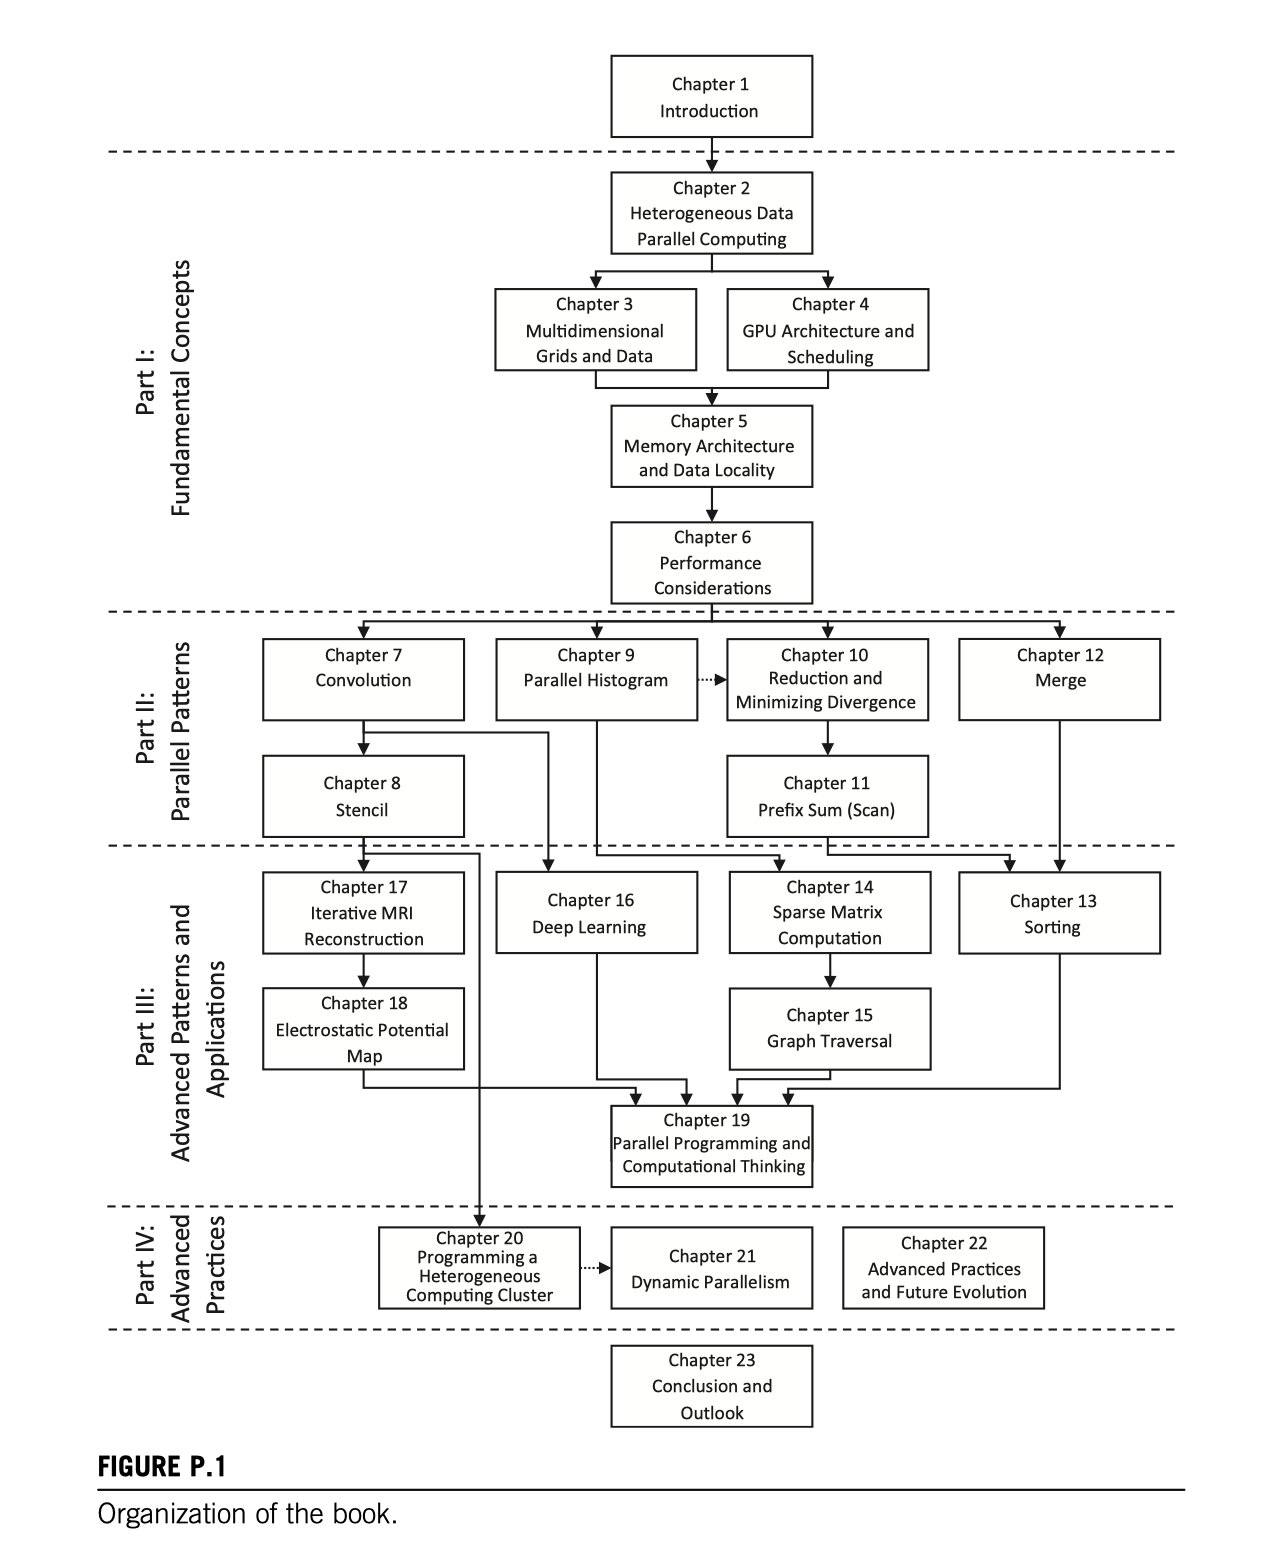
\includegraphics[width=\textwidth]{figs/P.1.png}
\end{figure}

\subsection{如何使用这本书}
我们希望通过本书提供一些教学课程的经验。 自 2006 年以来,我们教授多种类型的课程:一学期课程和一周强化课程。 
最初的 ECE498AL 课程已成为伊利诺伊大学香槟分校的永久课程,称为 ECE408 或 CS483。 
当我们第二次提供 ECE498AL 时,我们开始编写本书的一些早期章节。 
前四章也在 Nicolas Pinto 于 2009 年春天教授的麻省理工学院课程中进行了测试。
从那时起,我们将这本书用于 ECE408 的众多课程以及 Coursera 异构并行编程课程以及 VSCSE 和 PUMPS 暑期学校 。

\subsection{两阶段方法}
书中的大部分章节都设计为每节大约 75 分钟的讲座。 可能需要两节 75 分钟的讲座才能完全讲完的章节
是第 11 章(前缀和(扫描))、第 14 章(稀疏矩阵计算)和第 15 章(图遍历)。 
在 ECE408 中,讲座、编程作业和期末项目是同步进行的,并分为两个阶段。

在第一阶段,即本书的第一部分和第二部分,学生学习基础知识和基本模式,并练习通过指导性编程作业所学到的技能。 
此阶段由 12 章组成,通常需要大约 7 周的时间。 每周,学生都会完成与该周讲座相对应的编程作业。 
例如,第一周,基于第2章的讲座专门讲授基本的CUDA内存/线程模型、CUDA对C语言的扩展以及基本的编程工具。 
讲座结束后,学生可以在几个小时内编写简单的向量加法代码。

接下来的两周包括基于第 3 章到第 6 章的一系列四堂讲座,让学生对 CUDA 内存模型、CUDA 线程执行模型、
GPU 硬件性能特征和现代计算机系统架构有概念性的理解。 
在这两周内,学生们研究矩阵-矩阵乘法的不同实现,他们会看到在此期间其实现的性能如何显着提高。 
在剩下的四个星期中,讲座涵盖了基于第 7 章到第 12 章开发高性能并行应用程序所需的常见数据并行编程模式。
在这几周中,学生完成有关卷积、直方图、约简和前缀和的作业。 在第一阶段结束时,学生应该对并行编程非常熟悉,
并且应该准备好以更少的操作来实现更高级的代码。

在第二阶段(由第三部分和第四部分组成)中,学生在完成涉及加速高级模式或应用程序的最终项目时学习高级模式和应用程序。 
他们还学习了在完成项目时可能会发现有用的高级实践。 尽管我们通常不会在此阶段分配每周的编程作业,
但该项目通常有一个每周里程碑来帮助学生调整自己的节奏。 根据课程的持续时间和形式,教师可能无法涵盖此阶段的所有章节,
可能需要跳过一些章节。 教师还可以选择用客座讲座、论文讨论会或支持最终项目的讲座来代替一些讲座。 
因此,图 P.1 使用箭头来指示章节之间的依赖关系,以帮助教师选择可以跳过或重新排序的章节,以根据其特定上下文定制课程。

\subsection{将它们结合在一起:最终项目}
虽然本书的讲座、实验和章节有助于为学生奠定知识基础,但将学习经验整合在一起的是最终项目。 
最终项目对于整个学期的课程非常重要,因此它在课程中占据显着位置,需要近两个月的时间来重点关注。 
它包含五个创新方面:指导、研讨会、临床、最终报告和研讨会。 
虽然有关最终项目的大部分信息都可以在伊利诺伊州 NVIDIA GPU 教学套件中找到,但我们仍想提供这些方面设计背后的推理。

鼓励学生将他们的最终项目基于代表研究界当前挑战的问题。 为了推动这一过程,
教师应该招募几个计算科学研究小组来提出问题并担任导师。 导师被要求提供一份一到两页的项目规格表,
简要描述申请的重要性、导师希望与学生团队一起完成申请的目标、技术技能(特定类型的数学、物理) 和化学课程),
这是理解和使用应用程序所需的,以及学生可以利用的网络和传统资源列表,以获取技术背景、一般信息和构建块,
以及特定实现的特定 URL 或 FTP 路径 和编码示例。 
这些项目规格表还为学生提供了在其职业生涯后期定义自己的研究项目的学习经验。 
伊利诺伊州-NVIDIA GPU 教学套件中提供了几个示例。

\subsection{设计文档}
一旦学生决定了一个项目并组建了一个团队,他们就需要提交该项目的设计文件。 
这有助于他们在投入项目之前仔细考虑项目步骤。 进行此类规划的能力对于他们以后的职业成功非常重要。 
设计文件应讨论项目的背景和动机、应用程序级目标和潜在影响、最终应用程序的主要特征、
设计概述、实施计划、性能目标、验证计划和验收测试 ,以及项目进度表。

\subsection{项目报告及座谈会}
学生需要提交一份关于其团队主要发现的项目报告。 我们还建议举办全天的班级研讨会。 
在研讨会期间,学生使用与团队规模成比例的演示时段。 
在演示过程中,学生们为了全班同学的利益而突出了他们的项目报告中最好的部分。 
演讲占学生成绩的很大一部分。 每个学生必须单独回答针对该学生的问题,因此可以为同一团队中的个人分配不同的成绩。 
研讨会为学生提供了一个学习如何进行简洁演示的机会,以激励他们的同伴阅读全文。

\subsection{班级竞赛}
2016年ECE408的招生规模远远超过了最终项目进程所能容纳的水平。 结果,我们从期末项目变成了班级竞赛。 
在学期中期,我们宣布了一个竞赛挑战问题。 我们用一个讲座来解释比赛挑战问题以及用于对团队进行排名的规则。 
所有学生提交的内容都会自动评分和排名。 每个团队的最终排名取决于其并行代码的执行时间、正确性和清晰度。 
学生在学期结束时演示他们的解决方案并提交最终报告。 当班级规模导致最终项目不可行时,这种妥协保留了最终项目的一些好处。

\subsection{课程资源}
伊利诺伊州-NVIDIA GPU 教学套件是一个公开资源,其中包含讲座幻灯片和录音、实验作业、
最终项目指南以及为在课堂上使用本书的教师提供的示例项目规范。 此外,我们正在公开基于本书的伊利诺伊州本科生和研究生课程。 
虽然本书为这些课程提供了知识内容,但附加材料对于实现总体教育目标至关重要。

最后,我们鼓励您提交反馈。 如果您有任何改进本书的想法,我们希望收到您的来信。 我们想知道如何改进在线补充材料。 
当然,我们也想知道您喜欢这本书的哪些方面。 我们期待您的回音。


\newpage
\section*{致谢}
有很多人为第四版做出了特殊贡献。 我们首先要感谢各章节的合著者。 他们的名字列在他们做出特殊贡献的章节中。 
他们的专业知识对这个新版本的技术内容产生了巨大的影响。 如果没有这些人的专业知识和贡献,
我们就无法以我们希望向读者提供的洞察力来涵盖这些主题。

我们要特别感谢 CUDA 之父 Ian Buck 和 Tesla GPU 计算架构的首席架构师 John Nickolls。 
他们的团队为本课程构建了出色的基础设施。 NVIDIA 的许多工程师和研究人员也为 CUDA 的快速发展做出了贡献,
CUDA 支持高级并行模式的高效实现。 当我们制作第二版时,约翰去世了。 我们非常想念他。

自第三版以来,我们的外部审稿人花费了大量宝贵的时间为我们提供富有洞察力的反馈:
Sonia Lopez Alarcon(罗彻斯特理工学院)、Bedrich Benes(普渡大学)、Bryan Chin(加州大学圣地亚哥分校)、
Samuel Cho(维克森林大学) )、Kevin Farrell(爱尔兰都柏林布兰查兹敦理工学院)、
Lahouari Ghouti(沙特阿拉伯法赫德国王石油矿产大学)、Marisa Gil(西班牙巴塞罗那加泰罗尼亚理工大学)、
Karen L. Karavanic(波特兰) 州立大学)、Steve Lumetta(伊利诺伊大学厄巴纳-香槟分校)、
Dejan Milojici(惠普实验室)、Pinar Muyan-Ozcelik(加州州立大学萨克拉门托分校)、
Greg Peterson(田纳西大学诺克斯维尔分校)、Jose´L. Sa´nchez(卡斯蒂利亚拉曼恰大学)、
Janche Sang(克利夫兰州立大学)和 Jan Verschelde(伊利诺伊大学芝加哥分校)。 
他们的评论帮助我们显着提高了本书的内容和可读性。

Steve Merken、Kiruthika Govindaraju、Naomi Robertson 以及他们在爱思唯尔的员工为这个项目孜孜不倦地工作。

我们要特别感谢黄仁勋为开发这门课程提供了大量的财力和人力资源,为本书奠定了基础。

我们要感谢迪克·布拉胡特 (Dick Blahut),他向我们提出了启动该项目的挑战。 
Beth Katsinas 安排了 Dick Blahut 与 NVIDIA 副总裁 Dan Vivoli 的会面。 
通过那次聚会,Blahut 被介绍给 David,并挑战 David 来伊利诺伊州,与 Wen-mei. 一起创建原创的 ECE498AL 课程。

我们要特别感谢我们的同事 Kurt Akeley、Al Aho、Arvind、Dick Blahut、Randy Bryant、Bob Colwell、Bill Dally、
Ed Davidson、Mike Flynn、Michael Garland、John Hennessy、Pat Hanrahan、Nick Holonyak、Dick Karp、
Kurt Keutzer、Chris Lamb、Dave Liu、David Luebke、Dave Kuck、Nacho Navarro、Sanjay Patel、Yale Patt、
David Patterson、Bob Rao、Burton Smith、Jim Smith 和 Mateo Valero 花时间与我们分享了他们的见解 这些年来。

所有为这门课程和本书做出贡献的伟大人士的慷慨和热情让我们深感谦卑。


\newpage
\section{介绍}

自从计算出现以来,许多高价值应用程序都需要比计算设备所能提供的更高的执行速度和资源。 
早期应用依靠处理器速度、内存速度和内存容量的进步来增强应用级能力,如天气预报的及时性、工程结构分析的准确性、
计算机生成图形的真实性、航班预订数量等 每秒处理的资金转账数量。 
最近,深度学习等新应用程序需要比最好的计算设备所能提供的更多的执行速度和资源。 
这些应用需求在过去五年中推动了计算设备功能的快速进步,并且在可预见的未来将继续如此。

基于单个中央处理单元 (CPU) 的微处理器似乎按顺序步骤执行指令,例如 Intel 和 AMD 的 x86 处理器中的微处理器,
配备快速增加的时钟频率和硬件资源,推动了20世纪80年代和90年代的计算机应用性能的快速提高和成本的降低。 
在二十年的发展过程中,这些单 CPU 微处理器为桌面带来了 GFLOPS,即每秒千兆 ($10^9$) 次浮点运算,为数据中心带来了 TFLOPS,
即每秒万亿 ($10^{12}$) 次浮点运算。 这种对性能改进的不懈追求使得应用软件能够提供更多功能、
拥有更好的用户界面并生成更有用的结果。 反过来,一旦用户习惯了这些改进,他们就会要求更多的改进,
从而为计算机行业创造一个积极(良性)的循环。

然而,自 2003 年以来,由于能源消耗和散热问题,这种正向驱动的速度已经放缓。 
这些问题限制了时钟频率的增加以及单个 CPU 内每个时钟周期内可以执行的生产活动,同时保持了按顺序步骤执行指令的外观。 
从那时起,几乎所有微处理器供应商都转向了在每个芯片中使用多个物理 CPU(称为处理器内核)的模型,以提高处理能力。 
在这个模型中,传统的CPU可以被视为单核CPU。 为了受益于多个处理器内核,用户必须拥有多个指令序列,
无论是来自相同应用程序还是不同应用程序,都可以在这些处理器内核上同时执行。 对于要从多个处理器核心中受益的特定应用程序,
其工作必须分为可以在这些处理器核心上同时执行的多个指令序列。 
从单 CPU 按顺序执行指令到多核并行执行多个指令序列的转变对软件开发人员社区产生了巨大影响。

传统上,绝大多数软件应用程序都是作为顺序程序编写的,由处理器执行,
这些处理器的设计是冯·诺依曼在 1945 年的开创性报告中设想的(冯·诺依曼等人,1972 年)。 
人们可以将这些程序的执行理解为基于程序计数器(在文献中也称为指令指针)的概念按顺序单步执行代码。 
程序计数器包含处理器将执行的下一条指令的内存地址。 由应用程序的这种顺序、
逐步执行产生的指令执行活动序列在文献中被称为执行线程,或简称为线程。 线程的概念非常重要,
因此本书的其余部分将对其进行更正式的定义和广泛的使用。

从历史上看,大多数软件开发人员依赖硬件的进步,例如提高时钟速度和在后台执行多条指令,来提高顺序应用程序的速度; 
随着每一代新处理器的推出,相同的软件运行得更快。 计算机用户也越来越期望这些程序在每一代新一代微处理器上运行得更快。 
这种期望十多年来一直不成立。 顺序程序将仅在一个处理器内核上运行,一代又一代不会变得明显更快。 
如果没有性能改进,随着新微处理器的推出,应用程序开发人员将无法再在其软件中引入新的特性和功能; 
这减少了整个计算机行业的增长机会。

相反,每一代新一代微处理器将继续享受显着性能改进的应用软件将是并行程序,其中多个执行线程协作以更快地完成工作。 
并行程序相对于顺序程序的这种新的、显着提升的优势被称为并发革命(Sutter 和 Larus,2005)。 
并行编程的实践绝不是新鲜事。 几十年来,高性能计算 (HPC) 社区一直在开发并行程序。 
这些并行程序通常在昂贵的大型计算机上运行。 只有少数精英应用程序可以证明使用这些计算机是合理的,
从而将并行编程的实践限制在少数应用程序开发人员中。 现在所有新的微处理器都是并行计算机,
需要开发为并行程序的应用程序数量急剧增加。 现在软件开发人员非常需要学习并行编程,这也是本书的重点。

\subsection{异构并行计算}
自 2003 年以来,半导体行业已经确定了微处理器设计的两条主要轨迹(Hwu 等人,2008 年)。 
多核轨迹旨在在进入多核的同时保持顺序程序的执行速度。 多核始于两核处理器,并且核心数量随着每一代半导体工艺的发展而增加。 
最近的一个例子是最新的 Intel 多核服务器微处理器,具有多达 24 个处理器核心,每个处理器核心都是无序、多指令发布处理器,
实现完整的 x86 指令集,支持具有两个硬件线程的超线程,旨在最大限度地提高性能。 顺序程序的执行速度。 
另一个例子是最新的 ARM Ampere 多核服务器处理器,具有 128 个处理器内核。

相比之下,多线程轨迹更关注并行应用程序的执行吞吐量。 多线程轨迹始于大量线程,并且线程数量再次随着每一代的增加而增加。 
最近的一个例子是 NVIDIA Tesla A100 图形处理单元 (GPU),它具有数万个线程,在大量简单、有序的管道中执行。 
自 2003 年以来,多线程处理器,尤其是 GPU,一直在浮点性能竞赛中处于领先地位。
截至 2021 年,A100 GPU 的峰值浮点吞吐量为 64 位双精度 9.7 TFLOPS,32 位单精度 156 TFLOPS,
16 位半精度为 312 TFLOPS。 相比之下,最新的英特尔 24 核处理器的双精度峰值浮点吞吐量为 0.33 TLOPS,
单精度为 0.66 TFLOPS。 过去几年,多线程 GPU 和多核 CPU 之间的峰值浮点计算吞吐量之比一直在增加。 
这些不一定是应用程序速度; 它们只是这些芯片中执行资源可以支持的原始速度。

多核和多线程之间的峰值性能之间如此巨大的差距已经形成了显着的“电势”积累,在某些时候,必须做出一些让步。 
我们已经达到了这一点。 迄今为止,这种巨大的峰值性能差距已经促使许多应用程序开发人员将其软件的计算密集型部分转移到 
GPU 上执行。 也许更重要的是,并行执行性能的大幅提升使得革命性的新应用成为可能,例如本质上由计算密集型部分组成的深度学习。 
毫不奇怪,这些计算密集型部分也是并行编程的主要目标:当有更多工作要做时,
就有更多机会在协作的并行工作线程(即线程)之间分配工作。

{\color{red} Fig 1.1}

有人可能会问,为什么多线程 GPU 和多核 CPU 之间的峰值性能差距如此之大。 答案在于两种类型处理器之间基本设计理念的差异,
如图 1.1 所示。 如图 1.1A 所示,CPU 的设计针对顺序代码性能进行了优化。 
算术单元和操作数数据传送逻辑的设计旨在最大限度地减少算术运算的有效延迟,但代价是增加芯片面积和每单元功耗的使用。 
大型末级片上高速缓存旨在捕获频繁访问的数据,并将一些长延迟内存访问转换为短延迟高速缓存访问。 
复杂的分支预测逻辑和执行控制逻辑用于减轻条件分支指令的延迟。 通过减少操作的延迟,CPU 硬件减少了每个单独线程的执行延迟。 
然而,低延迟算术单元、复杂的操作数传送逻辑、大型高速缓冲存储器和控制逻辑消耗了芯片面积和功率,
否则这些芯片面积和功率可用于提供更多算术执行单元和存储器访问通道。 这种设计方法通常称为面向延迟的设计。

另一方面,GPU 的设计理念是由快速发展的视频游戏行业塑造的,
该行业对在高级游戏中执行大量浮点计算和每帧内存访问的能力提出了巨大的经济压力。 
这种需求促使 GPU 供应商寻找方法来最大化专用于浮点计算和内存访问吞吐量的芯片面积和功率预算。

在图形应用程序中,每秒执行大量浮点计算以完成视点变换和对象渲染等任务是非常直观的。 
此外,每秒执行大量内存访问的需求同样重要,甚至可能更重要。 
许多图形应用程序的速度受到数据从内存系统传送到处理器的速率的限制,反之亦然。 
GPU 必须能够将大量数据移入和移出其 DRAM(动态随机存取存储器)中的图形帧缓冲区,
因为这种移动可以使视频显示丰富并满足游戏玩家的需求。 
游戏应用程序普遍接受的宽松内存模型(各种系统软件、应用程序和 I/O 设备期望其内存访问工作的方式)
也使 GPU 更容易支持访问内存的大规模并行性。

相比之下,通用处理器必须满足传统操作系统、应用程序和 I/O 设备的要求,这些要求对支持并行内存访问提出了更多挑战,
从而使提高内存访问(通常称为内存)的吞吐量,常被称为内存带宽,变得更加困难。 
因此,图形芯片的运行内存带宽大约是同时可用 CPU 芯片的 10 倍,我们预计 GPU 在内存带宽方面将在一段时间内继续保持优势。

一个重要的观察是,就功耗和芯片面积而言,减少延迟比增加吞吐量要昂贵得多。 
例如,可以通过将运算单元的数量加倍来使运算吞吐量加倍,但代价是芯片面积和功耗加倍。 
然而,将算术延迟减少一半可能需要将电流加倍,但代价是所用芯片面积增加一倍以上,功耗增加四倍。 
因此,GPU 的主流解决方案是优化大量线程的执行吞吐量,而不是减少单个线程的延迟。 
这种设计方法允许流水线内存通道和算术运算具有较长的延迟,从而节省了芯片面积和功耗。 
内存访问硬件和算术单元的面积和功率的减少使得 GPU 设计者可以在芯片上拥有更多的硬件和算术单元,从而提高总执行吞吐量。 
图 1.1 通过在图 1.1A 的 CPU 设计中显示较少数量的较大算术单元和较少数量的内存通道,直观地说明了设计方法的差异,
与图 1.1B 中大量的较小算术单元和大量的存储器通道形成对比。

这些 GPU 的应用软件预计将使用大量并行线程编写。 当其中一些线程等待长延迟内存访问或算术运算时,
硬件会利用大量线程来寻找要做的工作。 图 1.1B 中的小型高速缓冲存储器用于帮助控制这些应用程序的带宽需求,
以便访问相同内存数据的多个线程不需要全部访问 DRAM。 这种设计风格通常称为面向吞吐量的设计,
因为它力求最大化大量线程的总执行吞吐量,同时允许单个线程可能需要更长的执行时间。

应该清楚的是,GPU 被设计为并行的、面向吞吐量的计算引擎,它们在某些 CPU 设计为能很好执行的任务上表现不佳。 
对于只有一个或很少线程的程序,具有较低操作延迟的CPU可以获得比GPU高得多的性能。 
当程序有大量线程时,具有较高执行吞吐量的GPU可以获得比CPU高得多的性能。 
因此,我们应该预料到许多应用程序会同时使用 CPU 和 GPU,在 CPU 上执行顺序部分,在 GPU 上执行数值密集型部分。 
这就是 NVIDIA 于 2007 年推出的统一计算设备架构 (CUDA) 编程模型旨在支持应用程序的 CPU-GPU 联合执行的原因。

还需要注意的是,当应用程序开发人员选择运行其应用程序的处理器时,速度并不是唯一的决定因素。 其他几个因素可能更为重要。 
首先也是最重要的是,所选处理器必须在市场上占有很大的份额,称为处理器的安装基础。 原因很简单。 
大量的客户群最能证明软件开发成本的合理性。 在市场份额较小的处理器上运行的应用程序不会有大量的客户群。 
这一直是传统并行计算系统的一个主要问题,与通用微处理器相比,传统并行计算系统的市场份额可以忽略不计。 
只有少数由政府和大公司资助的精英应用程序在这些传统的并行计算系统上成功开发。 多线程 GPU 改变了这种情况。 
由于 GPU 在 PC 市场的受欢迎,其销量已达数亿。 几乎所有台式电脑和高端笔记本电脑都配备了 GPU。 
迄今为止,已使用超过 10 亿个支持 CUDA 的 GPU。 如此庞大的市场占有率使这些 GPU 对应用程序开发人员来说具有经济吸引力。

另一个重要的决定因素是实用的外形因素和易于访问性。 直到 2006 年,并行软件应用程序都在数据中心服务器或部门集群上运行。 
但这样的执行环境往往会限制这些应用程序的使用。 比如在医学影像这样的应用中,发表一篇基于64节点集群机的论文就可以了。 
但磁共振成像 (MRI) 机器的实际临床应用是基于 PC 和特殊硬件加速器的某种组合。 
原因很简单,GE 和西门子等制造商无法在临床环境中销售需要计算机服务器机架的 MRI,而这在学术部门环境中很常见。 
事实上,美国国立卫生研究院 (NIH) 在一段时间内拒绝资助并行编程项目; 他们认为并行软件的影响将是有限的,
因为基于集群的大型机器无法在临床环境中工作。 如今,许多公司都配备了 GPU 的 MRI 产品,
美国国立卫生研究院 (NIH) 也资助使用 GPU 计算的研究。

直到 2006 年,图形芯片都非常难以使用,因为程序员必须使用相当于图形 API(应用程序编程接口)功能来访问处理单元,
这意味着需要 OpenGL 或 Direct3D 技术来对这些芯片进行编程。 更简单地说,计算必须表示为以某种方式绘制像素的函数,
以便在这些早期的 GPU 上执行。 该技术称为 GPGPU,用于使用 GPU 进行通用编程。 即使使用更高级别的编程环境,
底层代码仍然需要适合用于绘制像素的 API。 这些 API 限制了人们实际上可以为早期 GPU 编写的应用程序类型。 
因此,GPGPU 并没有成为一种广泛的编程现象。 尽管如此,这项技术还是足够令人兴奋,激发了一些英勇的努力和出色的研究成果。

2007 年,随着 CUDA 的发布,一切都发生了变化(NVIDIA,2007)。 CUDA 并不单独代表软件变更; 
芯片中添加了额外的硬件。 NVIDIA实际上专门投入了硅片面积以方便并行编程。 在 G80 及其后续并行计算芯片中,
GPGPU 程序根本不再通过图形接口。 相反,硅芯片上的新通用并行编程接口可以满足 CUDA 程序的要求。 
通用编程接口极大地扩展了可以轻松为 GPU 开发的应用程序类型。 所有其他软件层也都重新设计,
以便程序员可以使用熟悉的 C/C++ 编程工具。

虽然 GPU 是异构并行计算中的一类重要计算设备,但还有其他重要类型的计算设备在异构计算系统中用作加速器。 
例如,现场可编程门阵列已被广泛用于加速网络应用。 本书中介绍的使用 GPU 作为学习工具的技术也适用于这些加速器的编程任务。

\subsection{为什么要提高速度或并行性?}
正如我们在 1.1 节中所述,大规模并行编程的主要动机是让应用程序在未来的硬件世代中享受持续的速度提升。 
正如我们将在并行模式、高级模式和应用程序(第二部分和第三部分,第 7 章到第 19 章)中讨论的那样,
当应用程序适合并行执行时,在 GPU 上良好的实现可以比在单个 CPU 内核上顺序执行获得 100 倍以上的加速。
如果应用程序包含我们所说的“数据并行性”,通常只需几个小时的工作即可实现 10x 的加速。

人们可能会问为什么应用程序将继续要求提高速度。 我们今天拥有的许多应用程序似乎运行得足够快。 
尽管当今世界有无数的计算应用程序,但未来许多令人兴奋的大众市场应用程序都是我们之前认为的超级计算应用程序或超级应用程序。 
例如,生物学研究界正在越来越多地进入分子水平。 显微镜可以说是分子生物学中最重要的仪器,过去依赖光学或电子仪器。 
然而,我们使用这些仪器进行的分子水平观察存在局限性。 通过结合计算模型来模拟具有传统仪器设置的边界条件的基础分子活动,
可以有效地解决这些限制。 通过模拟,我们可以测量更多的细节并测试更多的假设,这比仅使用传统仪器所能想象的要多。 
在可预见的未来,就可建模的生物系统的规模以及可在可容忍响应时间内模拟的反应时间长度而言,这些模拟将继续受益于计算速度的提高。 
这些增强将对科学和医学产生巨大影响。

对于视频和音频编码和操作等应用,请考虑与旧式 NTSC 电视相比,我们对数字高清 (HD) 电视的满意度。 
一旦我们在高清电视上体验到图像的细节水平,就很难再回到旧技术了。 但请考虑高清电视所需的所有处理。 
这是一个高度并行的过程,三维 (3D) 成像和可视化也是如此。 
未来,视图合成和低分辨率视频的高分辨率显示等新功能将需要电视具有更高的计算能力。 
在消费者层面,我们将开始看到越来越多的视频和图像处理应用程序,这些应用程序可以改善图片和视频的焦点、光照和其他关键方面。

更高的计算速度带来的好处之一是更好的用户界面。 智能手机用户现在可以享受到与大屏幕电视相媲美的高分辨率触摸屏的更自然的界面。 
毫无疑问,这些设备的未来版本将整合具有 3D 视角的传感器和显示器、
结合虚拟和物理空间信息以增强可用性的应用程序以及基于语音和计算机视觉的界面,从而需要更高的计算速度。

消费电子游戏领域也正在进行类似的发展。 过去,在游戏中驾驶汽车只是一组预先安排好的场景。 
如果你的车撞到了障碍物,你的车的路线不会改变; 只是游戏比分发生了变化。 您的车轮没有弯曲或损坏,即使您失去了一个车轮,
驾驶也不再困难。 随着计算速度的提高,游戏可以基于动态模拟而不是预先安排的场景。 
我们可以期待在未来体验到更多这样的现实效果。 事故会损坏你的车轮,你的在线驾驶体验将会更加真实。 
精确建模物理现象的能力已经激发了数字孪生的概念,其中物理对象在模拟空间中具有精确的模型,
从而可以以更低的成本彻底进行压力测试和恶化预测。 众所周知,物理效应的真实建模和模拟需要非常大量的计算能力。

通过大幅提高计算吞吐量而实现的新应用程序的一个重要例子是基于人工神经网络的深度学习。 
虽然神经网络自 20 世纪 70 年代以来一直在积极研究,但它们在实际应用中一直无效,
因为训练这些网络需要太多的标记数据和太多的计算。 互联网的兴起提供了大量带标签的图片,GPU 的兴起带来了计算吞吐量的激增。 
因此,自 2012 年以来,基于神经网络的应用在计算机视觉和自然语言处理领域得到了快速采用。
这种采用彻底改变了计算机视觉和自然语言处理应用,并引发了自动驾驶汽车和家庭辅助设备的快速发展。

我们提到的所有新应用程序都涉及以不同方式和在不同级别模拟和/或表示物理并发世界,并处理大量数据。 
有了如此大量的数据,大部分计算可以在数据的不同部分上并行完成,尽管它们必须在某些时候进行协调。 
在大多数情况下,数据交付的有效管理会对并行应用程序的可实现速度产生重大影响。 
虽然这样做的技术通常为一些每天使用此类应用程序的专家所熟知,
但绝大多数应用程序开发人员可以从对这些技术的更直观的理解和实际工作知识中受益。

我们的目标是以直观的方式向应用程序开发人员展示数据管理技术,这些开发人员的正规教育可能不是计算机科学或计算机工程。 
我们还旨在提供许多实用的代码示例和实践练习,帮助读者获取工作知识,
这需要一个实用的编程模型来促进并行实现并支持数据交付的正确管理。 CUDA 提供了这样的编程模型,
并且已经过大型开发者社区的充分测试。

\subsection{加速实际的应用}
通过并行化应用程序,我们可以期望获得多少加速? 计算系统 A 相对于计算系统 B 的应用程序加速比的定义是,
在系统 B 中执行应用程序所用的时间与在系统 A 中执行相同应用程序所用的时间之比。
例如,如果应用程序在系统 A 中执行需要花费 10 秒,而在系统 B 中执行需要 200 秒,
则系统 A 相对于系统 B 的执行加速为 200/10=20,称为 20x(20 倍)加速。

并行计算系统相对于串行计算系统可实现的加速取决于可以并行化的应用程序部分。 
例如,如果可并行部分所花费的时间百分比为 30\%,则并行部分加速 100x 将使应用程序的总执行时间减少不超过 29.7\%。 
也就是说,整个应用程序的加速大约仅为 1/(1 - 0.297)=1.42x。 事实上,即使在并行部分进行无限量的加速,
也只能将执行时间减少 30\%,实现的加速不超过 1.433。 
通过并行执行可以实现的加速水平可能会受到应用程序的可并行部分的严重限制,这一事实被称为阿姆达尔定律(Amdahl,2013)。 
另一方面,如果 99\% 的执行时间都在并行部分,则并行部分加速 100x 会将应用程序执行时间减少到原始时间的 1.99\%。 
这使整个应用程序加速了 50x。 因此,对于大规模并行处理器来说,应用程序的绝大多数执行都在并行部分进行,
以有效加快其执行速度,这一点非常重要。

研究人员已在某些应用程序中实现了超过 100x 的加速。 然而,这通常只有在算法得到增强后进行大量优化和调整才能实现,
这样超过 99.9\% 的应用程序工作都在并行部分。

应用程序可实现的加速水平的另一个重要因素是从内存访问和写入数据的速度。 在实践中,
应用程序的直接并行化通常会导致内存 (DRAM) 带宽饱和,从而仅带来大约 10x 的加速。 诀窍在于找出如何解决内存带宽限制,
这涉及到进行多种转换之一,以利用专门的 GPU 片上内存来大幅减少对 DRAM 的访问次数。 
然而,必须进一步优化代码以克服片上内存容量有限等限制。 本书的一个重要目标是帮助读者充分理解这些优化并熟练使用它们。

请记住,单核 CPU 执行所实现的加速水平也可以反映 CPU 对应用程序的适用性。 在某些应用程序中,CPU 的性能非常好,
这使得使用 GPU 加速性能变得更加困难。 大多数应用程序都有一些可以由 CPU 更好地执行的部分。 
我们必须给CPU一个公平的执行机会,并确保编写的代码能够让GPU补充CPU的执行,
从而正确地利用CPU/GPU组合系统的异构并行计算能力。 
截至目前,结合了多核 CPU 和众核 GPU 的大众市场计算系统已经为笔记本电脑带来了万亿级计算,为集群带来了百亿亿级计算。

{\color{red} Fig 1.2}

图 1.2 说明了典型应用的主要部分。 实际应用程序的大部分代码往往是连续的。 这些连续的部分被图示为桃子的“核”区域; 
尝试将并行计算技术应用于这些部分就像咬桃核一样——感觉不太好! 这些部分很难并行化。 CPU 在这些部分往往做得非常好。 
好消息是,虽然这些部分可能占用大部分代码,但它们往往只占超级应用程序执行时间的一小部分。

然后是我们所说的“桃肉”部分。 这些部分很容易并行化,一些早期的图形应用程序也是如此。 
异构计算系统中的并行编程可以极大地提高这些应用程序的速度。 如图1.2所示,早期的GPGPU编程接口只覆盖了桃肉部分的一小部分,
这类似于最令人兴奋的应用程序的一小部分。 正如我们将看到的,CUDA 编程接口旨在涵盖令人兴奋的应用程序的更大部分。 
并行编程模型及其底层硬件仍在快速发展,以实现更大的应用程序部分的高效并行化。

\subsection{并行编程中的挑战}
是什么让并行编程变得困难? 有人曾经说过,如果不关心性能,并行编程是很容易的。 您实际上可以在一小时内编写一个并行程序。 
但是,如果您不关心性能,为什么还要编写并行程序呢?

本书解决了在并行编程中实现高性能的几个挑战。 首先,设计具有与顺序算法相同的算法(计算)复杂度的并行算法可能具有挑战性。 
许多并行算法执行与顺序算法相同的工作量。 然而,一些并行算法比顺序算法做更多的工作。 事实上,有时他们可能会做太多的工作,
以至于最终在大型输入数据集上运行速度变慢。 这尤其是一个问题,因为快速处理大型输入数据集是并行编程的重要动机。

例如,许多现实世界的问题最自然地用数学递归来描述。 并行化这些问题通常需要以非直观的方式思考问题,
并且可能需要在执行过程中进行冗余工作。 有一些重要的算法原语,例如前缀和,可以促进将问题的顺序递归公式转换为更并行的形式。 
我们将更正式地介绍工作效率的概念,并将说明设计并行算法所涉及的方法和权衡,
这些算法可以使用重要的并行模式(例如第 11 章“前缀”中的前缀和)实现与顺序算法相同水平的计算复杂性 总和(扫描)。

其次,许多应用程序的执行速度受到内存访问延迟和/或吞吐量的限制。 我们将这些应用程序称为内存限制应用程序; 
相比之下,计算密集型应用程序受到每字节数据执行的指令数量的限制。 
在内存受限的应用程序中实现高性能并行执行通常需要提高内存访问速度的方法。 
我们将在第 5 章“内存架构和数据局部性”和第 6 章“性能注意事项”中介绍内存访问的优化技术,
并将在有关并行模式和应用程序的几个章节中应用这些技术。

第三,并行程序的执行速度通常比顺序程序的情况对输入数据特征更敏感。 许多现实世界的应用程序需要处理具有广泛变化特征的输入,
例如不稳定或不可预测的数据大小以及不均匀的数据分布。 这些大小和分布的变化可能会导致分配给并行线程的工作量不均匀,
并可能显着降低并行执行的效率。 并行程序的性能有时会因这些特征而发生巨大变化。 
我们将在介绍并行模式和应用程序的章节中介绍用于规范数据分布和/或动态细化线程数量的技术,以应对这些挑战。

第四,某些应用程序可以并行化,同时几乎不需要跨不同线程进行协作。 这些应用程序通常被称为“令人尴尬的并行”。 
其他应用程序需要线程相互协作,这需要使用同步操作,例如屏障或原子操作。 这些同步操作给应用程序带来了开销,
因为线程经常会发现自己在等待其他线程而不是执行有用的工作。 我们将在本书中讨论减少同步开销的各种策略。

幸运的是,研究人员已经解决了大部分挑战。 跨应用程序域还存在一些常见模式,
使我们能够将在一个域中派生的解决方案应用于其他域中的挑战。 
这是我们将在重要的并行计算模式和应用程序的背景下提出解决这些挑战的关键技术的主要原因。

\subsection{相关并行编程接口}
在过去的几十年里,人们提出了许多并行编程语言和模型(Mattson 等,2004)。 
最广泛使用的是用于共享内存多处理器系统的 OpenMP(Open,2005)和用于可扩展集群计算的消息传递接口(MPI)(MPI,2009)。 
两者都已成为主要计算机供应商支持的标准化编程接口。

OpenMP 实现由编译器和运行时组成。 程序员向 OpenMP 编译器指定有关循环的指令(命令)和编译指示(提示)。 
通过这些指令和编译指示,OpenMP 编译器可以生成并行代码。 运行时系统通过管理并行线程和资源来支持并行代码的执行。 
OpenMP 最初是为 CPU 执行而设计的,现已扩展为支持 GPU 执行。 OpenMP 的主要优点是它提供编译器自动化和运行时支持,
以从程序员那里抽象出许多并行编程细节。 
这种自动化和抽象有助于使应用程序代码在不同供应商生产的系统以及同一供应商的不同代系统之间更加可移植。 
我们将此属性称为性能可移植性。 然而,在 OpenMP 中进行有效的编程仍然需要程序员了解所涉及的所有详细的并行编程概念。 
由于 CUDA 为程序员提供了对这些并行编程细节的明确控制,因此即使对于那些想要使用 OpenMP 作为主要编程接口的人来说,
它也是一种极好的学习工具。 此外,根据我们的经验,OpenMP 编译器仍在不断发展和改进。 
许多程序员可能需要使用 CUDA 风格的接口来处理 OpenMP 编译器无法满足的部分。

另一方面,MPI 是一种编程接口,其中集群中的计算节点不共享内存(MPI,2009)。 
所有的数据共享和交互都必须通过显式的消息传递来完成。 MPI在HPC中得到了广泛的应用。 
用MPI编写的应用程序已在超过10万个节点的集群计算系统上成功运行。 如今,许多 HPC 集群都采用异构 CPU/GPU 节点。 
由于计算节点之间缺乏共享内存,将应用程序移植到 MPI 所需的工作量可能相当大。 
程序员需要执行域分解以跨各个节点划分输入和输出数据。 在域分解的基础上,
程序员还需要调用消息发送和接收函数来管理节点之间的数据交换。 相比之下,
CUDA 为 GPU 中的并行执行提供共享内存来解决这一难题。 虽然 CUDA 是与每个节点的有效接口,
但大多数应用程序开发人员需要使用 MPI 在集群级别进行编程。 
此外,通过 NVIDIA Collective Communications Library (NCCL) 等 API,CUDA 中的多 GPU 编程支持不断增加。 
因此,HPC 中的并行程序员了解如何在使用多 GPU 节点的现代计算集群中进行联合 MPI/CUDA 编程非常重要,
该主题将在第 20 章“异构计算集群编程”中介绍。

2009 年,包括 Apple、Intel、AMD/ATI 和 NVIDIA 在内的几家主要行业参与者联合开发了一种名为
开放计算语言 (OpenCL) 的标准化编程模型(The Khronos Group,2009)。 与 CUDA 类似,
OpenCL 编程模型定义了语言扩展和运行时 API,以允许程序员管理大规模并行处理器中的并行性和数据交付。 
与 CUDA 相比,OpenCL 更多地依赖 API,更少地依赖语言扩展。 
这使得供应商能够快速调整其现有的编译器和工具来处理 OpenCL 程序。 OpenCL 是一种标准化的编程模型,
用 OpenCL 开发的应用程序无需修改即可在所有支持 OpenCL 语言扩展和 API 的处理器上正确运行。 
然而,人们可能需要修改应用程序才能实现新处理器的高性能。

熟悉 OpenCL 和 CUDA 的人都知道,OpenCL 和 CUDA 的关键概念和功能之间存在显着的相似性。 
也就是说,CUDA程序员可以以最小的努力学习OpenCL编程。 更重要的是,
几乎所有在使用 CUDA 中学到的技术都可以轻松应用于 OpenCL 编程。

\subsection{总体目标}
我们的主要目标是教读者如何对大规模并行处理器进行编程以实现高性能。 
因此,本书的大部分内容都致力于开发高性能并行代码的技术。 我们的方法不需要大量的硬件专业知识。 
然而,您需要对并行硬件架构有一个很好的概念性理解,以便能够推断代码的性能行为。 
因此,我们将用一些篇幅来直观地理解基本的硬件架构特性,并用许多篇幅来介绍开发高性能并行程序的技术。 
特别是,我们将重点关注计算思维(Wing,2006)技术,这些技术将使您能够以适合大规模并行处理器上高性能执行的方式思考问题。

大多数处理器上的高性能并行编程需要了解硬件的工作原理。 可能需要很多年才能构建工具和机器,
使程序员能够在没有这些知识的情况下开发高性能代码。 即使我们有这样的工具,
我们怀疑了解硬件知识的程序员将能够比那些不了解硬件的程序员更有效地使用这些工具。 
因此,我们专门用第 4 章“计算架构和调度”来介绍 GPU 架构的基础知识。 
作为高性能并行编程技术讨论的一部分,我们还讨论了更专业的体系结构概念。

我们的第二个目标是教授并行编程的正确功能和可靠性,这是并行计算中的一个微妙问题。 
过去从事并行系统工作的程序员都知道,仅实现初始性能是不够的。 挑战在于以一种可以调试代码并支持用户的方式来实现它。 
CUDA 编程模型鼓励使用简单形式的屏障同步、内存一致性和原子性来管理并行性。 
此外,它还提供了一系列强大的工具,使人们不仅可以调试功能方面,还可以调试性能瓶颈。 
我们将证明,通过关注数据并行性,可以在应用程序中实现高性能和高可靠性。

我们的第三个目标是通过探索并行编程方法来实现未来硬件各代的可扩展性,
以便未来的机器(将越来越并行)可以比今天的机器更快地运行代码。 我们希望帮助您掌握并行编程,
以便您的程序可以扩展到新一代机器的性能水平。 这种可扩展性的关键是规范和本地化内存数据访问,
以最大限度地减少关键资源的消耗和更新数据结构时的冲突。 
因此,开发高性能并行代码的技术对于确保应用程序未来的可扩展性也很重要。

实现这些目标需要大量的技术知识,因此我们将在本书中介绍并行编程的相当多的原理和模式(Mattson et al., 2004)。 
我们不会单独教授这些原则和模式。 我们将在并行化有用应用程序的背景下教授他们。 
然而,我们无法涵盖所有这些技术,因此我们选择了最有用且经过充分验证的技术来详细介绍。 
事实上,当前版本有关并行模式的章节数量显着增加。 现在我们准备向您提供本书其余部分的快速概述。

\subsection{本书的组织}
本书分为四个部分。 第一部分涵盖并行编程、数据并行、GPU 和性能优化的基本概念。 
这些基础章节为读者提供了成为 GPU 程序员所需的基本知识和技能。 第二部分介绍了原始并行模式,
第三部分介绍了更高级的并行模式和应用程序。 这两部分应用了第一部分中学到的知识和技能,
并根据需要介绍了其他 GPU 架构特性和优化技术。 最后一部分(第四部分)介绍了高级实践,
以帮助想要成为专家 GPU 程序员的读者完善知识。

关于基本概念的第一部分由第 2 章至第 6 章组成。 第 2 章,异构数据并行计算,介绍数据并行性和 CUDA C 编程。 
本章依赖于读者之前具有 C 编程经验的事实。 它首先介绍了 CUDA C 作为 C 的简单、小型扩展,
支持异构 CPU/GPU 计算和广泛使用的单程序、多数据并行编程模型。 
然后,它涵盖了以下方面所涉及的思维过程:(1) 识别要并行化的应用程序部分,
(2) 隔离并行化代码要使用的数据,使用 API 函数在并行计算设备上分配内存, (3)使用API函数将数据传输到并行计算设备,
(4)将并行部分开发为将由并行线程执行的内核函数,(5)启动由并行线程执行的内核函数,
以及( 6) 最终通过 API 函数调用将数据传输回主机处理器。 我们使用向量加法的运行示例来说明这些概念。 
虽然本章的目标是教授 CUDA C 编程模型的足够概念,以便读者能够编写简单的并行 CUDA C 程序,
但它涵盖了开发基于任何并行编程接口的并行应用程序所需的几种基本技能。

第 3 章“多维网格和数据”介绍了 CUDA 并行执行模型的更多细节,特别是它涉及使用线程的多维组织处理多维数据。 
它对线程的创建、组织、资源绑定和数据绑定提供了足够的洞察力,使读者能够使用 CUDA C 实现复杂的计算。

第 4 章,计算架构和调度,介绍 GPU 架构,重点介绍如何组织计算核心以及如何调度线程在这些核心上执行。 
讨论了各种架构注意事项,以及它们对 GPU 架构上执行的代码性能的影响。 其中包括透明可扩展性、SIMD 执行和控制发散、
多线程和延迟容忍以及占用等概念,所有这些都在本章中进行了定义和讨论。

第 5 章“内存架构和数据局部性”通过讨论 GPU 的内存架构来扩展第 4 章“计算架构和调度”。 
它还讨论了可用于保存 CUDA 变量以管理数据传输和提高程序执行速度的特殊存储器。 
我们介绍分配和使用这些内存的 CUDA 语言功能。 适当地使用这些存储器可以极大地提高数据访问吞吐量,
并有助于缓解存储器系统中的流量拥塞。

第 6 章“性能注意事项”介绍了当前 CUDA 硬件中的几个重要的性能注意事项。 
特别是,它提供了有关所需的线程执行和内存访问模式的更多详细信息。 
这些细节构成了程序员推理其组织计算和数据决策的后果的概念基础。 
本章最后列出了 GPU 程序员经常用来优化任何计算模式的常见优化策略清单。 
该清单将在本书的接下来的两部分中使用,以优化各种并行模式和应用程序。

关于原始并行模式的第二部分由第 7 章至第 12 章组成。 第 7 章“卷积”介绍了卷积,这是一种常用的并行计算模式,
植根于数字信号处理和计算机视觉,需要仔细管理数据访问局部性。 我们还使用这种模式在现代 GPU 中引入恒定内存和缓存。 
第 8 章“模板”介绍了模板,这是一种类似于卷积的模式,但植根于求解微分方程,
并且具有为进一步优化数据访问局部性提供独特机会的特定功能。 我们还使用此模式来介绍线程和数据的 3D 组织,
并展示第 6 章“性能注意事项”中介绍的针对线程粒度的优化。

第 9 章“并行直方图”介绍了直方图,这是一种广泛用于统计数据分析以及大型数据集中的模式识别的模式。 
我们还使用这种模式引入原子操作作为协调共享数据并发更新和私有化优化的手段,从而减少了这些操作的开销。 
第 10 章“归约和最小化分支”介绍了归约树模式,该模式用于总结输入数据的集合。 
我们还使用此模式来演示控制分支发散对性能的影响,并展示如何减轻这种影响的技术。 
第 11 章“前缀和(扫描)”介绍了前缀和或扫描,这是一种重要的并行计算模式,它将固有的顺序计算转换为并行计算。 
我们还使用这种模式来引入并行算法中工作效率的概念。 最后,第 12 章“合并”介绍了并行合并,
这是一种在分而治之工作分区策略中广泛使用的模式。 我们还用本章来介绍动态输入数据的识别和组织。

关于高级并行模式和应用程序的第三部分在精神上与第二部分类似,但所涵盖的模式更详细,并且通常包含更多应用程序上下文。 
因此,这些章节不太关注介绍新技术或功能,而是更关注特定于应用程序的注意事项。 对于每个应用程序,
我们首先确定制定并行执行基本结构的替代方法,然后推理每个替代方案的优点和缺点。 
然后,我们完成实现高性能所需的代码转换步骤。 这些章节帮助读者将前面章节中的所有材料放在一起,
并在他们承担自己的应用程序开发项目时为他们提供支持。

第三部分由第 13 章至第 19 章组成。 第 13 章“排序”介绍了并行排序的两种形式:基数排序和合并排序。 
这种高级模式利用了前面章节中介绍的更原始的模式,特别是前缀和和并行合并。 第 14 章,稀疏矩阵计算,介绍了稀疏矩阵计算,
它广泛用于处理非常大的数据集。 本章向读者介绍了重新排列数据以实现更有效的并行访问的概念:数据压缩、填充、排序、转置
和正则化。 第 15 章,图遍历,介绍图算法以及如何在 GPU 编程中有效地实现图搜索。 提出了许多不同的并行图算法策略,
并讨论了图结构对最佳算法选择的影响。 这些策略建立在更原始的模式之上,例如直方图和合并。

第 16 章“深度学习”涵盖了深度学习,它正在成为 GPU 计算的一个极其重要的领域。 我们介绍了卷积神经网络的有效实现,
并将更深入的讨论留给其他来源。 卷积神经网络的高效实现利用了平铺等技术和卷积等模式。 第 17 章,迭代磁共振成像重建,
涵盖非笛卡尔 MRI 重建以及如何利用循环融合和分散-聚集变换等技术来增强并行性并减少同步开销。 第 18 章,静电势图,
涵盖了分子可视化和分析,这得益于通过应用稀疏矩阵计算中的经验教训来处理不规则数据的技术。

第 19 章“并行编程和计算思维”介绍了计算思维,即以更适合 HPC 的方式制定和解决计算问题的艺术。 
它通过涵盖组织程序的计算任务以使它们可以并行完成的概念来实现这一点。 我们首先讨论将抽象的科学、
特定问题的概念组织成计算任务的转化过程,这是生产高质量串行或并行应用软件的重要的第一步。 
然后本章讨论并行算法结构及其对应用程序性能的影响,这是基于 CUDA 性能调优经验。 
尽管我们没有深入探讨这些替代并行编程风格的实现细节,
但我们希望读者能够利用在本书中获得的基础来学习其中任何一种编程风格的编程。 
我们还提出了一个高级案例研究,以展示通过创造性计算思维可以看到的机会。

第四部分高级实践由第 20 至 22 章组成。 第 20 章,异构计算集群编程,介绍了异构集群上的 CUDA 编程,
其中每个计算节点都由 CPU 和 GPU 组成。 
我们讨论使用 MPI 和 CUDA 来集成节点间计算和节点内计算以及由此产生的通信问题和实践。 
第 21 章“CUDA 动态并行性”介绍了动态并行性,即 GPU 根据数据或程序结构动态为自身创建工作的能力,
而不是总是等待 CPU 这样做。 第 22 章“高级实践和未来发展”列出了 CUDA 程序员需要了解的重要的各种高级功能和实践。 
其中包括零复制内存、统一虚拟内存、多个内核同时执行、函数调用、异常处理、调试、分析、双精度支持、
可配置缓存/暂存器大小等主题。 例如,早期版本的 CUDA 在 CPU 和 GPU 之间提供有限的共享内存功能。 
程序员需要显式管理 CPU 和 GPU 之间的数据传输。 然而,当前版本的 CUDA 支持统一虚拟内存和零拷贝内存等功能,
可实现 CPU 和 GPU 之间的数据无缝共享。 有了这样的支持,CUDA 程序员可以将变量和数据结构声明为在 CPU 和 GPU 之间共享。 
运行时硬件和软件保持一致性,并根据需要自动代表程序员执行优化的数据传输操作。 
这种支持显着降低了与计算和 I/O 活动重叠的数据传输所涉及的编程复杂性。 在教科书的介绍部分,
我们使用 API 进行显式数据传输,以便读者更好地了解幕后发生的情况。 
我们稍后会在第 22 章“高级实践和未来演进”中介绍统一虚拟内存和零拷贝内存。

虽然本书中的章节都是基于 CUDA 的,但它们总体上帮助读者建立了并行编程的基础。 
我们相信,当我们从具体的例子中学习时,人类能够最好地理解。 也就是说,我们必须首先在特定编程模型的上下文中学习概念,
这为我们将知识推广到其他编程模型时提供了坚实的基础。 当我们这样做时,我们可以从 CUDA 示例中汲取具体经验。 
对CUDA的深入体验也使我们变得成熟,这将有助于我们学习甚至可能与CUDA模型无关的概念。

第 23 章“结论和展望”提供了结论性意见以及对大规模并行编程的未来的展望。 我们首先重新审视我们的目标,
并总结各章如何组合在一起以帮助实现目标。 最后,我们预测大规模并行计算的快速进步将使其成为未来十年最令人兴奋的领域之一。


\newpage
\section{异构数据并行计算}

数据并行是指对数据集的不同部分执行的计算工作可以彼此独立地完成,从而可以彼此并行地完成的现象。 许多应用程序表现出丰富的数据并行性,这使得它们适合可扩展的并行执行。 因此,并行程序员熟悉数据并行性的概念以及编写利用数据并行性的代码的并行编程语言结构非常重要。 在本章中,我们将使用 CUDA C 语言结构来开发一个简单的数据并行程序。

\subsection{数据并行}
当现代软件应用程序运行缓慢时,问题通常是数据——数据太多而无法处理。 图像处理应用程序处理具有数百万到数万亿像素的图像或视频。 科学应用程序使用数十亿个网格点对流体动力学进行建模。 分子动力学应用必须模拟数千到数十亿个原子之间的相互作用。 航空公司的调度涉及数千个航班、机组人员和机场登机口。 大多数像素、粒子、网格点、交互、飞行等通常可以在很大程度上独立处理。 例如,在图像处理中,将彩色像素转换为灰度仅需要该像素的数据。 模糊图像会平均每个像素的颜色与附近像素的颜色,仅需要该小像素邻域的数据。 即使是看似全局的操作,例如查找图像中所有像素的平均亮度,也可以分解为许多可以独立执行的较小计算。 这种对不同数据块的独立评估是数据并行性的基础。 编写数据并行代码需要(重新)组织围绕数据的计算,以便我们可以并行执行最终的独立计算,从而更快地完成整个工作——通常要快得多。

让我们通过一个彩色到灰度转换的例子来说明数据并行的概念。 图 2.1 显示了由许多像素组成的彩色图像(左侧),每个像素包含从 0(黑色)到 1(全强度)变化的红色、绿色和蓝色分数值(r、g、b)。

为了将彩色图像(图 2.1 左侧)转换为灰度图像(右侧),我们通过应用以下加权和公式计算每个像素的亮度值 L:
\begin{equation*}
	L = r*0.21 + g*0.72 + b * 0.07
\end{equation*}

\begin{remark}[RGB 彩色图像表示]
	在 RGB 表示中,图像中的每个像素都存储为 (r, g, b) 值的元组。 图像行的格式为 (r g b) (r g b) 。 。 。 (r g b),如下面的概念图所示。 每个元组指定红色 (R)、绿色 (G) 和蓝色 (B) 的混合。 也就是说,对于每个像素,r、g、b 值代表渲染该像素时红、绿、蓝光源的强度(0 为暗,1 为全强度)。

这三种颜色的实际允许混合因行业指定的颜色空间而异。 这里,AdbobeRGBt 颜色空间中三种颜色的有效组合显示为三角形的内部。 每个混合的垂直坐标(y 值)和水平坐标(x 值)显示应为 G 和 R 的像素强度分数。像素强度的剩余分数 (1-yÀx) 应分配给 B。 渲染图像时,每个像素的 r、g、b 值用于计算像素的总强度(亮度)以及混合系数(x、y、1-y-x)。
\end{remark}

如果我们将输入视为由 RGB 值数组 I 组织的图像,并将输出视为相应的亮度值数组 O,则我们得到如图 2.2 所示的简单计算结构。 例如,根据上式计算I[0]中RGB值的加权和,生成O[0]; O[1]是通过计算I[1]中RGB值的加权和生成的; O[2]是通过计算I[2]中RGB值的加权和生成的; 等等。 这些每像素计算都不相互依赖。 所有这些都可以独立执行。 显然,彩色到灰度的转换表现出丰富的数据并行性。 当然,完整应用程序中的数据并行性可能更加复杂,本书的大部分内容都致力于教授发现和利用数据并行性所必需的并行思维。

\begin{remark}[任务并行与数据并行]
数据并行并不是并行编程中使用的唯一并行类型。 任务并行性也广泛应用于并行编程中。 任务并行性通常通过应用程序的任务分解来暴露。 例如,一个简单的应用程序可能需要进行向量加法和矩阵向量乘法。 其中每一个都是一项任务。 如果两个任务可以独立完成,则存在任务并行性。 I/O 和数据传输也是常见的任务源。

在大型应用程序中,通常存在大量独立任务,因此任务并行性也较大。 例如,在分子动力学模拟器中,自然任务列表包括振动力、旋转力、非键合力的邻居识别、非键合力、速度和位置以及基于速度和位置的其他物理属性。

一般来说,数据并行性是并行程序可扩展性的主要来源。 对于大型数据集,人们通常可以找到丰富的数据并行性,以便能够利用大规模并行处理器,并允许应用程序性能随着每一代具有更多执行资源的硬件而增长。 尽管如此,任务并行性也可以在实现性能目标方面发挥重要作用。 稍后在介绍流时我们将介绍任务并行性。
\end{remark}

\subsection{CUDA C程序结构}
我们现在准备学习如何编写 CUDA C 程序来利用数据并行性来加快执行速度。 CUDA C 1 以最少的新语法和库函数扩展了流行的 ANSI C 编程语言,使程序员能够针对包含 CPU 内核和大规模并行 GPU 的异构计算系统。 顾名思义,CUDA C 构建在 NVIDIA 的 CUDA 平台上。 CUDA是目前最成熟的大规模并行计算框架。 它广泛应用于高性能计算行业,在最常见的操作系统上提供编译器、调试器和分析器等基本工具。

CUDA C 程序的结构反映了计算机中主机(CPU)和一个或多个设备(GPU)的共存。 每个 CUDA C 源文件可以混合有主机代码和设备代码。 默认情况下,任何传统 C 程序都是仅包含主机代码的 CUDA 程序。 人们可以将设备代码添加到任何源文件中。 设备代码清楚地标有特殊的 CUDA C 关键字。 设备代码包括函数或内核,其代码以数据并行方式执行。

CUDA 程序的执行如图 2.3 所示。 执行从主机代码(CPU 串行代码)开始。 当调用内核函数时,设备上会启动大量线程来执行内核。 由内核调用启动的所有线程统称为网格。 这些线程是 CUDA 平台中并行执行的主要工具。 图 2.3 显示了两个线程网格的执行情况。 我们将很快讨论这些网格是如何组织的。 当网格的所有线程都完成其执行时,网格终止,并且执行在主机上继续,直到启动另一个网格。 请注意,图 2.3 显示了一个简化模型,其中 CPU 执行和 GPU 执行不重叠。 许多异构计算应用程序管理重叠的 CPU 和 GPU 执行,以充分利用 CPU 和 GPU。

启动网格通常会生成许多线程来利用数据并行性。 在彩色到灰度转换的示例中,每个线程可用于计算输出数组 O 的一个像素。在这种情况下,网格启动应生成的线程数等于 图片。 对于大图像,会产生大量线程。 由于高效的硬件支持,CUDA 程序员可以假设这些线程只需很少的时钟周期即可生成和调度。 这一假设与传统的 CPU 线程形成对比,传统的 CPU 线程通常需要数千个时钟周期来生成和调度。 在下一章中,我们将展示如何实现颜色到灰度转换和图像模糊内核。 在本章的其余部分中,为了简单起见,我们将使用向量加法作为运行示例。

\begin{remark}[线程]
线程是现代计算机中处理器如何执行顺序程序的简化视图。 线程由程序代码、正在执行的代码中的点及其变量和数据结构的值组成。 就用户而言,线程的执行是顺序的。 人们可以使用源代码级调试器来监视线程的进度,方法是一次执行一个语句,查看下一个将要执行的语句,并在执行过程中检查变量和数据结构的值。

线程在编程中的应用已经很多年了。 如果程序员想要在应用程序中开始并行执行,他/她可以使用线程库或特殊语言创建和管理多个线程。 在 CUDA 中,每个线程的执行也是顺序的。 CUDA 程序通过调用内核函数来启动并行执行,这会导致底层运行时机制启动并行处理数据不同部分的线程网格。
\end{remark}

\subsection{向量加法核函数}
我们使用向量加法来演示 CUDA C 程序结构。 向量加法可以说是最简单的数据并行计算——相当于顺序编程中的“Hello World”。 在我们展示向量加法的内核代码之前,首先回顾一下传统向量加法(主机代码)函数的工作原理会很有帮助。 图 2.4 显示了一个简单的传统 C 程序,由主函数和向量加法函数组成。 在我们所有的示例中,每当需要区分主机和设备数据时,我们都会在主机使用的变量名称后添加“\_h”,在设备使用的变量名称后添加“\_d”以 提醒我们自己这些变量的预期用途。 由于图 2.4 中只有主机代码,因此我们只能看到后缀为“\_h”的变量。

假设要相加的向量存储在主程序中分配并初始化的数组A和B中。 输出向量位于数组C中,该数组也在主程序中分配。 为了简洁起见,我们没有显示 A、B 和 C 在主函数中如何分配或初始化的细节。 指向这些数组的指针连同包含向量长度的变量 N 一起传递给 vecAdd 函数。 请注意,vecAdd 函数的参数带有“\_h”后缀,以强调它们是由主机使用的。 当我们在接下来的几个步骤中引入设备代码时,这种命名约定将会很有帮助。

图 2.4 中的 vecAdd 函数使用 for 循环来迭代向量元素。 在第 i 次迭代中,输出元素 C\_h[i] 接收 A\_h[i] 和 B\_h[i] 的和。 向量长度参数 n 用于控制循环,使迭代次数与向量的长度相匹配。 该函数分别通过指针A\_h、B\_h和C\_h读取A和B的元素并写入C的元素。 当vecAdd函数返回时,main函数中的后续语句就可以访问C的新内容。

并行执行向量加法的一种直接方法是修改 vecAdd 函数并将其计算移至设备。 这种修改后的 vecAdd 函数的结构如图 2.5 所示。 该函数的第 1 部分在设备 (GPU) 内存中分配空间来保存 A、B 和 C 向量的副本,并将 A 和 B 向量从主机内存复制到设备内存。 第 2 部分调用实际的向量加法内核来启动设备上的线程网格。 第 3 部分将和向量 C 从设备内存复制到主机内存,并从设备内存中释放三个数组。

请注意,修改后的 vecAdd 函数本质上是一个外包代理,它将输入数据发送到设备,激活设备上的计算,并从设备收集结果。 代理这样做的方式是主程序甚至不需要知道矢量加法现在实际上是在设备上完成的。 在实践中,这种“透明”的外包模式可能非常低效,因为所有数据都来回复制。 人们通常会在设备上保留大型且重要的数据结构,并简单地从主机代码中调用它们上的设备功能。 不过,现在我们将使用简化的透明模型来介绍基本的 CUDA C 程序结构。 修改后的函数的细节以及内核函数的编写方式将是本章剩余部分的主题。

\subsection{设备全局内存和数据传输}
在当前的 CUDA 系统中,设备通常是硬件卡,带有自己的动态随机存取存储器,称为设备全局存储器,或简称为全局存储器。 例如,NVIDIA Volta V100 配备 16GB 或 32GB 全局内存。 将其称为“全局”内存,将其与程序员也可以访问的其他类型的设备内存区分开来。 有关 CUDA 内存模型和不同类型设备内存的详细信息将在第 5 章“内存架构和数据局部性”中讨论。

对于向量加法内核,在调用内核之前,程序员需要在设备全局内存中分配空间,并将数据从主机内存传输到设备全局内存中分配的空间。 这对应于图 2.5 的第 1 部分。 类似地,在设备执行之后,程序员需要将结果数据从设备全局存储器传输回主机存储器,并释放设备全局存储器中不再需要的已分配空间。 这对应于图 2.5 的第 3 部分。 CUDA运行时系统(通常在主机上运行)提供应用程序编程接口(API)函数来代表程序员执行这些活动。 从现在开始,我们将简单地说数据从主机传输到设备,作为数据从主机内存复制到设备全局内存的简写。 对于相反的方向也是如此。

图2.5中,vecAdd函数的第1部分和第3部分需要使用CUDA API函数为A、B和C分配设备全局内存; 将 A 和 B 从主机传输到设备; 向量相加后将 C 从设备传输到主机; 并释放A、B、C的设备全局内存。我们首先解释内存分配和释放函数。

图 2.6 显示了两个用于分配和释放设备全局内存的 API 函数。 可以从主机代码调用 cudaMalloc 函数来为对象分配一块设备全局内存。 读者应该注意到 cudaMalloc 和标准 C 运行时库 malloc 函数之间惊人的相似性。 这是故意的; CUDA C 是具有最少扩展的 C。 CUDA C使用标准C运行时库malloc函数来管理主机内存2,并将cudaMalloc作为C运行时库的扩展添加。 通过使接口尽可能接近原始 C 运行时库,CUDA C 最大限度地减少了 C 程序员重新学习这些扩展的使用所花费的时间。

cudaMalloc 函数的第一个参数是指针变量的地址,该变量将被设置为指向分配的对象。 指针变量的地址应转换为 (void à ),因为该函数需要一个通用指针; 内存分配函数是一个通用函数,不限于任何特定类型的对象。 3 该参数允许 cudaMalloc 函数将分配的内存的地址写入提供的指针变量,无论其类型如何。 4 调用内核的主机代码将此指针值传递给需要访问已分配内存对象的内核。 cudaMalloc 函数的第二个参数给出要分配的数据的大小(以字节数为单位)。 第二个参数的用法与 C malloc 函数的大小参数一致。

我们现在用下面简单的代码示例来说明cudaMalloc和cudaFree的使用:
\\
\\
\\
这是图 2.5 中示例的延续。 为了清楚起见,我们在指针变量后面加上“\_d”后缀,以指示它指向设备全局内存中的对象。 传递给 cudaMalloc 的第一个参数是转换为 void 指针的指针 A\_d(即 \&A\_d)的地址。 当cudaMalloc返回时,A\_d将指向为A向量分配的设备全局内存区域。 传递给 cudaMalloc 的第二个参数是要分配的区域的大小。 由于 size 是以字节数为单位的,因此程序员在确定 size 的值时需要将数组中的元素数转换为字节数。 例如,在为包含 n 个单精度浮点元素的数组分配空间时,size 的值将是单精度浮点数大小的 n 倍,在当今的计算机中为 4 个字节。 因此,size 的值将为 n × 4。计算后,以指针 A\_d 作为参数调用 cudaFree,以从设备全局内存中释放 A 向量的存储空间。 注意cudaFree不需要改变A\_d的值; 它只需要使用A\_d的值将分配的内存返回到可用池。 因此,只有 A\_d 的值而不是地址作为参数传递。

A\_d、B\_d 和 C\_d 中的地址指向设备全局内存中的位置。 这些地址不应在主机代码中取消引用。 它们应该用于调用API函数和内核函数。 在主机代码中取消引用设备全局内存指针可能会导致异常或其他类型的运行时错误。

读者应该使用类似的 B\_d 和 C\_d 指针变量声明及其相应的 cudaMalloc 调用来完成图 2.5 中 vecAdd 示例的第 1 部分。 此外,图 2.5 中的第 3 部分可以通过调用 B\_d 和 C\_d 的 cudaFree 来完成。

一旦主机代码在设备全局存储器中为数据对象分配了空间,它就可以请求将数据从主机传输到设备。 这是通过调用 CUDA API 函数之一来完成的。 图 2.7 显示了这样一个 API 函数 cudaMemcpy。 cudaMemcpy 函数有四个参数。 第一个参数是指向要复制的数据对象的目标位置的指针。 第二个参数指向源位置。 第三个参数指定要复制的字节数。 第四个参数表示复制涉及的内存类型:从主机到主机、从主机到设备、从设备到主机、从设备到设备。 例如,存储器复制功能可用于将数据从设备全局存储器中的一个位置复制到设备全局存储器中的另一位置。

vecAdd 函数调用 cudaMemcpy 函数,在相加之前将 A\_h 和 B\_h 向量从主机内存复制到设备内存中的 A\_d 和 B\_d,并在相加完成后将 C\_d 向量从设备内存复制到主机内存中的 C\_h 完毕。 假设 A\_h、B\_h、A\_d、B\_d 和 size 的值已经按照我们之前讨论的那样设置,则三个 cudaMemcpy 调用如下所示。 两个符号常量 cudaMemcpyHostToDevice 和 cudaMemcpyDeviceToHost 是 CUDA 编程环境可识别的预定义常量。 请注意,通过正确排序源指针和目标指针并使用适合传输类型的常量,可以使用同一函数在两个方向上传输数据。
\\
\\
\\

总而言之,图2.4中的主程序调用vecAdd,它也在主机上执行。 vecAdd 函数如图 2.5 所示,在设备全局内存中分配空间,请求数据传输,并调用执行实际向量加法的内核。 我们将这种类型的主机代码称为调用内核的存根。 我们在图 2.8 中展示了 vecAdd 函数的更完整版本。

与图2.5相比,图2.8中的vecAdd函数对于第1部分和第3部分来说是完整的。第1部分为A\_d、B\_d和C\_d分配设备全局内存,并将A\_h传输到A\_d,将B\_h传输到B\_d。 这是通过调用 cudaMalloc 和 cudaMemcpy 来完成的功能。 鼓励读者使用适当的参数值编写自己的函数调用,并将他们的代码与图 2.8 所示的代码进行比较。 第 2 部分调用内核,并将在下面的小节中描述。 第 3 部分将向量和数据从设备复制到主机,以便这些值在主函数中可用。 这是通过调用 cudaMemcpy 函数来完成的。 然后,它从设备全局内存中释放 A\_d、B\_d 和 C\_d 的内存,这是通过调用 cudaFree 函数来完成的(图 2.9)。

\subsection{核函数与线程}
我们现在准备更多地讨论 CUDA C 内核函数以及调用这些内核函数的效果。 在 CUDA C 中,内核函数指定在并行阶段由所有线程执行的代码。 由于所有这些线程都执行相同的代码,因此 CUDA C 编程是著名的单程序多数据 (SPMD)(Atallah,1998)并行编程风格的一个实例,这是并行计算系统的一种流行编程风格。 5

当程序的主机代码调用内核时,CUDA 运行时系统会启动组织成两级层次结构的线程网格。 每个网格都组织为线程块数组,为简洁起见,我们将其称为块。 网格中的所有块的大小相同; 在当前系统上,每个块最多可以包含 1024 个线程。 6 图 2.9 显示了一个示例,其中每个块由 256 个线程组成。 每个线程都由一个来自方框的卷曲箭头表示,该方框标有块中线程的索引号。

每个线程块中的线程总数由调用内核时的主机代码指定。 可以在主机代码的不同部分使用不同数量的线程来调用相同的内核。 对于给定的线程网格,块中的线程数可在名为 blockDim 的内置变量中获得。 blockDim 变量是一个具有三个无符号整数字段(x、y 和 z)的结构,可帮助程序员将线程组织成一维、二维或三维数组。 对于一维组织,仅使用 x 字段。 对于二维组织,使用 x 和 y 字段。 对于三维结构,使用所有三个 x、y 和 z 字段。 组织线程的维度选择通常反映了数据的维度。 这是有道理的,因为创建线程是为了并行处理数据,因此线程的组织很自然地反映了数据的组织。 在图2.9中,每个线程块被组织为一维线程数组,因为数据是一维向量。 blockDim.x变量的值表示每个块中的线程总数,在图2.9中为256。 一般来说,出于硬件效率的考虑,建议线程块每个维度的线程数量为32的倍数。 我们稍后会再讨论这个问题。

CUDA 内核可以访问另外两个内置变量(threadIdx 和 blockIdx),这些变量允许线程彼此区分并确定每个线程要处理的数据区域。 threadIdx 变量为每个线程提供块内的唯一坐标。 在图2.9中,由于我们使用一维线程组织,因此仅使用threadIdx.x。 每个线程的 threadIdx.x 值显示在图 2.9 中每个线程的小阴影框中。 每个块中的第一个线程的 threadIdx.x 变量的值为 0,第二个线程的值为 1,第三个线程的值为 2,依此类推。

blockIdx 变量为块中的所有线程提供一个公共块坐标。 在图 2.9 中,第一个块中的所有线程的 blockIdx.x 变量的值为 0,第二个线程块中的所有线程的值为 1,依此类推。 与电话系统进行类比,我们可以将 threadIdx.x 视为本地电话号码,将 blockIdx.x 视为区号。 两者共同为全国的每条电话线提供了唯一的电话号码。 类似地,每个线程可以组合其 threadIdx 和 blockIdx 值,在整个网格中为自己创建唯一的全局索引。

在图 2.9 中,唯一的全局索引 i 的计算公式为 i=blockIdx.x × blockDim。 x + 线程Idx.x。 回想一下,在我们的示例中,blockDim 是 256。 块 0 中线程的 i 值范围是 0 到 255。 块 1 中线程的 i 值范围是 256 到 511。 块 2 中线程的 i 值范围是 512 到 767。 这三个块中的线程形成了从 0 到 767 的值的连续覆盖。由于每个线程使用 i 访问 A、B 和 C,因此这些线程覆盖了原始循环的前 768 次迭代。 通过启动具有更多块的网格,可以处理更大的向量。 通过启动具有 n 个或更多线程的网格,可以处理长度为 n 的向量。

图 2.10 显示了向量加法的核函数。 请注意,我们不在内核中使用“\_h”和“\_d”约定,因为不存在潜在的混淆。 在我们的示例中,我们将无法访问主机内存。 内核的语法是 ANSI C,并带有一些值得注意的扩展。 首先,在 vecAddKernel 函数的声明前面有一个 CUDA-C 特定关键字“\_\_global\_\_”。 该关键字指示该函数是一个内核,并且可以调用它来在设备上生成线程网格。

一般来说,CUDA C 使用三个可在函数声明中使用的限定符关键字扩展了 C 语言。 这些关键字的含义总结在图 2.11 中。 “\_\_global\_\_”关键字表示所声明的函数是 CUDA C 内核函数。 请注意,“global”一词的两侧各有两个下划线字符。 这样的内核函数在设备上执行并且可以从主机调用。 在支持动态并行的 CUDA 系统中,也可以从设备调用它,我们将在第 21 章“CUDA 动态并行”中看到。 重要的特征是调用这样的内核函数会导致在设备上启动新的线程网格。

“\_\_device\_\_”关键字表示所声明的函数是 CUDA 设备函数。 设备函数在 CUDA 设备上执行,并且只能从内核函数或其他设备函数调用。 设备函数由调用它的设备线程执行,不会导致启动任何新的设备线程。7

“\_\_host\_\_”关键字表示所声明的函数是 CUDA 主机函数。 主机函数只是在主机上执行的传统 C 函数,并且只能从另一个主机函数调用。 默认情况下,如果 CUDA 程序中的所有函数在其声明中没有任何 CUDA 关键字,则它们都是主机函数。 这是有道理的,因为许多 CUDA 应用程序都是从纯 CPU 执行环境移植的。 程序员在移植过程中会添加内核函数和设备函数。 原始功能仍作为主机功能。 将所有函数默认为主机函数可以使程序员免去更改所有原始函数声明的繁琐工作。

请注意,可以在函数声明中同时使用“\_\_host\_\_”和“\_\_device\_\_”。 这种组合告诉编译系统为同一函数生成两个版本的目标代码。 一种是在主机上执行的,并且只能从主机函数中调用。 另一个在设备上执行,只能从设备或内核函数中调用。 当可以重新编译相同的函数源代码以生成设备版本时,这支持常见的用例。 许多用户库函数可能属于这一类。

C 的第二个值得注意的扩展,如图 2.10 所示,是内置变量“threadIdx”、“blockIdx”和“blockDim”。 回想一下,所有线程都执行相同的内核代码,并且需要有一种方法让它们彼此区分并将每个线程引导至数据的特定部分。 这些内置变量是线程访问为线程提供识别坐标的硬件寄存器的方法。 不同的线程将在其 threadIdx.x、blockIdx.x 和 blockDim.x 变量中看到不同的值。 为了便于阅读,我们有时会在讨论中将线程称为线程 blockIdx.x 、 threadIdx.x 。

图 2.10 中有一个自动(局部)变量 i。 在 CUDA 内核函数中,自动变量是每个线程私有的。 也就是说,将为每个线程生成一个 i 版本。 如果网格以 10,000 个线程启动,则 i 将会有 10,000 个版本,每个线程一个。 线程为其 i 变量分配的值对其他线程不可见。 我们将在第 5 章“内存架构和数据局部性”中更详细地讨论这些自动变量。

快速比较图 2.4 和图 2.10 揭示了对 CUDA 内核的重要见解。 图 2.10 中的核函数没有与图 2.4 中的循环相对应的循环。 读者应该问循环去了哪里。 答案是循环现在被线程网格所取代。 整个网格相当于循环。 网格中的每个线程对应于原始循环的一次迭代。 这有时称为循环并行,其中原始顺序代码的迭代由线程并行执行。

注意图 2.10 中的 addVecKernel 中有一个 if (i , n) 语句。 这是因为并非所有向量长度都可以表示为块大小的倍数。 例如,假设向量长度为 100。最小有效线程块维度为 32。假设我们选择 32 作为块大小。 需要启动 4 个线程块来处理所有 100 个向量元素。 然而,四个线程块将有 128 个线程。 我们需要禁止线程块 3 中的最后 28 个线程执行原始程序未预期的工作。 由于所有线程都将执行相同的代码,因此所有线程都将根据 n(即 100)测试其 i 值。使用 if (i , n) 语句,前 100 个线程将执行加法,而最后 28 个则不会。 这允许调用内核来处理任意长度的向量。

\subsection{调用核函数}
实现内核函数后,剩下的步骤是从主机代码调用该函数来启动网格。 如图 2.12 所示。 当主机代码调用内核时,它通过执行配置参数设置网格和线程块尺寸。 配置参数在传统 C 函数参数之前的“<<<”和“>>>”之间给出。 第一个配置参数给出了网格中的块数。 第二个指定每个块中的线程数。 在此示例中,每个块中有 256 个线程。 为了确保网格中有足够的线程来覆盖所有向量元素,我们需要将网格中的块数设置为所需线程数的上限除法(将商四舍五入到直接较高的整数值) (本例中为 n)乘以线程块大小(本例中为 256)。 有多种方法可以进行天花板划分。 一种方法是将 C 上限函数应用于 n/256.0。 使用浮点值 256.0 确保我们为除法生成一个浮点值,以便上限值函数可以正确地将其向上舍入。 例如,如果我们想要 1000 个线程,我们将启动 ceil(1000/256.0)5 4 个线程块。 结果,该语句将启动 4 3 2565 1024 个线程。 通过内核中的 if (i , n) 语句,如图 2.10 所示,前 1000 个线程将对 1000 个向量元素执行加法。 其余 24 个不会。

图 2.13 显示了 vecAdd 函数中的最终主机代码。 该源代码完成了图 2.5 中的框架。 无花果。 2.12和2.13共同说明了一个简单的CUDA程序,它由主机代码和设备内核组成。 该代码被硬连线为使用每个 256 个线程的线程块。 8 但是,所使用的线程块的数量取决于向量 (n) 的长度。 如果n为750,则将使用三个线程块。 如果n为4000,则将使用16个线程块。 如果n为2,000,000,则将使用7813个块。 请注意,所有线程块都对向量的不同部分进行操作。 它们可以按任意顺序执行。 程序员不得对执行顺序做出任何假设。 具有少量执行资源的小型 GPU 可能仅并行执行这些线程块中的一个或两个。 更大的 GPU 可以并行执行 64 或 128 个块。 这使得 CUDA 内核在硬件执行速度方面具有可扩展性。 也就是说,相同的代码在小型 GPU 上以较低的速度运行,而在较大的 GPU 上以较高的速度运行。 我们将在第 4 章“计算架构和调度”中重新讨论这一点。

需要再次指出的是,使用向量加法示例是为了简单起见。 实际上,分配设备内存、从主机到设备的输入数据传输、从设备到主机的输出数据传输以及取消分配设备内存的开销可能会使生成的代码比图 2.4 中的原始顺序代码慢。 这是因为内核完成的计算量相对于处理或传输的数据量来说很小。 对于两个浮点输入操作数和一个浮点输出操作数仅执行一次加法。 实际应用程序通常具有相对于处理的数据量而言需要更多工作的内核,这使得额外的开销是值得的。 实际应用程序还倾向于在多个内核调用之间将数据保留在设备内存中,以便可以分摊开销。 我们将展示此类应用的几个示例。

\subsection{编译}
我们已经看到,实现 CUDA C 内核需要使用各种不属于 C 的扩展。一旦在代码中使用了这些扩展,传统的 C 编译器就不再可接受。 代码需要由能够识别和理解这些扩展的编译器来编译,例如 NVCC(NVIDIA C 编译器)。 如图2.14顶部所示,NVCC编译器处理CUDA C程序,使用CUDA关键字来分离主机代码和设备代码。 主机代码是直接的 ANSI C 代码,使用主机的标准 C/C++ 编译器进行编译,并作为传统 CPU 进程运行。 设备代码标有 CUDA 关键字,指定 CUDA 内核及其关联的辅助函数和数据结构,由 NVCC 编译成称为 PTX 文件的虚拟二进制文件。 这些 PTX 文件由 NVCC 的运行时组件进一步编译为真实对象文件,并在支持 CUDA 的 GPU 设备上执行。

\subsubsection{总结}
本章提供了 CUDA C 编程模型的快速、简化的概述。 CUDA C 扩展了 C 语言以支持并行计算。 我们在本章中讨论了这些扩展的一个重要子集。 为了您的方便,我们将本章讨论的扩展总结如下:

\subsubsection{函数声明}
CUDA C 扩展了 C 函数声明语法以支持异构并行计算。 图 2.12 总结了这些扩展。 使用“\_\_global\_\_”、“\_\_device\_\_”或“\_\_host\_\_”之一,CUDA C 程序员可以指示编译器生成内核函数、设备函数或主机函数。 所有不带任何这些关键字的函数声明都默认为宿主函数。 如果在函数声明中同时使用“\_\_host\_\_”和“\_\_device\_\_”,编译器会生成该函数的两个版本,一种用于设备,一种用于主机。 如果函数声明没有任何 CUDA C 扩展关键字,则该函数默认为主机函数。

\subsubsection{核函数调用和网格启动}
CUDA C 使用 <<< 和 >>> 包围的内核执行配置参数扩展了 C 函数调用语法。这些执行配置参数仅在调用内核函数来启动网格时使用。 我们讨论了定义网格尺寸和每个块尺寸的执行配置参数。 读者应参阅 CUDA 编程指南(NVIDIA,2021),了解内核启动扩展以及其他类型的执行配置参数的更多详细信息。


\subsubsection{内置变量}
CUDA 内核可以访问一组内置的、预定义的只读变量,这些变量允许每个线程将自己与其他线程区分开来,并确定要处理的数据区域。 我们在本章中讨论了 threadIdx、blockDim 和 blockIdx 变量。 在第 3 章“多维网格和数据”中,我们将讨论使用这些变量的更多细节。

CUDA支持一组API函数来为CUDA C程序提供服务。 我们在本章中讨论的服务是 cudaMalloc、cudaFree 和 cudaMemcpy 函数。 这些函数由主机代码调用,以分别代表调用程序分配设备全局内存、释放设备全局内存以及在主机和设备之间传输数据。 读者可参考《CUDA C 编程指南》了解其他 CUDA API 函数。


\subsubsection{运行时应用程序编程接口}
本章的目标是介绍 CUDA C 的核心概念以及用于编写简单的 CUDA C 程序的基本 CUDA C 扩展。 本章绝不是对所有 CUDA 功能的全面介绍。 其中一些功能将在本书的其余部分中介绍。 然而,我们的重点将放在这些功能支持的关键并行计算概念上。 我们将仅介绍并行编程技术的代码示例中所需的 CUDA C 功能。 一般来说,我们鼓励读者始终查阅 CUDA C 编程指南,以了解 CUDA C 功能的更多详细信息。




\newpage
\section{多维网格和数据}
在第 2 章“异构数据并行计算”中,我们学习了编写一个简单的 CUDA C++ 程序,
该程序通过调用内核函数来操作一维数组的元素来启动一维线程网格。 内核指定网格中每个单独线程执行的语句。 
在本章中,我们将更广泛地了解线程是如何组织的,并了解如何使用线程和块来处理多维数组。 
本章将使用多个示例,包括将彩色图像转换为灰度图像、模糊图像和矩阵乘法。 
在我们在接下来的章节中继续讨论 GPU 架构、内存组织和性能优化之前,这些示例还可以帮助读者熟悉数据并行性的推理。

\subsection{多维网格的组织}
在 CUDA 中,网格中的所有线程都执行相同的内核函数,它们依靠坐标(即线程索引)来相互区分并识别要处理的数据的适当部分。 
正如我们在第 2 章“异构数据并行计算”中看到的,这些线程被组织成两级层次结构:网格由一个或多个块组成,
每个块由一个或多个线程组成。 块中的所有线程共享相同的块索引,可以通过 blockIdx(内置)变量访问该索引。 
每个线程还有一个线程索引,可以通过 threadIdx(内置)变量访问该索引。 
当线程执行内核函数时,对 blockIdx 和 threadIdx 变量的引用返回线程的坐标。 
内核调用语句中的执行配置参数指定网格的维度和每个块的维度。 这些尺寸可通过 gridDim 和 blockDim (内置)变量获得。

一般来说,网格是一个三维 (3D) 块数组,每个块都是一个 3D 线程数组。 
当调用内核时,程序需要指定网格的大小以及每个维度中的块的大小。 
这些是通过使用内核调用语句的执行配置参数(在 $<<<...>>>$ 内)指定的。 
第一个执行配置参数指定网格的尺寸(以块数为单位)。 第二个指定每个块的维度(以线程数表示)。 
每个此类参数的类型为 dim3,它是三个元素 x、y 和 z 的整数向量类型。 
这三个元素指定了三个维度的大小。 程序员可以通过将未使用的维度的大小设置为 1 来使用少于三个维度。

例如,以下主机代码可用于调用 vecAddkernel() 内核函数并生成由 32 个块组成的一维网格,每个块由 128 个线程组成。 
网格中的线程总数为 $128 * 25 = 4096$:

{\color{red} CODE}

请注意,dimBlock 和 dimGrid 是由程序员定义的主机代码变量。 
这些变量可以具有任何合法的 C 变量名称,只要它们具有类型 dim3 即可。 例如,以下语句实现与上述语句相同的结果:

{\color{red} CODE}

网格和块尺寸也可以根据其他变量计算。 例如图2.12中的内核调用可以写成如下:

{\color{red} CODE}

这允许块的数量随着向量的大小而变化,以便网格将有足够的线程来覆盖所有向量元素。 
在此示例中,程序员选择将块大小固定为 256。内核调用时变量 n 的值将确定网格的维度。 
如果 n 等于 1000,则网格将由四个块组成。 如果 n 等于 4000,则网格将有 16 个块。 
在每种情况下,都会有足够的线程来覆盖所有向量元素。 一旦网格启动,网格和块尺寸将保持不变,直到整个网格执行完毕。

为了方便起见,CUDA 提供了一种特殊的快捷方式来调用具有一维 (1D) 网格和块的内核。 
可以使用算术表达式来指定一维网格和块的配置,而不是使用 dim3 变量。 
在这种情况下,CUDA编译器简单地将算术表达式作为x维度,并假设y和z维度为1。这给我们提供了如图2.12所示的内核调用语句:

{\color{red} CODE}

熟悉 C++ 的读者会意识到,这种一维配置的“速记”约定利用了 C++ 构造函数和默认参数的工作方式。 
dim3 构造函数的参数默认值为 1。当在需要 dim3 的地方传递单个值时,该值将传递给构造函数的第一个参数,
而第二个和第三个参数则采用默认值 1 . 结果是一个一维网格或块,其中 x 维度的大小是传递的值,y 和 z 维度的大小为 1。

在内核函数中,变量 gridDim 和 blockDim 的 x 字段根据执行配置参数的值进行预初始化。 
例如,如果 n 等于 4000,则对 vectAddkernel 内核中的 gridDim.x 和 blockDim.x 的引用将分别得到 16 和 256。 
请注意,与主机代码中的 dim3 变量不同,内核函数中这些变量的名称是 CUDA C 规范的一部分,无法更改。 
也就是说,gridDim 和 blockDim 是内核中的内置变量,并且始终分别反映网格和块的尺寸。

在 CUDA C 中,gridDim.x 的允许值范围为 1 到 $2^{31} - 1$
\footnote{能力小于 3.0 的设备允许 blockIdx.x 的范围为 1 到 $2^{16} - 1$。},
gridDim.y 和 gridDim.z 的允许值范围为 1 到 $2^{16} - 1$(65,535)。 
块中的所有线程共享相同的 blockIdx.x、blockIdx.y 和 blockIdx.z 值。 
其中,blockIdx.x的取值范围为0~gridDim.x-1,blockIdx.y的取值范围
为0~gridDim.y-1,blockIdx.z的取值范围为0~gridDim.z-1。

现在我们将注意力转向块的配置。 每个块都被组织成一个 3D 线程数组。 可以通过将 blockDim.z 设置为 1 来创建二维 (2D) 块。
可以通过将 blockDim.y 和 blockDim.z 设置为 1 来创建一维块,如 vectorAddkernel 示例中所示。 
正如我们之前提到的,网格中的所有块都具有相同的尺寸和大小。 块的每个维度中的线程数由内核调用时的第二个执行配置参数指定。 
在内核中,此配置参数可以作为 blockDim 的 x、y 和 z 字段进行访问。

当前 CUDA 系统中块的总大小限制为 1024 个线程。 这些线程可以以任意方式分布在三个维度上,只要线程总数不超过 1024。
例如,blockDim 值为 (512, 1, 1)、(8, 16, 4) 和 (32 , 16, 2) 都允许,但 (32, 32, 2) 不允许,
因为线程总数会超过 1024。

{\color{red} Fig 3.1}

网格及其块不需要具有相同的维度。 网格可以具有比其块更高的维度,反之亦然。 例如,图 3.1 显示了一个小型玩具网格示例,
其 gridDim 为 (2, 2, 1),blockDim 为 (4, 2, 2)。 可以使用以下主机代码创建这样的网格:

{\color{red} CODE}

图 3.1 中的网格由组织成 $2 \times 2$ 阵列的四个块组成。 每个块都标有(blockIdx.y,blockIdx.x)。 
例如,块 (1,0) 具有 blockIdx.y = 1 和 blockIdx.x = 0。请注意,块和线程标签的顺序是最高维度排在前面。 
此表示法使用的顺序与 C 语句中用于设置配置参数的顺序相反,其中最低维度在前。 
当我们说明在访问多维数据时线程坐标到数据索引的映射时,这种标记块的反向排序效果更好。

每个 threadIdx 还包含三个字段:x 坐标 threadId.x、y 坐标 threadIdx.y 和 z 坐标 threadIdx.z。 
图 3.1 说明了块内线程的组织。 在此示例中,每个块被组织成 $4 \times 2 \times 2$ 个线程数组。 
由于网格内的所有块都具有相同的尺寸,
因此我们仅显示其中之一。 图 3.1 扩展了块 (1,1) 以显示其 16 个线程。 
例如,线程 (1,0,2) 具有 threadIdx.z = 1、threadIdx.y = 0 和 threadIdx.x = 2。
请注意,在本示例中,我们有 4 个块,每个块有 16 个线程,总共有 网格中有 64 个线程。 
我们使用这些小数字是为了保持插图简单。 典型的 CUDA 网格包含数千到数百万个线程。

\subsection{将线程映射到多维数据}
{\color{red} Fig 3.2}

1D、2D 或 3D 线程组织的选择通常基于数据的性质。 例如,图片是像素的二维阵列。 
使用由 2D 块组成的 2D 网格通常可以方便地处理图片中的像素。 
图3.2示出了用于处理$62 \times 761$F1F
\footnote{我们将按降序引用多维数据的维度:z 维度,然后是 y 维度,依此类推。 
例如,对于垂直或y维度有n个像素、水平或x维度有m个像素的图片,我们将其称为$n \times m$图片。 
这遵循 C 多维数组索引约定。 例如,为了简洁起见,我们可以在文本和图中将 $P[y][x]$ 称为 $P_{y,x}$。 
不幸的是,这种排序与 gridDim 和 blockDim 维度中数据维度的排序顺序相反。 
当我们基于要由其线程处理的多维数组来定义线程网格的维度时,这种差异可能会特别令人困惑。}
图片P(垂直或y方向上62个像素和水平或x方向上76个像素)的这种布置。 
假设我们决定使用 $16 \times 16$ 块,x 方向有 16 个线程,y 方向有 16 个线程。 
我们需要 y 方向上的 4 个块和 x 方向上的 5 个块,这将导致 $4 \times 5 = 20$ 个块,如图 3.2 所示。 
粗线标记了块边界。 阴影区域描绘了覆盖像素的线。 每个线程被分配来处理一个像素,
该像素的 y 和 x 坐标源自其 blockIdx、blockDim 和 threadIdx 变量值:

{\color{red} CODE}

例如,块(1,0)的线程(0,0)要处理的Pin元素可以如下标识:

{\color{red} CODE}

请注意,在图 3.2 中,我们在 y 方向上有两个额外的线程,在 x 方向上有四个额外的线程。 
也就是说,我们将生成 $64 \times 80$ 个线程来处理 $62 \times 76$ 个像素。 
这类似于图 2.9 中的 1D 内核 vecAddKernel 使用四个 256 线程块处理 1000 元素向量的情况。 
回想一下,需要图 2.10 中的 if 语句来防止额外的 24 个线程生效。 
同样,我们应该期望图片处理内核函数将具有 if 语句来测试线程的垂直和水平索引是否落在有效的像素范围内。

我们假设主机代码使用整数变量 n 来跟踪 y 方向上的像素数,并使用另一个整数变量 m 来跟踪 x 方向上的像素数。 
我们进一步假设输入的图片数据已经被复制到设备全局内存中并且可以通过指针变量Pin\_d来访问。 
输出图片已分配在设备内存中,可以通过指针变量 Pout\_d 进行访问。 
下面的宿主代码可以调用一个2D内核colorToGrayscaleConversion来处理图片,如下:

{\color{red} CODE}

在此示例中,为简单起见,我们假设块的尺寸固定为 $16 \times 16$。另一方面,网格的尺寸取决于图片的尺寸。 
为了处理 $1500 \times 2000$(300 万像素)图片,我们将生成 11,750 个块:y 方向 94 个,x 方向 125 个。 
在内核函数中,对 gridDim.x、gridDim.y、blockDim.x 和 blockDim.y 的引用将分别得到 125、94、16 和 16。

在展示内核代码之前,我们首先需要了解 C 语句如何访问动态分配的多维数组的元素。 
理想情况下,我们希望将 Pin\_d 作为 2D 数组进行访问,其中第 j 行和第 i 列的元素可以作为 Pin\_d[j][i] 进行访问。 
然而,开发 CUDA C 所依据的 ANSI C 标准要求在编译时知道 Pin 中的列数,以便将 Pin 作为 2D 数组进行访问。 
不幸的是,对于动态分配的数组,这些信息在编译时是未知的。 
事实上,使用动态分配数组的部分原因是允许这些数组的大小和维度根据运行时的数据大小而变化。 
因此,动态分配的二维数组中的列数信息在编译时是未知的。 
因此,程序员需要显式地将动态分配的 2D 数组线性化或“展平”为当前 CUDA C 中的等效 1D 数组。

实际上,C 中的所有多维数组都是线性化的。 这是由于现代计算机中使用了“平面”内存空间(请参阅“内存空间”侧边栏)。 
对于静态分配的数组,编译器允许程序员使用更高维的索引语法(例如 Pin\_d[j][i])来访问其元素。 
在底层,编译器将它们线性化为等效的一维数组,并将多维索引语法转换为一维偏移量。 
在动态分配数组的情况下,由于编译时缺乏维度信息,当前的 CUDA C 编译器将此类转换的工作留给了程序员。

\begin{remark}[内存空间]
内存空间是现代计算机中处理器如何访问其内存的简化视图。 内存空间通常与每个正在运行的应用程序相关联。 
应用程序要处理的数据和为应用程序执行的指令存储在其存储空间中的位置中。 每个位置通常可以容纳一个字节并具有一个地址。 
需要多个字节的变量(浮点型 4 个字节,双精度型 8 个字节)存储在连续的字节位置中。 
当从内存空间访问数据值时,处理器给出起始地址(起始字节位置的地址)和所需的字节数。

大多数现代计算机至少有 4G 字节大小的位置,其中每个 G 为 $1,073,741,824(2^{30})$。 
所有位置都标有范围从 0 到所使用的最大数字的地址。 由于每个位置只有一个地址,因此我们说内存空间具有“扁平”组织。 
结果,所有多维数组最终都会“展平”为等效的一维数组。 虽然 C 程序员可以使用多维数组语法来访问多维数组的元素,
但编译器会将这些访问转换为指向数组起始元素的基指针,以及根据这些多维索引计算出的一维偏移量。
\end{remark}

至少有两种方法可以使二维数组线性化。 一种是将同一行的所有元素放置到连续的位置。 然后将这些行依次放入内存空间中。 
这种排列称为行优先布局,如图 3.3 所示。 为了提高可读性,我们用 $M_{j,i}$ 来表示 M 中第 j 行第 i 列的元素。 
$M_{j,i}$ 相当于 C 表达式 M[j][i],但可读性稍好一些。 图 3.3 显示了一个示例,
其中 $4 \times 4$ 矩阵 M 被线性化为 16 元素的一维数组,首先是第 0 行的所有元素,然后是第 1 行的 4 个元素,依此类推。 
因此,M 中第 j 行第 i 列的元素的一维等效索引为 $j * 4 + i$。 $j * 4$ 项会跳过 j 行之前的行的所有元素。 
然后,第 i 项在第 j 行的部分中选择正确的元素。 例如,$M_{2,1}$ 的一维索引为 $2 × 4 + 1 = 9$。
如图 3.3 所示,其中 $M_9$ 是与 $M_{2,1}$ 等效的一维索引。 这就是 C 编译器线性化二维数组的方式。

{\color{red} Fig 3.3}

线性化二维数组的另一种方法是将同一列的所有元素放置在连续的位置。 然后将这些列依次放入内存空间中。 
这种排列称为列优先布局,由 FORTRAN 编译器使用。 请注意,二维数组的列优先布局等效于其转置形式的行优先布局。 
我们不会在此花费更多时间,只是要提一下,以前的主要编程经验是使用 FORTRAN 的读者
应该知道 CUDA C 使用行优先布局而不是列优先布局。 
此外,许多设计供 FORTRAN 程序使用的 C 库使用列优先布局来匹配 FORTRAN 编译器布局。 
因此,如果用户从 C 程序调用这些库,这些库的手册页通常会告诉用户转置输入数组。

{\color{red} Fig 3.4}

现在我们准备研究colorToGrayscaleConversion的源代码,如图3.4所示。 
内核代码使用以下公式将每个彩色像素转换为其对应的灰度像素:

{\color{red} CODE}

水平方向总共有 $blockDim.x \times gridDim.x$ 线程。 与 vecAddKernel 示例类似,
以下表达式生成从 0 到 $blockDim.x \times gridDim.x - 1$ 的每个整数值(第 06 行):

{\color{red} CODE}

我们知道 $gridDim.x \times blockDim.x$ 大于或等于 width(从主机代码传入的 m 值)。 
我们的线程数至少与水平方向上的像素数一样多。 我们还知道,垂直方向上的线程数至少与像素数一样多。 
因此,只要我们测试并确保只有行和列值都在范围内,即(col < width) \&\& (row < height),
我们就能覆盖图片中的每个像素(第 07 行)。

由于每行都有宽度像素,我们可以为行 row 和列 col 处的像素生成一维索引,即 row × width+col (第 10 行)。 
此 1D 索引 greyOffset 是 Pout 的像素索引,因为输出灰度图像中的每个像素都是 1 个字节(无符号字符)。 
以我们的 $62 \times 76$ 图像为例,块 (1,0) 的线程 (0,0) 计算出 Pout 像素的线性化一维索引,公式如下:

{\color{red} CODE}

至于 Pin,我们需要将灰色像素索引乘以 32F2F
\footnote{我们假设 CHANNELS 是一个值为 3 的常量,并且它的定义在核函数之外。}
(第 13 行),因为每个彩色像素存储为三个元素(r、g、b),
每个元素都是 1 个字节。 生成的 rgbOffset 给出了 Pin 数组中颜色像素的起始位置。 
我们从 Pin 数组的三个连续字节位置读取 r、g 和 b 值(第 14-16 行),执行灰度像素值的计算,
并使用grayOffset 将该值写入 Pout 数组(第 19 行)。 在我们的 $62 \times 76$ 图像示例中,
由块 (1,0) 的线程 (0,0) 处理的 Pin 像素的第一个分量的线性化一维索引可以使用以下公式计算:

{\color{red} CODE}

正在访问的数据是从字节偏移量 3648 开始的 3 个字节。

{\color{red} Fig 3.5}

图 3.5 说明了在处理 $62 \times 76$ 示例时 colorToGrayscaleConversion 的执行情况。 
假设有 $16 \times 16$ 个块,调用 colorToGrayscaleConversion 内核会生成 $64 \times 80$ 个线程。 
网格将有 $4 \times 5 = 20$ 个块:四个在垂直方向,五个在水平方向。 块的执行行为将落入四种不同情况之一,
如图 3.5 中的四个阴影区域所示。

第一个区域在图 3.5 中标记为 1,由属于覆盖图片中大部分像素的 12 个块的线程组成。 这些线程的 col 和 row 值都在范围内; 
所有这些线程都通过了 if 语句测试并处理图片暗阴影区域中的像素。 
也就是说,每个块中的所有 $16 \times 16 = 256$ 个线程将处理像素。

第二个区域,在图 3.5 中标记为 2,包含属于覆盖图片右上像素的中等阴影区域中的三个块的线程。 
虽然这些线程的 row 值始终在范围内,但其中一些线程的 col 值超过了 m 值 76。
这是因为水平方向上的线程数始终是由程序员选择的 blockDim.x 值的倍数(本例中为 16 名)。 
覆盖 76 个像素所需的 16 的最小倍数是 80。因此,每行中的 12 个线程将在范围内找到其 col 值并处理像素。 
每行中剩余的四个线程将发现它们的 col 值超出范围,因此将无法通过 if 语句条件。 这些线程不会处理任何像素。 
总体而言,每个块中的 $16 \times 16 = 256$ 个线程中的 $12 \times 16 = 192$ 个线程将处理像素。

第三个区域,在图 3.5 中标记为 3,占覆盖图片中阴影区域的左下四个块。 
虽然这些线程的 col 值总是在范围内,但其中一些线程的 row 值超过了 n 值 62。
这是因为垂直方向上的线程数始终是由程序员选择的 blockDim.y 值的倍数(本例中为 16 名)。 
16 覆盖 62 的最小倍数是 64。因此,每列中的 14 个线程将在范围内找到其行值并处理像素。 
每列中剩余的两个线程将不会通过 if 语句,并且不会处理任何像素。 
总体而言,256 个线程中的 $16 \times 14 = 224$ 个将处理像素。

第四个区域,在图 3.5 中标记为 4,包含覆盖图片右下浅阴影区域的线。 
与区域 2 一样,前 14 行中每一行中的 4 个线程都会发现它们的 col 值超出范围。 
与区域 3 一样,该块的整个底部两行将发现其行值超出范围。 
总体而言,$16 \times 16 = 256$ 个线程中只有 $14 \times 12 = 168$ 个线程会处理像素。

通过在线性化数组时包含另一个维度,我们可以轻松地将 2D 数组的讨论扩展到 3D 数组。 
这是通过将数组的每个“平面”依次放入地址空间来完成的。 假设程序员使用变量 m 和 n 分别跟踪 3D 数组中的列数和行数。 
程序员在调用内核时还需要确定 blockDim.z 和 gridDim.z 的值。 在内核中,数组索引将涉及另一个全局索引:

{\color{red} CODE}

对 3D 数组 P 的线性化访问将采用 $P[plane * m * n +row * m+col]$ 的形式。 
处理 3D P 数组的内核需要检查所有三个全局索引(plane、row 和 col)是否落在数组的有效范围内。 
CUDA 内核中 3D 数组的使用将在第 8 章 Stencil 中对模板模式进行进一步研究。

\subsection{图像模糊:一个更复杂的核函数}
我们研究了 vecAddkernel 和 colorToGrayscaleConversion,其中每个线程仅对一个数组元素执行少量算术运算
这些内核很好地满足了它们的目的:说明基本的 CUDA C 程序结构和数据并行执行概念。 
此时,读者应该问一个显而易见的问题:CUDA C 程序中的所有线程是否仅彼此独立地执行如此简单且琐碎的操作? 答案是不。 
在实际的CUDA C程序中,线程经常对其数据执行复杂的操作,并且需要相互协作。 
在接下来的几章中,我们将研究展示这些特征的日益复杂的示例。 我们将从图像模糊函数开始。

{\color{red} Fig 3.6}

图像模糊可以消除像素值的突然变化,同时保留对于识别图像关键特征至关重要的边缘。 图 3.6 说明了图像模糊的效果。 
简单地说,我们使图像变得模糊。 对于人眼来说,模糊的图像往往会掩盖细节并呈现“大局”印象,或者图片中的主要主题对象。 
在计算机图像处理算法中,图像模糊的常见用例是通过使用干净的周围像素值校正有问题的像素值来减少图像中噪声和颗粒渲染效果的影响。 
在计算机视觉中,图像模糊可用于允许边缘检测和对象识别算法专注于主题对象,而不是被大量细粒度对象所困扰。 
在显示器中,图像模糊有时用于通过模糊图像的其余部分来突出显示图像的特定部分。

从数学上讲,图像模糊函数将输出图像像素的值计算为包含输入图像中像素的像素块的加权和。 
正如我们将在第 7 章“卷积”中了解到的那样,此类加权和的计算属于卷积模式。 
在本章中,我们将使用一种简化的方法,对目标像素周围(包括目标像素)的 $N \times N$ 像素块取简单平均值。 
为了保持算法简单,我们不会根据与目标像素的距离对任何像素的值进行权重。 
实际上,放置这样的权重在卷积模糊方法中很常见,例如高斯模糊。

{\color{red} Fig 3.7}

图 3.7 显示了使用 $3 \times 3$ 补丁进行图像模糊的示例。 当计算(行,列)位置处的输出像素值时,
我们看到补丁以位于(行,列)位置的输入像素为中心。 $3 \times 3$ 补丁跨越三行(row-1、row、row+1)
和三列(col-1、col、col+1)。 例如,计算(25, 50)处输出像素的9个像素的坐标
分别为(24, 49)、(24, 50)、(24, 51)、(25, 49)、(25, 50) 、(25, 51)、(26, 49)、(26, 50) 和(26, 51)。

{\color{red} Fig 3.8}

图 3.8 显示了图像模糊内核。 与 colorToGrayscaleConversion 中使用的策略类似,我们使用每个线程来计算输出像素。 
也就是说,线程到输出数据的映射保持不变。 因此,在内核的开头,我们看到了熟悉的列索引和行索引的计算(第 03-04 行)。 
我们还看到了熟悉的 if 语句,它根据图像的高度和宽度验证 col 和 row 是否在有效范围内(第 05 行)。 
只有列索引和行索引都在值范围内的线程才允许参与执行。

如图 3.7 所示,col 和 row 值还给出了用于计算线程输出像素的输入像素块的中心像素位置。 
图 3.8(第 10-11 行)中的嵌套 for 循环迭代块中的所有像素。 我们假设程序有一个已定义的常量 BLUR\_SIZE。 
BLUR\_SIZE 的值设置为使得 BLUR\_SIZE 给出面片每侧(半径)上的像素数,2 × BLUR\_SIZE+1 给出面片一维上的像素总数。 
例如,对于 3 x 3 补丁,BLUR\_SIZE 设置为 1,而对于 7 x 7 补丁,BLUR\_SIZE 设置为 3。
外循环迭代补丁的行。 对于每一行,内部循环都会迭代补丁的列。

在我们的 3 x 3 补丁示例中,BLUR\_SIZE 为 1。对于计算输出像素 (25, 50) 的线程,在外循环的第一次迭代期间,
curRow 变量为 row-BLUR\_SIZE$ = (25 - 1) = 24$ 因此,在外循环的第一次迭代期间,内循环迭代第 24 行中的块像素。
内循环使用 curCol 变量从列 col-BLUR\_SIZE$ = 50 - 1 = 49$ 迭代到 col+BLUR\_SIZE$ = 51$。 
因此,在外循环的第一次迭代中处理的像素是 (24, 49)、(24, 50) 和 (24, 51)。 
读者应该验证在外循环的第二次迭代中,内循环迭代像素 (25, 49)、(25, 50) 和 (25, 51)。 
最后,在外循环的第三次迭代中,内循环迭代像素 (26, 49)、(26, 50) 和 (26, 51)。

第 16 行使用 curRow 和 curCol 的线性化索引来访问当前迭代中访问的输入像素的值。 
它将像素值累积到运行总和变量 pixVal 中。 第 17 行记录了这样一个事实:通过增加像素变量,
又将一个像素值添加到运行总和中。 处理完 patch 中的所有像素后,
第 22 行通过将 pixVal 值除以像素值来计算 patch 中像素的平均值。 它使用行和列的线性化索引将结果写入其输出像素。

第 15 行包含一个条件语句,用于保护第 16 行和第 17 行的执行。例如,在计算图像边缘附近的输出像素时,
补丁可能会超出输入图像的有效范围。 这在图 3.9 中进行了说明,假设有 3 x 3 个补丁。 在情况 1 中,左上角的像素变得模糊。 
输入图像中不存在预期补丁中的九个像素中的五个。 在这种情况下,输出像素的行和列值分别为0和0。 
在嵌套循环的执行过程中,九次迭代的 curRow 和 curCol 值
为 (21, 2 1), (21,0), (21,1), (0, 2 1), (0,0), (0,1)、(1, 2 1)、(1,0) 和 (1,1)。 
请注意,对于图像外部的 5 个像素,至少有一个值小于 0。 if 语句的 curRow < 0 和 curCol < 0 条件捕获这些值
并跳过第 16 行和第 17 行的执行。 结果,只有四个有效像素的值被累加到运行和变量中。 
像素值也仅正确增加四次,以便可以在第 22 行正确计算平均值。

读者应该研究图3.9中的其他情况并分析blurKernel中嵌套循环的执行行为。 
请注意,大多数线程将在输入图像中找到其分配的 3 x 3 块中的所有像素。 他们将累积所有九个像素。 
然而,对于四个角上的像素,负责的线程只会累积四个像素。 对于四个边缘上的其他像素,负责的线程将累积六个像素。 
这些变化使得需要跟踪与可变像素一起累积的实际像素数。

\subsection{矩阵乘法}
矩阵-矩阵乘法,或简称矩阵乘法,是基本线性代数子程序标准的重要组成部分(请参阅“线性代数函数”边栏)。 
它是许多线性代数求解器的基础,例如 LU 分解。 这也是使用卷积神经网络进行深度学习的重要计算,
这将在第 16 章“深度学习”中详细讨论。

\begin{remark}[线性代数函数]
	线性代数运算广泛应用于科学和工程应用中。 在基本线性代数子程序 (BLAS)(执行基本代数运算的发布库的事实上的标准)中,
	存在三个级别的线性代数函数。 随着级别的提高,函数执行的操作数量也会增加。 
	1 级函数执行 $\bm y = \alpha \bm x+\bm y$ 形式的向量运算,其中 $\bm x$ 和 $\bm $y 是向量,$\alpha$ 是标量。 
	我们的向量加法示例是具有 $\alpha = 1$ 的 1 级函数的特例。
	2 级函数执行 $y = \alpha \bm A\bm x+\beta \bm y$ 形式的矩阵向量运算,
	其中 $\bm A$ 是矩阵,$\bm x$ 和 $\bm y$ 是向量,
	$\alpha$ 和 $\beta$ 是 标量。 我们将研究稀疏线性代数中的 2 级函数的一种形式。 
	3 级函数以 $C = \alpha \bm A\bm B + \beta \bm C$ 的形式执行矩阵-矩阵运算,
	其中 $\bm A$、$\bm B$ 和 $\bm C$ 是矩阵,$\alpha$ 和 $\beta$ 是标量。 
	我们的矩阵-矩阵乘法示例是 3 级函数的特例,其中 $\alpha = 1$ 和 $\beta = 0$。这些 BLAS 函数很重要,
	因为它们用作高级代数函数的基本构建块,例如线性系统求解器和 特征值分析。 
	正如我们稍后将讨论的,BLAS 函数的不同实现的性能在顺序计算机和并行计算机中可能存在数量级的差异。
\end{remark}

$\mathrm{I} \times \mathrm{j}$($\mathrm{i}$ 行乘以 $\mathrm{j}$ 列)矩阵 $M$ 
和 $\mathrm{j} \times \mathrm{k}$ 矩阵 $\mathrm{N}$ 之间的矩阵乘法
生成 $\mathrm{I} \times \mathrm{k}$ 矩阵 $\mathrm{P}$。 
当进行矩阵乘法时,输出矩阵$P$的每个元素都是行$M$和列$\mathrm{N}$的内积。 
我们将继续使用约定,其中 $\mathrm{P}_{\text {row, col }}$ 是垂直方向上第 rowth 位置和水平方向上第 colth 位置的元素。 
如图3.10所示,$\mathrm{P}_{\text {row,col }}$($\mathrm{P}$中的小方块)
是由第row行形成的向量的内积 $M$(在 $M$ 中显示为水平条带)和由 $N$ 的 colth 列形成的向量(在 N 中显示为垂直条带)。 
两个向量的内积(有时称为点积)是各个向量元素的乘积之和。
$$
\mathrm{P}_{\text {row }, \mathrm{col}}=\sum \mathrm{M}_{\text {row }, \mathrm{k}}{ }^{*} \mathrm{~N}_{\mathrm{k}, \mathrm{col}} \quad \text { for } \mathrm{k}=0,1, \ldots \text { Width }-1
$$

{\color{red} Fig 3.10}

例如,在图 3.10 中,假设行 $=1$ 且 $\mathrm{col}=5$,
$$
\mathrm{P}_{1,5}=\mathrm{M}_{1,0}{ }^{*} \mathrm{~N}_{0,5}+\mathrm{M}_{1,1}{ }^{*} \mathrm{~N}_{1,5}+\mathrm{M}_{1,2}{ }^{*} \mathrm{~N}_{2,5}+\ldots .+\mathrm{M}_{1, \text { Width }-1}{ }^{*} \mathrm{~N}_{\text {Width-1,5}}
$$

要使用 CUDA 实现矩阵乘法,我们可以使用与 colorToGrayscaleConversion 相同的方法
将网格中的线程映射到输出矩阵 P 的元素。 即每个线程负责计算一个P元素。 
每个线程要计算的 P 元素的行索引和列索引与之前相同:
$$
\text { row }=\text { blockIdx } \cdot y^{\star} \text { blockDim.y }+ \text { threadIdx } \cdot y
$$

和
$$
\operatorname{col}=\text { blockIdx.x*blockDim.x }+ \text { threadIdx.x }
$$

{\color{red} Fig 3.11}

通过这种一对一映射,行和列线程索引也是其输出元素的行和列索引。 图 3.11 显示了基于线程到数据映射的内核源代码。 
读者应该立即看到熟悉的计算 row 和 col 的模式(第 03-04 行)以及测试 row 和 col 是否都在范围内的 if 语句(第 05 行)。 
这些语句与 colorToGrayscaleConversion 中的对应语句几乎相同。 
唯一显着的区别是,我们做出了一个简化的假设:matrixMulKernel 只需要处理方阵,因此我们将宽度和高度都替换为 Width。 
这种线程到数据的映射有效地将 P 划分为图块,其中一个图块在图 3.10 中显示为浅色方块。 每个块负责计算这些图块之一。

现在我们将注意力转向每个线程所做的工作。 回想一下,$P_{row,col}$ 计算为 M 的第 rowth 行和 N 的 colth 列的内积。
在图 3.11 中,我们使用 for 循环来执行此内积运算。 在进入循环之前,我们将局部变量 Pvalue 初始化为 0(第 06 行)。 
循环的每次迭代都会访问 M 的第 rowth 行中的一个元素和 N 的 colth 列中的一个元素,
将两个元素相乘,并将乘积累加到 Pvalue 中(第 08 行)。

让我们首先关注在 for 循环中访问 M 元素。 使用行主序将 M 线性化为等效的一维数组。 
即M的行从第0行开始依次放置在内存空间中。 因此,第 1 行的起始元素是 M[1 × Width],因为我们需要考虑第 0 行的所有元素。
一般来说,第 1 行的起始元素是 M[row × Width]。 由于一行的所有元素都放置在连续的位置,
因此第 rowth 行的第 k 个元素位于 M[row × Width+k]。 这个线性化数组偏移量就是我们在图 3.11(第 08 行)中使用的。

现在我们将注意力转向访问N。如图3.11所示,colth列的起始元素是第0行的colth元素,即N[col]。 
访问 colth 列中的下一个元素需要跳过整行。 这是因为同一列的下一个元素与下一行中的相同元素。 
因此,colth 列的第 k 个元素是 N[k × Width+col](第 08 行)。

执行退出 for 循环后,所有线程的 Pvalue 变量中都有其 P 元素值。 
然后,每个线程使用 1D 等效索引表达式 row × Width+col 写入其 P 元素(第 10 行)。 
同样,此索引模式类似于 colorToGrayscaleConversion 内核中使用的索引模式。

{\color{red} Fig 3.12}

我们现在用一个小例子来说明矩阵乘法内核的执行。 图 3.12 显示了 BLOCK\_WIDTH = 2 的 $4\times 4$P。
虽然如此小的矩阵和块大小不太现实,但它们允许我们将整个示例放入一张图片中。 P矩阵被分为4个tile,
每个块计算一个tile。 我们通过创建由 $2\times 2$ 个线程数组组成的块来实现这一点,每个线程计算一个 P 元素。 
在该示例中,块 (0,0) 的线程 (0,0) 计算 $P_{0,0}$ ,而块 (1,0) 的线程 (0,0) 计算 $P_{2,0}$。

matrixMulKernel 中的 row 和 col 索引标识要由线程计算的 P 元素。 行索引还标识 M 的行,
列索引标识 N 的列作为线程的输入值。 图 3.13 说明了每个线程块中的乘法操作。 
对于小矩阵乘法示例,块 (0,0) 中的线程产生四个点积。 块(0,0)中线程(1,0)的行索引和列索引分别为$0*0 + 1 = 1$
和$0 * 0 + 0 = 0$。 因此,线程映射到 $P_{1,0}$ 并计算 M 的第 1 行和 N 的第 0 列的点积。

让我们看一下图 3.11 中线程 (0,0) 在块 (0,0) 中的 for 循环的执行情况。 
在迭代 $0(k = 0)$ 期间,row × Width + k = 0 * 4 + 0 = 0 和 k × Width + col = 0 * 4 + 0 = 0。
因此,访问的输入元素是 M[0] 和 N [0],它们是 1D 等价的 $M_{0,0}$ 和 $N_{0,0}$ 。 
请注意,这些确实是 M 的第 0 行和 N 的第 0 列的第 0 个元素。在迭代 $1(k = 1)$ 期间,
row × Width + k = 0 * 4 + 1 = 1 和 k × Width + col = 1 × 4 + 0 = 4。因此 我们正在访问 M[1] 和 N[4],
它们是 $M_{0,1}$ 和 $N_{1,0}$ 的一维等价物。 这些是 M 的第 0 行和 N 的第 0 列的第一个元素。
在迭代 $2(k = 2)$ 期间, row × Width + k = 0 × 4 + 2 = 2 和 k × Width + col = 2 × 4 + 0 = 8,
结果为 M [2]和N[8]。 因此,访问的元素是 $M_{0,2}$ 和 $N_{2,0}$ 的一维等效项。
最后,在迭代 3 (k = 3) 期间,row × Width + k = 0 × 4 + 3 = 3 
和 k × Width + col = 3 × 4 + 0 = 12,结果是 M[3] 和 N[12],即 M 的一维等价物 $M_{0,3}$ 和 $N_{3,0}$。 
现在我们已经验证了 for 循环在块 (0,0) 中对线程 (0,0) 执行 M 第 0 行和 N 第 0 列之间的内积。 
循环结束后,线程写入P[行×宽度+列],即P[0]。 这是 $P_{0,0}$ 的一维等效项,
因此块 (0,0) 中的线程 (0,0) 成功计算了 M 的第 0 行和 N 的第 0 列之间的内积,并将结果存放在 $P_{0,0}$ 中。

我们将把它作为一个练习,让读者手动执行和验证块 (0,0) 或其他块中其他线程的 for 循环。

由于网格的大小受到每个网格的最大块数和每个块的线程数的限制,
因此,matrixMulKernel 可以处理的最大输出矩阵 P 的大小也将受到这些约束的限制。 
在要计算大于此限制的输出矩阵的情况下,可以将输出矩阵划分为大小可以被网格覆盖的子矩阵,
并使用主机代码为每个子矩阵启动不同的网格。 或者,我们可以更改内核代码,以便每个线程计算更多的 P 元素。 
我们将在本书后面探讨这两种选择。

\subsection{总结}
CUDA 网格和块是多维的,最多三个维度。 网格和块的多维性对于组织要映射到多维数据的线程很有用。 
内核执行配置参数定义网格及其块的维度。 blockIdx 和 threadIdx 中的唯一坐标允许网格线程识别自身及其数据域。 
程序员有责任在内核函数中使用这些变量,以便线程可以正确识别要处理的数据部分。 
当访问多维数据时,程序员通常必须将多维索引线性化为一维偏移量。 
原因是 C 中动态分配的多维数组通常以行优先顺序存储为一维数组。 
我们使用日益复杂的示例来让读者熟悉使用多维网格处理多维数组的机制。 这些技能将是理解并行模式及其相关优化技术的基础。

\newpage
\section{计算架构和调度}
在第 1 章“简介”中,我们看到 CPU 的设计目的是最大限度地减少指令执行的延迟,
而 GPU 的设计目的是最大限度地提高执行指令的吞吐量。 在第 2 章“异构数据并行计算”和第 3 章“多维网格和数据”中,
我们学习了 CUDA 编程接口的核心功能,用于创建和调用内核来启动和执行线程。 
在接下来的三章中,我们将讨论现代 GPU 的架构,包括计算架构和内存架构,以及源于对这种架构的理解的性能优化技术。 
本章介绍了 GPU 计算架构的几个方面,这些方面对于 CUDA C 程序员理解和推理其内核代码的性能行为至关重要。 
我们将首先展示计算架构的高级简化视图,并探讨灵活的资源分配、块调度和占用的概念。 
然后我们将深入讨论线程调度、延迟容忍、控制发散和同步。 
我们将通过描述可用于查询 GPU 中可用资源的 API 函数以及在执行内核时帮助估计 GPU 占用率的工具来结束本章。 
在接下来的两章中,我们将介绍GPU内存架构的核心概念和编程注意事项。 
特别是,第 5 章“内存架构和数据局部性”重点介绍了片上内存架构,第 6 章“性能考虑因素”简要介绍了片外内存架构,
然后详细阐述了整个 GPU 架构的各种性能考虑因素。 掌握这些概念的 CUDA C 程序员能够很好地编写和理解高性能并行内核。

\subsection{现代GPU架构}
{\color{red} Fig 4.1}

图 4.1 显示了 CUDA C 程序员对典型支持 CUDA 的 GPU 架构的高级视图。 它被组织成一系列高度线程化的流式多处理器(SM)。 
每个 SM 都有多个称为流处理器或 CUDA 核心(以下简称为核心)的处理单元,如图 4.1 中 SM 内的小块所示,
它们共享控制逻辑和内存资源。 例如,Ampere A100 GPU有108个SM,每个SM有64个核心,整个GPU总共有6912个核心。

SM 还具有不同的片上存储器结构,在图 4.1 中统称为“存储器”。 这些片上存储器结构将是第 5 章“存储器架构和数据局部性”的主题。 
GPU 还配备了千兆字节的片外设备内存,在图 4.1 中称为“全局内存”。 虽然较旧的 GPU 使用图形双数据速率同步 DRAM,
但从 NVIDIA Pascal 架构开始的较新 GPU 可能会使用 HBM(高带宽内存)或 HBM2,
它们由与 GPU 紧密集成在同一封装中的 DRAM(动态随机存取存储器)模块组成。 为了简洁起见,在本书的其余部分中,
我们将所有这些类型的内存广泛地称为 DRAM。 我们将在第 6 章“性能注意事项”中讨论访问 GPU DRAM 所涉及的最重要概念。

\subsection{Block 调度}
当调用内核时,CUDA 运行时系统会启动执行内核代码的线程网格。 这些线程逐块分配给 SM。 
也就是说,一个块中的所有线程同时分配给同一个SM。

{\color{red} Fig 4.2}

图 4.2 说明了块到 SM 的分配。 多个块可能同时分配给同一个 SM。 例如,在图4.2中,每个SM分配了三个块。 
然而,块需要预留硬件资源来执行,因此只能将有限数量的块同时分配给给定的SM。 块数量的限制取决于第 4.6 节中讨论的各种因素。

由于 SM 数量有限以及可以同时分配给每个 SM 的块数量有限,因此可以在 CUDA 设备中同时执行的块总数受到限制。 
大多数网格包含的块比这个数量多得多。 为了确保网格中的所有块都得到执行,运行时系统维护需要执行的块的列表,
并在先前分配的块完成执行时将新块分配给SM。

以块为单位将线程分配给SM可以保证同一块中的线程在同一SM上同时调度。 
这种保证使得同一块中的线程可以以跨不同块的线程无法进行的方式相互交互
\footnote{不同块中的线程可以通过Cooperative Groups API进行屏障同步。 
然而,必须遵守几个重要的限制,以确保涉及的所有线程确实在 SM 上同时执行。 
有兴趣的读者可以参阅《CUDA C 编程指南》以正确使用 Cooperative Groups API。} 。
这包括屏障同步,这将在 4.3 节中讨论。 
它还包括访问驻留在 SM 上的低延迟共享内存,这将在第 5 章“内存架构和数据局部性”中讨论。

\subsection{同步和透明的规模化}
CUDA 允许同一块中的线程使用屏障同步函数 \_\_syncthreads() 协调其活动。 请注意,“\_\_”由两个“\_”字符组成。 
当线程调用 \_\_syncthreads() 时,它将保留在调用的程序位置,直到同一块中的每个线程都到达该位置。 
这确保了块中的所有线程都已完成其执行的一个阶段,然后它们中的任何一个都可以进入下一阶段。

屏障同步是协调并行活动的一种简单且流行的方法。 在现实生活中,我们经常使用屏障同步来协调多人的并行活动。 
例如,假设四个朋友开车去购物中心。 他们都可以去不同的商店购买自己的衣服。 这是一项并行活动,
并且比他们全部作为一个组并依次访问所有感兴趣的商店的情况要高效得多。 然而,在他们离开商场之前,需要进行屏障同步。 
他们必须等到四个朋友都回到车上后才能离开。 比其他人早完成的人必须等待比其他人更晚完成的人。 
如果没有障碍同步,当汽车离开时,一个或多个人可能会留在商场里,这可能会严重损害他们的友谊!

{\color{red} Fig 4.3}

图 4.3 说明了屏障同步的执行过程。 块中有N个线程。 时间从左向右。 有些线程较早到达屏障同步语句,有些则晚得多。 
早到的人会等待迟到的人。 当最新的线程到达屏障时,所有线程都可以继续执行。 通过屏障同步,“没有人被抛在后面”。

{\color{red} Fig 4.4}

在 CUDA 中,如果存在 \_\_syncthreads() 语句,则它必须由块中的所有线程执行。 
当 \_\_syncthreads() 语句放置在 if 语句中时,块中的所有线程要么执行包含 \_\_syncthreads() 的路径,要么都不执行。 
对于 if-then-else 语句,如果每个路径都有 \_\_syncthreads() 语句,则块中的所有线程要么执行 then-path,
要么全部执行 else-path。 两个\_\_syncthreads()是不同的屏障同步点。 
例如,在图 4.4 中,从第 04 行开始的 if 语句中使用了两个 \_\_syncthreads()。
所有具有偶数 threadIdx.x 值的线程都执行 then 路径,而其余线程则执行 else 路径。 
第 06 行和第 10 行的 \_\_syncthreads() 调用定义了两个不同的屏障。 由于并非块中的所有线程都保证执行任一屏障,
因此代码违反了使用 \_\_syncthreads() 的规则,并将导致未定义的执行行为。 
一般来说,不正确地使用屏障同步可能会导致不正确的结果,或者导致线程永远相互等待,这称为死锁。 
程序员有责任避免这种不恰当地使用屏障同步。

屏障同步对块内的线程施加执行约束。 这些线程应在彼此接近的时间执行,以避免等待时间过长。 
更重要的是,系统需要确保参与屏障同步的所有线程都可以访问最终到达屏障所需的资源。 
否则,永远不会到达屏障同步点的线程可能会导致死锁。 
CUDA 运行时系统通过将执行资源分配给块中的所有线程作为一个单元来满足此约束,如我们在 4.2 节中看到的。 
块中的所有线程不仅必须分配给同一个 SM,而且还需要同时分配给该 SM。 
也就是说,只有当运行时系统获得了块中所有线程完成执行所需的所有资源时,块才能开始执行。 
这确保了块中所有线程的时间接近性,并防止屏障同步期间出现过多甚至不确定的等待时间。

{\color{red} Fig 4.5}

这导致我们在 CUDA 屏障同步设计中进行重要的权衡。 通过不允许不同块中的线程彼此执行屏障同步,
CUDA 运行时系统可以以相对于彼此的任何顺序执行块,因为它们都不需要彼此等待。 这种灵活性支持可扩展的实施,
如图 4.5 所示。 图中时间从上到下依次进行。 在只有少量执行资源的低成本系统中,可以同时执行少量块,如图 4.5 左侧所示,
一次执行两个块。 在具有更多执行资源的高端实现中,可以同时执行许多块,如图 4.5 右侧所示,一次执行四个块。 
如今的高端 GPU 可以同时执行数百个块。

以多种速度执行相同应用程序代码的能力允许根据不同细分市场的成本、功耗和性能要求生产多种实施方案。 
例如,移动处理器可以缓慢但以极低的功耗执行应用程序,而桌面处理器可以以更高的速度执行相同的应用程序但消耗更多的功率。 
两者都执行相同的应用程序,无需更改代码。 
在不同的硬件上以不同数量的执行资源执行相同的应用程序代码的能力被称为透明的可扩展性,
它减轻了应用程序开发人员的负担并提高了应用程序的可用性。

\subsection{warp和 SIMD 硬件}
我们已经看到,块可以按照彼此相对的任何顺序执行,这允许跨不同设备的透明可扩展性。 
然而,我们并没有过多谈论每个块内线程的执行时序。 从概念上讲,应该假设块中的线程可以按彼此之间的任何顺序执行。 
在具有阶段的算法中,每当我们想要确保所有线程在任何线程开始下一阶段之前都已完成其执行的前一阶段时,就应该使用屏障同步。 
执行内核的正确性不应依赖于某些线程将在不使用屏障同步的情况下彼此同步执行的假设。

CUDA GPU 中的线程调度是一个硬件实现概念,因此必须在特定硬件实现的背景下进行讨论。 在迄今为止的大多数实现中,
一旦将块分配给 SM,它就会被进一步划分为称为线程束(warp)的 32 线程单元。 warp的大小是特定于实现的,
并且在未来几代 GPU 中可能会有所不同。 了解warp有助于理解和优化特定代 CUDA 设备上的 CUDA 应用程序的性能。

{\color{red} Fig 4.6}

Warp是SM中线程调度的单位。 图 4.6 显示了实现中将块划分为 warp 的情况。 
在此示例中,存在三个块:块 1、块 2 和块 3 — 全部分配给 SM。 出于调度目的,这三个块中的每一个都被进一步划分为 warp。 
每个 warp 由 32 个具有连续 threadIdx 值的线程组成:线程 0 到 31 形成第一个 warp,线程 32 到 63 形成第二个 warp,
依此类推。 我们可以计算给定块大小和分配给每个 SM 的给定块数的 SM 中驻留的warp数量。 
在这个例子中,如果每个块有256个线程,我们可以确定每个块有256/32或8个warp。 
SM 中有 3 个块,SM 中有 $8 \times 3 = 24$ 个warp。 根据线程索引将块划分为warp。 
如果将一个块组织成一维数组,即只使用threadIdx.x,那么分区就很简单了。 warp 内的 threadIdx.x 值是连续的并且递增。 
对于warp尺寸 32,warp 0 从线程 0 开始,以线程 31 结束,warp 1 从线程 32 开始,以线程 63 结束,依此类推。 
一般来说,warp n 以线程 $32 \times n$ 开始,以线程 $32 \times (n+1) - 1$ 结束。对于大小不是 32 倍数的块,
最后一个 warp 将用不活动的线程填充,以填充 32 个线程位置。 
例如,如果一个块有 48 个线程,它将被划分为两个 warp,第二个 warp 将填充 16 个不活动线程。

对于由多个维度的线程组成的块,在划分为warp之前,维度将被投影到线性化的行主布局中。 
线性布局是通过将 y 和 z 坐标较大的行放置在较小的行之后来确定的。 
也就是说,如果一个块由二维线程组成,则将所有threadIdx.y为1的线程放置在threadIdx.y为0的线程之后,形成线性布局。
threadIdx.y为2的线程将放置在threadIdx.y为2的线程之后。 其threadIdx.y为1,依此类推。 
具有相同 threadIdx.y 值的线程按 threadIdx.x 递增顺序放置在连续位置。

{\color{red} Fig 4.7}

图 4.7 显示了将二维块的线程放入线性布局的示例。 上半部分显示了块的二维视图。 
读者应该认识到与二维数组的行优先布局的相似性。 每个线程显示为 $T_{y,x}$ ,x 为 threadIdx.x,y 为 threadIdx.y。 
图 4.7 的下半部分显示了该块的线性化视图。 前4个线程是threadIdx.y值为0的线程; 它们按照递增的 threadIdx.x 值排序。 
接下来的四个线程是 threadIdx.y 值为 1 的线程。它们也以递增的 threadIdx.x 值放置。 
在此示例中,所有 16 个线程形成半个warp。 warp将用另外 16 个线程填充,以完成 32 线程的warp。 
想象一个具有 $8 \times 8$ 个线程的二维块。 64 个线程将形成两个 warp。 
第一个warp从 $T_{0,0}$ 开始,以 $T_{3,7}$ 结束。 
第二个warp从 $T_{4,0}$ 开始,到 $T_{7,7}$ 结束。 对于读者来说,画出这幅画作为练习是很有用的。

对于三维块,我们首先将所有threadIdx.z值为0的线程放入线性顺序。 这些线程被视为一个二维块,如图 4.7 所示。 
所有 threadIdx.z 值为 1 的线程将被放入线性顺序中,依此类推。 
例如,对于三维 2 x 8 x 4 块(x 维度 4 个,y 维度 8 个,z 维度 2 个),
64 个线程将被划分为两个 warp,其中 $T_{0,0}$, 
第一个warp中为 0 到 $T_{0,7,3}$,第二个warp中为 $T_{1,0,0}$ 到 $T_{1,7,3}$。

{\color{red} Fig 4.8}

SM 旨在按照单指令、多数据 (SIMD) 模型执行 warp 中的所有线程。 也就是说,在任何时刻,
都会为 warp 中的所有线程获取并执行一条指令(请参阅“Warps 和 SIMD 硬件”侧边栏)。 
图 4.8 显示了 SM 中的核心如何分组为处理块,其中每 8 个核心形成一个处理块并共享一个指令获取/调度单元。 
作为一个真实的例子,Ampere A100 SM 有 64 个核心,被组织成四个处理块,每个处理块有 16 个核心。 
同一 warp 中的线程被分配到同一个处理块,该处理块获取该 warp 的指令并同时为该 warp 中的所有线程执行该指令。 
这些线程将相同的指令应用于数据的不同部分。 由于SIMD硬件有效地限制了warp中的所有线程在任何时间点执行相同的指令,
所以warp的执行行为通常被称为单指令、多线程。

SIMD 的优点是控制硬件(例如指令获取/调度单元)的成本由许多执行单元共享。 这种设计选择允许较小比例的硬件专用于控制,
而较大比例的硬件专用于提高算术吞吐量。 我们预计在可预见的将来,warp分区仍将是一种流行的实现技术。 
然而,warp的大小可能因实施而异。 到目前为止,所有 CUDA 设备都使用类似的 warp 配置,其中每个 warp 由 32 个线程组成。

\begin{remark}[warp与SIMD硬件]
约翰·冯·诺依曼 (John von Neumann) 在 1945 年的开创性报告中描述了一种构建电子计算机的模型,
该模型基于开创性的 EDVAC 计算机的设计。 该模型现在通常被称为“冯·诺依曼模型”,几乎是所有现代计算机的基础蓝图。

冯诺依曼模型如下图所示。 计算机具有 I/O(输入/输出),允许向系统提供程序和数据并从系统生成程序和数据。 
为了执行程序,计算机首先将程序及其数据输入到存储器中。

{\color{red} Fig}

该程序由指令集合组成。 控制单元维护一个程序计数器(PC),其中包含下一条要执行的指令的存储器地址。 
在每个“指令周期”中,控制单元使用 PC 将指令提取到指令寄存器 (IR) 中。 然后检查指令位以确定计算机所有组件要采取的操作。 
这就是该模型也被称为“存储程序”模型的原因,这意味着用户可以通过将不同的程序存储到计算机的内存中来改变计算机的行为。

下面修改后的冯诺依曼模型说明了将线程作为warp执行的动机,该模型经过修改以反映 GPU 设计。 
处理器对应于图 4.8 中的处理块,只有一个用于获取和分派指令的控制单元。 
相同的控制信号(图 4.8 中从控制单元到处理单元的箭头)发送到多个处理单元,
每个处理单元对应 SM 中的一个核心,每个处理单元执行 warp 中的一个线程。

{\color{red} Fig}

由于所有处理单元均由控制单元的指令寄存器(IR)中的相同指令控制,
因此它们的执行差异是由于寄存器文件中的数据操作数值不同而造成的。 这在处理器设计中称为单指令多数据(SIMD)。 
例如,虽然所有的处理单元(核)都是由一条指令来控制的,如add r1、r2、r3,但是在不同的处理单元中,r2和r3的内容是不同的。

现代处理器中的控制单元非常复杂,包括用于获取指令的复杂逻辑和指令缓存的访问端口。 
多个处理单元共享一个控制单元可以显着降低硬件制造成本和功耗。
\end{remark}

\subsection{控制分支发散}
当 warp 内的所有线程在处理数据时遵循相同的执行路径(更正式地称为控制流)时,SIMD 执行效果良好。 
例如,对于 if-else 构造,当 warp 中的所有线程都执行 if-path 或全部执行 else-path 时,执行效果良好。 
然而,当 warp 内的线程采用不同的控制流路径时,SIMD 硬件将多次通过这些路径,每条路径一次。 
例如,对于 if-else 构造,如果 warp 中的某些线程遵循 if-path,而其他线程遵循 else 路径,则硬件将进行两次传递。 
一轮执行 if 路径后面的线程,另一遍执行 else 路径后面的线程。 在每次传递期间,不允许遵循其他路径的线程生效。

当同一 warp 中的线程遵循不同的执行路径时,我们说这些线程表现出控制发散,即它们在执行中出现发散。 
发散warp执行的多通道方法扩展了 SIMD 硬件实现 CUDA 线程完整语义的能力。 虽然硬件对 warp 中的所有线程执行相同的指令,
但它有选择地让这些线程仅在与它们所采用的路径相对应的通道中生效,从而允许每个线程看起来都采用自己的控制流路径。 
这保留了线程的独立性,同时利用了 SIMD 硬件成本降低的优势。 
然而,发散的代价是硬件需要采取额外的传递来允许warp中的不同线程做出自己的决定,以及每个传递中不活动线程消耗的执行资源。

{\color{red} Fig 4.9}

图 4.9 显示了 warp 如何执行发散的 if-else 语句的示例。 
在此示例中,当由线程 0-31 组成的 warp 到达 if-else 语句时,线程 0-23 采用 then-path,
而线程 24-31 采用 else-path。 在这种情况下,warp 将遍历代码,其中线程 0-23 执行 A,
而线程 24-31 处于非活动状态。 warp 还将再次执行代码,其中线程 24-31 执行 B,而线程 0-23 不活动。 
然后,warp 中的线程重新聚合并执行 C。在 Pascal 体系结构和先前的体系结构中,这些通道按顺序执行,
这意味着一个通道执行完成后,然后执行另一通道。 从 Volta 架构开始,各遍可以同时执行,
这意味着一个遍的执行可以与另一遍的执行交错。 此功能称为独立线程调度。 
有兴趣的读者可参阅 Volta V100 架构白皮书(NVIDIA,2017)了解详细信息。

{\color{red} Fig 4.10}

其他控制流结构中也可能出现分支。 图 4.10 显示了 warp 如何执行发散 for 循环的示例。 
在此示例中,每个线程执行不同数量的循环迭代,其范围在四到八之间。 对于前四次迭代,所有线程都处于活动状态并执行 A。
对于剩余的迭代,一些线程执行 A,而其他线程则处于非活动状态,因为它们已完成迭代。

通过检查其决策条件,可以确定控制结构是否会导致线程发散。 如果决策条件基于 threadIdx 值,则控制语句可能会导致线程发散。 
例如,语句 if(threadIdx.x > 2){...} 导致块的第一个warp中的线程遵循两个不同的控制流路径。 
线程 0、1 和 2 遵循与线程 3、4、5 等不同的路径。 同样,如果循环条件基于线程索引值,则循环可能会导致线程发散。

使用具有线程控制分支的控制构造的一个普遍原因是将线程映射到数据时处理边界条件。 
这通常是因为线程总数需要是线程块大小的倍数,而数据的大小可以是任意数字。 
从第 2 章“异构数据并行计算”中的向量加法内核开始,我们在 addVecKernel 中有一个 if(i, n) 语句。 
这是因为并非所有向量长度都可以表示为块大小的倍数。 例如,假设向量长度为 1003,我们选择 64 作为块大小。 
需要启动 16 个线程块来处理所有 1003 个向量元素。 然而,16 个线程块将有 1024 个线程。 
我们需要禁止线程块 15 中的最后 21 个线程执行原始程序不期望或不允许的工作。 
请记住,这 16 个块被划分为 32 个warp。 只有最后一个warp(即最后一个块中的第二个warp)才会有控制发散。

请注意,控制分支对性能的影响随着正在处理的向量大小的增加而减小。 对于长度为 100 的矢量,四个warp之一将具有控制发散,
这会对性能产生重大影响。 对于大小为 1000 的矢量,32 个warp中只有一个具有控制散度。 
也就是说,控制发散只会影响大约3\%的执行时间。 即使将 warp 的执行时间加倍,对总执行时间的净影响也将约为 3\%。 
显然,如果向量长度为 10,000 或更长,则 313 个warp中只有一个具有控制发散。 控制偏差的影响将远小于1%!

对于二维数据,例如第 3 章“多维网格和数据”中的彩色到灰度转换示例,if 语句还用于处理在数据边缘操作的线程的边界条件。 
在图 3.2 中,为了处理 $62 \times 76$ 图像,我们使用了 $20 = 4 \times 5$ 个二维块,
每个块由 $16 \times 16$ 个线程组成。 
每个块将被划分为8个warp; 每一个由两行块组成。 总共涉及 160 个经线(每块 8 个经线)。 分析控制发散的影响,参见图3.5。 
区域 1 的 12 个区块中的warp都不会出现控制分支。 区域 1 有 $12 \times 8 = 96$ 个warp。
对于区域 2,所有 24 个warp都将具有控制发散。 对于区域 3,所有底部warp都映射到完全位于图像外部的数据。 
结果,它们都不会通过 if 条件。 读者应该验证如果图片在垂直维度上有奇数个像素,这些warp将具有控制发散。 
在区域 4 中,前 7 个经线将具有控制发散,但最后一个经线不会。 总而言之,160 个warp中的 31 个将出现控制分支。

同样,随着水平维度中像素数量的增加,控制发散对性能的影响也会降低。 
例如,如果我们用 $16 \times 16$ 个块处理 $200 \times 150$ 个图片,
则总共会有 $130 = 13 \times 10$ 个线程块或 1040 个warp。 
区域 1 至 4 中的warp数量将为 $864(12 \times 9 \times 8)$、$72(9 \times 8)$、
$96 (12 \times 8)$和 $8(1 \times 8)$。 
这些warp中只有 80 个具有控制发散。 因此,控制发散对性能的影响将小于 8\%。 
显然,如果我们处理水平维度超过1000像素的真实图片,控制发散对性能的影响将小于2\%。

控制发散的一个重要含义是,不能假设 warp 中的所有线程都具有相同的执行时序。 
因此,如果 warp 中的所有线程必须完成其执行的一个阶段才能继续执行,
则必须使用屏障同步机制(例如 \_\_syncwarp())来确保正确性。

\subsection{warp调度和延迟容忍}
当线程分配给 SM 时,分配给 SM 的线程数通常多于 SM 中的内核数。 也就是说,
每个 SM 仅具有足够的执行单元来执行在任何时间点分配给它的所有线程的子集。 
在早期的 GPU 设计中,每个 SM 在任何给定时刻只能针对单个warp执行一条指令。 
在最近的设计中,每个 SM 都可以在任何给定时间点执行少量warp的指令。 
在任一情况下,硬件只能执行 SM 中所有warp的子集的指令。 一个合理的问题是,如果 SM 在任何时刻只能执行其中的一个子集,
为什么我们需要将如此多的 warp 分配给 SM? 答案是,这就是 GPU 容忍全局内存访问等长延迟操作的方式。

当warp要执行的指令需要等待先前启动的长延迟操作的结果时,不会选择warp来执行。 
相反,将选择另一个不再等待先前指令结果的常驻warp来执行。 如果多个 warp 准备好执行,则使用优先级机制来选择一个来执行。 
这种用其他线程的工作来填充某些线程的操作延迟时间的机制通常称为“延迟容忍”或“延迟隐藏”(请参阅“延迟容忍”边栏)。

\begin{remark}[延迟容忍]
在许多日常情况下都需要延迟容忍。 例如,在邮局,每个试图运送包裹的人最好在前往服务柜台之前填写所有表格和标签。 
然而,正如我们大家都经历过的那样,有些人等待服务台服务员告诉他们要填写哪张表格以及如何填写表格。

当服务台前排起长队时,最大限度地提高服务人员的工作效率非常重要。 让一个人在店员面前填写表格,而每个人都在等待,
这不是一个好方法。 当该人填写表格时,店员应该帮助下一个排队等候的顾客。 
这些其他客户已“准备好出发”,不应被需要更多时间填写表格的客户阻止。

这就是为什么一个好的店员会礼貌地要求第一位顾客退到一边填写表格,而店员则为其他顾客提供服务。 
在大多数情况下,第一个顾客填写完表格后,店员就会为当前顾客提供服务,而不是走到队伍的末尾。

我们可以将这些邮局客户视为warp,将职员视为硬件执行单元。 
需要填写表格的客户对应于一个warp,其持续执行依赖于长延迟操作。
\end{remark}

请注意,warp 调度还用于容忍其他类型的操作延迟,例如流水线浮点算术和分支指令。 
有了足够的warp,硬件可能会在任何时间点找到一个warp来执行,从而充分利用执行硬件,
同时某些warp的指令等待这些长延迟操作的结果。 选择准备执行的 warp 不会在执行时间线中引入任何空闲或浪费的时间,
这称为零开销线程调度(请参阅“线程、上下文切换和零开销调度”边栏) 。 
通过 warp 调度,warp 指令的漫长等待时间通过执行其他 warp 的指令来“隐藏”。 
这种容忍长操作延迟的能力是 GPU 不像 CPU 那样将尽可能多的芯片区域用于缓存和分支预测机制的主要原因。 
因此,GPU 可以将更多芯片区域用于浮点执行和内存访问通道资源。

\begin{remark}[线程、上下文切换和零开销调度]
基于冯·诺依曼模型,我们准备更深入地了解线程是如何实现的。 
现代计算机中的线程是一个程序以及在冯·诺依曼处理器上执行该程序的状态。 
回想一下,线程由程序代码、正在执行的代码中的指令以及其变量和数据结构的值组成。

在基于冯·诺依曼模型的计算机中,程序的代码存储在内存中。 PC 跟踪正在执行的程序的指令地址。 
IR 保存正在执行的指令。 寄存器和存储器保存变量和数据结构的值。

现代处理器的设计允许上下文切换,其中多个线程可以通过轮流取得进展来分时共享处理器。 
通过仔细保存和恢复PC值以及寄存器和内存的内容,我们可以暂停线程的执行并在稍后正确地恢复线程的执行。 
然而,在这些处理器中的上下文切换期间保存和恢复寄存器内容可能会在增加执行时间方面产生显着的开销。

零开销调度是指 GPU 能够将需要等待长延迟指令结果的 warp 置于休眠状态,并激活准备就绪的 warp,
而不会在处理单元中引入任何额外的空闲周期。 传统CPU会产生这样的空闲周期,
因为将执行从一个线程切换到另一线程需要将执行状态(例如传出线程的寄存器内容)保存到内存并从内存加载传入线程的执行状态。 
GPU SM 通过在硬件寄存器中保存分配的warp的所有执行状态来实现零开销调度,因此从一个warp切换到另一warp时无需保存和恢复状态。
\end{remark}

为了使延迟容忍有效,需要为 SM 分配比其执行资源可同时支持的线程多得多的线程,
以最大程度地找到在任何时间点准备好执行的 warp 的机会。 例如,在 Ampere A100 GPU 中,SM 有 64 个核心,
但最多可以同时分配 2048 个线程。 因此,SM 分配的线程数最多可比其内核在任何给定时钟周期支持的线程数多 32 倍。 
这种对 SM 的线程超额订阅对于延迟容忍至关重要。 当当前执行的warp遇到长延迟操作时,它增加了找到另一个warp执行的机会。

\subsection{资源划分和占用}
我们已经看到,为了容忍长延迟操作,最好将许多warp分配给 SM。 然而,可能并不总是可以向 SM 分配 SM 支持的最大warp数。 
分配给 SM 的warp数量与其支持的最大数量的比率称为占用率。 
要了解什么可能会阻止 SM 达到最大占用率,首先了解 SM 资源的划分方式非常重要。

SM 中的执行资源包括寄存器、共享内存(在第 5 章内存架构和数据局部性中讨论)、线程块槽和线程槽。 
这些资源在线程之间动态分区以支持它们的执行。 
例如,Ampere A100 GPU 最多可支持每个 SM 32 个块、每个 SM 64 个warp(2048 个线程)以及每个块 1024 个线程。 
如果启动的网格的块大小为 1024 个线程(允许的最大值),则每个 SM 中的 2048 个线程槽将被划分并分配给 2 个块。 
在这种情况下,每个SM最多可以容纳2个块。 类似地,如果以 512、256、128 或 64 个线程的块大小启动网格,
则 2048 个线程槽将被分区并分别分配给 4、8、16 或 32 个块。

这种在块之间动态划分线程槽的能力使得 SM 具有多种用途。 它们可以执行多个块,每个块具有几个线程,也可以执行几个块,
每个块具有多个线程。 这种动态分区可以与固定分区方法形成对比,在固定分区方法中,无论其实际需求如何,
每个块都将接收固定数量的资源。 当块需要的线程少于固定分区支持的线程并且无法支持需要比该数量更多的线程槽的块时,固定分区会导致线程槽的浪费。

资源的动态分区可能会导致资源限制之间微妙的相互作用,从而导致资源利用不足。 这种交互可以发生在块槽和线程槽之间。 
在 Ampere A100 的示例中,我们看到块大小可以在 1024 到 64 之间变化,从而导致每个 SM 分别有 2±32 个块。 
在所有这些情况下,分配给 SM 的线程总数为 2048,这使得占用率最大化。 但是,请考虑每个块有 32 个线程的情况。 
在这种情况下,2048 个线程槽需要分区并分配给 64 个块。 然而,Volta SM 一次只能支持 32 个块插槽。 
这意味着仅使用 1024 个线程槽,即 32 个块,每个块有 32 个线程。 
本例中的占用率为(1024 个分配的线程)/(2048 个最大线程)= 50\%。 
因此,要充分利用线程槽并达到最大占用率,每个块中至少需要64个线程。

当每个块的最大线程数不能被块大小整除时,就会出现另一种可能对占用率产生负面影响的情况。 
在 Ampere A100 的示例中,我们看到每个 SM 最多可支持 2048 个线程。 
但是,如果选择块大小为 768,则 SM 将只能容纳 2 个线程块(1536 个线程),从而留下 512 个线程槽位未利用。 
在这种情况下,每个 SM 的最大线程数和每个 SM 的最大块数都未达到。 
本例中的占用率为(1536 个分配的线程)/(2,048 个最大线程)= 75\%。

前面的讨论没有考虑其他资源约束的影响,例如寄存器和共享内存。 我们将在第 5 章“内存架构和数据局部性”中看到,
在 CUDA 内核中声明的自动变量被放入寄存器中。 一些内核可能使用许多自动变量,而其他内核可能只使用其中的很少一些。 
因此,我们应该预料到,有些内核每个线程需要很多寄存器,有些则需要很少。 
通过跨线程动态划分 SM 中的寄存器,如果每个线程需要很少的寄存器,则 SM 可以容纳许多块;
如果每个线程需要更多的寄存器,则可以容纳更少的块。

然而,人们确实需要意识到寄存器资源限制对占用的潜在影响。 例如,Ampere A100 GPU 允许每个 SM 最多有 65,536 个寄存器。 
为了完全占用运行,每个 SM 需要足够的寄存器来容纳 2048 个线程,
这意味着每个线程不应使用超过 (65,536 个寄存器)/(2048 个线程) = 每个线程 32 个寄存器。 
例如,如果内核每个线程使用 64 个寄存器,则 65,536 个寄存器可支持的最大线程数为 1024 个线程。 
在这种情况下,无论块大小设置为多少,内核都无法满载运行。 相反,入住率最多为50\%。 
在某些情况下,编译器可能会执行寄存器溢出以减少每个线程的寄存器需求,从而提高占用率。 
然而,这通常以增加线程从存储器访问溢出寄存器值的执行时间为代价,并且可能导致网格的总执行时间增加。 
第 5 章“内存架构和数据局部性”中对共享内存资源进行了类似的分析。

假设程序员实现的内核每个线程使用 31 个寄存器,并将其配置为每个块 512 个线程。 
在这种情况下,SM 将有 (2048 个线程)/(512 个线程/块) = 4 个块同时运行。 
这些线程总共将使用 (2048 个线程) 3 (31 个寄存器/线程) = 63,488 个寄存器,这小于 65,536 个寄存器的限制。 
现在假设程序员在内核中声明另外两个自动变量,将每个线程使用的寄存器数量增加到 33 个。
2048 个线程所需的寄存器数量现在为 67,584 个寄存器,这超出了寄存器限制。
 CUDA运行时系统可以通过仅向每个SM分配3个块而不是4个块来处理这种情况,从而将所需的寄存器数量减少到50,688个寄存器。 
 但是,这会将 SM 上运行的线程数从 2048 个减少到 1536 个; 也就是说,通过使用两个额外的自动变量,
 该程序将占用率从 100\% 减少到 75\%。 这有时被称为“性能悬崖”,
 其中资源使用量的轻微增加可能会导致并行性和所实现的性能显着下降(Ryoo 等人,2008)。

读者应该清楚,所有动态分区资源的约束以复杂的方式相互作用。 准确确定每个 SM 中运行的线程数量可能很困难。 
读者可以参考 CUDA 占用计算器(CUDA 占用计算器,Web),它是一个可下载的电子表格,
在给定内核资源使用情况的情况下,计算特定设备实现的每个 SM 上运行的实际线程数。

\subsection{查询设备属性}
我们对 SM 资源划分的讨论提出了一个重要问题:我们如何找出特定设备可用的资源量? 当CUDA应用程序在系统上执行时,
它如何找出设备中SM的数量以及可以分配给每个SM的块和线程的数量? 同样的问题也适用于其他类型的资源,
其中一些我们迄今为止尚未讨论。 一般来说,许多现代应用程序被设计为在各种硬件系统上执行。 
应用程序通常需要查询底层硬件的可用资源和功能,以便利用功能较强的系统,
同时补偿功能较弱的系统(请参阅“资源和功能查询”边栏)。

\begin{remark}[资源和能力查询]
在日常生活中,我们经常查询环境中的资源和能力。 例如,当我们预订酒店时,我们可以查看酒店房间附带的设施。 
如果房间有吹风机,我们就不用带了。 大多数美国酒店客房都配有吹风机,而其他地区的许多酒店则没有。

一些亚洲和欧洲酒店提供牙膏甚至牙刷,而大多数美国酒店则不提供。 
美国很多酒店同时提供洗发水和护发素,而其他大洲的酒店往往只提供洗发水。

如果房间里有微波炉和冰箱,我们就可以把晚餐剩下的东西拿走,第二天再吃。 
如果酒店有游泳池,我们可以带泳衣,商务会议结束后去畅游。 如果酒店没有游泳池但有健身房,我们可以带跑鞋和运动服。 
一些亚洲高端酒店甚至提供运动服!

这些酒店设施是酒店财产、资源和能力的一部分。 经验丰富的旅客会在酒店网站上查看酒店情况,
选择最符合自己需求的酒店,并更高效、更有效地打包行李。
\end{remark}

每个 CUDA 设备 SM 中的资源量被指定为设备计算能力的一部分。 一般来说,计算能力级别越高,每个SM中可用的资源就越多。 
GPU 的计算能力往往会一代又一代地增强。 Ampere A100 GPU 的计算能力为 8.0。

在 CUDA C 中,主机代码有一个内置机制来查询系统中可用设备的属性。 
CUDA运行时系统(设备驱动程序)有一个API函数cudaGetDeviceCount,它返回系统中可用的CUDA设备的数量。 
主机代码可以使用以下语句找出可用的 CUDA 设备的数量:

{\color{red} CODE}

虽然这可能并不明显,但现代 PC 系统通常有两个或更多 CUDA 设备。 这是因为许多 PC 系统都配备了一个或多个“集成”GPU。 
这些 GPU 是默认图形单元,提供基本功能和硬件资源,以便为现代基于窗口的用户界面执行最少的图形功能。 
大多数 CUDA 应用程序在这些集成设备上的性能都不会很好。 
这将是主机代码迭代所有可用设备、查询其资源和功能并选择具有足够资源来执行性能令人满意的应用程序的原因。

CUDA 运行时对系统中所有可用设备进行编号,从 0 到 devCount-1。 
它提供了一个 API 函数 cudaGetDeviceProperties,该函数返回其编号作为参数给出的设备的属性。 
例如,我们可以在主机代码中使用以下语句来迭代可用设备并查询其属性:

{\color{red} CODE}

内置类型 cudaDeviceProp 是一个 C 结构类型,其字段表示 CUDA 设备的属性。 
读者可参考《CUDA C 编程指南》了解该类型的所有字段。 我们将讨论其中一些与向线程分配执行资源特别相关的字段。 
我们假设属性在 devProp 变量中返回,其字段由 cudaGetDeviceProperties 函数设置。 
如果读者选择以不同的方式命名变量,那么在下面的讨论中显然需要替换适当的变量名称。

顾名思义,字段 devProp.maxThreadsPerBlock 给出了查询设备中的块中允许的最大线程数。 
某些设备允许每个块中最多有 1024 个线程,而其他设备可能允许更少。 未来的设备甚至可能允许每个块超过 1024 个线程。 
因此,就应用程序而言,最好查询可用设备并确定哪些设备将在每个块中允许足够数量的线程。

设备中 SM 的数量在 devProp.multiProcessorCount 中给出。 
如果应用程序需要许多 SM 才能达到令人满意的性能,则一定要检查预期设备的此属性。 
此外,设备的时钟频率位于 devProp.clockRate 中。 时钟速率和 SM 数量的组合可以很好地指示设备的最大硬件执行吞吐量。

主机代码可以在字段 devProp.maxThreadsDim[0](对于 x 维度)、
devProp.maxThreadsDim[1](对于 y 维度)
和 devProp.maxThreadsDim[2](对于 z 维度)中找到沿着块的每个维度允许的最大线程数。 
使用此信息的一个示例是自动调整系统在评估底层硬件的最佳性能块尺寸时设置块尺寸的范围。 
类似地,它可以在 devProp 中找到网格每个维度上允许的最大块数。 
maxGridSize[0](对于 x 维度)、devProp.maxGridSize[1](对于 y 维度)和 devProp.maxGridSize[2](对于 z 维度)。 
此信息的典型用途是确定网格是否可以有足够的线程来处理整个数据集,或者是否需要某种迭代方法。

字段 devProp.regsPerBlock 给出了每个 SM 中可用的寄存器数量。 
该字段可用于确定内核是否可以在特定设备上实现最大占用率,或者是否会受到其寄存器使用的限制。 
请注意,该字段的名称有点误导。 对于大多数计算能力级别,块可以使用的最大寄存器数量实际上与 SM 中可用的寄存器总数相同。 
然而,对于某些计算能力级别,块可以使用的最大寄存器数量小于 SM 上可用的寄存器总数。

我们还讨论了warp的大小取决于硬件。 warp的大小可以从 devProp.warpSize 字段获得。

cudaDeviceProp 类型中还有更多字段。 我们将在整本书中讨论它们,同时介绍它们旨在反映的概念和功能。

\subsection{总结}
GPU 被组织成 SM,它由共享控制逻辑和内存资源的多个核心处理块组成。 
当网格启动时,其块会以任意顺序分配给 SM,从而实现 CUDA 应用程序的透明可扩展性。 
透明的可扩展性有一个限制:不同块中的线程无法相互同步。

线程被分配给 SM 来逐块执行。 一旦一个块被分配给 SM,它就会被进一步划分为 warp。 
warp 中的线程按照 SIMD 模型执行。 如果同一 warp 中的线程因采用不同的执行路径而发散,则处理块会分步执行这些路径,
其中每个线程仅在与其所采用的路径相对应的遍中处于活动状态。

SM 分配给它的线程可能比它可以同时执行的线程多得多。 在任何时候,SM 都只执行其常驻warp的一小部分指令。 
这允许其他线程等待长延迟操作,而不会减慢大量处理单元的整体执行吞吐量。 
分配给SM的线程数与它可以支持的最大线程数的比率称为占用率。 SM的占用率越高,越能隐藏长延迟操作。

每个 CUDA 设备对每个 SM 中的可用资源量施加潜在不同的限制。 
例如,每个 CUDA 设备对其每个 SM 可容纳的块数、线程数、寄存器数以及其他资源量都有限制。 
对于每个内核来说,这些资源限制中的一个或多个都可能成为占用的限制因素。 
CUDA C 为程序员提供了在运行时查询 GPU 中可用资源的能力。

\newpage
\section{内存架构和数据局部性}
到目前为止,我们已经学习了如何编写 CUDA 内核函数以及如何配置和协调大量线程的执行。 
我们还研究了当前 GPU 硬件的计算架构以及如何调度线程在该硬件上执行。 
在本章中,我们将重点关注 GPU 的片上内存架构,并开始研究如何组织和定位数据,以便大量线程进行高效访问。 
到目前为止,我们研究的 CUDA 内核可能只能实现底层硬件潜在速度的一小部分。 
这种糟糕的性能是因为通常使用片外 DRAM 实现的全局存储器往往具有较长的访问延迟(数百个时钟周期)和有限的访问带宽。 
虽然拥有许多可供执行的线程理论上可以容忍较长的内存访问延迟,
但人们很容易遇到这样一种情况:全局内存访问路径中的流量拥塞导致除了极少数线程之外的所有线程都无法取得进展,
从而导致某些核心陷入困境。 流式多处理器 (SM) 空闲。 为了避免这种拥塞,GPU 提供了许多额外的片上内存资源来访问数据,
从而消除了进出全局内存的大部分流量。 在本章中,我们将研究如何使用不同的内存类型来提高 CUDA 内核的执行性能。

\subsection{内存访问效率的重要性}
{\color{red} Fig 5.1}

我们可以通过计算图 3.11 中矩阵乘法内核代码执行最多的部分的预期性能水平来说明内存访问效率的影响,
该部分在图 5.1 中进行了部分复制。 就执行时间而言,内核最重要的部分是 for 循环,它执行 M 行与 N 列的点积。

在循环的每次迭代中,针对一次浮点乘法和一次浮点加法执行两次全局存储器访问。 全局内存访问从 M 和 N 数组中获取元素。 
浮点乘法运算将这两个元素相乘,浮点加法运算将乘积累加到 Pvalue 中。 
因此,浮点运算 (FLOP) 与从全局内存访问的字节 (B) 的比率为 2 FLOP 比 8 B,即 0.25 FLOP/B。 
我们将此比率称为计算与全局内存访问比率,定义为程序某个区域内从全局内存访问每个字节所执行的 FLOP 次数。 
在文献中,该比率有时也称为算术强度或计算强度。

计算与全局内存访问的比率对 CUDA 内核的性能有重大影响。 例如,Ampere A100 GPU 的峰值全局内存带宽为 1555 GB/秒。 
由于矩阵乘法内核执行 0.25 OP/B,因此全局内存带宽将内核可执行的单精度 FLOP 的吞吐量限制为每秒 389 GB FLOP(GFLOPS),
这是通过将 1555 GB/秒乘以 0.25 FLOP 获得的 /B。 
然而,389 GFLOPS 仅为 A100 GPU 峰值单精度运算吞吐量(19,500 GFLOPS)的 2\%。 
A100 还配备了称为张量核心的特殊用途单元,可用于加速矩阵乘法运算。 
如果考虑 A100 的张量核心峰值单精度浮点吞吐量为 156,000 GFLOPS,则 389 GFLOPS 仅是峰值的 0.25\%。 
因此,矩阵乘法内核的执行受到数据从内存传送到 GPU 内核的速率的严重限制。 
我们将执行速度受内存带宽限制的程序称为内存限制程序。

为了使该内核获得更高的性能,我们需要通过减少内核执行的全局内存访问次数来提高内核的计算与全局内存访问的比率。 
例如,要充分利用A100 GPU提供的19,500 GFLOPS,至少需要(19,500 GOP/秒)/(1555 GB/秒)=12.5 OP/B的比率。 
这个比率意味着每访问一个 4 字节浮点值,必须执行大约 50 次浮点运算! 
能够实现这一比率的程度取决于当前计算中的内在数据重用。 我们建议读者参考“Roofline 模型”侧边栏,
了解一个有用的模型,用于分析程序相对于计算强度的潜在性能。

正如我们将看到的,矩阵乘法提供了减少全局内存访问的机会,这可以通过相对简单的技术来捕获。 
矩阵乘法函数的执行速度可能会变化几个数量级,具体取决于全局内存访问的减少程度。 
因此,矩阵乘法为此类技术提供了一个很好的初始示例。 本章介绍了一种减少全局内存访问次数的常用技术,并演示了矩阵乘法技术。

\begin{remark}[Roofline 模型]
Roofline 模型是一种可视化模型,用于评估应用程序相对于其运行的硬件限制所实现的性能。 
Roofline 模型的基本示例如下所示。

{\color{red} Fig}

在 x 轴上,我们以 FLOP/B 为单位测量算术或计算强度。 它反映了应用程序为加载的每个字节数据完成的工作量。 
在 y 轴上,我们以 GFLOPS 为单位测量计算吞吐量。 图中的两条线反映了硬件限制。 
水平线由硬件可以承受的峰值计算吞吐量 (GFLOPS) 决定。 从原点开始的正斜率线由硬件可以承受的峰值内存带宽决定。 
图中的点代表应用程序,其运行强度在 x 轴上,其实现的计算吞吐量在 y 轴上。 
当然,这些点将位于两条线下方,因为它们无法实现比硬件峰值更高的吞吐量。

点相对于两条线的位置告诉我们应用程序的效率。 靠近两条线的点表示应用程序正在有效地使用内存带宽或计算单元,
而远低于两条线的应用程序表示资源使用效率低下。 两条线之间的交点表示应用程序从内存限制转变为计算限制时的计算强度值。 
计算强度较低的应用程序受内存限制,无法实现峰值吞吐量,因为它们受到内存带宽的限制。 
计算强度较高的应用程序受计算限制,并且不受内存带宽的限制。

例如,点 $A_1$ 和 $A_2$ 都表示内存限制型应用程序,而 $A_3$ 表示计算限制型应用程序。 
$A_1$ 有效地使用资源并在接近峰值内存带宽的情况下运行,而 $A_2$ 则不然。 
对于 $A_2$,可能存在额外优化的空间,以通过提高内存带宽利用率来提高吞吐量。 
然而,对于 $A_1$ 来说,提高吞吐量的唯一方法是增加应用程序的计算强度。
\end{remark}

\subsection{CUDA 内存类型}
{\color{red} Fig 5.2}

CUDA 设备包含多种类型的内存,可以帮助程序员提高计算与全局内存访问的比率。 图 5.2 显示了这些 CUDA 设备存储器。 
在图的底部,我们看到全局内存和常量内存。 这两种类型的存储器都可以由主机写入(W)和读取(R)。 
全局存储器也可以由设备写入和读取,而恒定存储器支持设备的短延迟、高带宽只读访问。 
我们在第 2 章“异构数据并行计算”中介绍了全局内存,我们将在第 7 章“卷积”中详细介绍常量内存。

另一种类型的内存是本地内存,它也可以读写。 本地内存实际上放置在全局内存中,并且具有类似的访问延迟,但它不跨线程共享。 
每个线程都有自己的全局内存部分,将其用作自己的私有本地内存,其中放置线程私有但无法在寄存器中分配的数据。 
这些数据包括静态分配的数组、溢出的寄存器和线程调用堆栈的其他元素。

图5.2中的寄存器和共享存储器是片上存储器。 可以以高度并行的方式以非常高的速度访问驻留在这些类型的存储器中的变量。 
寄存器被分配给各个线程; 每个线程只能访问自己的寄存器(请参阅“CPU 与 GPU 寄存器架构”边栏)。 
内核函数通常使用寄存器来保存每个线程私有的频繁访问的变量。 共享内存分配给线程块; 
块中的所有线程都可以访问为该块声明的共享内存变量。 共享内存是一种有效的方式,
线程可以通过共享它们的输入数据和中间结果来进行协作。 通过在一种 CUDA 内存类型中声明 CUDA 变量,
CUDA 程序员可以规定该变量的可见性和访问速度。

\begin{remark}[CPU 与 GPU 寄存器架构]
CPU 和 GPU 的不同设计目标导致不同的寄存器架构。 正如我们在第 4 章“计算架构和调度”中看到的,
当 CPU 在不同线程之间进行上下文切换时,它们会将传出线程的寄存器保存到内存中,并从内存中恢复传入线程的寄存器。 
相比之下,GPU 通过将处理块上调度的所有线程的寄存器保留在处理块的寄存器文件中来实现零开销调度。 
这样,线程线程束之间的切换是瞬时的,因为传入线程的寄存器已经在寄存器文件中。 
因此,GPU 寄存器文件需要比 CPU 寄存器文件大得多。

我们还在第 4 章“计算架构和调度”中看到,GPU 支持动态资源分区,其中 SM 可以为每个线程提供少量寄存器并执行大量线程,
或者为每个线程提供更多寄存器并执行更少线程。 因此,GPU 寄存器文件需要设计为支持寄存器的动态分区。 
相比之下,CPU 寄存器架构为每个线程专用一组固定的寄存器,而不管线程对寄存器的实际需求如何。
\end{remark}

{\color{red} Fig 5.3}

为了充分理解寄存器、共享内存和全局内存之间的区别,我们需要更详细地了解这些不同的内存类型在现代处理器中是如何实现和使用的。 
正如我们在第 4 章“计算架构和调度”的“Warps 和 SIMD 硬件”边栏中讨论的那样,
几乎所有现代处理器都源于 John von Neumann 在 1945 年提出的模型,如图 5.3 所示。 
CUDA 设备也不例外。 CUDA 设备中的全局内存映射到图 5.3 中的内存框。 
处理器盒对应于我们今天通常看到的处理器芯片边界。 全局存储器脱离处理器芯片并采用 DRAM 技术实现,
这意味着较长的访问延迟和相对较低的访问带宽。 寄存器对应于冯·诺依曼模型的“寄存器文件”。 
寄存器文件位于处理器芯片上,这意味着与全局存储器相比,访问延迟非常短,并且访问带宽显着提高。 
在典型的设备中,所有 SM 上的所有寄存器文件的聚合访问带宽至少比全局存储器高两个数量级。 
此外,每当变量存储在寄存器中时,其访问不再消耗片外全局存储器带宽。 这将反映为计算与全局内存访问比率的增加。

更微妙的一点是,每次对寄存器的访问所涉及的指令比对全局内存的访问要少。 
大多数现代处理器中的算术指令都有“内置”寄存器操作数。 例如,浮点加法指令可能具有以下形式:

{\color{red} CODE}

其中 r2 和 r3 是寄存器编号,指定寄存器文件中可以找到输入操作数值的位置。 
浮点加法结果值的存储位置由r1指定。 因此,当算术指令的操作数位于寄存器中时,
不需要额外的指令来使操作数值可用于完成算术计算的算术和逻辑单元(ALU)。

同时,如果操作数值位于全局存储器中,则处理器需要执行存储器加载操作以使操作数值可供ALU使用。 
例如,如果浮点加法指令的第一个操作数位于全局内存中,则所涉及的指令可能类似于以下示例:

{\color{red} CODE}

其中加载指令将偏移值添加到 r4 的内容以形成操作数值的地址。 然后它访问全局内存并将值放入寄存器 r2 中。 
一旦操作数值位于 r2 中,fadd 指令就会使用 r2 和 r3 中的值执行浮点加法,并将结果放入 r1 中。 
由于处理器每个时钟周期只能获取和执行有限数量的指令,因此具有额外负载的版本可能会比没有负载的版本花费更多的时间来处理。 
这也是为什么将操作数放在寄存器中可以提高执行速度的另一个原因。

最后,还有另一个微妙的原因为什么最好将操作数值放入寄存器中。 
在现代计算机中,从寄存器堆访问值所消耗的能量比从全局存储器访问值所消耗的能量至少低一个数量级。 
与从全局存储器访问值相比,从寄存器访问值在能源效率方面具有巨大优势。 
我们很快就会了解现代计算机中访问这两种硬件结构的速度和能量差异的更多细节。 
另一方面,我们很快就会了解到,在当今的 GPU 中,每个线程可用的寄存器数量非常有限。 
正如我们在第 4 章“计算架构和调度”中看到的,如果满占用场景中的寄存器使用量超过限制,则应用程序实现的占用率可能会减少。 
因此,我们还需要尽可能避免过度订阅这一有限的资源。

{\color{red} Fig 5.4}

图 5.4 显示了 CUDA 设备中的共享内存和寄存器。 尽管两者都是片上存储器,但它们在功能和访问成本方面存在显着差异。 
共享内存被设计为驻留在处理器芯片上的内存空间的一部分。 
当处理器访问驻留在共享内存中的数据时,它需要执行内存加载操作,就像访问全局内存中的数据一样。 
然而,由于共享内存驻留在片上,因此与全局内存相比,它的访问延迟要低得多,吞吐量要高得多。 
由于需要执行加载操作,共享内存比寄存器具有更长的延迟和更低的带宽。 
在计算机体系结构术语中,共享内存是暂存器内存的一种形式。

CUDA 中的共享内存和寄存器之间的一个重要区别是,驻留在共享内存中的变量可由块中的所有线程访问。 
这与寄存器数据形成对比,寄存器数据是线程私有的。 也就是说,共享内存旨在支持块中线程之间高效、高带宽的数据共享。 
如图 5.4 所示,CUDA 设备 SM 通常采用多个处理单元来允许多个线程同时进行(参见第 2 章异构数据并行计算中的“线程”侧边栏)。 
块中的线程可以分布在这些处理单元上。 
因此,这些 CUDA 设备中共享内存的硬件实现通常被设计为允许多个处理单元同时访问其内容,以支持块中线程之间的高效数据共享。 
我们将学习几种重要类型的并行算法,这些算法可以从线程之间有效的数据共享中受益匪浅。

{\color{red} TABLE 5.1}

现在应该清楚了,寄存器、本地内存、共享内存和全局内存都具有不同的功能、延迟和带宽。 
因此,了解如何声明变量以使其驻留在预期类型的内存中非常重要。 表 5.1 介绍了将程序变量声明到各种内存类型中的 CUDA 语法。 
每个这样的声明还为其声明的 CUDA 变量提供了范围和生命周期。 
范围标识可以访问变量的线程集:仅限单个线程、块的所有线程或所有网格的所有线程。 
如果变量的作用域是单线程,则将为每个线程创建该变量的私有版本; 每个线程只能访问该变量的私有版本。 
例如,如果内核声明了一个作用域为线程的变量,并且使用一百万个线程启动该变量,
则将创建该变量的一百万个版本,以便每个线程初始化并使用自己的变量版本。

生命周期告诉变量可供使用时程序执行持续时间的一部分:无论是在网格执行中还是在整个应用程序中。 
如果变量的生命周期在网格执行期间,则必须在内核函数体内声明它,并且只能由内核代码使用。 
如果多次调用内核,则在这些调用中不会维护该变量的值。 每次调用都必须初始化变量才能使用它。 
另一方面,如果变量的生命周期贯穿整个应用程序,则必须在任何函数体之外声明它。 
这些变量的内容在应用程序的整个执行过程中得到维护,并且可供所有内核使用。

我们将非数组的变量称为标量变量。 如表 5.1 所示,在内核和设备函数中声明的所有自动标量变量都放入寄存器中。 
这些自动变量的范围在各个线程内。 当内核函数声明自动变量时,将为执行该内核函数的每个线程生成该变量的私有副本。 
当线程终止时,它的所有自动变量都不再存在。 
在图5.1中,变量blurRow、blurCol、curRow、curCol、pixels和pixVal都是自动变量,属于这一类。 
请注意,访问这些变量的速度非常快并且是并行的,但必须小心不要超出硬件实现中寄存器存储的有限容量。 
使用大量寄存器会对每个 SM 的占用产生负面影响,正如我们在第 4 章“计算架构和调度”中看到的那样。

自动数组变量不存储在寄存器中
\footnote{此规则有一些例外。 如果所有访问都是使用常量索引值完成的,则编译器可能会决定将自动数组存储到寄存器中。} 。
相反,它们存储在线程的本地内存中,可能会导致较长的访问延迟和潜在的访问拥塞。 
这些数组的范围与自动标量变量的范围一样,仅限于单个线程。 也就是说,为每个线程创建并使用每个自动数组的私有版本。 
一旦线程终止执行,其自动数组变量的内容就不再存在。 根据我们的经验,在内核函数和设备函数中很少需要使用自动数组变量。

如果变量声明前面有 \_\_shared\_\_ 关键字(每个“\_\_”由两个“\_”字符组成),则在 CUDA 中声明一个共享变量。 
还可以在声明中的 \_\_shared\_\_ 前面添加一个可选的 \_\_device\_\_ 来达到相同的效果。 
这种声明通常在内核函数或设备函数中进行。 共享变量驻留在共享内存中。 共享变量的作用域是在一个线程块内; 
也就是说,块中的所有线程都看到共享变量的相同版本。 在内核执行期间,为每个块创建并使用共享变量的私有版本。 
共享变量的生存期在内核执行的持续时间内。 当内核终止其网格的执行时,其共享变量的内容将不再存在。 
正如我们之前讨论的,共享变量是块内线程相互协作的有效手段。 从共享内存访问共享变量非常快并且高度并行。 
CUDA 程序员经常使用共享变量来保存在内核执行阶段频繁使用和重用的全局内存数据部分。 
人们可能需要调整用于创建主要关注全局内存数据的一小部分的执行阶段的算法,
正如我们将在第 5.4 节中通过矩阵乘法进行演示的那样。

如果变量声明前面有关键字 \_\_constant\_\_'(每个“\_\_”由两个“\_”字符组成),则它在 CUDA 中声明一个常量变量。 
还可以在 \_\_constant\_\_ 前面添加一个可选的 \_\_device\_\_ 来达到相同的效果。 常量变量的声明必须在任何函数体之外。 
常量变量的作用域是所有网格,这意味着所有网格中的所有线程都看到相同版本的常量变量。 
常量变量的生命周期是整个应用程序执行的时间。 常量变量通常用于为核函数提供输入值的变量。 
常量变量的值不能由内核函数代码更改。 常量变量存储在全局内存中,但会被缓存以便有效访问。 
通过适当的访问模式,访问常量内存的速度非常快并且是并行的。 目前,应用程序中常量变量的总大小限制为 65,536 字节。 
人们可能需要分解输入数据量以适应这一限制。 我们将在第 7 章“卷积”中演示常量内存的用法。

声明前面仅带有关键字 \_\_device\_\_ (每个“\_\_”由两个“\_”字符组成)的变量是全局变量,将被放置在全局内存中。 
对全局变量的访问速度很慢。 在较新的设备中,通过缓存改进了访问全局变量的延迟和吞吐量。 
全局变量的一个重要优点是它们对所有内核的所有线程都是可见的。 它们的内容也会在整个执行过程中持续存在。 
因此,全局变量可以用作线程跨块协作的手段。 然而,我们必须意识到,除了使用原子操作或终止当前内核执行之外,
目前还没有一种简单的方法可以在不同线程块的线程之间进行同步,或者在访问全局内存时确保线程之间的数据一致性
\footnote{如果线程块的数量小于 CUDA 设备中 SM 的数量,则可以使用 CUDA 内存防护来确保线程块之间的数据一致性。 
有关详细信息,请参阅 CUDA 编程指南。}。 
因此,全局变量通常用于将信息从一个内核调用传递到另一内核调用。

在CUDA中,指针可以用来指向全局内存中的数据对象。 在内核和设备函数中,指针的使用有两种典型的方式。 
首先,如果一个对象是由主机函数分配的,则指向该对象的指针将由内存分配API函数(例如cudaMalloc)初始化,
并且可以作为参数传递给内核函数,正如我们在第2章异构数据并行计算中看到的那样 ,以及第 3 章,多维网格和数据。 
第二种用法是将全局内存中声明的变量的地址赋给指针变量。 
例如,内核函数中的语句{float* ptr=\&GlobalVar;}将GlobalVar的地址赋给自动指针变量ptr。 
有关在其他内存类型中使用指针的信息,读者应参阅 CUDA 编程指南。

\subsection{平铺(Tiling)以减少内存流量}
在 CUDA 中使用设备内存时,我们有一个内在的权衡:全局内存大但速度慢,而共享内存小但速度快。 
常见的策略是将数据划分为称为图块的子集,以便每个图块适合共享内存。 
术语“平铺”比喻为大墙(即全局内存数据)可以被小平铺(即可以放入共享内存的子集)覆盖。 
一个重要的标准是这些图块上的内核计算可以彼此独立地完成。 请注意,在给定任意核函数的情况下,
并非所有数据结构都可以划分为图块。

{\color{red} Fig 5.5}

平铺的概念可以通过第 3 章“多维网格和数据”中的矩阵乘法示例来说明。 图 3.13 显示了矩阵乘法的一个小例子。 
它对应于图3.11中的核函数。 为了方便参考,我们复制图 5.5 中的示例。 
为了简洁起见,我们将 $P[y * Width+x]$、$M[y * Width+x]$ 和 $N[y * Width+x]$ 
分别缩写为 $P_{y,x}$ 、$M_{y, x}$ 和 $N_{y,x}$ 。 
此示例假设我们使用四个 $\times 2$ 块来计算 P 矩阵。 P 矩阵中的重框定义了每个块处理的 P 个元素。 
图 5.5 突出显示了 $block_{0,0}$ 的四个线程完成的计算。 
这四个线程计算 $P_{0,0}$ 、 $P_{0,1}$ 、 $P_{1,0}$ 和 $P_{1,1}$ 。 
$block_{0,0}$ 的 $thread_{0,0}$ 和 $thread_{0,1}$ 对 M 和 N 元素的访问用黑色箭头突出显示。 
例如,$thread_{0,0}$ 读取 $M_{0,0}$ 和 $N_{0,0}$ ,
接着依次为 $M_{0,1}$ 和 $N_{1,0}$ 、$M_{0,2}$ 和 $N_{2,0}$ 、$M_{0,3}$ 和 $N_{3,0}$ 。

{\color{red} Fig 5.6}

图 5.6 显示了 $block_{0,0}$ 中所有线程完成的全局内存访问。 线程按垂直方向列出,访问时间按水平方向从左到右递增。 
请注意,每个线程在执行期间都会访问 M 的四个元素和 N 的四个元素。 
在突出显示的四个线程中,它们访问的 M 和 N 元素存在显着重叠。 
例如,$thread_{0,0}$ 和 $thread_{0,1}$ 都访问 $M_{0,0}$ 以及 M 的第 0 行的其余部分。
类似地,$thread_{0,1}$ 和 $thread_{1,1}$ 都访问 $N_{0,1}$ 以及 N 的第 1 列的其余部分。

图 3.11 中的内核被编写为 $thread_{0,0}$ 和 $thread_{0,1}$ 都从全局内存访问 M 的第 0 行元素。 
如果我们能够以某种方式设法让 $thread_{0,0}$ 和 $thread_{0,1}$ 协作,以便这些 M 元素仅从全局内存加载一次,
那么我们可以将对全局内存的访问总数减少一半。 事实上,我们可以看到,在 $block_{0,0}$ 的执行过程中,
每个 M 和 N 元素都被访问了两次。 因此,如果我们可以让所有四个线程协作访问全局内存,我们就可以将全局内存的流量减少一半。

读者应该验证矩阵乘法示例中全局内存流量的潜在减少与所使用的块的尺寸成正比。 
使用 Width $\times$ Width 块,全局内存流量的潜在减少将是宽度。 
也就是说,如果我们使用 $16 \times 16$ 个块,我们可以通过线程之间的协作将全局内存流量减少到原始水平的 1/16。

我们现在提出一种平铺矩阵乘法算法。 基本思想是让线程协作将 M 和 N 元素的子集加载到共享内存中,
然后再在点积计算中单独使用这些元素。 请记住,共享内存的大小相当小,在将这 M 和 N 个元素加载到共享内存中时必须小心,
不要超过共享内存的容量。 这可以通过将 M 和 N 矩阵划分为更小的块来实现。 
这些图块的大小经过选择,以便它们可以适合共享内存。 在最简单的形式中,图块的尺寸等于块的尺寸,如图 5.7 所示。

{\color{red} Fig 5.7}

在图 5.7 中,我们将 M 和 N 分为 $2 \times 2$ 个图块,如粗线所示。 每个线程执行的点积计算现在分为多个阶段。 
在每个阶段,块中的所有线程协作将 M 的瓦片和 N 的瓦片加载到共享内存中。 
这可以通过让块中的每个线程将一个 M 元素和一个 N 元素加载到共享内存中来完成,如图 5.8 所示。 
图5.8的每一行显示了一个线程的执行活动。 请注意,时间是从左向右进行的。 
我们只需要显示 $block_{0,0}$ 中线程的活动; 其他块都有相同的行为。 M 个元素的共享内存数组称为 Mds。 
N 个元素的共享内存数组称为 Nds。 在第 1 阶段开始时,块 0,0 的四个线程协作将 M 的图块加载到共享内存中:
$thread_{0,0}$ 将 $M_{0,0}$ 加载到 $Mds_{0,0}$ 中,$thread_{0,1}$ 将 $M_{0,1}$ 加载到 $Mds_{0,1}$ ,
$thread_{1,0}$ 将 $M_{1,0}$ 加载到 $Mds_{1,0}$ 中, $thread_{1,1}$ 将 $M_{1,1}$ 加载到 $Mds_{1,1}$ 中。 
这些载荷如图 5.8 的第二列所示。 N 个瓦片也以类似的方式加载,如图 5.8 的第三列所示。

M 和 N 两个图块加载到共享内存后,这些元素将用于点积的计算。 请注意,共享内存中的每个值都会使用两次。 
例如,由线程 1,1 加载到 $Mds_{1,1}$ 中的 $M_{1,1}$ 值使用两次,
一次由 $thread_{1,0}$ 使用,一次由 $thread_{1,1}$ 使用。 
通过将每个全局内存值加载到共享内存中以便可以多次使用,我们减少了对全局内存的访问次数。 
在这种情况下,我们将对全局内存的访问次数减少 2 倍。如果图块是 $N \times N$ 元素,读者应该验证减少的次数是否是 N 倍。

{\color{red} Fig 5.8}

请注意,每个点积的计算现在分两个阶段执行,如图 5.8 中的阶段 1 和阶段 2 所示。 
在每个阶段中,每个线程将两对输入矩阵元素的乘积累加到 Pvalue 变量中。 
请注意,Pvalue 是一个自动变量,因此会为每个线程生成一个私有版本。 
我们添加下标只是为了澄清这些是为每个线程创建的 Pvalue 变量的不同实例。 
第一阶段计算如图5.8第四列所示,第二阶段计算如图5.8第七列所示。 
一般来说,如果输入矩阵的维度为 Width 并且图块大小为 TILE\_WIDTH,则点积将在 Width/TILE\_WIDTH 阶段执行。 
这些阶段的创建是减少对全局存储器的访问的关键。 每个阶段都专注于输入矩阵值的一个小子集,
线程可以协作地将子集加载到共享内存中,并使用共享内存中的值来满足该阶段中的重叠输入需求。

另请注意,Mds 和 Nds 可以跨阶段重复使用。 
在每个阶段中,相同的 Mds 和 Nds 被重复使用来保存该阶段中使用的 M 和 N 元素的子集。 
这允许更小的共享内存来服务对全局内存的大部分访问。 这是因为每个阶段都专注于输入矩阵元素的一小部分。 
这种集中的访问行为称为局部性。 当算法表现出局部性时,就有机会使用小型高速存储器来服务大多数访问,
并将这些访问从全局存储器中删除。 
局部性对于在多核 CPU 中实现高性能与在多线程 GPU 中一样重要,我们将在第 6 章“性能注意事项”中回到局部性概念。

\subsection{平铺矩阵乘法内核}
{\color{red} Fig 5.9}

我们现在准备提出一个平铺矩阵乘法内核,它使用共享内存来减少全局内存的流量。 
图 5.9 所示的内核实现了图 5.8 所示的阶段。 在图 5.9 中,第 04 行和第 05 行分别声明 Mds 和 Nds 为共享内存数组。 
回想一下,共享内存变量的范围是一个块。 因此,将为每个块创建一个版本的 Mds 和 Nds 数组,
并且块的所有线程都可以访问相同的 Mds 和 Nds 版本。 
这很重要,因为块中的所有线程都必须有权访问由其对等方加载到 Mds 和 Nds 中的 M 和 N 元素,
以便它们可以使用这些值来满足其输入需求。

第07行和第08行将threadIdx和blockIdx值保存到名称较短的自动变量中,以使代码更加简洁。 
回想一下,自动标量变量被放入寄存器中。 它们的范围是在每个单独的线程中。 
也就是说,运行时系统为每个线程创建一个私有版本的 tx、ty、bx 和 by,并将驻留在线程可访问的寄存器中。 
它们使用 threadIdx 和 blockIdx 值进行初始化,并在线程的生命周期内多次使用。 一旦线程结束,这些变量的值就不再存在。

第 11 行和第 12 行分别确定线程要生成的 P 元素的行索引和列索引。 该代码假设每个线程负责计算一个 P 元素。 
如第 12 行所示,线程要生成的 P 元素的水平 (x) 位置或列索引可以计算为 bx × TILE\_WIDTH+tx。 
这是因为每个块在水平维度上覆盖了 P 的 TILE\_WIDTH 元素。 
bx 块中的线程之前将有 bx 个线程块,或 (bx * TILE\_WIDTH) 个线程; 
它们覆盖 P 的 bx * TILE\_WIDTH 元素。同一块内的另一个 tx 线程将覆盖另一个 tx 元素。 
因此,具有 bx 和 tx 的线程应该负责计算 x 索引为 bx * TILE\_WIDTH+tx 的 P 元素。 
对于图 5.7 中的示例,要由 $block_{1,0}$ 的 $thread_{0,1}$ 计算的 P 元素的水平 (x) 索引为 0 × 2+1=1。 
该水平索引保存在线程的变量 Col 中,如图 5.10 所示。

类似地,要由线程处理的 P 元素的垂直 (y) 位置或行索引的计算方式为 by * TILE\_WIDTH+ty。 
回到图 5.7 中的示例,$block_{1,0}$ 的 $thread_{0,1}$ 计算的 P 元素的 y 索引为 1 × 2+0=2。 
该垂直索引保存在线程的变量 Row 中。  如图5.10所示,每个线程计算Colth列和Rowth行的P元素。 
因此 $block_{1,0}$ 的 $thread_{0,1}$ 要计算的 P 元素是 $P_{2,1}$ 。

图 5.9 的第 16 行标记了循环的开始,该循环迭代计算 P 元素的所有阶段。 
循环的每次迭代对应于图 5.8 所示的计算的一个阶段。 ph 变量表示点积已完成的阶段数。 
回想一下,每个阶段都使用 M 个元素的一个图块和 N 个元素的一个图块。 
因此,在每个阶段开始时,前面的阶段已处理了 M 和 N 个元素的 ph × TILE\_WIDTH 对。

{\color{red} Fig 5.10}

在每个阶段,图 5.9 中的第 19 行和第 20 行分别将适当的 M 和 N 元素加载到共享内存中。 
由于我们已经知道线程要处理的 M 行和 N 列,因此我们现在将重点转向 M 的列索引和 N 的行索引。
如图 5.10 所示,每个块有 TILE\_WIDTH$^2$ 个线程, 
将协作将 TILE\_WIDTH$^2$M 元素和 TILE\_WIDTH$^2$N 元素加载到共享内存中。 
因此我们需要做的就是分配每个线程加载一个M元素和一个N元素。 通过使用 blockIdx 和 threadIdx 可以方便地完成此操作。 
请注意,要加载的 M 元素部分的起始列索引是 ph * TILE\_WIDTH。 
因此,一种简单的方法是让每个线程加载一个距离该起始点 tx(threadIdx.x 值)位置的元素。 
同样,要加载的 N 个元素的部分的起始行索引也是 ph * TILE\_WIDTH。 
因此,每个线程都会加载距该起始点 ty(threadIdx.y 值)位置的元素。

这正是第 19 行和第 20 行中的内容。在第 19 行中,
每个线程加载 M[Row * Width + ph * TILE\_WIDTH + tx],
其中线性化索引由行索引 Row 和列索引 ph * TILE\_WIDTH +tx 组成。 
由于 Row 是 ty 的线性函数,每个 TILE\_WIDTH 线程都会将唯一的 M 元素加载到共享内存中,
因为每个线程都有唯一的 tx 和 ty 组合。 这些线程将一起加载图 5.10 中 M 的暗方形子集。 
以类似的方式,在第 20 行中,
每个线程使用线性化索引 (ph × TILE\_WIDTH + ty) × Width + Col 将适当的 N 元素加载到共享内存。
读者应该使用图 1 和 2 中的小示例。 5.7 和 5.8 来验证各个线程的地址计算是否正确。

第 21 行中的屏障 \_\_syncthreads() 确保所有线程都已完成将 M 和 N 的图块加载到 Mds 和 Nds 中,然后才能继续前进。 
回想一下第 4 章“计算架构和调度”,对 \_\_syncthreads() 的调用可用于使块中的所有线程相互等待到达屏障,
然后才能继续执行。 这很重要,因为线程使用的 M 和 N 元素可以由其他线程加载。 在任何线程开始使用元素之前,
需要确保所有元素都已正确加载到共享内存中。 然后,第 23 行中的循环基于图块元素执行点积的一阶段。 
线程 ty、tx 的循环流程如图 5.10 所示,其中 M 和 N 元素的访问方向沿箭头标记为 k,即第 23 行的循环变量。
注意,这些元素将从 Mds 访问 Nds,保存这 M 和 N 个元素的共享内存阵列。 
第 26 行中的屏障 \_\_syncthreads() 确保所有线程都已完成对共享内存中 M 和 N 元素的使用,
然后再进行下一次迭代并加载下一个图块中的元素。 因此,没有线程会过早加载元素并破坏其他线程的输入值。

第 21 行和第 26 行中的两个 \_\_syncthreads() 调用演示了两种不同类型的数据依赖关系,
并行程序员在线程之间进行协调时通常必须对其进行推理。 第一种称为写后读依赖,
因为线程在尝试读取数据之前必须等待其他线程将数据写入正确的位置。 第二种称为读后写依赖,
因为线程必须等待所有需要该数据的线程读取该数据,然后才能覆盖该数据。 
写后读和读后写依赖性的其他名称分别是真依赖性和假依赖性。 先读后写依赖是真正的依赖,
因为读线程确实需要写线程提供的数据,所以它别无选择,只能等待。 读后写依赖是一种错误依赖,
因为写入线程不需要来自读取线程的任何数据。 这种依赖性是由于它们重复使用相同的内存位置而引起的,
如果它们使用不同的位置,则不会存在这种依赖性。

从第 16 行到第 28 行的循环嵌套说明了一种称为条带挖掘的技术,该技术采用长时间运行的循环并将其分成多个阶段。 
每个阶段都涉及一个内部循环,该循环执行原始循环的几次连续迭代。 原始循环成为外循环,其作用是迭代地调用内循环,
以便原始循环的所有迭代都按其原始顺序执行。 通过在内循环之前和之后添加屏障同步,
我们强制同一块中的所有线程在每个阶段将其工作重点放在输入数据的同一部分上。 
条带挖掘是创建数据并行程序中平铺所需阶段的重要手段
\footnote{读者应该注意到,带状采矿长期以来一直用于 CPU 编程。 
条带挖掘后进行循环交换通常用于启用平铺以改进顺序程序中的局部性。 
条带挖掘也是矢量化编译器为 CPU 程序生成矢量或 SIMD 指令的主要工具。}。

点积的所有阶段完成后,执行退出外循环。 在第 29 行中,所有线程使用根据 Row 和 Col 计算出的线性化索引写入其 P 元素。

平铺算法的好处是巨大的。 对于矩阵乘法,全局内存访问减少了 TILE\_WIDTH 倍。 
通过 $16 \times 16$ 个区块,可以将全局内存访问减少 16 倍。这将计算与全局内存访问的比率从 0.25 OP/B 增加到 4 OP/B。 
这一改进使得 CUDA 设备的内存带宽能够支持更高的计算速率。 
例如,在全局内存带宽为 1555 GB/秒的 A100 GPU 中,
这一改进使设备能够实现 (1555 GB/秒) × (4 OP/B)=6220 GFLOPS,大大高于 389 未使用平铺的内核实现的 GFLOPS。

尽管分块显着提高了吞吐量,但 6220 GFLOPS 仍然仅为设备峰值吞吐量 19,500 GFLOPS 的 32\%。 
可以进一步优化代码以减少全局内存访问次数并提高吞吐量。 我们将在本书后面看到其中一些优化,而其他高级优化将不会涉及。 
由于矩阵乘法在许多领域中的重要性,因此存在高度优化的库,例如 cuBLAS 和 CUTLASS,它们已经包含了许多高级优化。 
程序员可以使用这些库立即在其线性代数应用程序中实现接近峰值的性能。

平铺在提高矩阵乘法吞吐量(特别是一般应用程序)方面的有效性并不是 GPU 所独有的。 
应用平铺(或阻塞)技术来提高 CPU 性能的历史由来已久,方法是确保在特定时间窗口内由 CPU 线程重用的数据能够在缓存中找到。 
一个关键的区别是,CPU 上的平铺技术依赖 CPU 缓存来隐式地将重用数据保留在片上,
而 GPU 上的平铺技术显式地使用共享内存来将数据保留在片上。 原因是 CPU 核心通常一次运行一两个线程,
因此线程可以依赖缓存来保存最近使用的数据。 相比之下,GPU SM 同时运行多个线程以隐藏延迟。 
这些线程可能会竞争缓存槽,这会降低 GPU 缓存的可靠性,从而需要使用共享内存来存储要重用的重要数据。

虽然平铺矩阵乘法内核的性能改进令人印象深刻,但它确实做了一些简化的假设。 首先,假设矩阵的宽度是线程块宽度的倍数。 
这会阻止内核正确处理任意宽度的矩阵。 第二个假设是矩阵是方阵。 在实践中情况并不总是如此。 
在下一节中,我们将提出一个带有边界检查的内核,以消除这些假设。

\subsection{边界检查}
{\color{red} Fig 5.11}

我们现在扩展平铺矩阵乘法内核来处理任意宽度的矩阵。 扩展必须允许内核正确处理宽度不是平铺宽度倍数的矩阵。 
让我们将图 5.7 中的小示例更改为使用 $3 \times 3$ M、N 和 P 矩阵。 修改后的例子如图5.11所示。 
请注意,矩阵的宽度为 3,它不是图块宽度(2)的倍数。 图 5.11 显示了 $block_{0,0}$ 第二阶段期间的内存访问模式。 
我们看到 $thread_{0,1}$ 和 $thread_{1,1}$ 将尝试加载M个不存在的元素。 
类似地,我们看到 $thread_{1,0}$ 和 $thread_{1,1}$ 将尝试访问N个不存在的元素。

访问不存在的元素有两个问题。 在访问超出行末尾的不存在元素的情况下(图 5.11 中线程 0,1 和线程 1,1 的 M 访问),
这些访问将针对不正确的元素进行。 在我们的示例中,线程将尝试访问不存在的 $M_{0,3}$ 和 $M_{1,3}$ 。 
那么这些内存负载会发生什么情况呢? 要回答这个问题,我们需要回到二维矩阵的线性化布局。 
线性化布局中 $M_{0,2}$ 之后的元素是 $M_{1,0}$ 。 
尽管 $thread_{0,1}$ 尝试访问 $M_{0,3}$ ,但最终会获得 $M_{1,0}$ 。 
在随后的内积计算中使用该值显然会破坏输出值。

访问超出列末尾的元素时也会出现类似的问题(图 5.11 中 $thread_{1,0}$ 和 $thread_{1,1}$ 进行 N 次访问)。 
这些访问是对数组分配区域之外的内存位置的访问。 在某些系统中,它们将从其他数据结构返回随机值。 
在其他系统中,这些访问将被拒绝,导致程序中止。 无论哪种方式,此类访问的结果都是不理想的。

从我们到目前为止的讨论来看,有问题的访问似乎只出现在线程执行的最后阶段。 
这表明我们可以通过在平铺内核执行的最后阶段采取特殊操作来处理它。 不幸的是,事实并非如此。 
有问题的访问可能出现在所有阶段。 图 5.12 显示了阶段 0 期间 $block_{1,1}$ 的内存访问模式。
我们看到 $thread_{1,0}$ 和 $thread_{1,1}$ 尝试访问不存在的 M 元素 $M_{3,0}$ 和 $M_{3,1}$ ,
而 $thread_{0,1}$ 和 $thread_{1,1}$ 尝试访问不存在的 $N_{0,3}$ 和 $N_{1,3}$ 。

请注意,这些有问题的访问不能通过简单地排除不计算有效 P 元素的线程来阻止。 
例如,$block_{1,1}$ 中的 $thread_{1,0}$ 不计算任何有效的 P 元素。 
然而,它需要在阶段0期间加载 $M_{2,1}$ 以供 $block_{1,1}$中的其他线程使用。 
此外,请注意,某些计算有效 P 元素的线程将尝试访问不存在的 M 或 N 元素。 
例如,如图 5.11 所示,$block_{0,0}$ 的 $thread_{0,1}$ 计算有效的 P 元素 $P_{0,1}$ 。 
然而,它在阶段 1 期间尝试访问不存在的 $M_{0,3}$。这两个事实表明我们需要使用不同的边界条件测试来加载 M 个图块、
加载 N 个图块以及计算/存储 P 元素。 要遵循的经验法则是,每次内存访问都需要进行相应的检查,
以确保访问中使用的索引位于正在访问的数组的范围内。

让我们从加载输入图块的边界测试条件开始。 当线程要加载输入图块元素时,它应该测试它尝试加载的输入元素是否是有效元素。 
通过检查 y 和 x 索引可以轻松完成此操作。 例如,在图 5.9 中的第 19 行中,
线性化索引是从 Row 的 y 索引和 ph × TILE\_WIDTH + tx 的 x 索引导出的。 
边界条件测试是两个索引均小于宽度: Row < Width \&\& (ph * TILE\_WIDTH+tx) < Width。 
如果条件为真,线程应该继续加载 M 元素。 
读者应该验证加载 N 元素的条件测试是 (ph * TILE\_WIDTH +ty) < Width \&\& Col < Width 。

如果条件为 false,则线程不应加载该元素。 问题是应该将什么放入共享内存位置。 
答案是0.0,这个值在内积计算中使用不会造成任何危害。 如果任何线程在计算其内积时使用这个0.0值,则内积值不会有任何变化。

最后,只有当线程负责计算有效的 P 元素时,才应存储其最终内积值。 
此条件的测试是 (Row < Width) \&\& (Col < Width)。 具有附加边界条件检查的内核代码如图 5.13 所示。

{\color{red} Fig 5.13}

通过边界条件检查,瓦片矩阵乘法内核距离通用矩阵乘法内核仅一步之遥。 
一般来说,矩阵乘法是针对矩形矩阵定义的:j x k M 矩阵与 k x l N 矩阵相乘会得到 j x l P 矩阵。 
到目前为止,我们的内核只能处理方阵。

幸运的是,将我们的内核进一步扩展为通用矩阵乘法内核非常容易。 我们需要做一些简单的改变。 
首先,宽度参数被三个无符号整数参数替换:j、k、l。 其中Width用于指M的高度或P的高度,将其替换为j。 
其中Width用于指M的宽度或N的高度,将其替换为k。 其中Width用于指N的宽度或P的宽度,将其替换为l。 
对内核进行这些更改的修订留作练习。

\subsection{内存使用对占用的影响}
回想一下,在第 4 章“计算架构和调度”中,我们讨论了最大化 SM 上线程的占用率以能够容忍长延迟操作的重要性。 
内核的内存使用情况在占用调整中起着重要作用。 虽然 CUDA 寄存器和共享内存可以非常有效地减少对全局内存的访问次数,
但必须小心保持在这些内存的 SM 容量范围内。 每个 CUDA 设备提供的资源有限,
这限制了给定应用程序可以同时驻留在 SM 中的线程数量。 一般来说,每个线程需要的资源越多,每个SM中可以驻留的线程数量就越少。

我们在第 4 章“计算架构和调度”中看到,寄存器的使用如何成为占用的限制因素。 
共享内存的使用还可以限制可以分配给每个 SM 的线程数量。 例如,A100 GPU 可配置为每个 SM 最多具有 164 KB 共享内存,
并且每个 SM 最多支持 2048 个线程。 因此,对于要使用的所有 2048 个线程槽,
线程块使用的平均值不应超过 (164 KB)/(2048 个线程)=82 B/线程。 在平铺矩阵乘法示例中,
每个块都有 2 个 TILE\_WIDTH 线程,并为 Mds 使用 TILE\_WIDTH$^2$ × 4B 共享内存,
为 Nds 使用 TILE\_WIDTH$^2$ × 4B 共享内存。 
因此,线程块平均使用 (TILE\_WIDTH$^2$ × 4B + TILE\_WIDTH$^2$ × 4B)/(TILE\_WIDTH$^2$ 个线程)=8 B/线程共享内存。 
因此,平铺矩阵乘法内核的占用不受共享内存的限制。

但是,请考虑一个具有使用 32 KB 共享内存的线程块的内核,每个线程块有 256 个线程。 
在这种情况下,内核平均使用 (32 KB)/(256 个线程)=132 B/线程的共享内存。 
在这样的共享内存使用情况下,内核无法实现完全占用。 每个 SM 最多只能托管 (164 KB)/(132 B/线程)=1272 个线程。 
因此,该内核可达到的最大占用率为(1272 个分配的线程)/(2048 个最大线程)=62\%。

请注意,每个 SM 中的共享内存大小也可能因设备而异。 每一代或每一型号的设备在每个 SM 中可以具有不同数量的共享内存。 
通常希望内核能够根据硬件中的可用量使用不同数量的共享内存。 
也就是说,我们可能希望主机代码动态确定共享内存的大小并调整内核使用的共享内存量。 
这可以通过调用 cudaGetDeviceProperties 函数来完成。 假设变量 \&devProp 被传递给函数。 
在本例中,字段 devProp。 sharedMemPerBlock 给出每个 SM 中可用的共享内存量。 
然后,程序员可以确定每个块应使用的共享内存量。

不幸的是,图中的内核。 5.9 和 5.13 不支持主机代码对共享内存使用情况的任何动态调整。 
图 5.9 中使用的声明将其共享内存使用量的大小硬连接到编译时常量:

{\color{red} CODE}

也就是说,无论编译时 TILE\_WIDTH 的值设置为多少,Mds 和 Nds 的大小都设置为 TILE\_WIDTH 2 个元素。 由于代码包含

{\color{red} CODE}

Mds 和 Nds 都有 256 个元素。 如果我们想改变Mds和Nds的大小,我们需要改变TILE\_WIDTH的值并重新编译代码。 
如果不重新编译,内核无法在运行时轻松调整其共享内存使用情况。

我们可以通过在共享内存声明前面添加 C extern 关键字并在声明中省略数组的大小,
在 CUDA 中使用不同风格的声明来启用此类调整。 基于这种风格,Mds 和 Nds 的声明需要合并到一个动态分配的数组中:

{\color{red} CODE}

由于只有一个合并数组,因此我们还需要手动定义数组的 Mds 部分的起始位置和 Nds 部分的起始位置。 
请注意,合并后的数组是一维的。 我们需要使用基于垂直和水平索引的线性化索引来访问它。

在运行时,当我们调用内核时,我们可以根据设备查询结果动态配置每个块要使用的共享内存量,
并将其作为第三个配置参数提供给内核调用。 例如,可以使用以下语句启动修订后的内核:

{\color{red} CODE}

其中 size\_t 是一个内置类型,用于声明一个变量来保存动态分配的数据结构的大小信息。 
大小以字节数表示。 在我们的矩阵乘法示例中,对于 16 x 16 块,我们的大小为 2 x 16 x 16 x 4=2048 字节,
以容纳 Mds 和 Nds。 我们省略了运行时设置 size 值的计算细节,并将其作为读者的练习。

在图 5.14 中,我们展示了如何修改图 5.14 和 5.14 中的内核代码。 
5.9 和 5.11 为 Mds 和 Nds 数组使用动态大小的共享内存。 将数组每个部分的大小作为参数传递到内核函数中也可能很有用。 
在此示例中,我们添加了两个参数:第一个参数是 Mds 部分的大小,第二个参数是 Nds 部分的大小,均以字节为单位。 
请注意,在上面的主机代码中,我们传递了 size/2 作为这些参数的值,即 1024 字节。 通过第 06 行和第 07 行的赋值,
内核代码的其余部分可以使用 Mds 和 Nds 作为数组的基数,并使用线性化索引来访问 Mds 和 Nds 元素。 
例如,不使用 Mds[ty][tx],而是使用 Mds[ty * TILE\_WIDTH+tx]。

{\color{red} Fig 5.14}

\subsection{总结}
总之,现代处理器中程序的执行速度可能受到存储器速度的严重限制。 为了充分利用 CUDA 设备的执行吞吐量,
需要在内核代码中争取较高的计算与全局内存访问比率。 如果该比率较低,则内核受内存限制。 
也就是说,它的执行速度受到从内存访问其操作数的速率的限制。

CUDA 提供对寄存器、共享内存和常量内存的访问。 这些存储器比全局存储器小得多,但可以以更高的速度访问。 
有效地使用这些存储器需要重新设计算法。 我们以矩阵乘法为例来说明平铺,
这是一种增强数据访问局部性并有效利用共享内存的流行策略。 
在并行编程中,平铺使用屏障同步来强制多个线程在执行的每个阶段共同关注输入数据的子集,
以便可以将子集数据放入这些特殊的内存类型中,从而实现更高的访问速度。

然而,对于 CUDA 程序员来说,了解这些特殊类型内存的有限大小非常重要。 他们的能力取决于实施。 
一旦超出其容量,它们就会限制每个 SM 中可以同时执行的线程数量,并可能对 GPU 的计算吞吐量及其容忍延迟的能力产生负面影响。 
开发应用程序时推理硬件限制的能力是并行编程的一个关键方面。

尽管我们在 CUDA C 编程环境中引入了平铺算法,但它是在几乎所有类型的并行计算系统中实现高性能的有效策略。 
原因是应用程序必须在数据访问中表现出局部性,才能有效利用这些系统中的高速存储器。 
例如,在多核CPU系统中,数据局部性允许应用程序有效地使用片上数据缓存来减少内存访问延迟并实现高性能。 
这些片上数据缓存的大小也有限,并且要求计算表现出局部性。 
因此,读者也会发现在使用其他编程模型为其他类型的并行计算系统开发并行应用程序时,平铺算法很有用。

本章的目标是介绍局部性、平铺和不同 CUDA 内存类型的概念。 我们引入了使用共享内存的平铺矩阵乘法内核。 
我们进一步研究了边界测试条件的需求,以在应用平铺技术时允许任意数据维度。 
我们还简要讨论了动态大小共享内存分配的使用,以便内核可以根据硬件能力调整每个块使用的共享内存的大小。 
我们没有讨论寄存器在平铺中的使用。 当我们在本书的第二部分讨论并行算法模式时,我们将解释寄存器在平铺算法中的使用。


\newpage
\section{性能考量}
并行程序的执行速度可能会根据程序的资源需求和硬件的资源限制之间的相互作用而有很大差异。 管理并行代码和硬件资源限制之间的交互对于在几乎所有并行编程模型中实现高性能非常重要。 这是一项实用技能,需要深入了解硬件架构,最好通过在专为高性能而设计的并行编程模型中进行实践练习来学习。

到目前为止,我们已经了解了 GPU 架构的各个方面及其对性能的影响。 在第 4 章“计算架构和调度”中,我们了解了 GPU 的计算架构以及相关的性能考虑因素,例如控制发散和占用。 在第5章“内存架构和数据局部性”中,我们了解了GPU的片上内存架构以及使用共享内存平铺来实现更多的数据重用。 在本章中,我们将简要介绍片外内存(DRAM)架构,并讨论相关的性能考虑因素,例如内存合并和内存延迟隐藏。 然后,我们讨论一种重要的优化类型——线程粒度粗化——它可能针对架构的任何不同方面,具体取决于应用程序。 最后,我们用一个常见性能优化清单来总结本书的这一部分,该清单将作为优化并行模式性能的指南,并行模式的性能将在本书的第二部分和第三部分中讨论。

在不同的应用中,不同的架构约束可能占主导地位并成为性能的限制因素,通常称为瓶颈。 通过将一种资源使用换成另一种资源使用,通常可以显着提高特定 CUDA 设备上应用程序的性能。 如果由此减轻的资源约束在应用该策略之前是主要约束,并且由此加剧的约束不会对并行执行产生负面影响,则该策略效果很好。 如果没有这样的理解,性能调整就只是猜测。 合理的策略可能会也可能不会导致性能提升。

\subsection{内存合并}
CUDA 内核性能最重要的因素之一是访问全局内存中的数据,而全局内存的有限带宽可能成为瓶颈。 CUDA 应用程序广泛利用数据并行性。 当然,CUDA 应用程序往往会在短时间内处理来自全局内存的大量数据,在第 5 章“内存架构和数据局部性”中,我们研究了利用共享内存来减少数据总量的平铺技术。 必须由每个线程块中的线程集合从全局内存访问。 在本章中,我们将进一步讨论内存合并技术,用于以有效的方式在全局内存和共享内存或寄存器之间移动数据。 内存合并技术通常与切片技术结合使用,以允许 CUDA 设备通过有效利用全局内存带宽来发挥其性能潜力。1

CUDA设备的全局存储器是用DRAM实现的。 数据位存储在小电容器 DRAM 单元中,其中是否存在微量电荷可区分 1 和 0 值。 从 DRAM 单元读取数据需要小电容器使用其微小的电荷来驱动通向传感器的高电容线,并启动传感器的检测机制,该机制确定电容器中是否存在足够的电荷量,以符合 “1。” 在现代 DRAM 芯片中,这个过程需要数十纳秒(请参阅“为什么 DRAM 如此慢?”边栏)。 这与现代计算设备的亚纳秒时钟周期时间形成鲜明对比。 由于此过程相对于所需的数据访问速度(每字节亚纳秒访问)非常慢,因此现代 DRAM 设计使用并行性来提高数据访问速率,通常称为内存访问吞吐量。

每次访问 DRAM 位置时,都会访问包括所请求位置的一系列连续位置。 每个 DRAM 芯片中都提供了许多传感器,并且它们都并行工作。 每个都感测这些连续位置内的一位的内容。 一旦被传感器检测到,来自所有这些连续位置的数据就可以高速传输到处理器。 这些访问和传送的连续位置称为 DRAM 突发。 如果应用程序集中使用来自这些突发的数据,那么 DRAM 可以以比访问真正随机的位置序列的情况高得多的速率提供数据。

认识到现代 DRAM 的突发组织,当前的 CUDA 设备采用了一种技术,允许程序员通过将线程的内存访问组织成有利的模式来实现高全局内存访问效率。 该技术利用了扭曲中的线程在任何给定时间点执行相同指令的事实。 当 warp 中的所有线程执行加载指令时,硬件会检测它们是否访问连续的全局内存位置。 换句话说,当线程束中的所有线程访问连续的全局内存位置时,可以实现最有利的访问模式。 在这种情况下,硬件将所有这些访问组合或合并为对连续 DRAM 位置的合并访问。 例如,对于给定的 warp 加载指令,如果线程 0 访问全局内存位置 X,线程 1 访问位置 X + 1,线程 2 访问位置 X + 2,依此类推,所有这些访问将被合并或组合。 访问 DRAM 时将其转换为对连续位置的单个请求。 2 这种合并访问允许 DRAM 以突发方式传送数据。3

为了理解如何有效地使用合并硬件,我们需要回顾一下在访问 C 多维数组元素时内存地址是如何形成的。 回想一下第 3 章“多维网格和数据”(为了方便起见,图 3.3 在此复制为图 6.1),C 和 CUDA 中的多维数组元素根据行优先约定放置到线性寻址内存空间中。 回想一下,术语行优先指的是数据的放置保留了行的结构:行中的所有相邻元素都被放置到地址空间中的连续位置。 在图 6.1 中,第 0 行的四个元素首先按照它们在该行中出现的顺序放置。 然后放置第 1 行中的元素,然后是第 2 行的元素,最后是第 3 行的元素。应该清楚的是,M 0,0 和 M1,0 尽管在二维矩阵中看起来是连续的,但它们是 在线性寻址存储器中分开放置四个位置。

假设图 6.1 中的多维数组是一个矩阵,在矩阵乘法中用作第二个输入矩阵。 在这种情况下,warp 中分配给连续输出元素的连续线程将迭代该输入矩阵的连续列。 图 6.2 的左上部分显示了此计算的代码,右上部分显示了访问模式的逻辑视图:连续的线程迭代连续的列。 通过检查代码可以看出对 M 的访问可以合并。 数组 M 的索引为 k × Width+col。 变量 k 和 Width 在经纱中的所有线程中具有相同的值。 变量 col 定义为 blockIdx。 x à blockDim.x+threadIdx.x,这意味着连续的线程(具有连续的 threadIdx.x 值)将具有连续的 col 值,因此将访问 M 的连续元素。

图 6.2 的底部显示了访问模式的物理视图。 在迭代 0 中,连续线程将访问内存中相邻的第 0 行中的连续元素,如图 6.2 中的“迭代 0 的负载”所示。 在迭代 1 中,连续线程将访问第 1 行中在内存中也相邻的连续元素,如图 6.2 中的“迭代 1 的负载”所示。 此过程对所有行都持续进行。 正如我们所看到的,在此过程中线程形成的内存访问模式是一种可以合并的有利模式。 事实上,在我们迄今为止实现的所有内核中,我们的内存访问都是自然合并的。

现在假设矩阵按列优先顺序而不是行优先顺序存储。 造成这种情况的原因可能有多种。 例如,我们可能会乘以以行优先顺序存储的矩阵的转置。 在线性代数中,我们经常需要使用矩阵的原始形式和转置形式。 最好避免创建和存储这两种表单。 常见的做法是以一种形式(例如原始形式)创建矩阵。 当需要转置形式时,可以通过切换行索引和列索引的角色来访问原始形式来访问其元素。 在 C 中,这相当于将转置矩阵视为原始矩阵的列优先布局。 不管出于什么原因,让我们观察一下当矩阵乘法示例的第二个输入矩阵以列优先顺序存储时所实现的内存访问模式。

图 6.3 说明了当矩阵按列优先顺序存储时,连续线程如何迭代连续列。 图6.3的左上部分显示了代码,右上部分显示了存储器访问的逻辑视图。 该程序仍在尝试让每个线程访问矩阵 M 的一列。通过检查代码可以看出对 M 的访问不利于合并。 数组 M 的索引是 col × Width+k。 和之前一样,col 定义为 blockIdx.x à blockDim.x+threadIdx.x,这意味着连续的线程(具有连续的 threadIdx.x 值)将具有连续的 col 值。 然而,在 M 的索引中,col 乘以 Width,这意味着连续的线程将访问 M 中相隔 Width 的元素。 因此,这些访问不利于合并。

在图6.3的底部,我们可以看到内存访问的物理视图与图6.2有很大不同。 在迭代 0 中,连续线程将逻辑上访问第 0 行中的连续元素,但这次由于列优先布局,它们在内存中不相邻。 这些载荷在图 6.3 中显示为“迭代 0 的载荷”。 类似地,在迭代 1 中,连续线程将访问第 1 行中在内存中也不相邻的连续元素。 对于实际矩阵,每个维度通常有数百甚至数千个元素。 相邻线程在每次迭代中访问的 M 个元素可以相距数百甚至数千个元素。 硬件将确定对这些元素的访问彼此相距较远并且无法合并。

当计算自然不适合时,可以采用多种策略来优化代码以实现内存合并。 一种策略是重新安排线程与数据的映射方式; 另一种策略是重新排列数据本身的布局。 我们将在第 6.4 节中讨论这些策略,并在本书中查看如何应用它们的示例。 另一种策略是以合并的方式在全局内存和共享内存之间传输数据,并在共享内存中执行不利的访问模式,这提供了更快的访问延迟。 我们还将在本书中看到使用此策略的示例优化,包括我们现在将应用于矩阵-矩阵乘法的优化,其中第二个输入矩阵采用列主布局。 这种优化称为转角。

图 6.4 说明了如何应用转角的示例。 在此示例中,A 是在全局内存中以行优先布局存储的输入矩阵,B 是在全局内存中以列优先布局存储的输入矩阵。 它们相乘产生一个输出矩阵 C,该矩阵以 rowmajor 布局存储在全局内存中。 该示例说明了负责输出图块顶部边缘的四个连续元素的四个线程如何加载输入图块元素。

对矩阵 A 中输入块的访问与第 5 章“内存架构和数据局部性”中的类似。 四个线程加载输入图块顶部边缘的四个元素。 每个线程加载一个输入元素,其输入图块中的本地行索引和列索引与输出图块中线程的输出元素的索引相同。 这些访问被合并,因为连续的线程根据行优先布局访问 A 的同一行中在内存中相邻的连续元素。

另一方面,对矩阵 B 中输入块的访问需要与第 5 章“内存架构和数据局部性”中的访问不同。 图 6.4(A) 显示了如果我们使用与第 5 章“内存架构和数据局部性”中相同的安排,访问模式会是什么样子。 尽管四个线程逻辑上加载输入图块顶部边缘的四个连续元素,但由于 B 元素的列优先布局,连续线程加载的元素在内存中彼此相距较远。 换句话说,负责输出图块同一行中的连续元素的连续线程加载内存中的非连续位置,这会导致未合并的内存访问。

这个问题可以通过分配四个连续的线程来加载输入图块中左边缘(同一列)的四个连续元素来解决,如图6.4(B)所示。 直观上,当每个线程计算用于加载 B 输入图块的线性化索引时,我们正在交换 threadIdx.x 和 threadIdx.y 的角色。 由于 B 采用列优先布局,因此同一列中的连续元素在内存中是相邻的。 因此,连续的线程加载内存中相邻的输入元素,这确保了内存访问的合并。 可以编写代码以将 B 元素的图块以列优先布局或行优先布局放入共享内存中。 无论哪种方式,在加载输入图块后,每个线程都可以访问其输入,而性能损失很小。 这是因为共享内存是通过 SRAM 技术实现的,不需要合并。

内存合并的主要优点是,它通过将多个内存访问合并为一次访问来减少全局内存流量。 当同时发生并访问相邻的存储位置时,可以组合访问。 交通拥堵不仅仅出现在计算领域。 我们大多数人都经历过高速公路系统的交通拥堵,如图 6.5 所示。 高速公路交通拥堵的根本原因是,太多的汽车试图在一条为车辆数量少得多的道路上行驶。 当拥堵发生时,每辆车的行驶时间会大大增加。 当交通拥堵时,上班时间很容易就会增加一倍或三倍。

大多数减少交通拥堵的解决方案都涉及减少道路上的汽车数量。 假设通勤人数不变,人们需要拼车以减少道路上的汽车数量。 拼车是一种常见的拼车方式,即一群通勤者的成员轮流驾驶一辆车去上班。 政府通常需要制定鼓励拼车的政策。 在一些国家,政府只是禁止某些类别的汽车每天上路。 例如,星期一、星期三或星期五可能不允许车牌号为奇数的汽车上路。 这鼓励了在不同日期允许使用汽车的人组成拼车团体。 在其他国家,政府可能会对减少道路上汽车数量的行为提供激励。 例如,在某些国家,拥堵高速公路的某些车道被指定为拼车车道; 只有两到三人以上的汽车才允许使用这些车道。 也有一些国家的政府让汽油变得非常昂贵,以至于人们为了省钱而拼车。 所有这些鼓励拼车的措施都是为了克服拼车需要额外努力的事实,如图6.6所示。

拼车要求希望拼车的工人妥协并就共同的通勤时间表达成一致。 图 6.6 的上半部分显示了良好的拼车时间表模式。 时间从左向右。 工人 A 和工人 B 的睡眠、工作和晚餐时间表相似。 这使得这两名工人可以轻松地用一辆车上下班和回家。 他们相似的时间表使他们更容易就共同的出发时间和返回时间达成一致。 图 6.6 下半部分所示的时间表并非如此。 在本例中,工人 A 和工人 B 的日程安排截然不同。 工人A聚会到天亮,白天睡觉,晚上上班。 工人B晚上睡觉,早上上班,下午6:00回家吃晚饭。 时间表差异如此之大,以至于这两名工人不可能协调同一时间开车上班和回家。

内存合并与拼车安排非常相似。 我们可以将数据视为通勤者,将 DRAM 访问请求视为车辆。 当DRAM请求的速率超过DRAM系统规定的访问带宽时,流量拥塞加剧,运算单元变得空闲。 如果多个线程从同一 DRAM 位置访问数据,它们可能会形成“拼车”并将其访问合并到一个 DRAM 请求中。 然而,这要求线程具有相似的执行调度,以便它们的数据访问可以合二为一。 同一 warp 中的线程是完美的候选者,因为它们都通过 SIMD 执行同时执行加载指令。

\subsection{隐藏内存延迟}
正如我们在第 6.1 节中所解释的,DRAM 突发是并行组织的一种形式:并行访问 DRAM 核心阵列中的多个位置。 然而,仅突发不足以实现现代处理器所需的 DRAM 访问带宽水平。 DRAM 系统通常采用另外两种形式的并行组织:存储体和通道。 在最高级别,处理器包含一个或多个通道。 每个通道都是一个内存控制器,其总线将一组 DRAM 存储体连接到处理器。 图 6.7 显示了一个包含四个通道的处理器,每个通道都有一条总线将四个 DRAM 组连接到处理器。 在实际系统中,处理器通常具有一到八个通道,并且每个通道连接大量组。

总线的数据传输带宽由其宽度和时钟频率定义。 现代双数据速率 (DDR) 总线在每个时钟周期执行两次数据传输:一次在每个时钟周期的上升沿,一次在下降沿。 例如,时钟频率为1GHz的64位DDR总线,其带宽为8B×2×1GHz=16GB/s。 这似乎是一个很大的数字,但对于现代 CPU 和 GPU 来说往往太小。 现代 CPU 可能需要至少 32 GB/s 的内存带宽,而现代 GPU 可能需要 256 GB/s。 对于此示例,CPU 将需要 2 个通道,GPU 将需要 16 个通道。

对于每个通道,与其连接的 Bank 数量由充分利用总线数据传输带宽所需的 Bank 数量决定。 如图 6.8 所示。 每个存储体包含一个 DRAM 单元阵列、用于访问这些单元的传感放大器以及用于将突发数据传送到总线的接口(第 6.1 节)。

图 6.8(A) 说明了单个存储体连接到通道时的数据传输时序。 它显示了对存储体中 DRAM 单元的两次连续内存读取访问的时序。 回想一下第 6.1 节,每次访问都涉及解码器启用单元以及单元与传感放大器共享其存储的电荷的较长延迟。 该延迟显示为时间帧左端的灰色部分。 一旦传感放大器完成其工作,突发数据就会通过总线传送。 通过总线传输突发数据的时间如图 6.8 中时间帧的左侧黑色部分所示。 在传输突发数据(右侧的黑色部分)之前,第二次存储器读取访问将产生类似的长访问延迟(时间帧的黑色部分之间的灰色部分)。

实际上,访问延迟(灰色部分)比数据传输时间(黑色部分)长得多。 显然,单组组织的访问传输时序将严重未充分利用通道总线的数据传输带宽。 例如,如果DRAM单元阵列访问延迟与数据传输时间的比率为20:1,则通道总线的最大利用率将为1/21=4.8%; 也就是说,16 GB/s 通道将以不超过 0.76 GB/s 的速率向处理器传送数据。 这是完全不能接受的。 通过将多个存储体连接到通道总线来解决这个问题。

当两个存储体连接到通道总线时,可以在第二个存储体中发起访问,而第一个存储体正在服务另一个访问。 因此,可以重叠访问 DRAM 单元阵列的延迟。 图 6.8(B) 显示了两个存储体组织的时序。 我们假设组 0 的启动时间早于图 6.8 所示的窗口。 在第一个存储体开始访问其单元阵列后不久,第二个存储体也开始访问其单元阵列。 当存储体 0 中的访问完成时,它会传输突发数据(时间帧最左边的黑暗部分)。 一旦存储体 0 完成其数据传输,存储体 1 就可以传输其突发数据(第二个暗部分)。 下次访问时会重复此模式。

从图 6.8(B) 中,我们可以看到,通过拥有两个存储体,我们有可能使通道总线的数据传输带宽利用率加倍。 一般来说,如果单元阵列访问延迟与数据传输时间的比率为R,则如果我们希望充分利用通道总线的数据传输带宽,则至少需要R + 1个bank。 例如,如果比率为 20,则我们将需要至少 21 个组连接到每个通道总线。 一般来说,连接到每个通道总线的组数量需要大于 R,原因有两个。 一是拥有更多的银行会降低针对同一银行的多个同时访问的可能性,这种现象称为银行冲突。 由于每个存储体一次只能服务一次访问,因此单元阵列访问延迟对于这些冲突的访问不再重叠。 拥有更多的银行会增加这些访问分布在多个银行之间的可能性。 第二个原因是每个单元阵列的大小被设置为实现合理的延迟和可制造性。 这限制了每个银行可以提供的单元数量。 人们可能需要许多存储体才能支持所需的内存大小。

线程的并行执行与DRAM系统的并行组织之间存在着重要的联系。 为了达到设备指定的内存访问带宽,必须有足够数量的线程同时进行内存访问。 这一观察反映了最大化入住率的另一个好处。 回想一下,在第 4 章“计算架构和调度”中,我们看到最大化占用率可确保流式多处理器 (SM) 上驻留足够的线程来隐藏核心管道延迟,从而有效地利用指令吞吐量。 正如我们现在所看到的,最大化占用率还具有额外的好处,即确保发出足够的内存访问请求来隐藏 DRAM 访问延迟,从而有效地利用内存带宽。 当然,为了实现最佳的带宽利用率,这些内存访问必须均匀分布在通道和存储体上,并且对存储体的每次访问也必须是合并访问。

图 6.9 显示了将数组 M 的元素分配到通道和组的玩具示例。 我们假设两个元素(8 字节)的小突发大小。 分发是通过硬件设计完成的。 通道和后端的寻址使得数组的前 8 个字节(M[0] 和 M[1])存储在通道 0 的存储体 0 中,接下来的 8 个字节(M[2] 和 M[3] ]) 在通道 1 的存储体 0 中,接下来的 8 个字节(M[4] 和 M[5])在通道 2 的存储体 0 中,以及接下来的 8 个字节(M[6] 和 M[7])在存储体 0 中 频道 3 的。

此时,分配回绕到通道 0,但将使用存储体 1 来存储接下来的 8 个字节(M[8] 和 M[9])。 因此,元素 M[10] 和 M[11] 将位于通道 1 的 Bank 1 中,M[12] 和 M[13] 将位于通道 2 的 Bank 1 中,M[14] 和 M[15] 将位于 在通道 3 的存储体 1 中。虽然图中未显示,但任何附加元素都将被环绕并从通道 0 的存储体 0 开始。例如,如果有更多元素,则 M[16] 和 M[17] 将 存储在通道 0 的 Bank 0 中,M[18] 和 M[19] 将存储在通道 1 的 Bank 0 中,以此类推。

图 6.9 所示的分配方案通常称为交错数据分配,将元素分布在系统中的存储体和通道中。 该方案确保即使是相对较小的阵列也能很好地分布。 因此,我们只分配足够的元素来充分利用通道 0 的存储体 0 的 DRAM 突发,然后再转移到通道 1 的存储体 0。在我们的玩具示例中,只要我们至少有 16 个元素,分配就会涉及所有通道 以及用于存储元素的银行。

我们现在说明并行线程执行和并行内存组织之间的交互。 我们将使用图 5.5 中的示例,复制为图 6.10。 我们假设乘法将使用 2 3 2 个线程块和 2 3 2 个图块来执行。

在内核执行的阶段 0 期间,所有四个线程块都将加载它们的第一个图块。 每个图块涉及的M个元素如图6.11所示。 第 2 行显示了在第 0 阶段访问的 M 个元素及其 2D 索引。 第 3 行显示相同的 M 元素及其线性化索引。 假设所有线程块都是并行执行的。 我们看到每个块都会进行两次合并访问。

根据图 6.9 中的分布,这些合并访问将针对通道 0 中的两个存储体以及通道 2 中的两个存储体进行。这四个访问将并行进行,以充分利用两个通道并改善 每个通道的数据传输带宽的利用率。

我们还看到块 0,0 和块 0,1 将加载相同的 M 元素。 大多数现代设备都配备了缓存,只要这些块的执行时间彼此足够接近,缓存就会将这些访问合并为一个。 事实上,GPU设备中的高速缓冲存储器主要是为了组合此类访问而设计的,并减少对DRAM系统的访问次数。

第 4 行和第 5 行显示了在内核执行的第 1 阶段加载的 M 元素。 我们看到现在对通道 1 和通道 3 中的存储体进行访问。这些访问将再次并行完成。 读者应该清楚,线程的并行执行和DRAM系统的并行结构之间存在共生关系。 一方面,要充分利用DRAM系统的潜在访问带宽,需要许多线程同时访问DRAM中的数据。 另一方面,设备的执行吞吐量依赖于对DRAM系统并行结构(即存储体和通道)的良好利用。 例如,如果同时执行的线程都访问同一通道中的数据,则内存访问吞吐量和整体设备执行速度将大大降低。

请读者验证将两个较大的矩阵(例如 8 3 8 与相同的 2 3 2 线程块配置)相乘将利用图 6.9 中的所有四个通道。 另一方面,增加的 DRAM 突发大小将需要乘以更大的矩阵,以充分利用所有通道的数据传输带宽。

\subsection{线程粗化}
到目前为止,在我们见过的所有内核中,工作都以最细粒度跨线程并行化。 也就是说,每个线程都被分配了尽可能小的工作单元。 例如,在向量加法内核中,每个线程都被分配一个输出元素。 在 RGB 到灰度转换和图像模糊内核中,每个线程在输出图像中分配一个像素。 在矩阵乘法内核中,每个线程都被分配了输出矩阵中的一个元素。

以最细粒度跨线程并行化工作的优点是,它增强了透明的可扩展性,如第 4 章“计算架构和调度”中所述。 如果硬件有足够的资源来并行执行所有工作,那么应用程序就已经暴露了足够的并行性来充分利用硬件。 否则,如果硬件没有足够的资源来并行执行所有工作,则硬件可以通过一个接一个地执行线程块来简单地串行化工作。

当并行化工作需要付出“代价”时,以最细粒度并行化工作的缺点就会出现。 这种并行性的代价可以有多种形式,例如不同线程块的数据冗余加载、冗余工作、同步开销等。 当线程由硬件并行执行时,这种并行性的代价通常是值得付出的。 然而,如果硬件由于资源不足而最终将工作串行化,那么这个代价就不必要地付出了。 在这种情况下,程序员最好部分串行化工作并减少并行性所付出的代价。 这可以通过为每个线程分配多个工作单元来完成,这通常称为线程粗化。

我们使用第 5 章“内存架构和数据局部性”中的平铺矩阵乘法示例演示了线程粗化优化。 图 6.12 描述了计算输出矩阵 P 的两个水平相邻输出块的存储器访问模式。对于这些输出块中的每一个,我们观察到需要加载矩阵 N 的不同输入块。 然而,为两个输出图块加载矩阵 M 的相同输入图块。

在第 5 章“内存架构和数据局部性”的分片实现中,每个输出分片由不同的线程块处理。 由于共享内存内容不能跨块共享,因此每个块必须加载自己的矩阵 M 输入图块副本。虽然让不同的线程块加载相同的输入图块是多余的,但这是我们为了能够 使用不同的块并行处理两个输出图块。 如果这些线程块并行运行,这个代价可能是值得的。 另一方面,如果这些线程块被硬件串行化,那么付出的代价就是白白的。 在后一种情况下,程序员最好让单个线程块处理两个输出图块,从而块中的每个线程处理两个输出元素。 这样,粗化的线程块将加载 M 的输入图块一次并将它们重新用于多个输出图块。

图 6.13 显示了如何将线程粗化应用于第 5 章“内存架构和数据局部性”中的平铺矩阵乘法代码。 在第 02 行添加了一个常量 COARSE\_FACTOR 来表示粗化因子,它是每个粗化线程将负责的原始工作单元的数量。 在第 13 行,列索引的初始化被替换为 colStart 的初始化,它是线程负责的第一列的索引,因为线程现在负责具有不同列索引的多个元素。 在计算 colStart 时,块索引 bx 乘以 TILE\_WIDTH → COARSE\_FACTOR,而不仅仅是 TILE\_WIDTH,因为每个线程块现在负责 TILE\_WIDTH → COARSE\_FACTOR 列。 在第 16-19 行,声明并初始化了 Pvalue 的多个实例,每个实例对应粗化线程负责的每个元素。 第 17 行上的循环(迭代粗化线程负责的不同工作单元)有时称为粗化循环。 在第 22 行循环输入图块的循环内,每次循环迭代中仅加载 M 的一个图块,与原始代码一样。 然而,对于加载的 M 个图块,第 27 行的粗化循环会加载并使用 N 个图块。该循环首先找出粗化线程负责当前图块的哪一列(第 29 行),然后 加载 N 的图块(第 32 行)并使用该图块来计算和更新每次迭代的不同 P 值(第 35-37 行)。 最后,在第 44-47 行,每个粗化线程使用另一个粗化循环来更新它负责的输出元素。

线程粗化是一种强大的优化,可以显着提高许多应用程序的性能。 这是一种常用的优化。 然而,在应用螺纹粗化时有几个需要避免的陷阱。 首先,必须小心不要在不必要时应用优化。 回想一下,当并行化付出的代价可以通过粗化来降低时,例如数据的冗余加载、冗余工作、同步开销或其他,线程粗化是有益的。 并非所有计算都有这样的价格。 例如,在第二章异构数据并行计算中的向量加法内核中,并行处理不同的向量元素是没有代价的。 因此,将线程粗化应用于向量加法内核预计不会产生显着的性能差异。 这同样适用于第 3 章“多维网格和数据”中的 RGB 到灰度转换内核。

要避免的第二个陷阱是不要应用太多粗化,以免硬件资源未得到充分利用。 回想一下,向硬件提供尽可能多的并行性可以实现透明的可扩展性。 它为硬件提供了并行化或串行化工作的灵活性,具体取决于硬件拥有的执行资源量。 当程序员粗化线程时,他们会减少暴露给硬件的并行量。 如果粗化因子太高,则无法向硬件提供足够的并行性,从而导致一些并行执行资源未得到利用。 在实践中,不同的设备具有不同数量的执行资源,因此最佳粗化因子通常是特定于设备和数据集的,并且需要针对不同的设备和数据集重新调整。 因此,当应用线程粗化时,可伸缩性变得不太透明。

应用线程粗化的第三个陷阱是避免资源消耗增加到损害占用率的程度。 根据内核的不同,线程粗化可能需要每个线程使用更多寄存器或每个线程块使用更多共享内存。 如果是这种情况,程序员必须注意不要使用太多的寄存器或太多的共享内存,从而减少占用率。 减少占用率带来的性能损失可能比线程粗化可能提供的性能优势更有害。

\subsection{优化清单}
在本书的第一部分中,我们介绍了 CUDA 程序员用来提高代码性能的各种常见优化。 我们将这些优化整合到一个清单中,如表 6.1 所示。 该清单并不详尽,但它包含许多不同应用程序中常见的通用优化,程序员应首先考虑这些优化。 在本书的第二部分和第三部分中,我们将将此清单中的优化应用于各种并行模式和应用程序,以了解它们在不同上下文中的运行方式。 在本节中,我们将简要回顾每个优化及其应用策略。

表6.1中的第一个优化是最大化SM上线程的占用率。 这种优化在第 4 章“计算架构和调度”中介绍,其中强调了拥有比内核多得多的线程的重要性,因为这是一种有足够的工作可用于隐藏核心管道中的长延迟操作的方法。 为了最大限度地提高占用率,程序员可以调整其内核的资源使用情况,以确保每个 SM 允许的块或寄存器的最大数量不会限制可以同时分配给 SM 的线程数量。 在第 5 章“内存体系结构和数据局部性”中,引入了共享内存作为另一种资源,应仔细调整其使用,以免限制占用。 在本章中,讨论了最大化占用率的重要性,作为隐藏内存延迟(而不仅仅是核心管道延迟)的一种手段。 同时执行多个线程可确保生成足够的内存访问以充分利用内存带宽。

表 6.1 中的第二个优化是通过确保同一 warp 中的线程访问相邻内存位置来使用合并的全局内存访问。 本章介绍了这种优化,其中强调了硬件将对相邻内存位置的访问组合成单个内存请求的能力,作为减少全局内存流量和提高 DRAM 突发利用率的一种方法。 到目前为止,我们在本书这一部分中看到的内核已经自然地展示了合并访问。 然而,我们将在本书的第二部分和第三部分中看到许多示例,其中内存访问模式更加不规则,因此需要更多的努力来实现合并。

有多种策略可用于在具有不规则访问模式的应用程序中实现合并。 一种策略是以合并的方式将数据从全局内存加载到共享内存,然后对共享内存进行不规则访问。 我们已经在本章中看到了这种策略的一个例子,即拐角。 我们将在第 12 章“合并”中看到该策略的另一个示例,其中介绍了合并模式。 在这种模式下,同一块中的线程需要在同一个数组中执行二分搜索,因此它们协作以合并的方式将该数组从全局内存加载到共享内存,然后各自在共享内存中执行二分搜索。 我们还将在第 13 章“排序”中看到此策略的示例,其中介绍了排序模式。 在此模式中,线程以分散的方式将结果写入数组,因此它们可以协作在共享内存中执行分散的访问,然后将结果从共享内存写入全局内存,并为附近的元素启用更多合并 目的地。

在具有不规则访问模式的应用程序中实现合并的另一个策略是重新安排线程映射到数据元素的方式。 我们将在第 10 章“归约和最小化分歧”中看到该策略的一个示例,其中介绍了归约模式。 在具有不规则访问模式的应用程序中实现合并的另一个策略是重新安排数据本身的布局方式。 我们将在第 14 章“稀疏矩阵计算”中看到该策略的一个示例,其中介绍了稀疏矩阵计算和存储格式,特别是在讨论 ELL 和 JDS 格式时。

表 6.1 中的第三个优化是最小化控制发散。 第 4 章“计算架构和调度”中介绍了控制发散,其中强调了同一 warp 中的线程采用相同控制路径的重要性,作为确保在 SIMD 执行期间有效利用所有内核的方法。 到目前为止,除了边界条件下不可避免的发散之外,我们在本书这一部分中看到的内核还没有表现出控制发散。 然而,我们将在本书的第二部分和第三部分中看到许多例子,其中控制发散可能会严重损害性能。

有多种策略可以用来最小化控制发散。 一种策略是重新安排工作和/或数据在线程之间的分布方式,以确保一个线程束中的线程在使用其他线程束中的线程之前全部使用。 我们将在第 10 章“缩减和最小化发散”(涵盖缩减模式)和第 11 章“前缀和(扫描)”(涵盖扫描模式)中看到该策略的示例。 重新安排工作和/或数据如何跨线程分布的策略也可用于确保同一扭曲中的线程具有相似的工作负载。 我们将在第 15 章“图遍历”中看到一个例子,其中介绍了图遍历,其中我们将讨论以顶点为中心和以边为中心的并行化方案之间的权衡。 最小化控制分歧的另一个策略是重新安排数据的布局方式,以确保同一扭曲中处理相邻数据的线程具有相似的工作负载。 我们将在第 14 章“稀疏矩阵计算”中看到此策略的示例,其中涵盖稀疏矩阵计算和存储格式,特别是在讨论 JDS 格式时。

表 6.1 中的第四个优化是通过将块内重用的数据放置在共享内存或寄存器中并从那里重复访问它来平铺数据,这样它只需要在全局内存和 SM 之间传输一次。 切片是在第 5 章“内存架构和数据局部性”中在矩阵乘法的背景下引入的,其中处理相同输出切片的线程协作将相应的输入切片加载到共享内存,然后从共享内存重复访问这些输入切片 。 我们将在本书的第二部分和第三部分中看到这种优化再次应用于大多数并行模式。 当输入和输出图块具有不同尺寸时,我们将观察应用图块的挑战。 这一挑战出现在第 7 章“卷积”(介绍了卷积模式)和第 8 章“模板”(介绍了模板模式)中。 我们还将观察到数据块可以存储在寄存器中,而不仅仅是共享内存中。 这一观察在第 8 章“模板”中最为明显,该章介绍了模板图案。 我们还将观察到,平铺适用于重复访问的输出数据,而不仅仅是输入数据。

表6.1中的第五个优化是私有化。 此优化尚未介绍,但为了完整性我们在此提及。 私有化涉及多个线程或块需要更新通用输出的情况。 为了避免同时更新相同数据的开销,可以创建数据的私有副本并部分更新,然后在完成时从私有副本对通用副本进行最终更新。 我们将在第 9 章“并行直方图”中看到这种优化的示例,其中介绍了直方图模式,其中多个线程需要更新相同的直方图计数器。 我们还将在第 15 章“图遍历”中看到这种优化的示例,其中介绍了图遍历,其中多个线程需要向同一队列添加条目。

表 6.1 中的第六个优化是线程粗化,其中多个并行单元被分配给单个线程,以降低并行成本(如果硬件无论如何都要串行化线程)。 本章在分片矩阵乘法的背景下介绍了线程粗化,其中并行性的代价是由处理相邻输出分片的多个线程块冗余地加载相同的输入分片。 在这种情况下,分配一个线程块来处理多个相邻的输出图块使得能够为所有输出图块加载一次输入图块。 在本书的第二部分和第三部分中,我们将看到线程粗化在不同的上下文中应用,每次都会有不同的并行性代价。 在第 8 章“模板”中,介绍了模板图案,应用线程粗化来减少输入数据的冗余加载,如本章所示。 在第 9 章“并行直方图”中,涵盖了直方图模式,线程粗化有助于减少在私有化优化的背景下需要提交到通用副本的私有副本的数量。 在第 10 章“缩减和最小化发散”(涵盖缩减模式)和第 11 章“前缀和(扫描)”(涵盖扫描模式)中,应用线程粗化来减少同步和控制发散带来的开销。 同样在第 11 章“前缀和(扫描)”中,该章介绍了扫描模式,与顺序算法相比,线程粗化也有助于减少并行算法执行的冗余工作。 在第 12 章“合并”中,介绍了合并模式,线程粗化减少了识别每个线程输入段所需执行的二分搜索操作的数量。 第 13 章“排序”介绍了排序模式,线程粗化有助于改进内存合并。

同样,表 6.1 中的清单并非详尽无遗,但它包含不同计算模式中常见的主要优化类型。 这些优化出现在本书第二部分和第三部分的多个章节中。 我们还将看到特定章节中出现的其他优化。 例如,在第 7 章“卷积”中,介绍了卷积模式,我们将介绍常量内存的使用。 在第 10 章“减少和最小化发散”中,涵盖了扫描模式,我们将介绍双缓冲优化。

\subsection{了解计算的瓶颈}
在决定对特定计算应用哪种优化时,首先要了解哪些资源限制了该计算的性能,这一点很重要。 限制计算性能的资源通常称为性能瓶颈。 优化通常使用更多的一种资源来减轻另一种资源的负担。 如果应用的优化不针对瓶颈资源,则优化可能不会带来任何好处。 更糟糕的是,优化尝试甚至可能会损害性能。

例如,共享内存平铺增加了共享内存的使用,以减轻全局内存带宽的压力。 当瓶颈资源是全局内存带宽并且正在加载的数据被重用时,这种优化非常有用。 然而,例如,如果性能受到占用的限制,而占用又受到使用过多共享内存的限制,那么应用共享内存平铺可能会使情况变得更糟。

为了了解哪些资源限制了计算性能,GPU 计算平台通常提供各种分析工具。 我们建议读者参阅 CUDA 文档,以获取有关如何使用分析工具来识别计算性能瓶颈(NVIDIA、Profiler)的更多信息。 性能瓶颈可能是特定于硬件的,这意味着相同的计算可能在不同的设备上遇到不同的瓶颈。 因此,识别性能瓶颈和应用性能优化的过程需要充分了解 GPU 架构以及不同 GPU 设备之间的架构差异。

\subsection{总结}
在本章中,我们介绍了 GPU 的片外内存 (DRAM) 架构,并讨论了相关的性能注意事项,例如全局内存访问合并和通过内存并行隐藏内存延迟。 然后我们提出了一个重要的优化:线程粒度粗化。 通过本章和前面几章中介绍的见解,读者应该能够推断出他们遇到的任何内核代码的性能。 我们通过提供广泛用于优化许多计算的常见性能优化清单来结束本书的这一部分。 我们将在本书的接下来的两部分中继续研究这些优化在并行计算模式中的实际应用和应用案例研究。


\newpage
\section{卷积:常量内存和缓存简介}
在接下来的几章中,我们将讨论一组重要的并行计算模式。 这些模式是许多并行应用中出现的各种并行算法的基础。 
我们将从卷积开始,它是一种流行的数组运算,在信号处理、数字记录、图像处理、视频处理和计算机视觉中以多种形式使用。 
在这些应用领域中,卷积通常作为滤波器来执行,将信号和像素转换为更理想的值。 
我们的图像模糊内核就是这样一个滤波器,它可以平滑信号值,以便人们可以看到大图趋势。 
又例如,高斯滤波器是卷积滤波器,可用于锐化图像中对象的边界和边缘。

卷积通常执行大量算术运算来生成每个输出元素。 对于高清图像和视频等输出元素(像素)较多的大型数据集,计算量可能会很大。 
一方面,卷积的每个输出数据元素可以彼此独立地计算,这是并行计算的理想特性。 
另一方面,在处理具有一定挑战性的边界条件的不同输出数据元素时存在大量输入数据共享。 
这使得卷积成为复杂的平铺方法和输入数据分级方法的重要用例,这也是本章的重点。

\subsection{背景}
卷积是一种数组运算,其中每个输出数据元素是相应输入元素和以其为中心的输入元素集合的加权和。 加权和计算中使用的权重由滤波器数组定义,通常称为卷积核。 由于 CUDA 内核函数和卷积内核之间存在不幸的名称冲突,因此我们将这些滤波器数组称为卷积滤波器以避免混淆。

可以对不同维度的输入数据执行卷积:一维 (1D)(例如音频)、二维 (2D)(例如照片)、三维 (3D)(例如视频)等 。 在音频数字信号处理中,输入一维阵列元素是随时间变化的采样信号量。 也就是说,输入数据元素x i 是音频信号音量的第i个样本。 一维数据上的卷积(称为一维卷积)在数学上定义为一个函数,该函数采用 n 个元素的输入数据数组 [x0 , x1 , ... 。 ., xn21 ] 和 2r + 1 个元素的滤波器数组 [f0 , f1 , . 。 ., f2r ] 并返回输出数据数组 y:

由于滤波器的大小为奇数(2r × 1Þ),因此加权和计算围绕正在计算的元素是对称的。也就是说,加权和涉及正在计算的位置每一侧的 r 个输入元素, 这就是为什么 r 被称为滤波器半径的原因。

图 7.1 显示了一个一维卷积示例,其中将五元素(r = 2)卷积滤波器 f 应用于七元素输入数组 x。 我们将遵循 C 语言约定,其中 x 和 y 元素的索引从 0 到 6,f 元素的索引从 0 到 4。由于过滤器半径为 2,因此每个输出元素计算为相应输入元素的加权和 ,左侧有两个元素,右侧有两个元素。

例如,y[2]的值被生成为x[0](即x[2 2 2])到x[4](即x[2 + 2])的加权和。 在此示例中,我们任意假设 x 元素的值为 [8, 2, 5, 4, 1, 7, 3]。 f 元素定义权重,在此示例中其值为 1, 3, 5, 3, 1。 每个 f 元素先与相应的 x 元素值相乘,然后再将乘积相加。 如图7.1所示,y[2]的计算如下:

在图 7.1 中,y[i] 的计算可以看作是从 x[I 2 2] 开始的 x 子数组与 f 数组之间的内积。 图 7.2 显示了 y[3] 的计算。 该计算与图 7.1 的计算相比移动了一个 x 元素。 也就是说,y[3] 的值是 x[1](即 x[3 2 2])到 x[5](即 x[3 + 2])的加权和。 我们可以认为x[3]的计算如下内积:

由于卷积是根据相邻元素定义的,因此在计算靠近数组末端的输出元素时自然会出现边界条件。 如图7.3所示,当我们计算y[1]时,x[1]左边只有一个x元素。 也就是说,根据我们对卷积的定义,没有足够的 x 元素来计算 y[1]。 处理此类边界条件的典型方法是为这些缺失的 x 元素分配默认值。 对于大多数应用程序,默认值为 0,这就是我们在图 7.3 中使用的值。 例如,在音频信号处理中,我们可以假设录音开始之前和结束之后信号音量为0。 此时,y[1]的计算如下:

本次计算中不存在的 x 元素如图 7.3 中的虚线框所示。 应该清楚的是,y[0] 的计算将涉及两个缺失的 x 元素,在本例中,这两个元素都将被假定为 0。 我们将 y[0] 的计算作为练习。 这些缺失的元素在文献中通常被称为鬼细胞。 由于在并行计算中使用平铺,还存在其他类型的鬼细胞。 这些鬼细胞可以对平铺的有效性和/或效率产生重大影响。 我们很快就会回到这一点。

此外,并非所有应用程序都假设幻影单元包含 0。例如,某些应用程序可能假设幻影单元包含与边缘上最接近的有效数据元素相同的值。

对于图像处理和计算机视觉,输入数据通常表示为 2D 数组,其中像素位于 xÀy 空间中。 因此,图像卷积是 2D 卷积,如图 7.4 所示。 在 2D 卷积中,滤波器 f 也是一个 2D 数组。 它的 x 和 y 维度确定了要包含在加权和计算中的邻居的范围。 如果我们假设滤波器的x维度维度为(2r x + 1),y维度维度为(2r y + 1),则每个P元素的计算可以表达如下:

在图 7.4 中,为了简单起见,我们使用 5 3 5 滤波器; 即,r y = 2 且r x = 2。一般来说,滤波器不必是但通常是方阵。 为了生成输出元素,我们采用中心位于输入数组 N 中相应位置的子数组。然后,我们在滤波器数组的元素和图像数组的元素之间执行成对乘法。 对于我们的示例,结果显示为图 7.4 中 N 和 P 下方的 5 3 5 乘积数组。 输出元素的值是乘积数组所有元素的总和。

图 7.4 中的示例显示了 P2,2 的计算。 为简洁起见,在寻址 C 数组时,我们将使用 Ny,x 来表示 N[y][x]。 由于 N 和 P 很可能是动态分配的数组,因此我们将在实际代码示例中使用线性化索引。 计算如下:

与一维卷积一样,二维卷积也必须处理边界条件。 对于 x 和 y 维度上的边界,存在更复杂的边界条件:输出元素的计算可能涉及沿水平边界、垂直边界或两者的边界条件。 图 7.5 说明了涉及两个边界的 P 元素的计算。 从图 7.5 中,P 1,0 的计算涉及 N 子数组中的两列缺失和一行缺失。与一维卷积一样,不同的应用程序对这些缺失的 N 个元素假设不同的默认值。 在我们的示例中,我们假设默认值为 0。这些边界条件也会影响平铺的效率。 我们很快就会回到这一点。

\subsection{并行卷积:基础算法}
事实上,所有输出元素的计算都可以在卷积中并行完成,这使得卷积成为并行计算的理想用例。 根据我们在矩阵乘法方面的经验,我们可以快速编写一个简单的并行卷积核。 我们将展示 2D 卷积的代码示例,并鼓励读者将这些代码示例改编为 1D 和 3D 作为练习。 另外,为了简单起见,我们将假设方形滤波器。

第一步是定义内核的主要输入参数。 我们假设 2D 卷积核接收五个参数:指向输入数组 N 的指针; 指向过滤器的指针 F; 指向输出数组 P 的指针; 方形滤波器的半径,r; 输入和输出数组的宽度,width; 以及输入和输出数组的高度 height。 因此我们有以下设置:

第二步是确定并实现线程到输出元素的映射。 由于输出数组是二维的,一种简单而好的方法是将线程组织成二维网格,并让网格中的每个线程计算一个输出元素。 每个块最多可以有 1024 个线程,最多可以计算 1024 个输出元素。 图 7.6 显示了一个玩具示例,其中输入和输出为 16 3 16 个图像。 我们假设在此玩具示例中,每个线程块都组织为 4 3 4 线程数组:x 维度有四个线程,y 维度有四个线程。 本例中的网格被组织为 4 3 4 块数组。 将线程分配给输出元素(本例中为输出像素)很简单:分配每个线程来计算一个输出像素,其 x 和 y 索引与线程的 x 和 y 索引相同。

读者应该认识到图 7.6 中的并行化安排与第 3 章“多维网格和数据”中的 ColorToGrayScaleConversion 示例相同。 因此,我们可以使用图 7.7 中内核的第 02 行和第 03 行中的语句,根据每个线程的块索引、块维度和线程索引来计算输出元素索引。 例如,块 1,1 的线程 1,1 映射到输出元素 P[1 × 4+1][1 × 4+1]=P[5][5],在图中标记为绿色方块 7.6。

一旦确定了每个线程的输出元素索引,我们就可以识别计算输出元素所需的输入 N 个元素。 如图 7.6 所示,块 1, 1 的线程 1, 1 计算 P[5][5](绿色方块)时将使用 x 索引范围从 outCol - r=3 到 outCol + r 的输入元素 =7,其 y 索引范围从 outRow - r=3 到 outRow + r=7。 对于所有线程,outCol - r 和 outRow - r 定义 P[outRow] [outCol] 所需的输入元素块(浅阴影区域)的左上角(重阴影正方形)。 因此,我们可以使用双重嵌套循环来迭代所有这些索引值并执行此计算(图 7.7 的第 05-13 行)。

寄存器变量 Pvalue 将累积所有中间结果以节省 DRAM 带宽。 内部 for 循环中的 if 语句测试所使用的任何输入 N 元素是否是 N 数组左侧、右侧、顶部或底部的幽灵单元。 由于我们假设 0 值将用于幽灵单元,因此我们可以简单地跳过幽灵单元元素及其相应过滤元素的乘法和累加。 循环结束后,我们将 Pvalue 释放到输出 P 元素中(第 14 行)。

我们对图 7.7 中的内核进行了两个观察。 首先,会出现控制流发散。 计算 P 数组四个边缘附近的输出元素的线程将需要处理幻影单元。 正如我们在 7.1 节中所示,每个线程都会遇到不同数量的幽灵细胞。 因此,它们在 if 语句(第 09 行)中的决定都有些不同。 计算 P[0][0] 的线程大多数时候都会跳过 multipcumulate 语句,而计算 P[0][1] 的线程会跳过较少的次数,依此类推。 控制发散的成本将取决于输入数组的宽度和高度的值以及滤波器的半径。 对于大型输入数组和小型滤波器,控制发散仅发生在计算一小部分输出元素时,这将使控制发散的影响保持较小。 由于卷积通常应用于大图像,因此我们预计控制散度的影响范围从适度到微不足道。

更严重的问题是内存带宽。 浮点算术计算与全局内存访问的比率仅为约0.25 OP/B(第10行加载的每8字节2次操作)。 正如我们在矩阵乘法示例中看到的,这个简单的内核预计只能以峰值性能的一小部分运行。 我们将在接下来的两节中讨论减少全局内存访问次数的两种关键技术。

\subsection{常量内存与缓存}
滤波器阵列 F 在卷积中的使用方式存在三个有趣的属性。 首先,F的尺寸通常很小; 大多数卷积滤波器的半径为 7 或更小。 即使在 3D 卷积中,滤波器通常也仅包含小于或等于 7 3 = 343 个元素。 其次,F的内容在卷积核的执行过程中不会改变。 第三,所有线程都访问过滤器元件。 更好的是,所有线程都以相同的顺序访问 F 元素,从 F[0][0] 开始,通过图 7.7 中的双重嵌套 for 循环的迭代一次移动一个元素。 这三个属性使过滤器成为恒定内存和缓存的绝佳候选者(图 7.8)。

正如我们在第 5 章“内存架构和数据局部性”(表 5.1)中讨论的那样,CUDA C 允许程序员声明驻留在常量内存中的变量。 与全局内存变量一样,常量内存变量对所有线程块都是可见的。 主要区别在于常量内存变量的值在内核执行期间不能被线程修改。 此外,常量内存的大小非常小,目前为 64 KB。

要使用常量内存,主机代码需要以与全局内存变量不同的方式分配和复制常量内存变量。 我们假设过滤器的半径在编译时常量 FILTER\_RADIUS 中指定。 要在常量内存中声明 F 数组,主机代码将其声明为全局变量,如下所示:

请注意,这是一个全局变量声明,应该位于源文件中的任何函数之外。 关键字 \_\_constant\_\_ (每边两个下划线)告诉编译器数组 F 应放入设备常量内存中。

假设主机代码已经在主机存储器中的过滤器 F\_h 数组中分配并初始化了掩码,其中包含 (2 × FILTER\_RADIUS+1)2 个元素。 F\_h 的内容可以从主机存储器传输到设备常量存储器中的 F,如下所示:

请注意,这是一个特殊的内存复制函数,它通知 CUDA 运行时复制到常量内存中的数据在内核执行期间不会更改。 一般来说,cudaMemcpyToSymble()函数的使用如下:

其中 dest 是指向常量内存中目标位置的指针,src 是指向主机内存中源数据的指针,size 是要复制的字节数。1

内核函数将常量内存变量作为全局变量访问。 因此它们的指针不需要作为参数传递给内核。 我们可以修改内核以使用常量内存,如图 7.9 所示。 请注意,内核看起来与图 7.7 中的内核几乎相同。 唯一的区别是 F 不再通过作为参数传入的指针来访问。 现在它作为全局变量进行访问。 请记住,全局变量的所有 C 语言作用域规则都适用于此处。 如果主机代码和内核代码在不同的文件中,则内核代码文件必须包含相关的外部声明信息,以保证F的声明对内核可见。

与全局内存变量一样,常量内存变量也位于 DRAM 中。 然而,由于 CUDA 运行时知道常量内存变量在内核执行期间不会被修改,因此它指示硬件在内核执行期间积极缓存常量内存变量。 要了解恒定内存使用的好处,我们需要首先了解有关现代处理器内存和缓存层次结构的更多信息。

正如我们在第 6 章“性能注意事项”中讨论的那样,DRAM 的长延迟和有限带宽构成了几乎所有现代处理器的瓶颈。 为了减轻内存瓶颈的影响,现代处理器通常采用片上高速缓冲存储器或高速缓存,以减少需要从主内存 (DRAM) 访问的变量数量,如图 7.10 所示。

与 CUDA 共享内存或一般的暂存器内存不同,缓存对程序是“透明的”。 也就是说,要使用 CUDA 共享内存来保存全局变量的值,程序需要将变量声明为 \_\_shared\_\_ 并显式地将全局内存变量的值复制到共享内存变量中。 另一方面,在使用缓存时,程序只是访问原始的全局内存变量。 处理器硬件会自动将最近或经常使用的变量保留在缓存中,并记住它们原来的全局内存地址。 当稍后使用保留的变量之一时,硬件将从它们的地址检测到该变量的副本在缓存中可用。 然后将从缓存中提供变量的值,从而无需访问 DRAM。

在存储器的大小和存储器的速度之间存在权衡。 因此,现代处理器通常采用多级缓存。 这些高速缓存级别的编号约定反映了到处理器的距离。 最低级别 L1 或级别 1 是直接连接到处理器内核的高速缓存,如图 7.10 所示。 它的运行速度在延迟和带宽方面都接近处理器的运行速度。 然而,L1 缓存容量较小,通常在 16 到 64 KB 之间。 L2 缓存更大,范围为几百 KB 到少量 MB,但可能需要数十个周期才能访问。 它们通常在 CUDA 设备中的多个处理器核心或流式多处理器 (SM) 之间共享,因此访问带宽在 SM 之间共享。 在当今的一些高端处理器中,甚至有大小可达数百兆字节的三级缓存。

恒定内存变量在大规模并行处理器中设计和使用内存时发挥着有趣的作用。 由于这些常量内存变量在内核执行期间不会被修改,因此在将它们缓存在 SM 中时不需要支持线程写入。 支持对通用缓存的高吞吐量写入需要复杂的硬件逻辑,并且在芯片面积和功耗方面成本高昂。 在不需要支持写入的情况下,可以在芯片面积和功耗方面以高效的方式设计用于常量存储器变量的专用高速缓存。 此外,由于常量内存非常小(64 KB),因此小型专用缓存可以非常有效地捕获每个内核大量使用的常量内存变量。 这种专用缓存在现代 GPU 中称为常量缓存。 因此,当一个 warp 中的所有线程访问相同的常量内存变量时,如图 7.9 中的 F 的情况,其中访问 F 的索引独立于线程索引,常量缓存可以提供大量的常量内存变量。 带宽以满足这些线程的数据需求。 此外,由于 F 的大小通常很小,因此我们可以假设所有 F 元素实际上总是从常量高速缓存访问。 因此,我们可以简单地假设没有 DRAM 带宽用于访问 F 元素。 通过使用常量内存和缓存,我们有效地将浮点运算与内存访问的比率增加了一倍,达到约 0.5 OP/B(第 10 行加载的每 4 个字节执行 2 次操作)。

事实证明,对输入 N 数组元素的访问也可以从缓存中受益。 我们将在 7.5 节中回到这一点。

\subsection{带环单元的平铺卷积}
我们可以通过平铺卷积算法解决卷积的内存带宽瓶颈。 回想一下,在平铺算法中,线程协作将输入元素加载到片上存储器中,以便后续使用这些元素。 我们将首先建立输入和输出图块的定义,因为这些定义对于理解算法的设计非常重要。 我们将每个块处理的输出元素的集合称为输出图块。 回想一下,图 7.6 显示了 16 3 16 2D 卷积的玩具示例,该卷积使用 16 个块,每个块有 16 个线程。 在该示例中,有 16 个输出图块。 请记住,我们每个块使用 16 个线程来保持示例较小。 实际上,每个块应该至少有 32 个线程或 1 个线程束,通常更多,以实现良好的占用和数据重用。 从现在开始,我们假设 F 元素位于常量存储器中。

我们将输入图块定义为计算输出图块中的 P 个元素所需的输入 N 个元素的集合。 图 7.11 显示了与输出图块(右侧的阴影块)相对应的输入图块(左侧的阴影块)。 请注意,输入图块的尺寸需要在每个方向上扩展滤波器的半径(本例中为 2),以确保它包含计算图块边缘处的 P 元素所需的所有光环输入元素。 输出图块。 此扩展可以使输入图块明显大于输出图块。 在此玩具示例中,每个输出图块由 4 2 = 16 个 P 元素组成,而每个输入图块由 (4 + 4) 2 = 8 2 = 64 个元素组成。 在这种情况下,输入图块比输出图块大 43。 然而,如此大的比率是因为我们假设输出图块尺寸很小,以便于玩具示例中的可视化。 实际上,输出图块尺寸会大得多,并且输入图块尺寸和输出图块尺寸之间的比率将接近1.0。 例如,如果输出大小为 16 3 16 = 256,使用相同的 5 3 5 滤波器,则输入图块大小将为 (16 + 4) 2 = 400。输入图块大小与输出大小之间的比率为 约1.6。 尽管这个比率远小于 4,但它表明即使对于实际的输出图块尺寸,输入图块尺寸仍然可以明显大于输出图块。

在本节中,我们介绍一类分块卷积算法,其中块中的所有线程首先协作将输入分块加载到共享内存中,然后通过访问共享内存中的输入元素来计算输出分块的元素。 这对读者来说应该很熟悉; 该策略类似于第 5 章“内存架构和数据局部性”中讨论的平铺矩阵乘法算法。 主要区别在于,第 5 章“内存架构和数据局部性”中的分块矩阵乘法算法假设输入分块与输出分块具有相同的维度,而卷积输入分块大于输出分块。 输入图块大小和输出图块大小之间的差异使图块卷积核的设计变得复杂。

有两个简单的线程组织用于解决输入图块大小和输出图块大小之间的差异。 第一个启动线程块,其尺寸与输入图块的尺寸匹配。 这简化了输入图块的加载,因为每个线程只需要加载一个输入元素。 然而,由于块维度大于输出图块的维度,因此在计算输出元素时需要禁用一些线程,这会降低执行资源的利用效率。 第二种方法启动尺寸与输出图块匹配的块。 一方面,第二种策略使输入图块加载更加复杂,因为线程需要迭代以确保加载所有输入图块元素。 另一方面,它简化了输出元素的计算,因为块的维度与输出图块相同,并且在输出元素的计算期间不需要禁用任何线程。 我们将介绍基于第一个线程组织的内核设计,并将第二个组织作为练习。

图 7.12 显示了基于第一种线程组织的内核。 每个线程首先计算它负责加载或计算的输入或输出元素的列索引(col)和行索引(row)(第06-07行)。 内核分配一个共享内存数组 N\_s,其大小与输入图块相同(第 09 行),并将输入图块加载到共享内存数组(第 10-15 行)。 每个线程使用第 10 行中的条件来检查它尝试加载的输入图块元素是否为幻影单元。 如果是,则该线程不执行内存加载。 相反,它会将零放入共享内存中。 所有线程都执行屏障同步(第 15 行),以确保在允许任何线程继续计算输出元素之前整个输入图块已在共享内存中就位。

现在所有输入图块元素都在 N\_ds 数组中,每个线程可以使用 N\_ds 元素计算其输出 P 元素值。 请记住,输出图块小于输入图块,并且块与输入图块大小相同,因此仅每个块中的线程子集将用于计算输出图块元素。 我们可以通过多种方式选择用于此计算的线程。 我们使用一种停用 FILTER\_RADIUS 线程外层的设计,如图 7.13 所示。

图 7.13 显示了使用 3 3 3 滤波器 (FILTER\_RADIUS=1)、8 3 8 个输入图块、8 3 8 个块和 6 3 6 个输出图块进行卷积的小示例。 图 7.13 的左侧显示了输入图块和线程块。 由于它们的大小相同,因此它们相互重叠。 根据我们的设计,我们停用 FILTER\_RADIUS=1 外层线程。 图 7.13 左侧中心的粗线框包围了用于计算输出图块元素的活动线程。 在此示例中,活动线程的 threadIdx.x 和 threadIdx.y 值均在 1 到 6 的范围内。

图 7.13 还显示了活动线程到输出图块元素的映射:活动线程 (tx, ty) 将使用左上角为 输入图块的元素 (tx - FILTER\_RADIUS, ty - FILTER\_RADIUS)。 这是

反映在图 7.12 的第 17-18 行,其中列索引 (tileCol) 和行索引 (tileRow) 被分配为 threadIdx.x-FILTER\_RADIUS 和 threadId.y-

分别为 FILTER\_RADIUS。

在图 7.13 的小例子中,线程 (1,1) 的tileCol 和tileRow 分别接收0 和0。 因此,线程 (1, 1) 使用输入图块左上角的虚线框突出显示的 3 3 3 个输入图块元素块来计算输出图块的元素 (0,0)。 fRow-fCol 循环嵌套在图 7.12 的第 24-28 行,迭代该补丁并生成输出元素。 块中的线程(1,1)将迭代左上角为N\_s[0][0]的补丁,而线程(5,5)将迭代左上角为N\_s[5]的补丁 [5]。

在第 06-07 行中,blockIdx.x à OUT\_TILE\_DIM 和 blockIdx.y à OUT\_TILE\_DIM 分别是分配给块的输出图块开头的水平和垂直 P 数组索引。 正如我们之前讨论的,threadIdx.x-r 和 threadIdx.y-r 给出了图块的偏移量。 因此 row 和 col 变量提供分配给每个活动线程的输出元素的索引。 每个线程使用这两个索引写入第 29 行中输出元素的最终值。

图 7.12 中的平铺 2D 卷积核比图 7.9 中的基本核更长、更复杂。 我们引入了额外的复杂性来减少 N 个元素的 DRAM 访问数量。 目标是提高算术与全局内存访问的比率,以便所实现的性能不受 DRAM 带宽的限制或较少限制。 回想一下 7.4 节,图 7.9 中内核的算术与全局内存访问比率是 0.5 OP/B。 现在让我们推导出图 7.12 中内核的这个比率。

对于处理数据边缘处的图块的块,处理幻影单元的线程不会对这些幻影单元执行任何存储器访问。 这减少了这些块的存储器访问次数。 我们可以通过枚举使用每个幽灵单元的线程数来计算减少的内存访问次数。 然而,应该清楚的是,对于大型输入阵列,鬼影单元对小掩模尺寸的影响将是微不足道的。 因此,当我们计算平铺卷积核中的算术与全局内存访问比率时,我们将忽略幽灵单元的影响,并仅考虑晕单元不是幽灵单元的内部线程块。

我们现在计算图 7.12 中平铺内核的算术与全局内存访问比率。 分配给输出图块元素的每个线程对过滤器的每个元素执行一次乘法和一次加法。 因此,内部块中的线程共同执行 OUT\_TILE\_DIM 2 × (2 × FILTER\_RADIUS + 1)2 × 2 算术运算。 至于全局内存访问,所有全局内存访问都已转移到将 N 个元素加载到共享内存的代码中。 分配给输入图块元素的每个线程都会加载一个 4 字节输入值。 因此 IN\_TILE\_DIM2 × 4=(OUT\_TILE\_DIM+2 × FILTER\_RADIUS)2 × 4 字节由每个内部块加载。 因此,平铺内核的算术与全局内存访问比率为

对于我们具有 5 3 5 滤波器和 32 3 32 个输入图块(28 3 28 个输出图块)的示例,比率为 28 2 32 2 × 3 5 2 × 4 2 ¼ 9:57OP=B。 32 3 32 的输入图块大小是当前 GPU 可实现的最大大小。 但是,我们可以对图块大小执行渐近分析,以获得此计算可实现的算术与全局内存访问比率的上限。 如果 OUT\_TILE\_DIM 远大于 FILTER\_RADIUS,我们可以认为 OUT\_TILE\_DIM+2 × FILTER\_RADIUS 约为 OUT\_TILE\_DIM。 这将表达式简化为 (2 × FILTER\_RADIUS+1)2 × 2/4。 这应该是一个非常直观的结果。 在原始算法中,每个 N 个元素由大约 (2 × FILTER\_RADIUS+1) 2 个线程冗余加载,每个线程对其执行两次算术运算。 因此,如果图块大小无限大,并且每个 4 字节元素仅加载到共享内存一次,则比率应为 (2 × FILTER\_RADIUS+1)2 × 2/4。

图 7.14 显示了不同滤波器大小的平铺卷积核的算术与全局内存访问比率如何随平铺尺寸变化,包括渐近界限。 5 3 5 滤波器的比率范围为 12.5 OP/B。 然而,线程块大小限制为 32 3 32 时实际可实现的比率为 9.57 OP/B。 对于较大的滤波器,例如图 7.14 底行中的 9 3 9,比率的界限为 40.5 OP/B。 然而,线程块大小限制为 32 3 32 时实际可实现的比率为 22.78 OP/B。 因此,我们观察到过滤器尺寸越大,比率越高,因为每个输入元素被更多线程使用。 然而,较大的滤波器尺寸在边界和实际实现的比率之间也具有较高的差异,因为较大数量的光环元素迫使输出图块较小。

读者在使用小块和图块尺寸时应始终小心。 它们可能导致内存访问的减少明显少于预期。 例如,在无花果。 7.14、7.8 3 8 块(输入图块)仅导致 5 3 5 滤波器的 OP/B 比率为 3.13。 在实践中,由于片上内存量不足,经常使用较小的瓦片尺寸,尤其是在 3D 卷积中,其中所需的片上存储器量随着瓦片的尺寸而快速增长。

\subsection{使用环状单元缓存的平铺卷积}
在图 7.12 中,代码的复杂性很大程度上与以下事实有关:由于光环单元的加载,输入图块和块比输出图块更大。 回想一下,块的输入图块的光环单元也是相邻图块的内部元素。 例如,在图 7.11 中,输入图块的浅阴影光晕单元也是相邻块的输入图块的内部元素。 当一个块需要其光环单元时,由于其相邻块的访问,它们很可能已经位于 L2 缓存中。 因此,对这些光环单元的存储器访问可以自然地由 L2 高速缓存提供服务,而不会导致额外的 DRAM 流量。 也就是说,我们可以将对这些晕单元的访问保留在原始N个元素中,而不是将它们加载到N\_ds中。 我们现在提出一种平铺卷积算法,该算法对输入和输出平铺使用相同的维度,并且仅将每个平铺的内部元素加载到共享内存中。

图 7.15 显示了使用晕环单元缓存的 2D 卷积核。 在这个分片内核中,共享内存 N\_ds 数组只需保存分片的内部元素。 因此,输入图块和输出图块具有相同的尺寸,其定义为常量 TILE\_DIM(第 1 行)。 通过这种简化,N\_s 被声明为在 x 和 y 维度上都具有 TILE\_DIM 元素(第 6 行)。

因为输入图块和输出图块具有相同的尺寸,所以可以使用与输入/输出图块相同的尺寸来启动线程块。 N\_s 元素的加载变得更简单,因为每个线程可以简单地加载与其指定的输出元素具有相同 x 和 y 坐标的输入元素(第 4-5 行和 7-11 行)。 第 7 行还简化了加载输入元素的条件:因为内核不再将 halo cell 加载到共享内存中,所以不存在加载 Ghost cell 的危险。 因此,该条件仅需要检查图块可能超出输入数据的有效范围的通常边界条件。

然而,计算 P 元素的循环体变得更加复杂。 它需要添加条件来检查晕细胞和鬼细胞的使用。 光环单元的处理是根据第 17-20 行中的条件完成的,该条件测试输入元素是否落入输入图块的内部。 如果是,则从共享内存访问该元素。 如果不是,则第 24-27 行中的条件检查晕细胞是否是鬼细胞。 如果是,则不会对该元素采取任何操作,因为我们假设幻影值为 0。否则,将从全局内存访问该元素。 读者应验证处理幻影细胞的条件是否与图 7.7 中使用的条件相似。

与图 7.12 中的内核相比,图 7.15 中的内核的一个微妙优点是,它的块大小、输入图块大小和输出图块大小可以相同,并且可以是 2 的幂。因为输入图块大小和 图 7.12 中内核的输出块大小不同,在该内核执行期间可能存在更多内存分歧和控制分歧。

\subsection{总结}
在本章中,我们研究了卷积作为一种重要的并行计算模式。 虽然卷积被用于许多应用,例如计算机视觉和视频处理,
但它也代表了一种通用模式,构成了许多并行算法的基础。 例如,我们可以将偏微分方程求解器中的模板算法视为卷积的一种特殊情况; 
这将是第 8 章“模板”的主题。 再例如,也可以将网格点力或势值的计算视为卷积的一种特例,
这将在第17章“迭代磁共振成像重建”中介绍。 
我们还将在第 16 章“深度学习”中应用我们在本章中学到的有关卷积神经网络的大部分知识。

我们提出了一种基本的并行卷积算法,其实现将受到访问输入和滤波器元素的 DRAM 带宽的限制。 
然后,我们引入了常量内存并对内核和主机代码进行了简单修改,以利用常量缓存并消除对过滤器元素的几乎所有 DRAM 访问。 
我们进一步引入了平铺并行卷积算法,该算法通过利用共享内存来减少 DRAM 带宽消耗,同时引入更多的控制流发散和编程复杂性。 
最后,我们提出了一种平铺并行卷积算法,该算法利用 L1 和 L2 缓存来处理晕单元。

我们分析了平铺在提高算术与全局内存访问比率方面的优势。 分析是一项重要技能,有助于理解平铺对其他模式的好处。 
通过分析,我们可以了解小图块尺寸的限制,这对于大滤波器和 3D 卷积尤其明显。

尽管我们仅展示了 1D 和 2D 卷积的内核示例,但这些技术也直接适用于 3D 卷积。 
一般来说,由于维度较高,输入和输出数组的索引计算更加复杂。 
此外,每个线程都会有更多的循环嵌套,因为在加载图块和/或计算输出值时需要遍历多个维度。 
我们鼓励读者完成这些高维内核作为家庭作业。

\newpage
\section{模板 Stencil}
模板是流体动力学、热导、燃烧、天气预报、气候模拟和电磁学等应用领域中求解偏微分方程数值方法的基础。 
基于模板的算法处理的数据由具有物理意义的离散量组成,例如质量、速度、力、加速度、温度、电场和能量,
它们之间的关系由微分方程控制。 模板的常见用途是根据输入变量值范围内的函数值来近似函数的导数值。 
模板与卷积非常相似,因为模板和卷积都根据同一位置的元素的当前值以及另一个多维数组中邻域中的元素的当前值
来计算多维数组的元素的新值。 因此模板还需要处理晕细胞和鬼细胞。 与卷积不同,模板计算用于迭代求解感兴趣域内连续、可微函数的值。 
用于模板邻域中的元素的数据元素和权重系数由正在求解的微分方程控制。 某些模板图案适合不适用于卷积的优化。 
在初始条件通过域迭代传播的求解器中,输出值的计算可能具有依赖性,并且需要根据某些排序约束来执行。 
此外,由于解决微分问题时对数值精度的要求,模板处理的数据往往是高精度的浮动数据,这会消耗更多的片上内存用于平铺技术。 
由于这些差异,模板往往会引发与卷积不同的优化。

\subsection{背景}
{\color{red} FIG 8.1}

使用计算机对函数、模型、变量和方程进行数值评估和求解的第一步是将它们转换为离散表示。 
例如,图 8.1A 显示了 $0 \leq x \leq \pi$ 的正弦函数 $y = \sin(x)$。 
图 8.1B 显示了一维 (1D) 规则(结构化)网格的设计,其七个网格点对应于具有恒定间距($\frac{\pi}{6}$ 间隔)的 x 值。
一般来说,结构化网格覆盖 n 维欧几里得 具有相同平行四面体的空间(例如,一维的线段、二维的矩形、三维的砖块)。
正如我们稍后将看到的,使用结构化网格,变量的导数可以方便地表示为有限差分。因此,主要使用结构化网格 在有限差分方法中。
非结构化网格更加复杂,用于有限元和有限体积方法。为简单起见,我们将仅使用规则网格,因此在本书中使用有限差分方法。

图 8.1C 显示了最终的离散表示,其中正弦函数用七个网格点处的值表示。 在这种情况下,表示形式存储在一维数组 F 中。
请注意,x 值隐式假定为 i6 π ,其中 i 是数组元素的索引。 例如,元素 F[2] 对应的 x 值为 0.87,即 26 π 的正弦值。

在离散表示中,需要使用线性或样条等插值技术来导出不对应于任何网格点的 x 值的函数近似值。 
表示的保真度或这些近似插值技术的函数值的精确度取决于网格点之间的间距:间距越小,近似值越精确。 
通过减小间距,可以提高表示的准确性,但代价是需要更多的存储空间,并且正如我们将看到的,在求解偏微分方程时需要更多的计算。

离散表示的保真度还取决于所使用的数字的精度。 由于我们正在逼近连续函数,因此浮点数通常用于网格点值。 
目前主流 CPU 和 GPU 支持双精度(64 位)、单精度(32 位)和半精度(16 位)表示。 
在这三者中,双精度数字在离散表示中提供了最好的精度和最高的保真度。 
然而,现代 CPU 和 GPU 对于单精度和半精度算术通常具有更高的算术计算吞吐量。 
此外,由于双精度数由更多位组成,因此读写双精度数会消耗更多内存带宽。 存储这些双精度数字也需要内存容量。 
这可能对需要将大量网格点值存储在片上存储器和寄存器中的平铺技术构成重大挑战。

让我们以更形式化的方式讨论模板的定义。 在数学中,模板是应用于结构化网格的每个点的权重的几何图案。 
该模式指定如何使用数值近似例程从相邻点的值导出感兴趣的网格点的值。 
例如,模板可以指定如何通过使用该点处的函数值与其邻居处的函数值之间的有限差来近似该点处函数的导数值。 
由于偏微分方程表达了函数、变量及其导数之间的关系,因此模板为指定有限差分方法如何数值计算偏微分方程的解提供了方便的基础。

例如,假设我们将 $f(x)$ 离散化为一维网格数组 F,并且我们想要计算 $f(x)$ 的离散化导数,$f'(x)$。 
我们可以使用经典的有限差分近似来计算一阶导数:
$$
f^{\prime}(x)=\frac{f(x+h)-f(x-h)}{2 h}+O\left(h^{2}\right)
$$

也就是说,函数在点x处的导数可以通过两个相邻点处的函数值的差除以这些相邻点的x值的差来近似。 
h 值是网格中相邻点之间的间距。 误差用 $O(h^2)$ 项表示; 这意味着误差与 h 的平方成正比。 
显然,h 值越小,近似效果越好。 在图 8.1 的示例中,h 值为 $\frac{\pi}{6}$ 或 0.52。 
该值不足以小到使近似误差可以忽略不计,但应该能够产生相当接近的近似值。

由于网格间距为 h,因此当前估计的 $f(x - h)$、$f(x)$ 和 $f(x + h)$ 值分别位于 $F[i - 1]$、$F[i]$ 和 $F[i + 1]$ 中,
其中 $x=i*h$。 因此我们可以将每个网格点的f(x)的导数值计算成输出数组FD:
$$
F D[i]=\frac{F[i+1]-F[i-1]}{2 * h}
$$

对于所有的网格点。 这个表达式可以重写为
$$
F D[i]=\frac{-1}{2 * h} * F[i-1]+\frac{1}{2 * h} * F[i+1]
$$

{\color{red} FIG 8.2}

即网格点估计函数导数值的计算涉及到当前网格点 $[i - 1, i, i + 1]$ 的估计函数值,
系数为 $\left[\frac{-1}{2 h}, 0, \frac{1}{2 h}\right]$,
定义了一个一维三-点模板,如图8.2A所示。 如果我们在网格点处近似更高的导数值,我们将需要使用高阶有限差分。 
例如,如果微分方程最多包含 f(x) 的二阶导数,
我们将使用包含 $[\mathrm{i}-2, \mathrm{i}-1, \mathrm{i}, \mathrm{i}+1, \mathrm{i}+2]$ 的模板,
这是一个一维五-点模板,如图8.2B所示。 一般来说,如果方程涉及到 n 阶导数,则模板将涉及中心网格点每一侧的 n 个网格点。 
图 8.2C 显示了 1D 七点模板。 中心点每侧的网格点数量称为模板的阶数,因为它反映了被逼近的导数的阶数。 
根据这个定义,图 8.3 中的模板分别为 1、2 和 3 阶。

{\color{red} FIG 8.3}

显然,求解两个变量的偏微分方程需要将函数值离散化为二维 (2D) 网格,我们将使用 2D 模板来计算近似偏导数。 
如果偏微分方程只涉及其中一个变量的偏导数,
例如 $\frac{\partial f(x, y)}{\partial x}, \frac{\partial f(x, y)}{\partial y}$ ,
但不是 $\frac{\partial f(x, y)}{\partial x \partial y}$ ,
我们可以使用所选网格点都沿 x 轴和 y 轴的 2D 模板。 例如,对于仅涉及 x 的一阶导数和 y 的一阶导数的偏微分方程,
我们可以使用包含沿 x 轴和 y 轴在中心点两侧各有两个网格点的 2D 模板,结果为 图 8.3A 中的 2D 五点模板。 
如果方程仅涉及 x 或 y 的二阶导数,我们将使用二维九点模板,如图 8.3B 所示。

{\color{red} FIG 8.4}

图 8.4 总结了离散化、数值网格以及网格点上模板的应用的概念。 函数被离散化为其网格点值,并存储在多维数组中。 
在图 8.4 中,两个变量的函数被离散化为 2D 网格,并存储为 2D 数组。 
图 8.4 中使用的模板是 2D 的,用于根据相邻网格点和网格点本身的函数值计算每个网格点的近似导数值(输出)。 
在本章中,我们将重点关注将模板应用于所有相关输入网格点以在所有网格点生成输出值的计算模式,这将被称为模板扫描。

\subsection{并行模板:基础算法}
{\color{red} FIG 8.5}
我们将首先介绍模板扫描的基本内核。 为简单起见,我们假设在模板扫描内生成输出网格点值时,输出网格点之间不存在依赖性。 
我们进一步假设边界上的网格点值存储边界条件并且不会从输入到输出改变,如图8.5所示。 
也就是说,将计算输出网格中的阴影内部区域,而未阴影的边界单元将保持与输入值相同。 
这是一个合理的假设,因为模板主要用于求解具有边界条件的微分方程。

{\color{red} FIG 8.6}

图 8.6 显示了执行模板扫描的基本内核。 该内核假设每个线程块负责计算输出网格值的图块,并且每个线程都被分配给一个输出网格点。 
图 8.5 显示了输出网格的 2D 平铺示例,其中每个线程块负责 4 3 4 输出平铺。 
然而,由于大多数实际应用程序求解三维 (3D) 微分方程,因此图 8.6 中的内核假设有一个 3D 网格和一个 3D 七点模板,
如图 8.3C 中所示。 线程到网格点的分配是通过熟悉的线性表达式完成的,
涉及 blockIdx、blockDim 和 threadIdx 的 x、y 和 z 字段(第 02-04 行)。 将每个线程分配给 3D 网格点后,
该网格点和所有相邻网格点的输入值将乘以不同的系数(第 06-12 行上的 c0 到 c6)并相加。 
正如我们在背景部分中所解释的,这些系数的值取决于正在求解的微分方程。

现在让我们计算图 8.6 中内核的浮点与全局内存访问比率。 每个线程执行 13 次浮点运算(七次乘法和六次加法)并加载七个输入值,
每个值 4 字节。 因此,该内核的浮点与全局内存访问比率为 $13/(7 * 4) = 0.46 OP/B$(每字节操作数)。 
正如我们在第 5 章“内存架构和数据局部性”中讨论的那样,该比率需要大得多,内核的性能才能合理地接近算术计算资源支持的水平。 
我们需要使用第 7 章“卷积”中讨论的平铺技术来提高浮点与全局内存访问的比率。

\subsection{用于模板扫描的共享内存平铺}
正如我们在第 5 章“内存架构和数据局部性”中看到的,通过共享内存平铺可以显着提高浮点操作与全局内存访问操作的比率。 
正如读者可能怀疑的那样,模板的共享内存平铺设计几乎与卷积的设计相同。 然而,存在一些微妙但重要的差异。

{\color{red} FIG 8.7}

图 8.7 显示了应用于小网格示例的 2D 五点模板的输入和输出图块。 
与图 7.11 的快速比较显示了卷积和模板扫描之间的微小差异:五点模板的输入图块不包括角网格点。 
当我们在本章后面探讨寄存器平铺时,这个属性将变得很重要。 出于共享内存平铺的目的,
我们可以预期 2D 五点模板中的输入数据重用将显着低于 $3 \times 3$ 卷积中的输入数据重用。 
正如我们在第 7 章“卷积”中讨论的那样,2D $3 \times 3$ 卷积的算术与全局内存访问比率的上限是 4.5 OP/B。 
然而,对于 2D 五点模板,该比率的上限仅为 2.5 OP/B。 这是因为与 $3 \times 3$ 卷积中的 9 个输入像素值相比,
每个输出网格点值仅使用 5 个输入网格值。

当模板的维数和阶数增加时,这种差异甚至更加明显。 
例如,如果我们将 2D 模板的阶数从 1(每侧一个网格点,五点模板)增加到 2(每侧两个网格点,九点模板),
则比率的上限为 4.5 OP/B,与其对应的 2D $5 \times 5$ 卷积的 12.5 OP/B 相比。 
当 2D 模板的阶数增加到 3(每侧 3 个网格点,13 点模板)时,这种差异更加明显。 
该比率的上限为 6.5 OP/B,而其对应的 2D $7 \times 7$ 卷积的上限为 24.5 OP/B。

当我们进入 3D 时,模板扫描和卷积的算术与全局内存访问比率的上限之间的差异更加明显。 
例如,3D 三阶模板(每侧 3 个点,19 点模板)的上限为 9.5 OP/B,
而其对应的 3D $7 \times 7 \times 7$ 卷积的上限为 171.5 OP/B。 
也就是说,将输入网格点值加载到共享内存中进行模板扫描的好处可能明显低于卷积的好处,特别是对于 3D,这是模板的主要用例。 
正如我们将在本章后面看到的,这种微小但显着的差异激发了在第三维中使用线程粗化和寄存器平铺。

{\color{red} FIG 8.8}

由于加载输入图块进行卷积的所有策略都直接应用于模板扫描,因此我们在图 8.8 中呈现了一个类似于图 7.12 中的卷积内核的内核,
其中块的大小与输入图块相同,并且一些线程被关闭 在计算输出网格点值时。 
该内核是根据图 8.6 中的基本模板扫描内核改编的,因此我们将只关注改编期间所做的更改。 
与平铺卷积内核一样,平铺模板扫描内核首先计算用于每个线程的输入补丁的起始 x、y 和 z 坐标。 
每个表达式中减去的值 1 是因为内核假定一个 3D 七点模板,每一侧都有一个网格点(第 02-04 行)。 
一般来说,减去的值应该是模板的阶数。

内核在共享内存中分配一个 in\_s 数组来保存每个块的输入图块(第 05 行)。 每个线程加载一个输入元素。 
与平铺卷积核一样,每个线程加载包含模板网格点模式的立方输入补丁的起始元素。 
由于第 02-04 行中的减法,某些线程可能会尝试加载网格的幽灵单元。 
条件 $i >=0, j>= 0$, 以及 $k >= 0$(第 06 行)防止这些越界访问。 
由于块比输出图块大,因此块的 x、y 和 z 维度末尾的某些线程也可能尝试访问网格每个维度上限之外的幻影单元 大批。 
条件 $I < N, j < N$ 和 $k < N$ (第 6 行)可防止这些越界访问。 
线程块中的所有线程协作将输入图块加载到共享内存中(第 07 行),并使用屏障同步等待,
直到所有输入图块网格点都位于共享内存中(第 09 行)。

每个块在第 10-21 行计算其输出图块。 第 10 行中的条件反映了简化的假设,即输入网格和输出的边界点都保存初始条件值,
并且不需要由内核从迭代到迭代进行计算。 因此,输出网格点落在这些边界位置上的线程将被关闭。 
请注意,边界网格点在网格表面形成一层。

第 12-13 行中的条件关闭只是为了加载输入图块网格点而启动的额外线程。 
这些条件允许那些 i、j 和 k 索引值落在输出图块内的线程计算由这些索引选择的输出网格点。 
最后,每个活动线程使用七点模板指定的输入网格点计算其输出网格点值。

我们可以通过计算该内核实现的算术与全局内存访问比率来评估共享内存平铺的有效性。 
回想一下,原始的模板扫描内核实现了 0.46 OP/B 的比率。 
对于共享内存平铺内核,我们假设每个输入平铺都是一个每个维度都有 T 个网格点的立方体,
并且每个输出平铺在每个维度都有 $T - 2$ 个网格点。 
因此每个块有 $(T - 2)^3$ 个活动线程计算输出网格点值,
每个活动线程执行 13 次浮点乘法或加法运算,总共 $13 \times (T - 2)^3$ 次浮点算术运算 。 
此外,每个块通过执行各自为4字节的T 3 加载来加载输入图块。 因此,平铺内核的浮点与全局内存访问比率可以计算如下:
$$
\frac{13 *(T-2)^{3}}{4 * T^{3}}=\frac{13}{4} *\left(1-\frac{2}{T}\right)^{3} \quad O P / B
$$

也就是说,$T$ 值越大,输入的网格点值被重用的次数就越多。 随着 $T$ 渐近增加,该比率的上限为 $13/4 = 3.25$ OP/B。

不幸的是,当前硬件上块大小的 1024 限制使得很难拥有大的 $T$ 值。 
$T$ 的实际限制是 8,因为 $8 \times 8 \times 8$ 线程块总共有 512 个线程。 
此外,用于输入图块的共享存储器的量与 $T^3$ 成比例。 
因此,较大的 $T$ 会显着增加共享内存的消耗。 这些硬件限制迫使我们对平铺模板内核使用较小的平铺尺寸。 
相反,卷积通常用于处理 2D 图像,其中可以使用较大的图块尺寸($T$ 值),例如 $32 \times 32$。

硬件对 T 值施加的小限制有两个主要缺点。 第一个缺点是它限制了重用率,从而限制了计算与内存访问的比率。 
对于 T = 8,七点模板的比率仅为 1.37 OP/B,远小于 3.25 OP/B 的上限。 由于光环开销,重用率随着 T 值的减小而减小。 
正如我们在第 7 章“卷积”中讨论的那样,晕环元素的重用率低于非晕环元素。 
随着输入图块中光环元素部分的增加,数据重用率和浮点与全局存储器访问率都会降低。 
例如,对于半径为 1 的卷积滤波器,$32 \times 32$ 2D 输入图块具有 1024 个输入元素。 
相应的输出图块有 $30 \times 30 = 900$ 个元素,这意味着 $1024 - 900 = 124$ 个输入元素是晕元素。 
输入图块中光环元素的比例约为 12\%。 相反,对于 1 阶 3D 模板,$8 \times 8 \times 8$ 3D 输入图块具有 512 个元素。 
相应的输出图块具有 $6 \times 6 \times 6 = 216$ 个元素,这意味着 $512 - 216 = 296$ 个输入元素是晕元素。 
输入图块中光环元素的比例约为 58%!

小图块大小的第二个缺点是它会对内存合并产生不利影响。 
对于 $8 \times 8 \times 8$ 图块,由 32 个线程组成的每个扭曲将负责加载图块的四个不同行,每个行有八个输入值。 
因此,在同一条加载指令上,warp 的线程将访问全局内存中的至少四个远程位置。 这些访问无法合并,并且不会充分利用 DRAM 带宽。 
因此,T 需要是一个更大的值,以便重用级别更接近 3.25 OP/B 并能够充分利用 DRAM 带宽。 
对更大 T 的需求激发了我们将在下一节中介绍的方法。

\subsection{线程粗化}
正如我们在上一节中提到的,模板通常应用于 3D 网格,并且模板图案的稀疏性质使得模板扫描成为共享内存平铺的利润比卷积更低的目标。 
本节介绍如何使用线程粗化来克服块大小限制,方法是将每个线程完成的工作从计算一个网格点值粗化为一列网格点值,如图 8.9 所示。 
回想一下第 6.3 节,通过线程粗化,程序员将并行工作单元部分序列化到每个线程中,并降低了并行性所付出的代价。 
在这种情况下,为并行性付出的代价是由于每个块加载光环元素而导致的低数据重用。

{\color{red} FIG 8.9}

在图 8.9 中,我们假设每个输入图块由 $T^3 = 6^3 = 216$ 个网格点组成。 
请注意,为了使输入图块的内部可见,我们剥离了图块的前层、左层和顶层。 
我们还假设每个输出图块由 $(T-2)^3 = 4^3 = 64$ 个网格点组成。 图中的 x、y 和 z 方向与输入和输出的坐标系一起显示。 
输入图块的每个 x-y 平面由 $6^2 = 36$ 个网格点组成,输出图块的每个 x-y 平面由 $4^2 = 16$ 个网格点组成。 
分配用于处理该图块的线程块由与输入图块的一个 x-y 平面相同数量的线程组成(即 $6 \times 6$)。 
在图中,我们仅显示了在计算输出图块值时处于活动状态的线程块的内部线程(即 $4 \times 4$)。

{\color{red} FIG 8.10}

图 8.10 显示了在 z 方向上进行线程粗化的内核,用于 3D 七点模板扫描。 
这个想法是让线程块在 z 方向(进入图中)迭代,在每次迭代期间计算输出图块的一个 x-y 平面中的网格点的值。 
内核首先将每个线程分配给输出的 x-y 平面中的一个网格点(第 03-04 行)。 注意,i是每个线程计算的输出瓦片网格点的z索引。 
在每次迭代期间,块中的所有线程都将处理输出图块的 x-y 平面; 因此它们都将计算 z 索引相同的输出网格点。

最初,每个块需要将三个输入图块平面加载到共享内存中,
这些输入图块平面包含计算图 8.9 中最接近读取器(用线程标记)的输出图块平面的值所需的所有点。 
这是通过让块中的所有线程将第一层(第 08-10 行)加载到共享内存数组 inPrev\_s 中,
并将第二层(第 11-13 行)加载到共享内存数组 inCurr\_s 中来完成的。 
对于第一层,inPrev\_s 是从输入图块的前层加载的,该图块已被剥离以查看内部层。

在第一次迭代期间,块中的所有线程协作将当前输出图块层所需的第三层加载到共享内存数组 inNext\_s 中(第 15-17 行)。 
然后,所有线程都在屏障上等待(第 18 行),直到所有线程都完成加载输入图块层。 
第 19-21 行中的条件与图 8.8 中共享内存内核中的条件具有相同的用途。

然后,每个线程使用 inCurr\_s 中存储的四个 x-y 邻居、inPrev\_s 中的 z 邻居
以及 inNext\_s 中的 z 邻居计算其在当前输出图块平面中的输出网格点值。 
然后,块中的所有线程在屏障处等待,以确保每个人都完成计算,然后再移动到下一个输出图块平面。 
一旦脱离屏障,所有线程协作将 inCurr\_s 的内容移动到 inPrev\_s 并将 inNext\_s 的内容移动到 inCurr\_s。 
这是因为当线程沿 z 方向移动一个输出平面时,输入图块平面所扮演的角色会发生变化。 
因此,到每次迭代结束时,该块具有计算下一次迭代的输出瓦片平面所需的三个输入瓦片平面中的两个。 
然后,所有线程都进入下一次迭代,并加载迭代输出平面所需的输入图块的第三个平面。 
为第二个输出图块平面的计算做准备的更新后的 inPrev\_s、inCurr\_s 和 inNext\_s 映射如图 8.11 所示。

{\color{red} FIG 8.11}

线程粗化内核的优点在于,它在不增加线程数量的情况下增加了图块大小,并且不需要输入图块的所有平面都存在于共享内存中。 
线程块大小现在仅为 $T^2$ 而不是 $T^3$ ,因此我们可以使用更大的 T 值,例如 32,这将导致块大小为 1024 个线程。 
有了这个 $T$ 值,我们可以预期浮点运算与全局内存访问的比率将为 
$\frac{13}{4} *\left(1-\frac{2}{32}\right)^{3}=2.68 \mathrm{OP} / \mathrm{B}$,
这比 1.37 的 OP/ B 比率有显着改善。 原始共享内存平铺内核,更接近 3.25 OP/B 上限。 
此外,在任何时间点,只有三层输入图块需要位于共享内存中。 共享内存容量要求现在是 $3T^2$ 个元素,而不是 $T^3$ 个元素。 
对于 $T = 32$,共享内存消耗现在处于每块 $3 * 32^{2} * 4 \mathrm{~B}=12 \mathrm{~KB}$ 的合理水平。

\subsection{寄存器平铺}
一些模板图案的特殊特性可以带来新的优化机会。 
在这里,我们提出了一种优化,对于仅涉及中心点沿 x、y 和 z 方向的邻居的模板图案特别有效。 
图 8.3 中的所有模板都属于此描述。 图 8.10 中的 3D 七点模板扫描内核反映了这一特性。 
每个 inPrev\_s 和 inNext\_s 元素仅由一个线程用于计算具有相同 x-y 索引的输出图块网格点。 
只有 inCurr\_s 元素被多个线程访问并且真正需要位于共享内存中。 
inPrev\_s 和 inNext\_s 中的 z 邻居可以保留在单个用户线程的寄存器中。

{\color{red} FIG 8.12}

我们利用图 8.12 中的寄存器平铺内核的这一特性。 
该内核是在图 8.10 中的线程粗化内核的基础上构建的,并进行了一些简单但重要的修改。 我们将重点关注这些修改。 
首先,我们创建三个寄存器变量 inPrev、inCurr 和 inNext(第 05、07、08 行)。 
寄存器变量 inPrev 和 inNext 分别替换共享内存数组 inPrev\_s 和 inNext。 
相比之下,我们保留 inCurr\_s 以允许 x-y 相邻网格点值在线程之间共享。 
因此,该内核使用的共享内存量减少到图 8.12 中内核使用的共享内存量的三分之一。

先前和当前输入图块平面的初始加载(第 09-15 行)以及每次新迭代之前输入图块的下一个平面的加载(第 17-19 行)
都是以寄存器变量作为目标来执行的。 因此,输入图块的“活动部分”的三个平面被保存在跨同一块的线程的寄存器中。 
此外,内核始终在共享内存中维护输入图块的当前平面的副本(第 14 行和第 34 行)。 
也就是说,活动输入图块平面的 x-y 邻居始终可供需要访问这些邻居的所有线程使用。

图 8.10 和 8.12 中的内核都只将输入块的活动部分保留在片上存储器中。 
活动部分中的平面数量取决于模板的顺序,对于 3D 七点模板为 3。 
图 8.12 中的粗化和寄存器平铺内核比图 8.10 中的粗化内核有两个优点。 首先,许多对共享内存的读取和写入现在都转移到寄存器中。 
由于寄存器比共享内存具有显着更低的延迟和更高的带宽,因此我们期望代码运行得更快。 其次,每个块仅消耗共享内存的三分之一。 
当然,这是以每个线程多使用 3 个寄存器为代价的,或者每块多使用 3072 个寄存器(假设有 $32 \times 32$ 个块)。 
读者应该记住,对于高阶模板,寄存器的使用会变得更高。 如果寄存器的使用成为问题,则可以返回将一些平面存储在共享存储器中。 
这种情况代表了一种常见的权衡,通常需要在共享内存和寄存器使用之间进行权衡。

总体而言,数据重用现在分布在寄存器和共享内存中。 全局内存访问的数量没有改变。 
如果我们同时考虑寄存器和共享内存,则总体数据重用与仅将共享内存用于输入图块的线程粗化内核保持相同。 
因此,当我们将寄存器平铺添加到线程粗化时,不会对全局内存带宽的消耗产生影响。

请注意,我们之前已经见过将一块数据集中存储在块线程的寄存器中的想法。 
在第 3 章“多维网格和数据”和第 5 章“内存架构和数据局部性”中的矩阵乘法内核以及第 7 章“卷积”中的卷积内核中,
我们将每个线程计算的输出值存储在该线程的寄存器中。 因此,由块计算的输出图块被集中存储在该块的线程的寄存器中。 
因此,寄存器平铺并不是一种新的优化,而是我们之前应用过的优化。 
它在本章中变得更加明显,因为我们现在使用寄存器来存储部分输入图块:在整个计算过程中,
相同的图块有时存储在寄存器中,有时存储在共享内存中。

\subsection{总结}
在本章中,我们深入研究了模板扫描计算,这似乎只是与特殊滤波器模式的卷积。 
然而,由于模板来自求解微分方程时导数的离散化和数值逼近,因此它们具有激发和实现新优化的两个特征。 
第一次模板扫描通常在 3D 网格上完成,而卷积通常在 2D 图像或少量 2D 图像时间切片上完成。 
这使得两者之间的平铺考虑因素不同,并促进 3D 模板的线程粗化,以实现更大的输入平铺和更多的数据重用。 
其次,模板模式有时可以启用输入数据的寄存器平铺,以进一步提高数据访问吞吐量并减轻共享内存压力。

\newpage
\section{并行直方图:原子操作和私有化简介}
到目前为止,我们提出的并行计算模式都允许将计算每个输出元素的任务专门分配给线程或由线程拥有。 因此,这些模式符合所有者计算规则,其中每个线程都可以写入其指定的输出元素,而无需担心其他线程的干扰。 本章介绍并行直方图计算模式,其中每个输出元素都可以由任何线程更新。 因此,在更新输出元素时必须注意线程之间的协调,并避免任何可能破坏最终结果的干扰。 在实践中,还有许多其他重要的并行计算模式,其中输出干扰无法轻易避免。 因此,并行直方图算法提供了这些模式中发生的输出干扰的示例。 我们将首先检查使用原子操作序列化每个元素的更新的基线方法。 这种基线方法简单但效率低下,常常导致执行速度令人失望。 然后,我们将介绍一些广泛使用的优化技术,尤其是私有化,以显着提高执行速度,同时保持正确性。 这些技术的成本和收益取决于底层硬件以及输入数据的特征。 因此,对于开发人员来说,理解这些技术的关键思想并能够推理它们在不同情况下的适用性非常重要。

\subsection{背景}

\newpage
\section{归约:减少分支}
归约从值数组中派生出单个值。 单个值可以是所有元素中的总和、最大值、最小值等。 该值还可以是各种类型:整数、单精度浮点、双精度浮点、半精度浮点、字符等。 所有这些类型的约简都具有相同的计算结构。 与直方图一样,归约是一种重要的计算模式,因为它可以从大量数据中生成摘要。 并行归约是一种重要的并行模式,需要并行线程相互协调才能得到正确的结果。 这种协调必须仔细进行,以避免性能瓶颈,这在并行计算系统中很常见。 因此,并行缩减是说明这些性能瓶颈并引入缓解这些瓶颈的技术的良好工具。

\subsection{背景}

\subsection{总结}
并行归约模式很重要,因为它在许多数据处理应用程序中起着关键作用。 尽管顺序代码很简单,但读者应该清楚,需要多种技术来实现,例如用于减少发散的线程索引分配、使用共享内存来减少全局内存访问、使用原子操作进行分段减少以及线程粗化。 大输入的高性能。 归约计算也是前缀和模式的重要基础,前缀和模式是并行化许多应用程序的重要算法组件,并且将是第 11 章“前缀和(扫描)”的主题。

\newpage
\section{前缀和(扫描):并行算法工作效率介绍}
我们的下一个并行模式是前缀和,通常也称为扫描。 并行扫描经常用于并行化看似顺序的操作,例如资源分配、工作分配和多项式求值。 
一般来说,如果计算自然地被描述为数学递归,其中系列中的每个项都是根据前一个项来定义的,
那么它很可能被并行化为并行扫描操作。 并行扫描在大规模并行计算中发挥着关键作用,
原因很简单:应用程序的任何顺序部分都会极大地限制应用程序的整体性能。 许多这样的连续部分可以通过并行扫描转换为并行计算。 
因此,并行扫描通常用作并行算法中的基本操作,执行基数排序、快速排序、字符串比较、多项式求值、求解递归、树操作和流压缩。 
基数排序示例将在第 13 章“排序”中介绍。

并行扫描是一种重要的并行模式的另一个原因是,它是一些并行算法执行的工作可能比顺序算法执行的工作具有更高复杂性的典型示例,
从而导致需要在 算法复杂度和并行化。 正如我们将要展示的,
算法复杂性的轻微增加可能会使并行扫描比大型数据集的顺序扫描运行得更慢。 
在“大数据”时代,这种考虑变得更加重要,因为海量数据集对计算复杂度较高的传统算法提出了挑战。

\subsection{背景}
从数学上讲,包含(inclusive) 扫描操作需要一个二元关联运算符 $\oplus$ 
和一个由 $n$ 个元素组成的输入数组 $\left[x_{0}, x_{1}, \ldots, x_{n-1}\right] $,并返回以下输出数组:
$$
\left[x_{0}, \quad\left(x_{0} \oplus x_{1}\right), \ldots,\left(x_{0} \oplus x_{1} \oplus \ldots \oplus x_ {n-1}\right)\right]
$$

例如,如果 $\oplus$ 是加法,则对输入数组 $[\begin{array}{llllllll}
3 & 1 & 7 & 0 & 4 & 1 & 6 & 3
\end{array}$ 进行包含扫描操作将返回 
$[2,3+1,3+1+7,3+1+7+0, \ldots, 3+1+7+0+4+1+6+3]$ $ =[\begin{array}{llllllll}
3 & 4 & 11 & 11 & 15 & 16 & 22 & 25
\end{array}]$. “包含(inclusive)”扫描这个名称来源于这样一个事实:每个输出元素都包含相应输入元素的效果。

我们可以使用为一群人切香肠的示例来说明包含扫描操作的应用。 假设我们有一根 40 英寸的香肠可供八个人享用。 
每个人都订购了不同的英寸数量: $3,1,7,0,4,1,6$ 和 3 。 
也就是说,人员 0 想要 3 英寸的香肠,人员 1 想要 1 英寸,依此类推。 我们可以顺序或并行地切香肠。 顺序方式非常简单。 
我们首先为第 0 号人员切下 3 英寸的部分。香肠现在长 37 英寸。 然后我们为第 1 个人切一段 1 英寸的部分。
香肠变成 36 英寸长。 我们可以继续切割更多的部分,直到我们将 3 英寸的部分提供给第 7 个人。 
至此,我们总共已经提供了 25 英寸的香肠,还剩下 15 英寸。

通过包含扫描操作,我们可以根据每个人订购的数量计算出所有切割点的位置。 
也就是说,给定一个加法运算和一个顺序输入数组 [3 1 7 0 4 1 6 3],包含扫描操作返回 
[3 4 11 11 15 16 22 25]。 返回数组中的数字是切割位置。 
有了这些信息,人们就可以同时进行所有八次切割,从而生成每个人订购的部分。 
第一个切割点位于 3 英寸位置,因此第一个部分将为 3 英寸,如第 0 个人所订购的。 
第二个切点在4英寸位置; 因此,第二部分的长度为 1 英寸,如第 1 人订购的那样。 
最终切割点将位于 25 英寸位置,这将产生 3 英寸长的部分,因为之前的切割点位于 22 英寸点。 
这给了第七个人她所订购的东西。 请注意,由于从扫描操作中已知所有切割点,因此所有切割可以并行或以任意顺序完成。

总而言之,包含扫描的直观思考方式是,该操作接受一群人的请求,并识别所有允许一次性提供订单的切入点。 
该订单可以是香肠、面包、露营地空间或计算机中的连续内存块。 
只要我们能够快速计算出所有的切点,所有订单都可以并行送达。 排除扫描操作与包含扫描操作类似,但输出数组的排列略有不同:
$$
\left[i, x_{0},\left(x_{0} \oplus x_{1}\right), \ldots,\left(x_{0} \oplus x_{1} \oplus \ldots \oplus x_ {n-2}\right)\right]
$$

也就是说,每个输出元素排除相应输入元素的影响。 
第一个输出元素是$i$,即运算符$\oplus$的标识值,而最后一个输出元素仅反映最多$x_{n-2}$的贡献。 
二元运算符的标识值定义为这样一个值,当用作输入操作数时,该值会导致该操作生成与其他输入操作数的值相同的输出值。 
在加法运算符的情况下,恒等值为 0 ,因为任何与零相加的数字都会得到其本身。

排除(exclusive)扫描操作的应用与包含扫描的应用几乎相同。 包含扫描提供的信息略有不同。 
在香肠示例中,排除扫描将返回 [0 3 4 11 15 16 22],
它们是切割部分的起点。 例如,人员 0 的部分从 0 英寸点开始。 再例如,第 7 人的部分从 22 英寸点开始。 
起始点信息在内存分配等应用中非常重要,其中分配的内存通过指向其起始点的指针返回给请求者。

请注意,包含扫描输出和排除扫描输出之间的转换很容易。 只需移动所有元素并填充一个元素即可。 
当从包含转换为排除时,只需将所有元素向右移动并填写第 0 个元素的标识值即可。 
当从排除转换为包含时,需要将所有元素向左移动,并用前一个最后一个元素 $\oplus$ 最后一个输入元素填充最后一个元素。 
这只是一个方便的问题,我们可以直接生成包含或排他扫描,具体取决于我们是否关心切片的切割点或起始点。 
因此,我们将仅针对包含扫描提出并行算法和实现。

{\color{red} Fig 11.1}

在介绍并行扫描算法及其实现之前,我们想展示顺序包含扫描算法及其实现。 我们假设所涉及的运算符是加法。 
图 11.1 中的代码假设输入元素位于 $x$ 数组中,输出元素将写入 $y$ 数组中。

该代码使用输入元素 $x[0]$ 的值初始化输出元素 $y[0]$(第 02 行)。 
在循环的每次迭代中(第 03-05 行),循环体向前一个输出元素(存储所有先前输入元素的累加)添加一个输入元素,
以生成另一个输出元素。

应该清楚的是,图11.1中包含扫描的顺序实现所做的工作与输入元素的数量成线性比例; 即顺序算法的计算复杂度为$O(N)$。

在第 11.2-11.5 节中,我们将介绍执行并行分段扫描的替代算法,
其中每个线程块将对输入数组中的元素的一个段(即一个部分)执行并行扫描。 
然后,我们将在第 11.6 节和第 11.7 节中介绍将分段扫描结果组合到整个输入数组的扫描输出中的方法。

\subsection{使用 Kogge-Stone 算法进行并行扫描}
我们从简单的并行包含扫描算法开始,对每个输出元素执行归约操作。 
人们可能会想使用每个线程对一个输出元素执行顺序归约,如图 10.2 所示。 毕竟,这允许并行执行所有输出元素的计算。 
不幸的是,与图 11.1 中的顺序扫描代码相比,这种方法不太可能改善执行时间。 
这是因为 $y_{n-1}$ 的计算将采取 $n$ 步,与顺序扫描代码采取的步数相同,
并且归约中的每个步骤(迭代)涉及与每个步骤相同的工作量。 顺序扫描的迭代。 
由于并行程序的完成时间受到耗时最长的线程的限制,因此这种方法不太可能比顺序扫描更快。 
事实上,在计算资源有限的情况下,这种简单的并行扫描算法的执行时间可能比顺序算法的执行时间长得多。 
不幸的是,对于所提出的方法,计算成本或执行的操作总数会高得多。 
由于输出元素 $i$ 的归约步骤数为 $i$,因此所有线程执行的步骤总数为
$$
\sum_{i=0}^{n-1} i=\frac{n \cdot(n-1)}{2}
$$

也就是说,所提出的方法的计算复杂度为 $O\left(N^{2}\right)$,高于顺序扫描的复杂度,即 $O(N)$,同时没有提供加速 。 
计算复杂度越高意味着需要配置更多的执行资源。 这显然是一个坏主意。

更好的方法是采用第 10 章“归约和最小化散度”中的并行归约树,以使用相关输入元素的归约树来计算每个输出元素。 
有多种方法可以为每个输出元素设计归约树。 
由于元素$i$的归约树涉及$i$加法操作,这种方法仍然会将计算复杂度增加到$O\left(N^{2}\right)$,
除非我们找到一种方法来共享部分和 不同输出元素的归约树。 
我们提出了一种基于 Kogge-Stone 算法的共享方法,
该算法最初是在 20 世纪 70 年代为设计快速加法器电路而发明的(Kogge \& Stone,1973)。 
该算法至今仍在高速计算机运算硬件的设计中使用。 

{\color{red} Fig 11.2}

如图 11.2 所示,该算法是一种就地扫描算法,对最初包含输入元素的数组 XY 进行操作。 
它将数组的内容迭代地演变为输出元素。 在算法开始之前,我们假设 XY[i] 包含输入元素 $x_{i}$。 
经过 $k$ 次迭代后,$\mathrm{XY}$ [i] 将包含该位置及其之前最多 $2^{k}$ 个输入元素的总和。 
例如,在一次迭代之后,XY[i] 将包含 $x_{i-1}+x_{i}$,
在第 2 次迭代结束时,XY[i] 将包含 $x_{i-3}+x_{ i-2}+x_{i-1}+x_{i}$,依此类推。

图 11.2 以 16 元素输入示例说明了该算法。 每条垂直线代表 XY 数组的一个元素,其中 XY[0] 位于最左边的位置。 
垂直方向显示迭代的进度,从图的顶部开始。 对于包含式扫描,根据定义,$y_{0}$ 是 $x_{0}$,因此 XY[0] 包含其最终答案。 
在第一次迭代中,除 XY[0] 之外的每个位置接收其当前内容与其左邻居内容的总和。 图 11.2 中第一行加法运算符说明了这一点。 
结果,XY[i] 包含 $x_{i-1}+x_{i}$。 这反映在图 11.2 中第一行加法运算符下方的标签框中。 
例如,第一次迭代后,$X Y[3]$ 包含 $x_{2}+x_{3}$,
显示为 注意,第一次迭代后,$\mathrm{XY}[1]$ 等于 $ x_{0}+x_{1}$,这是该位置的最终答案。 
因此,在后续迭代中 XY[1] 不应再发生任何更改。

在第二次迭代中,除 XY[0] 和 XY[1] 之外的每个位置接收其当前内容与两个元素之外的位置的内容之和。 
这在第二行加法运算符下方的标记框中进行了说明。 结果,XY[i] 变为 $x_{i-3}+x_{i-2}+x_{i-1}+x_{i}$。 
例如,第二次迭代后,$\mathrm{XY}[3]$ 变为 $x_{0}+x_{1}+x_{2}+x_{3}$,显示为 $\sum x_{0} \ldots x_{3}$。 
请注意,第二次迭代后,$\mathrm{XY}[2]$ 和 $\mathrm{XY}[3]$ 已达到最终答案,在后续迭代中不需要更改。 
我们鼓励读者完成其余的迭代。

{\color{red} Fig 11.3}

图 11.3 显示了图 11.2 所示算法的并行实现。 我们实现一个内核,对输入的不同段(部分)执行局部扫描,每个段都足够小,
可供单个块处理。 稍后,我们将进行最终调整,以合并大型输入阵列的这些截面扫描结果。 
节的大小定义为编译时常量 SECTION\_SIZE。 我们假设将使用 SECTION\_SIZE 作为块大小来调用内核函数,
因此将有相同数量的线程和节元素。 我们分配每个线程来演化一个 $\mathrm{XY}$ 元素的内容。

图 11.3 所示的实现假设输入值最初位于全局内存数组 $\mathrm{X}$ 中,其地址作为参数传递到内核(第 01 行)。 
我们将让块中的所有线程协作将 $\mathrm{X}$ 数组元素加载到共享内存数组 XY 中(第 02 行)。 
这是通过让每个线程计算其全局数据索引 i=blockIdx.x * blockDim.x+threadIdx.x(第03行)为其负责的输出向量元素位置来实现的。 
每个线程将该位置的输入元素加载到内核开头的共享内存中(第 04-08 行)。
在内核结束时,每个线程会将其结果写入指定的输出数组 Y(第 18-20 行)。

我们现在重点关注图 11.3 中每个 $\mathrm{XY}$ 元素作为 for 循环的迭代计算的实现(第 09-17 行)。 
该循环迭代归约树以找到分配给线程的 $\mathrm{XY}$ 数组位置。 当步幅值大于线程的 threadIdx 时。 
$x$ 值,这意味着线程分配的 XY 位置已经累积了所有所需的输入值,并且线程不再需要处于活动状态(第 12 和 15 行)。 
请注意,我们使用屏障同步(第 10 行)来确保所有线程在任何线程开始下一次迭代之前都已完成其上一次迭代。 
这与第 10 章“减少和最小化发散”中的减少讨论中 \_syncthreads() 的使用相同。

然而,与 for 循环每次迭代中 XY 元素更新(第 12-16 行)的减少相比,存在非常重要的差异。 
请注意,每个活动线程首先将其位置的部分和存储到临时变量(在寄存器中)中。 
所有线程完成第二次屏障同步后(第 14 行),所有线程都将其部分和值存储到其 $\mathrm{XY}$ 位置(第 16 行)。 
对额外 temp 和 \_\_syncthreads() 的需求与这些更新中的读后写数据依赖危险有关。 
每个活动线程在其自己的位置 (XY[threadIdX.X]) 和另一个线程的位置 (XY[threadIdX.X-stride]) 处添加 $X Y$ 值。 
如果线程 $i$ 在另一个线程 i+stride 有机会读取该位置的旧值之前写入其输出位置,则新值可能会破坏另一个线程执行的加法。 
损坏可能发生也可能不发生,具体取决于所涉及线程的执行时间,这称为竞争条件。 
请注意,这种竞争条件与我们在第 9 章“并行直方图”中看到的直方图模式不同。 
第 9 章“并行直方图”中的竞争条件是读取-修改-写入竞争条件,可以通过原子操作来解决。 
对于我们在这里看到的读后写竞争条件,需要不同的解决方案。

在图 11.2 中可以很容易地观察到竞争条件。 
让我们检查迭代 2 期间线程 $4\left(x_{4}\right)$ 和线程 $6\left(x_{6}\right)$ 的活动,这表示为从 顶部。 
请注意,线程 6 需要将 XY[4] $(x_{3}+x_{4})$ 的旧值添加到旧值 XY[6] $(x_{5}+x_ {6})$ 
生成 XY[6] $(x_{3}+x_{4}+x_{5}+x_{6})$ 的新值。 
但是,如果线程 4 过早地将迭代 $(x_{1}+x_{2}+x_{3}+x_{4})$ 的加法结果存储到 XY[4] 中,
则线程 6 可能会 最终使用新值作为输入并将 $(x_{1}+x_{2}+x_{3}+x_{4}+x_{5}+x_{6})$ 存储到 $ \mathrm{XY}[6]$。 
由于 $x_{1}+x_{2}$ 将在第三次迭代中由线程 6 再次添加到 XY[6],
因此 XY[6] 中的最终答案将变为 $(2 x_{1}+2 x_{2}+x_{3}+x_{4}+x_{5}+x_{6})$,这显然是不正确的。 
另一方面,如果线程 6 在迭代 2 期间线程 4 覆盖 XY[4] 中的旧值之前恰好读取了旧值,则结果将是正确的。 
也就是说,代码的执行结果可能正确也可能不正确,具体取决于线程执行的时间,并且每次运行的执行结果可能会有所不同。 
这种可重复性的缺乏会使调试成为一场噩梦。

第 13 行中使用的临时变量和第 14 行中的 \_syncthreads () 屏障克服了竞争条件。
在第 13 行中,所有活动线程首先执行加法并写入其私有临时变量。 因此,XY 位置中的任何旧值都不会被覆盖。 
第 14 行中的屏障 \_syncthread() 确保所有活动线程都已完成对旧 XY 值的读取,然后才能向前移动并执行写入。 
因此,第 16 行中的语句覆盖 XY 位置是安全的。

更新的 XY 位置可以由另一个活动线程使用的原因是 Kogge-Stone 方法在归约树中重用部分和以降低计算复杂性。 
我们将在 11.3 节中进一步研究这一点。 
读者可能想知道为什么第 10 章“减少和最小化发散”中的减少树内核不需要使用临时变量和额外的 \_syncthreads()。 
答案是,这些归约内核中不存在由读后写危险引起的竞争条件。 
这是因为迭代中活动线程写入的元素在同一迭代期间不会被任何其他活动线程读取。 
通过检查图 10.7 和 10.8 应该可以看出这一点。 
例如,在图 10.8 中,每个活动线程从其自己的位置(输入 [threadIdx.x])和向右跨距的位置(输入 [threadIdx.x+stride])获取输入。 在任何给定迭代期间,任何活动线程都不会更新任何步幅距离位置。 
因此,所有活动线程始终能够读取其各自输入[threadIdx.x]的旧值。 
由于线程内的执行始终是顺序的,因此每个线程始终能够在将新值写入该位置之前读取 input[threadIdx.x] 中的旧值。 
读者应该验证图 10.7 中是否存在相同的属性。

如果我们想避免在每次迭代时出现第二次屏障同步,克服竞争条件的另一种方法是对输入和输出使用单独的数组。 
如果使用单独的数组,则写入的位置与读取的位置不同,因此不再存在任何潜在的读后写入竞争条件。 
这种方法需要有两个共享内存缓冲区而不是一个。 首先,我们从全局内存加载到第一个缓冲区。 
在第一次迭代中,我们从第一个缓冲区读取并写入第二个缓冲区。 
迭代结束后,第二个缓冲区中有最新的结果,第一个缓冲区中的结果不再需要。 
因此,在第二次迭代中,我们从第二个缓冲区读取并写入第一个缓冲区。 
遵循相同的推理,在第三次迭代中,我们从第一个缓冲区读取并写入第二个缓冲区。 我们继续交替输入/输出缓冲区,直到迭代完成。 
这种优化称为双缓冲。 双缓冲通常用于并行编程中,作为克服读后写竞争条件的一种方法。 我们将这种优化的实现留给读者作为练习。 

此外,如图11.2所示,$\mathrm{XY}$较小位置上的动作比较大位置上的动作更早结束(参见if语句条件)。 
当步幅值较小时,这将导致第一个warp中出现一定程度的控制发散。 请注意,相邻线程往往会执行相同数量的迭代。 
对于大块大小,发散的影响应该相当适度,因为发散只会在第一个warp中出现。 详细分析留给读者作为练习。

{\color{red} Fig 11.4}

虽然我们只展示了包含扫描内核,但我们可以轻松地将包含扫描内核转换为排除扫描内核。 
回想一下,排除扫描相当于包含扫描,其中所有元素向右移动一个位置,并且元素 0 填充标识值。 如图 11.4 所示。 
请注意,唯一真正的区别是图片顶部元素的对齐方式。 所有标签框均已更新以反映新的对齐方式。 所有迭代操作保持不变。

我们现在可以轻松地将图 11.3 中的内核转换为排除扫描内核。 
我们唯一需要做的修改就是将 0 加载到 XY[0] 中,将 $X[i-1]$ 加载到 $XY[$threadIdx.X] 中,如以下代码所示:

{\color{red} Fig}

通过用这四行代码替换图 11.3 中的 04-08 行,我们将包含扫描内核转换为排除扫描内核。 
我们把完成排除扫描内核的工作留给读者作为练习。

\subsection{速度和工作效率的考虑}
分析并行算法的一个重要考虑因素是工作效率。 算法的工作效率是指算法执行的工作量接近计算所需的最小工作量的程度。 
例如,扫描操作所需的最小加法次数为$N-1$次加法,或$O(N)$,这是顺序算法执行的加法次数。 
然而,正如我们在第 11.2 节开头所看到的,朴素并行算法执行 $N^{*}(N-1) / 2$ 加法,或 $O$ $\left(N^{2}\right)$ ,
它比顺序算法大得多。 因此,简单的并行算法工作效率不高。

我们现在分析图11.3中Kogge-Stone内核的工作效率,重点关注单个线程块的工作。 
所有线程迭代最多 $\log _{2} N$ 步,其中 $N$ 是 SECTION\_SIZE。 在每次迭代中,非活动线程的数量等于步幅大小。 
因此,我们可以计算算法完成的工作量(for 循环的一次迭代,由图 8.1 中的加操作表示):
$$
\sum_{\text {stride }}(N-\text { stride }), \text { for strides } 1,2,4, \ldots N / 2\left(\log_{2} N \text { terms }\right)
$$

每一项的第一部分与步幅无关,其总和总计为 $N^{*} \log _{2}(N)$。 
第二部分是熟悉的几何级数,总计为$(N-1)$。 所以,完成的总工作量是
$$
N^{*} \log _{2}(N)-(N-1)
$$

好消息是 Kogge-Stone 方法的计算复杂度为 $O\left(N^{*} \log _{2}(N)\right)$,
优于 $O\left(N^{ 2}\right)$ 对所有输出元素执行完整归约树的简单方法的复杂性。 
坏消息是 Kogge-Stone 算法的工作效率仍然不如顺序算法。 
即使对于中等大小的部分,图 11.3 中的内核也会比顺序算法做更多的工作。 
在 512 个元素的情况下,内核执行的工作量大约是顺序代码的八倍。 该比率将随着 $N$ 变大而增加。

尽管 Kogge-Stone 算法比顺序算法执行更多的计算,但由于并行执行,它的步骤更少。 
顺序代码的 for 循环执行 $N$ 次迭代。 对于内核代码,每个线程的for循环最多执行$\log _{2} \mathrm{~N}$迭代,
它定义了执行内核所需的最少步骤数。 
在执行资源不受限制的情况下,内核代码相对于顺序代码的步骤数减少大约为 $N / \log _{2}(N)$。 
对于 $N=512$,步数减少约为 $512/9=56.9\times$ 。

在真实的 CUDA GPU 设备中,Kogge-Stone 内核完成的工作量比理论上的 $N^{*} \log 2(N)-(N-1)$ 还要多。 
这是因为我们正在使用 $N$ 线程。 
虽然许多线程停止参与for循环的执行,但其中一些线程仍然消耗执行资源,直到整个warp完成执行。 
实际上,Kogge-Stone 消耗的执行资源量更接近 $N^{*} \log 2(N)$。

我们将使用计算步骤的概念作为比较扫描算法的近似指标。 顺序扫描大约需要 $N$ 个步骤来处理 $N$ 个输入元素。 
例如,顺序扫描应采取大约 1024 个步骤来处理 1024 个输入元素。 
通过 CUDA 设备中的 $P$ 执行单元,我们可以预期 Kogge-Stone 内核执行 $\left(N^{*} \log 2(N)\right) / P$ 步骤。 
如果$P$等于$N$,也就是说,如果我们有足够的执行单元来并行处理所有输入元素,那么我们需要$\log 2(N)$步骤,
正如我们之前看到的。 然而,$P$ 可能小于 $N$。 
例如,如果我们使用 1024 个线程和 32 个执行单元来处理 1024 个输入元素,
内核可能会执行 $\left(1024^{*} 10\right) / 32=320$ 步骤。 
在这种情况下,我们预计步骤数将减少 $1024 / 320=3.2 \times$。

Kogge-Stone 内核在顺序代码上完成的额外工作在两个方面存在问题。 首先,使用硬件来执行并行内核的效率要低得多。 
如果硬件没有足够的资源(即,如果 $P$ 很小),则并行算法最终可能比顺序算法需要更多的步骤。 因此并行算法会更慢。 
其次,所有额外的工作都会消耗额外的能量。 这使得内核不太适合功耗受限的环境,例如移动应用程序。

Kogge-Stone内核的优势在于,当有足够的硬件资源时,它可以达到非常好的执行速度。 
它通常用于计算具有适度数量元素(例如 512 或 1024)的部分的扫描结果。
当然,这是假设 GPU 可以提供足够的硬件资源并使用额外的并行性来容忍延迟。 正如我们所看到的,其执行的控制发散量非常有限。 
在较新的 GPU 架构中,可以通过 warps 内的 shuffle 指令有效地执行计算。 
我们将在本章后面看到它是现代高速并行扫描算法的重要组成部分。

\subsection{使用 Brent-Kung 算法进行并行扫描}
虽然图11.3中的Kogge-Stone内核在概念上很简单,但对于某些实际应用来说,其工作效率相当低。 
只需检查图 11.2和11.4,我们可以看到一些中间结果有进一步共享的潜在机会。 
然而,为了允许跨多个线程更多地共享,我们需要策略性地计算中间结果并将它们分发到不同的线程,这可能需要额外的计算步骤。

众所周知,为一组值生成总和的最快并行方法是归约树。 
有了足够的执行单元,归约树可以在 $\log_{2}(N)$ 时间单位内生成 $N$ 值的总和。 
该树还可以生成多个子和,这些子和可用于计算某些扫描输出值。 
这一观察结果被用作 Kogge-Stone 加法器设计的基础,
也构成了 Brent-Kung 加法器设计的基础(Brent \& Kung,1979)。 
Brent-Kung加法器设计还可用于实现并行扫描算法,工作效率更好。

{\color{red} Fig 11.5}

图 11.5 说明了基于 Brent-Kung 加法器设计的并行包含扫描算法的步骤。 
在图 11.5 的上半部分,我们分四步计算所有 16 个元素的总和。 我们使用生成总和所需的最少操作数。 
在第一步中,只有 XY[i] 的奇数元素会更新为 XY[i-1] $+\mathrm{XY}[\mathrm{i}]$。 
在第二步中,仅更新索引为$4^{*} n-1$形式的XY元素,即图11.5中的3、7、11和15。 
在第三步中,只有索引为 $8^{*} n-1$ 形式(即 7 和 15 )的 XY 元素才会被更新。 
最后,在第四步中,仅更新 XY[15]。 执行的操作总数为$8+4+2+1=15$。 
一般来说,对于 $N$ 个元素的扫描部分,我们会在这个归约阶段执行 $(N / 2)+(N / 4)+\ldots+2+1=N-1$ 操作。

该算法的第二部分是使用反向树将部分和分配到可以使用它们来完成这些位置的结果的位置。 
部分和的分布如图 11.5 的下半部分所示。 为了理解反向树的设计,我们首先应该分析一下需要额外的值来完成XY每个位置的扫描输出。 
从图 11.5 中可以明显看出,归约树中的添加总是在连续范围内累积输入元素。 
因此我们知道,已经累积到 XY 每个位置的值总是可以表示为输入元素 $x_{i} \ldots x_{j}$ 的范围,
其中 $x_{i}$ 是起始位置, $x_{j}$ 是结束位置(包含)。

{\color{red} Fig 11.6}

图11.6显示了每个位置(列)的状态,包括已经累积到该位置的值以及反向树的每个级别(行)需要额外的输入元素值。 
反向树中最初和每级添加之后的每个位置的状态表示为输入元素,其形式为 $x_{i} \ldots x_{j}$,这些元素已在该位置中考虑。 
例如,第 11 行、第 11 列中的 $x_{8} \ldots x_{11}$ 表示 $x_{8}、x_{9}、x_{10}$ 和 $x_{11}$ 的值,
在反向树开始之前(就在图 11.5 底部所示的归约阶段之后),已经累积到 $\mathrm{XY}[11]$ 中。 
在归约树阶段结束时,我们有相当多的位置完成了最终的扫描值。 
在我们的示例中,XY[0]、XY[1]、$\mathrm{XY}[3]$、$\mathrm{XY}[7]$ 和 $\mathrm{XY}[15]$ 都得到了最终的答案。

需要额外的输入元素值由图 11.6 中每个单元格的阴影表示:白色表示该位置需要从其他三个位置累加部分和,
浅灰色表示 2,深灰色表示 1,黑色表示 0。 
例如,最初,XY[14] 被标记为白色,因为它在归约树阶段结束时只有 $x_{14}$ 的值,
并且需要累加 XY[7] $\left(x_ {0} \ldots x_{7}\right)、\mathrm{XY}[11]\left(x_{8} \ldots x_{11}\right)$ 
和 $\mathrm{XY}[13]\left(x_{12} \ldots x_{13}\right)$ 
完成其最终扫描值$\left(x_{0} \ldots x_{14}\right)$。 
读者应该验证,由于归约树的结构,
大小为 $N$ 元素的输入的 XY 位置将永远不需要来自超过 $\log _{2}(N)-1$ 部分和的累加 其他 XY 位置。 
此外,这些部分总和位置彼此之间的距离始终为 $1,2,4, \ldots$(2 的幂)。 
在我们的示例中,XY[14] 需要 $\log _{2}(16)-1=3$ 来自位置 1($X Y[14]$ 和 $X Y$ [13] 之间)的部分和,
2 ( XY[13] 和 XY[11] 之间)和 4(XY[11] 和 XY[7] 之间)。

为了组织加法运算的后半部分,我们将首先展示所有需要从四个位置之外进行部分求和的运算,然后是两个位置之外,然后是一个位置之外。 
在反向树的第一层中,我们将 XY[7] 添加到 XY[11],这将 XY[11] 带到最终答案。 
在图 11.6 中,位置 11 是唯一进入最终答案的位置。 
在第二级中,我们完成 XY[5]、XY[9] 和 XY[13],
这可以用两个位置之外的部分和来完成: $\mathrm{XY}[3], \mathrm{ 分别为 XY}[7]$ 和 $\mathrm{XY}[11]$。 
最后,在第三级中,我们通过累加部分和来完成所有偶数位置 $X Y$ [2]、XY[4]、XY [6]、XY[8]、XY[10] 和 XY[12] 相距一个位置(每个位置的左邻)。

我们现在准备实施 Brent-Kung 扫描方法。 我们可以使用以下循环来实现并行扫描的归约树阶段:

{\color{red} Fig}

请注意,该循环与图 10.6 中的归约类似。 只有两点不同。 第一个区别是我们将总和值向最高位置累积,即 XY[blockDim.X-1],
而不是 XY[0]。 这是因为最高位的最终结果就是总和。 因此,每个活动线程通过从其索引中减去步幅值来获得其左侧的部分总和。 
第二个区别是我们希望活动线程具有 $2^{n}-1$ 形式的线程索引,而不是 $2^{n}$。 
这就是为什么每次迭代中选择执行加法的线程时,我们在取模(\%)运算之前将 threadIdx.x 加 1。

这种归约方式的一个缺点是它具有严重的控制发散问题。 正如我们在第 10 章“减少和最小化发散”中看到的,
更好的方法是随着循环的进行,使用数量不断减少的连续线程来执行加法。 
不幸的是,我们在图 10.8 中用来减少发散的技术不能在扫描归约树阶段使用,
因为它不会在中间 $\mathrm{XY}$ 位置生成所需的部分和值。 
因此,我们采用更复杂的线程索引到数据索引映射,将线程的连续部分映射到一系列相距一定距离的数据位置。 
以下代码通过将线程的连续部分映射到索引格式为 $k^{*} 2^{n}-1$ 的 XY 位置来实现此目的:

{\color{red} Fig}

通过在 for 循环的每次迭代中使用如此复杂的索引计算,每次迭代中将使用从线程 0 开始的一组连续线程,以避免warp内的控制发散。 
在图 11.5 的小示例中,块中有 16 个线程。 在第一次迭代中,步幅等于 1 。 块中的前八个连续线程将满足 if 条件。 
为这些线程计算的 XY 索引值将为 $1,3,5,7,9,11,13$ 和 15 。 这些线程将执行图 11.5 中的第一行添加。 
在第二次迭代中,步长等于 2。只有块中的前四个线程才会满足 if 条件。 为这些线程计算的索引值将为 $3,7,11$ 和 15 。 
这些线程将执行图 11.5 中的第二行添加。 
请注意,由于每次迭代始终使用连续的线程,因此在活动线程数降至warp大小以下之前,不会出现控制发散问题。

反向树的实现稍微复杂一些。 我们看到步幅值从 SECTION\_SIZE/4 减小到 1 。 
在每次迭代中,我们需要将 XY 元素的值从步幅值减 1 的两倍的位置向右“推”步幅位置。 
例如,在图 11.5 中,步幅值从 $4\left(2^{2}\right)$ 减小到 1 。 
在第一次迭代中,我们希望将 XY[7] 的值推(添加)到 XY[11] 中,其中 7 是 $2^{*} 2^{2}-1$,
距离(步幅)是 $2^{ 2}$。 请注意,只有线程 0 将用于此迭代,因为为其他线程计算的索引太大而无法满足 if 条件。 
在第二次迭代中,我们将 XY[3]、XY[7] 和 XY[11] 的值分别推入 XY[5]、XY[9] 和 XY[13]。 
索引 3,7 和 11 分别为 $1^{*} 2^{*} 2^{1}-1,2^{*} 2^{*} 2^{1}-1$ 和 $3^{*} 2^{*} 2^{1}-1$。 
目标位置距离源位置为 $2^{1}$ 个位置。 
最后,在第三次迭代中,我们将所有奇数位置的值推送到其偶数位置右侧邻居 $\left(\right.$ stride $=2^{\circ}$ )。

在上述讨论的基础上,反向树可以通过以下循环来实现:

{\color{red} Fig}

索引的计算与归约树阶段类似。 $X Y$ [index+stride] +=XY[indeX] 语句反映了从线程的映射位置推送到跨步的更高位置。

{\color{red} Fig 11.7}

Brent-Kung 并行扫描的最终内核代码如图 11.7 所示。 
读者应该注意到,对于归约阶段或分发阶段,我们永远不需要超过 SECTION\_SIZE/2 的线程。 
因此,我们可以简单地启动一个块中包含 SECTION\_SIZE/2 个线程的内核。 
由于块中最多可以有 1024 个线程,因此每个扫描部分最多可以有 2048 个元素。 
但是,我们需要让每个线程在开头加载两个 X 元素,并在末尾存储两个 Y 元素。

与 Kogge-Stone 扫描内核的情况一样,只需对将 X 元素加载到 XY 的语句进行细微调整,
就可以轻松地将 Brent-Kung 包含并行扫描内核改编为排除扫描内核。 有兴趣的读者还应该阅读 Harris et al., 2007,
了解一个有趣的本机独有的扫描内核,该内核基于设计扫描内核的反向树阶段的不同方式。

现在我们将注意力转向反向树阶段操作数的分析。 运算次数为$(16 / 8)-1+(16 / 4)-1+(16 / 2)-1$。 
一般来说,对于 $N$ 个输入元素,操作总数为 $(2-1)$ $+(4-1)+\ldots+(N / 4-1)+(N / 2-1)$, 
即 $N-1-\log _{2}(N)$。 因此并行扫描中的操作总数,
包括归约树 $(N-1$ 操作) 和逆向树 $\left(N-1-\log _{2}(N)\right.$ 操作 ) 阶段,为 $2^{*} N-2-\log _{2}(N)$。 
请注意,操作总数现在为 $O(N)$,而不是 Kogge-Stone 算法的 $O\left(N^{*} \log _{2} N\right)$。

Brent-Kung 算法相对于 Kogge-Stone 算法的优势非常明显。 
随着输入部分变大,Brent-Kung 算法执行的操作数永远不会超过顺序算法执行的操作数的 2 倍。 
在能量受限的执行环境中,Brent-Kung 算法在并行性和效率之间取得了良好的平衡。

虽然Brent-Kung算法比Kogge-Stone算法具有更高水平的理论工作效率,但其在CUDA内核实现中的优势更为有限。 
回想一下,Brent-Kung 算法使用 N/2 个线程。 主要区别在于,通过归约树,活动线程数量下降的速度比 Kogge-Stone 算法快得多。 
然而,一些不活动线程可能仍然消耗 CUDA 设备中的执行资源,因为它们通过 SIMD 绑定到其他活动线程。 
这使得在 CUDA 设备中 Brent-Kung 相对于 Kogge-Stone 的工作效率优势不那么明显。

与 Kogge-Stone 相比,Brent-Kung 的主要缺点是尽管工作效率更高,但执行时间可能更长。 
凭借无限的执行资源,Brent-Kung 的时间大约是 Kogge-Stone 的两倍,因为需要额外的步骤来执行反向树阶段。 
然而,当我们的执行资源有限时,速度比较可能会有很大不同。 
使用第 11.3 节中的示例,如果我们使用 32 个执行单元处理 1024 个输入元素,
则 Brent-Kung 内核预计将执行大约 $(2 * 1024-2-10) / 32=63.6$ 步。 
读者应该验证,在控制发散的情况下,当每个阶段的活动线程总数降至 32 以下时,还会有大约 5 个步骤。 
与顺序执行相比,这会带来 1024/73.6=14 的加速。 与 Kogge-Stone 的 320 个时间单位和 3.2 的加速相比。 
当然,当执行资源更多和/或延迟更长时,这种比较将具有 Kogge-Stone 的优势。

\subsection{粗化以提高效率}
跨多个线程并行扫描的开销就像减少一样,因为它包括硬件未充分利用和树执行模式的同步开销。 
然而,扫描有额外的并行化开销,这会降低工作效率。 正如我们所看到的,并行扫描的工作效率低于顺序扫描。 
如果线程实际上是并行运行的,那么较低的工作效率是可以接受的并行化代价。 
但是,如果硬件要序列化它们,我们最好自己通过线程粗化来序列化它们,以提高工作效率。

我们可以设计一种并行分段扫描算法,通过在输入的各个分段上添加一个完全独立的顺序扫描阶段来实现更好的工作效率。 
每个线程块接收比原始部分大粗化因子的输入部分。 
在算法开始时,我们将输入的块部分划分为多个连续的子部分:每个线程一个子部分。 分段的数量与线程块中线程的数量相同。

{\color{red} Fig 11.8}

粗化扫描分为三个阶段,如图 11.8 所示。 在第一阶段,我们让每个线程对其连续的分段执行顺序扫描。 
例如,在图 11.8 中,我们假设一个块中有四个线程。 我们将 16 个元素的输入部分分为四个子部分,每个子部分有四个元素。 
线程0将对其部分$(2,1,3,1)$执行扫描并生成$(2,3,6,7)$。 
线程1将对其部分$(0,4,1,2)$执行扫描并生成$(0,4,5,7)$,依此类推。

请注意,如果每个线程直接通过访问全局内存中的输入来执行扫描,则它们的访问将不会合并。 
例如,在第一次迭代期间,线程 0 将访问输入元素 0 ,线程 1 将访问输入元素 4 ,依此类推。 
因此,我们通过使用共享内存来吸收无法合并的内存访问来改进内存合并,如第 6 章“性能注意事项”中提到的。 
也就是说,我们以合并的方式在共享内存和全局内存之间传输数据,并在共享内存中以不利的访问模式执行内存访问。 
在第一阶段开始时,所有线程协作以迭代方式将输入加载到共享内存中。 在每次迭代中,相邻线程加载相邻元素以启用内存合并。 
例如,在图 11.8 中,我们让所有线程协作并以合并的方式加载四个元素:线程 0 加载元素 0 ,线程 1 加载元素 1 ,依此类推。 
然后,所有线程都会移动以加载接下来的四个元素:线程 0 加载元素 4 ,线程 1 加载元素 5 ,依此类推。

一旦所有输入元素都位于共享内存中,线程就会从共享内存中访问自己的子部分并对其执行顺序扫描。 这如图 11.8 中的阶段 1 所示。 
请注意,在第 1 阶段结束时,每个部分的最后一个元素(在第二行中突出显示为黑色)包含该部分中所有输入元素的总和。 
例如,第 0 节的最后一个元素包含值 7 ,即该节中输入元素 $(2,1,3,1)$ 的总和。

在第二阶段,每个块中的所有线程协作并对由每个部分的最后一个元素组成的逻辑数组执行扫描操作。 
这可以通过 Kogge-Stone 或 Brent-Kung 算法来完成,因为只有适量的元素(块中的线程数)。 
请注意,线程到元素的映射需要对图 11.3和11.7 中的映射稍作修改,
因为需要扫描的元素彼此之间有跨距(图11.8中的四个元素)距离。

在第三阶段,每个线程将其前驱部分的最后一个元素的新值添加到其元素中。 在此阶段不需要更新每个小节的最后一个元素。 
例如,在图 11.8 中,线程 1 将值 7 添加到其部分中的元素 $(0,4,5)$ 中,生成 $(7,11,12)$。 
该部分的最后一个元素已经是正确的值 14,不需要更新。

通过这种三阶段方法,我们可以使用比节中元素数量少得多的线程数量。 
该部分的最大大小不再受块中可以拥有的线程数量的限制,而是受共享内存大小的限制; 该部分的所有元素都需要适合共享内存。

扫描线程粗化的主要优点是它可以有效地利用执行资源。 假设我们在第 2 阶段使用 Kogge-Stone。对于 $N$ 个元素的输入列表,
如果我们使用 $T$ 线程,则每个阶段完成的工作量为 $N-T$ 用于第一阶段,$T^{*} \log _{2} T$ 用于第 2 阶段,
$N-T$ 用于第 3 阶段。 如果我们使用 $P$ 执行单元,
我们可以预期执行将花费 $\left(N-T+T^{*} \log _{2} T+N-T\right) / P$ 步骤。 
例如,如果我们使用 64 个线程和 32 个执行单元来处理 1024 个元素,
则算法大约需要 $(1024-64+64 * 6+1024-64) /$ $32=72$ 步骤。 我们将粗化扫描内核的实现作为读者的练习。

\subsection{任意长度输入的分段并行扫描}
{\color{red} Fig 11.9}

对于许多应用来说,扫描操作要处理的元素数量可能是数百万甚至数十亿。 
到目前为止,我们提出的内核对输入的部分执行局部块范围扫描,但我们仍然需要一种方法来合并不同部分的结果。 
为此,我们可以使用分层扫描方法,如图 11.9 所示。

对于大型数据集,我们首先将输入划分为多个部分,以便每个部分都可以放入流式多处理器的共享内存中,并由单个块进行处理。 
假设我们将图 11.3 和 11.7 中的内核之一运行在大型输入数据集上。 
在网格执行结束时,$\mathrm{Y}$ 数组将包含各个部分的扫描结果,在图 11.9 中称为扫描块。 
扫描块中的每个元素仅包含同一扫描块中所有先前元素的累加值。 
这些扫描块需要组合成最终结果; 也就是说,我们需要调用另一个内核,将前面扫描块中所有元素的总和添加到扫描块的每个元素上。

{\color{red} Fig 11.10}

图 11.10 显示了图 11.9 的分层扫描方法的一个小示例。 在此示例中,有 16 个输入元素,它们被分为四个扫描块。 
我们可以使用 Kogge-Stone 内核、Brent-Kung 内核或粗化内核来处理各个扫描块。 内核将四个扫描块视为独立的输入数据集。 
扫描内核终止后,每个 Y 元素在其扫描块内包含扫描结果。 例如,扫描块 1 具有输入 $0,4,1,2$。 
扫描内核产生该部分的扫描结果,即$0,4,5,7$。 请注意,这些结果不包含扫描块 0 中任何元素的贡献。 
为了产生该扫描块的最终结果,扫描块0中的所有元素的总和,即$2+1+3+1=7$,应该被添加到扫描块1的每个结果元素。 
再举个例子,扫描块 2 中的输入是 $0,3,1,2$。 内核产生该扫描块的扫描结果,即$0,3,4,6$。 
要生成此扫描块的最终结果,应将扫描块 0 和扫描块 1 中的所有元素相加,即 $2+1+3+1+0+4+1+2=14$ 到扫描块 2 的每个结果元素。

值得注意的是,每个扫描块的最后一个输出元素给出了扫描块的所有输入元素的总和。 这些值为图 11.10 中的 7、7、6 和 11。 
这给我们带来了图 11.9 中分段扫描算法的第二步,它将每个扫描块的最后结果元素收集到一个数组中,并对这些输出元素执行扫描。 
该步骤也在图11.10中示出,其中所有扫描块的最后扫描输出元素被收集到新的阵列S中。
虽然图11.10的第二步在逻辑上与图11.8的第二步相同,但是 主要区别在于图 11.10 涉及来自不同线程块的线程。 
因此,每个部分的最后一个元素需要收集(写入)到全局内存数组中,以便它们可以跨线程块可见。

收集每个扫描块的最后结果可以通过更改扫描内核末尾的代码来完成,
以便每个块的最后一个线程使用其 blockIdx 将其结果写入 $\mathrm{S}$ 数组。 $\mathrm{x}$ 作为数组索引。 
然后对 $S$ 执行扫描操作以产生输出值 $7,14,20,31$。 
请注意,这些第二级扫描输出值中的每一个都是从每个扫描块的起始位置 $\mathrm{X}[0]$ 到结束位置的累加和。 
即$\mathrm{S}[0]=7$中的值是从X[0]到扫描块0末尾的累加和,即$X[3]$。 
$S[1]=14$中的值是从$X[0]$到扫描块1的末尾(即X[7])的累加和。 
因此,$\mathrm{S}$ 数组中的输出值给出了原始扫描问题的“战略”位置处的扫描结果。 
换句话说,在图11.10中,$\mathrm{S}[0]、\mathrm{S}[1]、\mathrm{S}[2]$
和$\mathrm{S}[3]$中的输出值分别给出原始问题在位置 X[3]、X[7]、X[11] 和 X[15] 处的最终扫描结果。 
这些结果可用于使每个扫描块中的部分结果达到其最终值。

这将我们带到图 11.10 中分段扫描算法的最后一步。 第二级扫描输出值被添加到其对应扫描块的值上。 
例如,在图11.10中,S[0]的值(值7)将被添加到$\mathrm{Y}[0],\mathrm{Y}[1],\mathrm{Y}[2], \mathrm{Y}[3]$ 线程块 1,完成这些位置的结果。 这些位置的最终结果为 $7,11,12,14$。 
这是因为 $\mathrm{S}[0]$ 包含原始输入 $\mathrm{X}[0]$ 到 $X[3]$ 的值之和。 
这些最终结果是 14、17、18 和 20。S[1] (14) 的值将添加到 Y[8]、Y[9]、Y[10]、Y[11],从而完成 这些位置的结果。 
S[2] (20) 的值将被添加到 Y[12]、Y[13]、Y[14]、Y[15]。 最后,$S[3]$的值是原始输入所有元素的总和,这也是Y[15]中的最终结果。

熟悉计算机算术算法的读者应该认识到,分段扫描算法背后的原理与现代处理器的硬件加法器中的先行进位原理非常相似。 
考虑到我们迄今为止研究的两种并行扫描算法也基于创新的硬件加法器设计,这应该不足为奇。

我们可以用三个内核来实现分段扫描。 第一个内核与三相内核基本相同。 
(我们可以同样轻松地使用 Kogge-Stone 内核或 Brent-Kung 内核。)我们需要再添加一个参数 S,
其维度为 N/SECTION\_SIZE。 
在内核的末尾,我们为块中的最后一个线程添加条件语句,
以将扫描块中最后一个 $\mathrm{XY}$ 元素的输出值写入到 S 的 blockIdx.x 位置:

{\color{red} Fig}

第二个内核只是配置有单个线程块的三个并行扫描内核之一,
它将 $\mathrm{S}$ 作为输入并写入 $\mathrm{S}$ 作为输出,而不产生任何部分和。

第三个内核将 $\mathrm{S}$ 数组和 $\mathrm{Y}$ 数组作为输入,并将其输出写回到 Y 中。
假设我们在每个块中使用 SECTION\_SIZE 线程启动内核,
则每个线程添加 $S$ 元素之一(由 blockIdx.x-1 选择)到一个 $\mathrm{Y}$ 元素:

{\color{red} Fig}

换句话说,块中的线程将所有先前扫描块的总和添加到其扫描块的元素中。 
我们将其作为练习,让读者完成每个内核的详细信息并完成主机代码。

\subsection{单遍扫描提高内存访问效率}
在11.6节提到的分段扫描中,部分扫描的结果(扫描块)在启动全局扫描内核之前被存储到全局内存中,
然后由第三个内核从全局内存中重新加载回来。 
执行这些额外内存存储和加载的时间不会与后续内核中的计算重叠,并且会显着影响分段扫描算法的速度。 
为了避免这种负面影响,人们提出了多种技术(Dotsenko et al., 2008; Merrill \& Garland, 2016; Yan et al., 2013)。 
本章讨论基于流的扫描算法。 我们鼓励读者阅读参考资料以了解其他技术。

在 CUDA C 编程的上下文中,基于流的扫描算法(不要与第 20 章“异构计算集群编程”中介绍的 CUDA 流混淆)
或多米诺骨牌式扫描算法是指分段扫描算法 部分和数据通过同一网格中相邻线程块之间的全局内存沿一个方向传递。 
基于流的扫描建立在一个关键观察的基础上,即全局扫描步骤(图 11.9 的中间部分)可以以多米诺骨牌方式执行,
并且并不真正需要网格范围的同步。 例如,在图11.10中,扫描块0可以将其部分和值7传递给扫描块1并完成其工作。 
扫描块1从扫描块0接收部分和值7 ,与其局部部分和值7相加得到14 ,将其部分和值14传递给扫描块2 ,
然后通过将所有部分和值加7来完成最后一步。 扫描其扫描块中的值。 对于所有线程块,此过程都会继续。

为了实现多米诺骨牌式扫描算法,可以编写一个内核来执行图 11.9 中分段扫描算法的所有三个步骤。 
线程块 $i$ 首先使用我们在 11.2 节到 11.5 节中介绍的三种并行算法之一对其扫描块执行扫描。 
然后,它等待其左邻居块 $i-1$ 传递总和值。 
一旦它收到来自块 $i-1$ 的和,它就会将该值添加到其局部和中,并将累积和值传递到其右相邻块 $i+1$。 
然后,它继续将从块 $i-1$ 接收到的总和值添加到所有部分扫描值,以生成扫描块的所有输出值。

在内核的第一阶段,所有块都可以并行执行。 它们将在数据传递阶段被序列化。 
然而,一旦每个块从其前任接收到总和值,它就可以与已从其前任接收到总和值的所有其他块并行执行其最终阶段。 
只要总和值可以快速地通过块,在第三阶段期间块之间就可以有足够的并行性。

为了使这种多米诺骨牌式扫描发挥作用,需要相邻(块)同步(Yan et al., 2013)。 
相邻同步是一种定制的同步,允许相邻线程块同步和/或交换数据。 
特别是,在扫描中,数据从扫描块$i-1$传递到扫描块$i$,就像在生产者-消费者链中一样。 
在生产者端(扫描块 $i-1$ ),在将部分和存储到内存后,将标志设置为特定值,而在消费者端(扫描块 $i$ ),
检查标志以 在加载传递的部分和之前查看它是否是该特定值。 
如前所述,加载的值进一步与局部和相加,然后传递到下一个块(扫描块 $i+1$ )。 
相邻同步可以通过原子操作来实现。 下面的代码段说明了如何使用原子操作来实现相邻同步:

{\color{red} Fig}

此代码段仅由每个块中的一个领导线程执行(例如,索引为 0 的线程)。 
其余线程将在最后一行的 \_\_syncthreads ( ) 处等待。 
在块 bid 中,领导线程会重复检查全局内存数组 flags[bid],直到其被设置。 
然后,它通过访问全局内存数组 scan\_value[bid] 加载其前一个的部分和,
并将该值存储到其局部共享内存变量 previous\_sum 中。 
它将前一个sum与其局部部分和10calsum相加,并将结果存储到全局内存数组scanvalue[bid+1]中。 
需要内存栅栏函数\_threadfence()来确保scan\_value[bid+1]值在使用atomicAdd()设置标志之前到达全局内存。

虽然对 flags 数组的原子操作和对 scan\_value 数组的访问可能会产生全局内存流量,
但这些操作大多在最新 GPU 架构的二级缓存中执行(第 9 章,并行直方图)。 
任何此类对全局存储器的存储和加载都可能与其他块的第一阶段和第三阶段计算活动重叠。 
另一方面,当执行11.5节中的三内核分段扫描算法时,全局内存中$\mathrm{S}$数组的存储和加载位于单独的内核中,
不能与阶段1或阶段1重叠。 第三阶段。

多米诺骨牌式算法有一个微妙的问题。 在 GPU 中,线程块可能并不总是根据其 blockIdx 值线性调度,
这意味着扫描块 $i$ 可能会在扫描块 $i$ +1 之后调度和执行。 
在这种情况下,调度器安排的执行顺序可能与相邻同步代码所假定的执行顺序相矛盾,从而导致性能下降甚至死锁。 
例如,调度器可以在调度扫描块$i-1$之前调度扫描块$i$到扫描块$i+N$。 如果扫描块$i$到扫描块$i+N$占用了所有流式多处理器,
则扫描块$i-1$将无法开始执行,直到其中至少一个完成执行。 然而,它们都在等待来自扫描块$i-1$的总和值。 这会导致系统死锁。

有多种技术可以解决这个问题(Gupta 等人,2012;Yan 等人,2013)。 
这里,我们只讨论一种特定的方法,即动态块索引分配,其余的留给读者参考。 
动态块索引分配将线程块索引的分配与内置 blockIdx.x 解耦。 
在单遍扫描中,每个块的 bid 变量的值不再与 blockIdx.x 的值绑定。 相反,它是通过在内核开头使用以下代码来确定的:

{\color{red} Fig}

领导线程以原子方式递增 blockCounter 指向的全局计数器变量。 全局计数器存储被调度的下一个块的动态块索引。 
然后,领导线程将获取的动态块索引值存储到共享内存变量 bid\_s 中,
以便在 \_syncthreads() 之后该块的所有线程都可以访问它。 这保证了所有扫描块都是线性调度的并防止潜在的死锁。 
换句话说,如果一个区块获得了 $i$ 的出价值,那么就可以保证值为 $i-1$ 的区块已经被调度,因为它已经执行了原子操作。

\subsection{总结}
在本章中,我们研究了并行扫描,也称为前缀和,作为一种重要的并行计算模式。 扫描用于将资源并行分配给需求不一致的各方。 
它将看似基于数学递归的顺序计算转换为并行计算,这有助于减少许多应用程序中的顺序瓶颈。 
我们证明,简单的顺序扫描算法仅对 N 个元素的输入执行 N - 1 或 O(N) 加法。

我们首先引入了一种并行 Kogge-Stone 分段扫描算法,该算法速度快、概念简单,但工作效率不高。 
该算法执行 O (N × log2 N) 次操作,这比顺序操作要多。 
随着数据集大小的增加,并行算法与简单顺序算法保持平衡所需的执行单元数量也会增加。 
因此,Kogge-Stone 扫描算法通常用于在具有丰富执行资源的处理器中处理适度大小的扫描块。

然后,我们提出了一种概念上更复杂的并行 Brent-Kung 分段扫描算法。 
使用归约树阶段和反向树阶段,无论输入数据集有多大,该算法都仅执行 2 * N - 3 或 O(N) 加法。 
这种操作数量随输入集大小线性增长的高效算法通常也称为数据可扩展算法。 
虽然 Brent-Kung 算法比 Kogge-Stone 算法具有更好的工作效率,但需要更多步骤才能完成。 
因此,在具有足够执行资源的系统中,Kogge-Stone算法尽管工作效率较低,但仍有望获得更好的性能。

我们还应用线程粗化来减轻并行扫描的硬件利用率不足和同步开销,并提高其工作效率。 
通过让块中的每个线程在其自己的输入元素子部分上执行工作高效的顺序扫描来应用线程粗化,
然后线程协作执行工作效率较低的块范围并行扫描以生成整个块的部分。

我们提出了一种分层扫描方法来扩展并行扫描算法以处理任意大小的输入集。 
不幸的是,分段扫描算法的简单的三内核实现会产生冗余的全局内存访问,其延迟与计算不重叠。 
为此,我们还提出了一种多米诺骨牌式的分层扫描算法,以实现单通道、单内核的实现,并提高分层扫描算法的全局内存访问效率。 
然而,这种方法需要仔细设计使用原子操作、线程内存栅栏和屏障同步的相邻块同步机制。 
还必须特别注意通过使用动态块索引分配来防止死锁。

使用例如warp级洗牌操作来实现更高性能的实现还有进一步的优化机会。 
一般来说,在 GPU 上实现和优化并行扫描算法是复杂的过程,
普通用户更有可能使用 Thrust 等 GPU 并行扫描库(Bell 和 Hoberock,2012),而不是从头开始实现自己的扫描内核。 
尽管如此,并行扫描是一种重要的并行模式,它为优化并行模式的权衡提供了有趣且相关的案例研究。

\newpage
\section{有序合并:动态输入数据识别介绍}
我们的下一个并行模式是有序合并操作,它采用两个排序列表并生成一个组合的排序列表。 有序合并操作可以用作排序算法的构建块,我们将在第 13 章“排序”中看到。 有序合并操作也构成了现代映射缩减框架的基础。 本章介绍了一种并行有序合并算法,其中每个线程的输入数据是动态确定的。 数据访问的动态特性使得利用局部性和平铺技术来提高内存访问效率和性能变得具有挑战性。 动态输入数据识别背后的原理也与许多其他重要计算相关,例如集合交集和集合并集。 我们提出了日益复杂的缓冲区管理方案,以提高顺序合并和其他动态确定其输入数据的操作的内存访问效率。

\subsection{背景}

\subsection{总结}
在本章中,我们介绍了有序合并模式,其并行化要求每个线程动态识别其输入位置范围。 由于输入范围与数据相关,因此我们采用 co-rank 函数的快速搜索实现来识别每个线程的输入范围。 当我们使用平铺技术来节省内存带宽并启用内存合并时,输入范围依赖于数据的事实也带来了额外的挑战。 因此,我们引入了循环缓冲区的使用,以允许我们充分利用从全局内存加载的数据。 我们表明,引入更复杂的数据结构(例如循环缓冲区)可以显着增加使用该数据结构的代码的复杂性。 因此,我们为操作和使用索引的代码引入了一个简化的缓冲区访问模型,以保持基本不变。 仅当这些索引用于访问缓冲区中的元素时,缓冲区的实际循环性质才会暴露。

\newpage
\section{排序}
排序算法将列表的数据元素按一定的顺序排列。 排序是现代数据和信息服务的基础,因为如果数据集顺序正确,
则可以显着降低从数据集中检索信息的计算复杂性。 例如,排序通常用于规范化数据,以便在数据列表之间进行快速比较和协调。 
此外,如果数据按一定顺序排列,则可以提高许多数据处理算法的效率。 
由于其重要性,高效排序算法一直是许多计算机科学研究的主题。 
即使使用这些高效的算法,对大型数据列表进行排序仍然很耗时,并且可以从并行执行中受益。 
并行化高效排序算法具有挑战性,需要精心设计。 本章介绍两种重要的高效排序算法的并行设计:基数排序和合并排序。 
本章的大部分内容致力于基数排序; 基于第 12 章“合并”中介绍的并行合并模式,简要讨论了合并排序。 
还简要讨论了其他流行的并行排序算法,例如转置排序和采样排序。

\subsection{背景}
排序是计算机最早的应用之一。 排序算法将列表的元素按一定顺序排列。 排序算法强制执行的顺序取决于这些元素的性质。 
流行顺序的示例是数字的数字顺序和文本字符串的字典顺序。 更正式地说,任何排序算法都必须满足以下两个条件:
\begin{enumerate}
   \item 输出按非递减或非递增顺序排列。 对于非降序,根据所需的顺序,每个元素不小于前一个元素。 
   		对于非递增顺序,根据所需的顺序,每个元素不大于前一个元素。

   \item 输出是输入的排列。 也就是说,算法必须保留所有原始输入元素,同时将它们重新排序到输出中。
\end{enumerate}

最简单的形式是,列表的元素可以根据每个元素的值进行排序。 例如,列表$[5,2,7,1,3,2,8]$可以排序为非降序输出$[1,2,2,3,5,7,8]$。

一个更复杂和常见的用例是每个元素由一个键字段和一个值字段组成,并且列表应根据键字段进行排序。 
例如,假设每个元素都是一个元组(年龄、收入(单位:千美元))。 
列表 $[(30,150),(32,80),(22,45),(29,80)]$ 可以通过使用收入
作为关键字段将其排序为非递增顺序 $[(30,150),(32 ,80),(29,80)$,$(22,45)]$。

排序算法可以分为稳定算法和不稳定算法。 当两个元素具有相同的键值时,稳定的排序算法会保留原始的出现顺序。 
例如,当使用收入作为关键字段将列表 $[(30,150)$, $(32,80),(22,45),(29,80)]$ 排序为非递增顺序时,
稳定的排序算法必须 保证 $(32,80)$ 出现在 $(29,80)$ 之前,因为在原始输入中前者出现在后者之前。 
不稳定的排序算法不能提供这样的保证。 如果希望使用多个键以级联方式对列表进行排序,则需要稳定的算法。 
例如,如果每个元素都有一个主键和一个辅助键,那么通过稳定的排序算法,
可以先根据辅助键对列表进行排序,然后再根据主键进行一次排序。 第二个排序将保留第一个排序产生的顺序。

排序算法还可以分为基于比较的算法和非基于比较的算法。 
对 $N$ 元素列表进行排序时,基于比较的排序算法无法实现比 $O(N \cdot \log N)$ 更好的复杂性,
因为它们必须在元素之间执行最少数量的比较。 相反,一些基于非比较的算法可以实现比 $O(N \cdot \log N)$ 更好的复杂度,
但它们可能无法推广到任意类型的密钥。 基于比较和非基于比较的排序算法都可以并行化。 
在本章中,我们提出了一种并行的基于非比较的排序算法(基数排序)以及一种并行的基于比较的排序算法(合并排序)。

由于排序的重要性,计算机科学研究界基于丰富的数据结构和算法策略产生了大量的排序算法。 
因此,计算机科学入门课经常使用排序算法来说明各种核心算法概念,例如大的 $\mathrm{O}$ 表示法; 
分治算法; 数据结构,例如堆和二叉树; 随机算法; 最好、最差和平均情况分析; 时空权衡; 以及上限和下限。 
在本章中,我们延续这一传统,并使用两种排序算法来说明几种重要的并行化和性能优化技术(Satish 等,2009)。

\subsection{基数排序}
基数排序是非常适合并行化的排序算法之一。 基数排序是一种基于非比较的排序算法,
其工作原理是根据基值(或位置数字系统中的基数)将要排序的键分配到存储桶中。 
如果密钥由多个数字组成,则对每个数字重复密钥的分配,直到覆盖所有数字。 
每次迭代都是稳定的,保留上一次迭代中每个存储桶内键的顺序。 
在处理表示为二进制数的键时,选择 2 的幂的基值很方便,因为它使得迭代数字并提取它们变得容易。 
每次迭代本质上处理密钥中固定大小的位片。 我们将从使用基数 2(即 1 位基数)开始,然后在本章后面扩展到更大的基值。

图 13.1 显示了如何使用 1 位基数通过基数排序对 4 位整数列表进行排序的示例。 
由于密钥为 4 位长,每次迭代处理 $1 \mathrm{bit}$,因此总共需要四次迭代。 在第一次迭代中,考虑最低有效位 (LSB)。 
迭代输入列表中LSB为0的所有键都放置在迭代输出列表的左侧,形成0位的桶。 
类似地,迭代输入列表中 LSB 为 1 的所有键都放置在迭代输出列表的右侧,形成 1 位的存储桶。 
请注意,在输出列表中的每个存储桶中,键的顺序均与输入列表中的顺序保持一致。 
换句话说,放置在同一存储桶中的键(即具有相同的 LSB)必须以与输入列表中相同的顺序出现在输出列表中。 
当我们讨论下一次迭代时,我们将看到为什么这种稳定性要求很重要。

在图 13.1 的第二次迭代中,第一次迭代的输出列表成为新的输入列表,并且考虑每个键的第二个 LSB。 
与第一次迭代一样,密钥被分为两个桶:一个桶用于存储第二个 LSB 为 0 的密钥,另一个桶用于存储第二个 LSB 为 1 的密钥。

由于保留了先前迭代的顺序,因此我们观察到第二次迭代的输出列表中的键现在按低两位排序。 
换句话说,所有低两位为 00 的密钥在前,其次是低两位为 01 的密钥,最后是低两位为 10 的密钥,最后是低两位为 11 的密钥。

在图 13.1 的第三次迭代中,在考虑密钥中的第三位的同时重复相同的过程。 
同样,由于保留了先前迭代的顺序,因此第三次迭代的输出列表中的键按低三位排序。 
最后,在第四次也是最后一次迭代中,在考虑第四位或最高有效位的同时重复相同的过程。 
在此迭代结束时,最终输出列表中的键按所有四位排序。

\subsection{并行基数排序}
基数排序中的每次迭代都取决于前一次迭代的整个结果。 因此,迭代是相对于彼此顺序执行的。 
每次迭代中都会出现并行基数排序的机会。 在本章的其余部分中,我们将重点关注单个基数排序迭代的并行化,
并理解迭代将一个接一个地执行。 换句话说,我们将重点关注执行单个基数排序迭代的内核的实现,
并假设主机代码为每次迭代调用该内核一次。

在 GPU 上并行化基数排序迭代的一种直接方法是让每个线程负责输入列表中的一个键。 
线程必须识别输出列表中键的位置,然后将键存储到该位置。 图 13.2 说明了应用于图 13.1 中第一次迭代的并行化方法。 
图13.2中的线程被图示为弯曲箭头,并且线程块被图示为箭头周围的框。 每个线程负责输入列表中位于其下方的键。 
在此示例中,16 个键由具有四个线程块的网格处理,每个线程块具有四个线程。 
实际上,每个线程块可能最多有1024个线程,输入量更大,导致线程块更多。 然而,我们在每个块中使用了少量线程来简化说明。

当每个线程分配给输入列表中的一个键时,每个线程仍然面临着识别其键在输出列表中的目标索引的挑战。 
识别该键的目标索引取决于该键映射到0桶还是1桶。 对于映射到 0 桶的键,可以通过以下方式找到目标索引:

映射到 0 存储桶的键的目标索引(即 0 的目标)等于该键之前也映射到 0 存储桶的键的数量(即之前的 \# 个零)。 
由于所有键都映射到 0 桶或 1 桶,因此映射到 0 桶的键之前的键数
等于该键之前的键总数(即之前的 \# 个键)减去之前的键数 映射到第 1 个存储桶的键(即之前的 \# 个)。 
该键之前的键总数就是该键在输入列表中的索引(即键索引),这是很容易获得的。 
因此,查找映射到 0 存储桶的键的目标索引的唯一重要部分是计算其之前映射到 1 存储桶的键的数量。 
这个操作可以通过使用独占扫描来完成,我们很快就会看到。

对于映射到 0 桶的键,可以通过以下方式找到目标索引:

在输出数组中,映射到 0 存储桶的所有键必须位于映射到 1 存储桶的键之前。 
因此,映射到 1 存储桶的键的目标索引(即 1 的目标)等于映射到 0 存储桶的键总数(即总共 \# 个零)加上键的数量 在映射到第 1 个存储桶的键之前(即之前的 \# 个)。 
由于所有键都映射到 0 存储桶或 1 存储桶,
因此映射到 0 存储桶的键总数等于输入列表中的键总数(即总共 \# 个键)减去键总数 映射到 1 个存储桶(即总共 \# 个)。 
输入列表中的键总数就是输入大小,这是很容易获得的。 
因此,查找映射到 1 存储桶的键的目标索引的重要部分是计算其之前映射到 1 存储桶的键的数量,这与 0 存储桶情况所需的信息相同。 
同样,这个操作可以通过使用独占扫描来完成,我们很快就会看到。 映射到第 1 个存储桶的键总数可以作为独占扫描的副产品找到。

图 13.3 显示了图 13.2 示例中每个线程为查找其键的目标索引而执行的操作。 
执行这些操作的相应内核代码如图 13.4 所示。 首先,每个线程识别其负责的键的索引(第 03 行),执行边界检查(第 04 行),
并从输入列表加载键(第 06 行)。 接下来,每个线程从密钥中提取当前迭代的位,以确定它是 0 还是 1(第 07 行)。

这里,迭代次数 iter 告诉我们感兴趣的位的位置。 通过将键向右移动这个量,我们将位移动到最右边的位置。 
通过在移位键和 1 之间应用按位与运算 (\&),我们将移位键中除最右边位之外的所有位清零。 
因此,位的值将是我们感兴趣的位的值。 在图 13.3 的示例中,由于该示例针对迭代 0,因此提取了 LSB,如标记位的行所示。

一旦每个线程从密钥中提取了它感兴趣的位,它就会将该位存储到内存中(第 08 行),
并且线程协作对这些位执行独占扫描(第 10 行)。 我们在第 11 章“前缀和(扫描)”中讨论了如何执行独占扫描。 
对独占扫描的调用是在边界检查之外执行的,因为线程可能需要在进程中执行屏障同步,因此我们需要确保所有线程都处于活动状态。 
为了在网格中的所有线程之间进行同步,我们假设可以使用类似于第 11 章“前缀和(扫描)”中讨论的单遍扫描中使用的复杂技术。 
或者,我们可以终止内核,从主机调用另一个内核来执行扫描,然后调用第三个内核来执行扫描后的操作。 
在这种情况下,每次迭代都需要启动三次网格,而不是一次。 独占扫描操作产生的数组在每个位置包含该位置之前的位的总和。 
由于这些位要么是 0 要么是 1 ,因此该位置之前的位之和等于该位置之前的 1 的数量(即映射到 1 存储桶的键的数量)。 
在图 13.3 的示例中,独占扫描的结果显示在前面标有 \# those 的行中。 
每个线程访问该数组以获取其位置之前 1 的数量(第 12 行)以及输入列表中 1 的总数(第 13 行)。 
然后,每个线程可以使用我们之前导出的表达式(第 14-15 行)来识别其键的目的地。 
识别出其目标索引后,线程可以继续将其负责的键存储在输出列表中的相应位置(第 16 行)。 
在图 13.3 的示例中,目标索引显示在标记为目标的行中。 读者可以参考图13.2来验证所获得的值确实是每个元素的正确目标索引。

\subsection{优化内存合并}
我们刚刚描述的方法对于并行基数排序迭代非常有效。 
然而,这种方法效率低下的一个主要根源是对输出列表的写入表现出无法充分合并的访问模式。 
考虑图 13.2 中的每个线程如何将其密钥写入输出列表。 
在第一个线程块中,第一个线程写入0桶,第二个线程写入1桶,第三个线程写入0桶,第四个线程写入1桶。 
因此,具有连续索引值的线程不一定会写入连续的内存位置,从而导致合并效果不佳并需要为每个 warp 发出多个内存请求。

回想一下第 6 章“性能注意事项”,有多种方法可以在内核中实现更好的内存合并:(1) 重新排列线程,(2) 重新排列线程访问的数据,
或 (3) 在共享内存上执行不可合并的访问 以合并的方式在共享内存和全局内存之间传输数据。 
为了优化本章中的合并,我们将使用第三种方法。 我们将让每个线程块在共享内存中维护自己的本地存储桶,
而不是让所有线程以未合并的方式将其密钥写入全局内存存储桶。 也就是说,我们将不再执行如图 13.4 所示的全局排序。 
相反,每个块中的线程将首先执行块级本地排序,以分离共享内存中映射到 0 存储桶的键和映射到 1 存储桶的键。 
之后,桶将以合并的方式从共享内存写入全局内存。

图 13.5 显示了如何增强图 13.2 中示例的内存合并的示例。 
在此示例中,每个线程块首先对其拥有的键执行本地基数排序,并将输出列表存储到共享内存中。 
本地排序可以按照与之前进行全局排序相同的方式来完成,并且要求每个线程块仅执行本地独占扫描,而不需要全局扫描。 
在本地排序之后,每个线程块以更加合并的方式将其本地存储桶写入全局存储桶。 
例如,在图 13.5 中,考虑第一个线程块如何将其存储桶写入全局内存。 
前两个线程在写入 0 桶时都写入全局内存中的相邻位置,而后两个线程在写入 1 桶时也写入全局内存中的相邻位置。 
因此,对全局内存的大部分写入将被合并。

此优化的主要挑战是每个线程块识别其每个本地存储桶在相应全局存储桶中的开始位置。 
线程块的本地存储桶的开始位置取决于其他线程块中的本地存储桶的大小。 
具体地,一个线程块的本地0桶的位置位于前面线程块的所有本地0桶之后。 
另一方面,线程块的本地1桶的位置位于所有线程块的所有本地0桶以及之前线程块的所有本地1桶之后。 
这些位置可以通过对线程块的本地存储桶大小执行独占扫描来获得。

图 13.6 显示了如何使用独占扫描来查找每个线程块的本地存储桶的位置的示例。 
完成本地基数排序后,每个线程块识别其每个本地桶中的键的数量。 接下来,每个线程块将这些值存储在表中,如图 13.6 所示。 
该表按行优先顺序存储,这意味着它连续放置所有线程块的本地 0 存储桶的大小,然后是本地 1 存储桶的大小。 
表构建完成后,将对线性化表执行独占扫描。 结果表由每个线程块的本地存储桶的起始位置组成,这就是我们要查找的值。

一旦线程块识别出其本地存储桶在全局内存中的开始位置,该块中的线程就可以继续将其密钥从本地存储桶存储到全局存储桶。 
为此,每个线程需要跟踪 0 存储桶与 1 存储桶中键的数量。 在写入阶段,每个块中的线程将根据其线程索引值在任一存储桶中写入键。 
例如,对于图13.6中的块2,线程0将单个密钥写入0存储桶中,线程$1-3$将三个密钥写入1存储桶中。 
相比之下,对于图13.6中的块3,线程0-2将三个键写入0桶中,线程3将1键写入1桶中。 
因此每个线程需要测试它是否负责在本地0桶或1桶中写入密钥。 
每个块都会跟踪其两个本地存储桶中的每个存储桶中的键数,
以便线程可以确定其 threadIdx 值落在何处并参与 0 存储桶键或 1 存储桶键的写入。 我们将这种优化的实现留给读者作为练习。

\subsection{基值的选择}
到目前为止,我们已经以 1 位基数为例了解了如何并行化基数排序。 
对于示例中的 4 位键,需要四次迭代(每位迭代一次)才能对键进行完全排序。 
一般来说,对于 $N$ 位的键,需要 $N$ 迭代才能对键进行完全排序。 为了减少所需的迭代次数,可以使用更大的基值。

图 13.7 显示了如何使用 2 位基数执行基数排序的示例。 每次迭代使用两位将密钥分配到桶中。 
因此,仅使用两次迭代即可对 4 位密钥进行完全排序。 在第一次迭代中,考虑较低的两位。 
键分布在四个存储桶中,对应的键的低两位是 $00,01,10$ 和 11 。 在第二次迭代中,考虑高两位。 
然后根据高两位将密钥分配到四个存储桶中。 与 1 位示例类似,每个存储桶中键的顺序均从上一次迭代中保留。 
保留每个存储桶内键的顺序可确保在第二次迭代后键按所有四位完全排序。

与 1 位示例类似,可以通过为输入列表中的每个键分配一个线程以查找键的目标索引并将其存储在输出列表中来并行化每次迭代。 
为了优化内存合并,每个线程块可以在共享内存中本地对其键进行排序,然后以合并的方式将本地存储桶写入全局内存。 
图 13.8 显示了如何并行化基数排序迭代并使用共享内存优化内存合并的示例。

1 位示例和 2 位示例之间的主要区别在于如何将密钥分成四个存储桶而不是两个存储桶。 
对于每个线程块内的本地排序,通过应用两个连续的 1 位基数排序迭代来执行 2 位基数排序。 
这些 1 位迭代中的每一个都需要其自己的独占扫描操作。 
然而,这些操作是线程块本地的,因此在两个 1 位迭代之间不存在跨线程块的协调。 
一般来说,对于 $r$ 位基数,需要 $r$ 本地 1 位迭代来将键排序到 $2^{r}$ 本地存储桶中。

本地排序完成后,每个线程块必须在全局输出列表中找到其每个本地桶的位置。 
图 13.9 显示了如何针对 2 位基数示例找到每个本地存储桶的目的地的示例。 该过程类似于图 13.6 中的 1 位示例。 
每个线程块将每个本地桶中的键数量存储到一个表中,然后扫描该表以获得每个本地桶的全局位置。 
与 1 位基数示例的主要区别在于,每个线程块有四个本地存储桶,而不是两个,因此独占扫描操作是在具有四行而不是两行的表上执行的。 
一般来说,对于 $r$ 位基数,独占扫描操作是在具有 $2^{r}$ 行的表上执行的。

我们已经看到,使用较大基数的优点是它减少了对键进行完全排序所需的迭代次数。 
更少的迭代意味着更少的网格启动、全局内存访问和全局独占扫描操作。 然而,使用较大的基数也有缺点。 
第一个缺点是每个线程块有更多的本地存储桶,而每个存储桶的键更少。 
因此,每个线程块需要写入更多不同的全局内存桶部分,并且需要写入每个部分的数据更少。 
因此,随着基数变大,内存合并的机会就会减少。 第二个缺点是,应用全局独占扫描的表会随着基数的增大而变大。 
因此,全局独占扫描的开销随着基数的增加而增加。 因此基数不能任意大。 
基值的选择必须在迭代次数和内存合并行为以及全局独占扫描的开销之间取得平衡。 我们将使用多位基数实现基数排序作为读者的练习。

\subsection{线程粗化以改善合并}
跨多个线程块并行基数排序的代价是对全局内存的写入合并不佳。 每个线程块都有自己的本地存储桶,并将其写入全局内存。 
拥有更多的线程块意味着每个线程块拥有更少的键,这意味着本地存储桶会更小,当它们写入全局内存时暴露的合并机会更少。 
如果这些线程块要并行执行,那么不良合并的代价可能是值得的。 然而,如果这些线程块要被硬件串行化,就会付出不必要的代价。

为了解决这个问题,可以应用线程粗化,将每个线程分配给输入列表中的多个键,而不是仅一个。 
图 13.10 说明了如何将线程粗化应用于 2 位基数示例的基数排序迭代。 
在这种情况下,每个线程块比图 13.8 中的示例负责更多的键。 因此,每个线程块的本地存储桶更大,从而提供更多合并机会。 
当我们比较图 13.8 和图 13.10 时,很明显,在图 13.10 中,更可能是连续线程写入连续内存位置的情况。

跨多个线程块并行化基数排序的另一个代价是执行全局独占扫描以识别每个线程块的本地存储桶的目的地的开销。 
回想一下图 13.9,执行独占扫描的表的大小与桶的数量以及块的数量成正比。 
通过应用线程粗化,减少了块的数量,从而减少了表的大小和独占扫描操作的开销。 我们将线程粗化在基数排序中的应用作为读者的练习。

\subsection{并行归并排序}
当键要按字典顺序排序时,基数排序适用。 
然而,如果要根据复杂比较运算符定义的复杂顺序对键进行排序,那么基数排序就不适合,并且需要基于比较的排序算法。 
此外,通过简单地改变比较运算符,基于比较的排序算法的实现可以更容易地适应不同类型的键。 
相反,使基于非比较的排序算法(例如基数排序)的实现适应不同类型的键可能涉及创建不同版本的实现。 
这些考虑因素可能会使基于比较的排序在某些情况下更有利,尽管它们的复杂性更高。

一种适合并行化的基于比较的排序是合并排序。 
合并排序的工作原理是将输入列表划分为段,对每个段进行排序(使用合并排序或其他排序算法),然后对已排序的段执行有序合并。

图 13.11 显示了如何并行化合并排序的示例。 最初,输入列表被分为许多段,每个段都使用某种有效的排序算法独立排序。 
之后,每对段都合并为一个段。 重复此过程,直到所有键都成为同一段的一部分。

在每个阶段,可以通过并行执行不同的合并操作以及合并操作内的并行化来并行化计算。 
在早期阶段,有更多独立的合并操作可以并行执行。 
在后期阶段,独立的合并操作较少,但每个合并操作合并更多的键,从而在合并操作中暴露出更多的并行性。 
例如,在图 13.11 中,第一个合并阶段由四个独立的合并操作组成。 
因此,我们的八个线程块网格可以分配两个线程块来并行处理每个合并操作。 
在下一阶段,只有两次合并操作,但每次操作合并两倍数量的键。 
因此,我们的八个线程块网格可以分配四个线程块来并行处理每个合并操作。 我们在第 12 章“合并”中了解了如何并行化合并操作。 
我们将基于并行合并的合并排序的实现留给读者作为练习。

\subsection{其他并行排序方法}
上面概述的算法只是并行排序数据的多种可能方法中的两种。 在本节中,我们简要概述了读者可能感兴趣的一些其他方法。

最简单的并行排序方法之一是奇偶转置排序。 它首先并行比较每对偶数/奇数键,
即从第一个偶数索引开始具有索引 $\mathrm{k}$ 和 $\mathrm{k}+1$ 的键。 
如果位置 $\mathrm{k}+1$ 处的键小于位置 $\mathrm{k}$ 处的键,则交换键的位置。 
然后对每个奇/偶对键重复此步骤,即从第一个奇数索引开始具有索引 $\mathrm{k}$ 和 $\mathrm{k}+1$ 的键。 
重复这些交替阶段,直到两个阶段都完成且无需交换密钥。 
奇偶转置排序与顺序冒泡排序算法非常相似,并且与冒泡排序一样,
它在大型序列上效率较低,因为它可能会执行 N 序列的 $O\left(N^{2}\right)$ 工作  元素。

转置排序使用固定的比较模式,并在元素无序时交换元素。 它很容易并行化,因为每个步骤都会比较不重叠的键对。 
有一整类排序方法使用固定的比较模式来对序列进行排序,通常是并行的。 
这些方法通常称为排序网络,最著名的并行排序网络是 Batcher 的双调排序和奇偶合并排序(Batcher,1968)。 
Batcher 的算法对固定长度的序列进行操作,比奇偶转置排序更高效,
只需对 $\mathrm{N O}\left(N \cdot \log^{2} N\right)$ 的序列进行比较 元素。 
尽管这些算法的成本渐进地比合并排序等方法的 $O(N \cdot \log N) \cos t$ 更差,
但实际上,由于其简单性,它们通常是小序列上最有效的方法 。

大多数不使用排序网络典型的固定比较集的基于比较的并行排序可以分为两大类。 
第一个将未排序的输入划分为图块,对每个图块进行排序,然后执行大部分工作来组合这些图块以形成输出。 
我们在本章中描述的合并排序就是这种算法的一个例子; 大部分工作是在组合排序图块的合并树中执行的。 
第二类的大部分工作集中在对未排序的序列进行分区上,这样组合分区就相对简单了。 
样本排序算法(Frazer 和 McKellar,1970)是此类的典型例子。 
示例排序首先从输入中选择 $\mathrm{p}-1$ 键(例如随机),对它们进行排序,
然后使用它们将输入分区到 $\mathrm{p}$ 存储桶中,
以便所有键都在 存储桶 $\mathrm{k}$ 大于任何存储桶 $\mathrm{j}<\mathrm{k}$ 中的所有键,
并且小于任何存储桶 $\mathrm{j}>\mathrm{k}$ 中的所有键。 此步骤类似于快速排序执行的双向划分的 p 路推广。 
以这种方式对数据进行分区后,每个桶都可以独立排序,并且排序的输出只需按顺序连接桶即可形成。 
对于超大型序列,样本排序算法通常是最有效的选择,其中数据必须分布在多个物理内存中,包括单个节点中多个 GPU 的内存中。 
在实践中,对键进行过采样很常见,因为适度的过采样将导致高概率的平衡分区(Blelloch 等人,1991)。

正如合并排序和样本排序代表了基于比较的排序的自下而上和自上而下的策略一样,
基数排序算法也可以设计为遵循自下而上或自上而下的策略。 我们在本章中描述的基数排序更完整地描述为 LSB,或者更一般地说,
最低有效数字 (LSD) 基数排序。 该算法的后续步骤从密钥的 LSD 开始,一直到最高有效数字 (MSD)。 
MSD 基数排序采用相反的策略。 首先使用 MSD 将输入划分到与该数字的可能值相对应的存储桶中。 
然后使用下一个 MSD 在每个存储桶中独立应用相同的分区。 到达 LSD 后,整个序列将被排序。 
与样本排序一样,MSD 基数排序通常是非常大的序列的更好选择。 
LSD 基数排序需要在每个步骤中对数据进行全局改组,而 MSD 基数排序的每个步骤都对数据的逐渐更局部的区域进行操作。

\subsection{总结}
在本章中,我们了解了如何在 GPU 上并行对键(及其关联值)进行排序。 
在本章的大部分内容中,我们关注基数排序,它通过将键分布在存储桶中来对键进行排序。 
对密钥中的每个数字重复分配过程,同时保留前一个数字迭代的顺序,以确保密钥根据末尾的所有数字进行排序。 
每次迭代都是通过为输入列表中的每个键分配一个线程并让该线程查找输出列表中键的目的地来并行化的,
这涉及与其他线程协作来执行独占扫描操作。

优化基数排序的关键挑战之一是在将键写入输出列表时实现合并内存访问。 
增强合并的一个重要优化是让每个线程块对共享内存中的本地存储桶执行本地排序,然后以合并的方式将每个本地存储桶写入全局内存。 
另一种优化是增加基数的大小,以减少所需的迭代次数,从而减少启动的网格数量。 
但是,基数大小不应增加太多,因为这会导致较差的合并以及全局独占扫描操作的更多开销。 
最后,应用线程粗化可以有效地改善内存合并以及减少全局独占扫描的开销。

基数排序的优点是计算复杂度低于 O(Nlog(N))。 但是,基数排序仅适用于有限类型的键,例如整数。 
因此,我们还研究了适用于一般类型键的基于比较的排序的并行化。 一类适合并行化的基于比较的排序算法是合并排序。 
合并排序可以通过并行执行不同输入段的独立合并操作以及在每个合并操作内并行化来并行化,正如我们在第 12 章“合并”中看到的那样。

在 GPU 上实现和优化并行排序算法的过程很复杂,普通用户更有可能使用 GPU 并行排序库,
例如 Thrust(Bell 和 Hoberock,2012),而不是从头开始实现自己的排序内核 。 
尽管如此,并行排序仍然是优化并行模式的权衡的一个有趣的案例研究。

\newpage
\section{稀疏矩阵计算}
我们的下一个并行模式是稀疏矩阵计算。 在稀疏矩阵中,大多数元素为零。 
存储和处理这些零元素在内存容量、内存带宽、时间和能量方面都是浪费的。 许多重要的现实问题都涉及稀疏矩阵计算。 
由于这些问题的重要性,几种稀疏矩阵存储格式及其相应的处理方法被提出并在该领域得到广泛应用。 
所有这些方法都采用某种类型的压缩技术来避免存储或处理零元素,但代价是在数据表示中引入某种程度的不规则性。 
不幸的是,这种不规则性可能导致并行计算中内存带宽的利用不足、控制流发散和负载不平衡。 
因此,在压缩和正则化之间取得良好的平衡非常重要。 一些存储格式在高度不规则性的情况下实现了更高水平的压缩。 
其他人实现了更适度的压缩水平,同时保持表示更规则。 
众所周知,使用每种存储格式的并行计算的相对性能在很大程度上取决于稀疏矩阵中非零元素的分布。 
了解稀疏矩阵存储格式及其相应并行算法的大量工作,为并行程序员在解决相关问题时应对压缩和正则化挑战提供了重要的背景。

\subsection{背景}
{\color{red} Fig 14.1}

稀疏矩阵是大多数元素为零的矩阵。 稀疏矩阵出现在许多科学、工程和金融建模问题中。 例如,矩阵可用于表示线性方程组中的系数。 
矩阵的每一行代表线性系统的一个方程。 在许多科学和工程问题中,所涉及的大量变量和方程都是稀疏耦合的。 
也就是说,每个方程仅涉及少量变量。 
如图 14.1 所示,其中矩阵的每一列对应于一个变量的系数:第 0 列代表 $\mathrm{x}_{0}$,
第 1 列代表 $\mathrm{x}_{1 }$,等等。 
例如,第 0 行在第 0 列和第 1 列中具有非零元素这一事实表明方程 0 中仅涉及变量 $x_{0}$ 和 $x_{1}$ 。 
应该清楚的是,变量 $\mathrm{x}_{0}、\mathrm{x}_{2}$ 和 $\mathrm{x}_{3}$ 出现在方程 1 中,
变量 $\mathrm{x}_{1}$ 和 $\mathrm{x}_{2}$ 在等式 2 中存在,等式 3 中仅存在变量 $x_{3}$ 。 
稀疏矩阵通常以避免存储零元素的格式或表示形式存储。

矩阵通常用于求解 $\mathrm{N}$ 变量的 $\mathrm{N}$ 方程的线性系统,
其形式为 $\mathrm{A}^{*} \mathrm{X}+\mathrm{Y }=0$,其中$\mathrm{A}$是$\mathrm{N} \times \mathrm{N}$矩阵,
$\mathrm{X}$是$\mathrm{N}$变量的向量 ,$\mathrm{Y}$ 是 $\mathrm{N}$ 常量值的向量。 
目标是求解满足所有方程的 $\mathrm{X}$ 变量值。 直观的方法是对矩阵求逆,
使得$\mathrm{X}=\mathrm{A}^{-1} *(-\mathrm{Y})$。 对于中等大小的矩阵,可以通过高斯消除等方法来完成此操作。 
虽然理论上可以使用这些方法来求解稀疏矩阵表示的方程,但许多稀疏矩阵的庞大规模可能会压倒这种直观的方法。 
此外,逆稀疏矩阵通常比原始矩阵大得多,因为逆过程往往会生成许多额外的非零元素,这些元素称为“填充”。 
因此,在解决现实问题时计算和存储逆矩阵通常是不切实际的。

以稀疏矩阵表示的线性方程组可以通过迭代方法更好地求解。 
当稀疏矩阵 $\mathrm{A}$ 为正定时(即,对于所有非零向量 
$\mathrm{x}$,$\mathrm{x}^{\mathrm{T}} \mathrm{Ax}>0$ $\mathrm{R}^{n}$ 中),
可以使用共轭梯度法迭代求解相应的线性系统,并保证收敛到一个解(Hestenes 和 Stiefel,1952)。 
共轭梯度法猜测 X 的解,并执行 A * X + Y,并查看结果是否接近 0 向量。 
如果没有,我们可以使用梯度向量公式来细化猜测的 X,并执行 A * X + Y 的另一次迭代。
这些线性系统的迭代求解方法与我们在第 8 章 Stencil 中介绍的微分方程的迭代求解方法密切相关。

{\color{red} Fig 14.2}

求解线性方程组的迭代方法中最耗时的部分是评估 $\mathrm{A}^{*} \mathrm{X}+\mathrm{Y}$,它是稀疏矩阵向量乘法和 积累。 
图 14.2 显示了矩阵向量乘法和累加的一个小例子,其中 A 是稀疏矩阵。 
$\mathrm{A}$ 中的黑色方块代表非零元素。 相反,$\mathrm{X}$ 和 $\mathrm{Y}$ 都是典型的稠密向量。 
也就是说,$\mathrm{X}$ 和 $\mathrm{Y}$ 的大部分元素都持有非零值。 
由于其重要性,已经创建了标准化库函数接口来执行该操作,名称为 SpMV(稀疏矩阵向量乘法和累加)。 
我们将使用 SpMV 来说明并行稀疏矩阵计算中不同存储格式之间的重要权衡。

不同稀疏矩阵存储格式的主要目标是从矩阵表示中删除所有零元素。 
删除所有零元素不仅可以节省存储空间,而且还不需要从内存中取出这些零元素并用它们执行无用的乘法或加法运算。 
这可以显着减少内存带宽和计算资源的消耗。

稀疏矩阵存储格式的结构有多种设计考虑因素。 以下是一些关键考虑因素的列表:
\begin{itemize}
   \item 空间效率(或压缩):使用存储格式表示矩阵所需的内存容量

   \item 灵活性:存储格式使得通过添加或删除非零值来修改矩阵变得容易的程度

   \item 可访问性:存储格式使其易于访问的数据类型

   \item 内存访问效率:存储格式为特定计算启用高效内存访问模式的程度(正则化的一个方面)

   \item 负载平衡:存储格式平衡特定计算的不同线程之间的负载的程度(正则化的另一个方面)

\end{itemize}

在本章中,我们将介绍不同的存储格式,并研究这些存储格式在每个设计考虑因素中的比较。

\subsection{具有 COO 格式的简单 SpMV 内核}
{\color{red} Fig 14.3}

我们将讨论的第一个稀疏矩阵存储格式是坐标列表(COO)格式。 COO 格式如图 14.3 所示。 
COO 将非零值存储在一维数组中,显示为值数组。 每个非零元素都与其列索引和行索引一起存储。 
我们有 colIdx 和 rowIdx 数组来伴随值数组。 
例如,我们的小示例中的 $[0,0]$ 存储在值数组中索引 0 的条目(value[0] 中的 1)
及其列索引(col Idx[0] 中的 0)和 其行索引(行 $\operatorname{ldx}[0])$ 中的 0 存储在其他数组中的相同位置。

COO 从存储中完全删除所有零元素。 它确实通过引入 colIdx 和 rowIdx 数组而产生存储开销。 
在我们的小例子中,零元素的数量并不比非零元素的数量大很多,存储开销实际上比不存储零元素节省的空间还要多。 
然而,应该清楚的是,对于绝大多数元素为零的稀疏矩阵,引入的开销远远小于不存储零所节省的空间。 
例如,在稀疏矩阵中,只有 $1 \%$ 的元素是非零值,COO 表示的总存储(包括所有开销)
将约为存储零和 $3 \%$ 所需的空间 非零元素。

{\color{red} Fig 14.4}
{\color{red} Fig 14.5}

使用以 COO 格式表示的稀疏矩阵并行执行 SpMV 的一种方法是将线程分配给矩阵中的每个非零元素。 
这种并行化方法的示例如图 14.4 所示,相应的代码如图 14.5 所示。 
在此方法中,每个线程标识其负责的非零元素的索引(第 02 行)并确保它在边界内(第 03 行)。 
接下来,线程分别从 rowIdx、colIdx 和 value 数组中识别其负责的非零元素的行索引(第 04 行)、
列索引(第 05 行)和值(第 06 行)。 然后,它在与列索引对应的位置查找输入向量值,将其乘以非零值,
然后将结果累加到相应行索引处的输出值(第 07 行)。 
原子操作用于累加,因为多个线程可能更新相同的输出元素,就像图 14.4 中映射到矩阵第 0 行的前两个线程的情况一样。 
显然,任何 SpMV 计算代码都会反映假定的存储格式。 因此,我们将存储格式添加到内核名称中,以明确所使用的组合。 
我们还将图 14.5 中的 SpMV 代码称为 SpMV/COO。

{\color{red} Fig 14.6}

现在我们根据第 14.1 节中列出的设计考虑因素来检查 $\mathrm{COO}$ 格式:
空间效率、灵活性、可访问性、内存访问效率和负载平衡。 为了空间效率,我们推迟讨论,当我们引入其他格式时。 
为了灵活性,我们观察到,只要我们以相同的方式重新排序 rowIdx、colIdx 和 value 数组,
我们就可以以 $\mathrm{COO}$ 格式任意重新排序元素,而不会丢失任何信息。 
这是通过使用图 14.6 中的小示例来说明的,其中我们对 rowIdx、colIdx 和 value 的元素进行了重新排序。 
现在 value[0] 实际上包含原始稀疏矩阵第 1 行和第 3 列的元素。 
因为我们还随数据值一起移动了行索引和列索引值,所以我们可以正确识别该元素在原始稀疏矩阵中的位置。

在 COO 格式中,我们可以按照我们想要的任何顺序处理元素。 
rowIdx[i] 标识的正确 y 元素将从 value[i] 和 x[colIdx[i]] 的乘积中获得正确的贡献。 
如果我们确保以某种方式对所有值元素执行此操作,则无论我们处理这些元素的顺序如何,我们都将计算出正确的最终答案。

读者可能会问为什么我们要对这些元素重新排序。 一个原因是数据可能是从不按特定顺序提供非零值的文件中读取的,
并且我们仍然需要一种一致的方式来表示数据。 因此,在最初构造矩阵时,$\mathrm{COO}$ 是一种流行的存储格式选择。 
另一个原因是,不必提供任何排序,只需在三个数组的末尾添加条目即可将非零添加到矩阵中。 
因此,当在整个计算过程中修改矩阵时,$\mathrm{COO}$ 是一种流行的存储格式选择。 
我们将在第 14.5 节中看到 COO 格式灵活性的另一个好处。

我们要考虑的下一个设计考虑因素是可访问性。 对于给定的非零值,COO 可以轻松访问其相应的行索引和列索引。 
$\mathrm{COO}$ 的这一特性可以实现 SpMV/COO 中非零元素的并行化。 
另一方面,对于给定的行或列,COO 并不容易访问该行或列中的所有非零值。 
因此,如果计算需要按行或按列遍历矩阵,则 $\mathrm{COO}$ 不是一个好的格式选择。

对于内存访问效率,我们参考图 14.4 中的物理视图来了解线程如何从内存访问矩阵数据。 
访问模式是这样的:连续的线程访问形成 COO 格式的三个数组中的每一个中的连续元素。 因此 SpMV/COO 对矩阵的访问是合并的。

对于负载平衡,我们记得每个线程负责一个非零值。 
因此,所有线程都负责相同的工作量,这意味着除了边界处的线程之外,我们不希望 SpMV/COO 中发生任何控制分歧。

SpMV/COO 的主要缺点是需要使用原子操作。 使用原子操作的原因是多个线程被分配给同一行中的非零值,因此需要更新相同的输出值。 
如果同一行中的所有非零值都分配给同一线程,使得该线程将是唯一更新相应输出值的线程,则可以避免原子操作。 
但是,请记住 $\mathrm{COO}$ 格式不提供这种可访问性。 
在 $\mathrm{COO}$ 格式中,对于给定行,访问该行中的所有非零值并不容易。 
在下一节中,我们将看到另一种提供这种可访问性的存储格式。

\subsection{使用 CSR 格式对行非零值进行分组}
在上一节中,我们看到使用 COO 格式并行化 SpMV 会受到原子操作使用的影响,因为相同的输出值由多个线程更新。 
如果同一线程负责一行的所有非零值,则可以避免这些原子操作,这需要存储格式使我们能够访问给定行中该行中的所有非零值。 
这种可访问性是由压缩稀疏行 (CSR) 存储格式提供的。

{\color{red} Fig 14.7}

图14.7说明了如何使用CSR格式存储图14.1中的矩阵。 与 COO 格式一样,CSR 将非零值存储在一维数组中,
如图 14.2 中的值数组所示。 但是,这些非零值按行分组。 例如,我们首先存储第 0 行的非零元素(1 和 7),
然后是第 1 行的非零元素(5、3 和 9),最后是第 2 行的非零元素(2 和 8),然后 最后是第 3 (6) 行的非零元素。

也类似于 $\mathrm{COO}$ 格式,CSR 将值数组中的每个非零元素存储在 col Idx 数组中相同位置的列索引。 
当然,这些列索引按值按行分组。 在图 14.7 中,每行的非零值按其列索引以升序排列。 
以这种方式对非零值进行排序会产生有利的内存访问模式,但这不是必需的。 
每行中的非零值不一定按其列索引排序,并且本节中介绍的内核仍然可以正常工作。 
当每行中的非零值按其列索引排序时,CSR 的值数组(和 colIdx 数组)的布局可以视为消除所有零元素后矩阵的行优先布局。

COO 格式和 CSR 格式之间的主要区别在于,CSR 格式将 rowIdx 数组替换为 rowPtrs 数组,
该数组存储 col Idx 和 value 数组中每行非零值的起始偏移量。 
在图 14.7 中,我们展示了一个 rowPtrs 数组,其元素是每行起始位置的索引。 
即,rowPtrs[0] 表示第 0 行从值数组的位置 0 开始,rowPtrs[1] 表示第 1 行从位置 2 开始,依此类推。 
请注意,rowPtrs [4] 存储不存在的“第 4 行”的起始位置。 
这是为了方便,因为某些算法需要使用下一行的起始位置来描绘当前行的结尾。 
这个额外的标记提供了一种方便的方法来定位第 3 行的结束位置。

{\color{red} Fig 14.8}

要使用以 CSR 格式表示的稀疏矩阵并行执行 SpMV,可以为矩阵的每一行分配一个线程。 
这种并行化方法的示例如图 14.8 所示,相应的代码如图 14.9 所示。 
在这种方法中,每个线程都会识别它负责的行(第 02 行)并确保它在边界内(第 03 行)。 
接下来,线程循环遍历其行的非零元素以执行点积(第 05-06 行)。 
为了查找该行的非零元素,线程在 rowPtrs 数组 (rowPtrs[row]) 中查找它们的起始索引。 
它还通过查找下一行的非零值的起始索引 (rowPtrs [row +1] ) 来找到它们的结束位置。 
对于每个非零元素,线程标识其列索引(第 07 行)和值(第 08 行)。 
然后,它在与列索引对应的位置查找输入值,将其乘以非零值,并将结果累加到局部变量 sum(第 09 行)。 
sum 变量在点积循环开始之前初始化为 0(第 04 行),并在循环结束后累加到输出向量(第 11 行)。 
请注意,将总和累加到输出向量不需要原子操作。 
原因是每一行都由单个线程遍历,因此每个线程将写入不同的输出值,如图 14.8 所示。

并行 SpMV/CSR 内核。 现在我们根据 14.1 节中列出的设计考虑因素来检查 CSR 格式:
空间效率、灵活性、可访问性、内存访问效率和负载平衡。 对于空间效率,我们观察到 CSR 比 COO 的空间效率更高。 
COO 需要三个数组:rowIdx、colIdx 和 value,每个数组的元素数量与非零数的数量一样多。 
相比之下,CSR 仅需要两个数组:colIdx 和 value,其元素数量与非零值的数量一样多。 
第三个数组 rowPtrs 仅需要与行数加一一样多的元素,这使得它比 COO 中的 rowIdx 数组小得多。 
这种差异使得 CSR 比 COO 更节省空间。

就灵活性而言,我们观察到在向矩阵添加非零值时,CSR 的灵活性不如 COO。 
在 $\mathrm{COO}$ 中,只需将非零附加到数组末尾即可添加非零。 在 CSR 中,要添加的非零必须添加到其所属的特定行。 
这意味着后面的行的非零元素都需要移位,并且后面的行的行指针都需要相应地递增。 
因此,将非零添加到 CSR 矩阵比将它们添加到 $\mathrm{COO}$ 矩阵要昂贵得多。

对于可访问性,CSR 可以轻松访问给定行中的非零值。 
CSR 的这一功能支持 SpMV/CSR 中的跨行并行化,这使得它与 SpMV/COO 相比可以避免原子操作。 
在现实世界的稀疏矩阵应用中,通常有数千到数百万行,每行包含数十到数百个非零元素。 
这使得跨行并行化显得非常合适:有很多线程,并且每个线程都有大量的工作。 
另一方面,对于某些应用程序,稀疏矩阵可能没有足够的行来充分利用所有 GPU 线程。 
在此类应用程序中,COO 格式可以提取更多并行性,因为非零数多于行数。 
此外,对于给定列,CSR 并不容易访问该列中的所有非零值。 
因此,如果需要轻松访问列的所有元素,应用程序可能需要维护额外的、更加面向列的矩阵布局。

{\color{red} Fig 14.9}

对于内存访问效率,我们参考图 14.8 中的物理视图,了解线程在点积循环的第一次迭代期间如何从内存访问矩阵数据。 
访问模式使得连续的线程访问相距较远的数据元素。 
特别是,线程 $0、1、2$ 和 3 将在其点积循环的第一次迭代中分别访问 value[0]、value[2]、value[5] 和 value[7]。 
然后,它们将在第二次迭代中分别访问 value[1]、value[3]、value[6] 和无数据,依此类推。 
结果,图 14.9 中并行 SpMV/CSR 内核对矩阵的访问没有合并。 内核没有有效利用内存带宽。

对于负载平衡,我们观察到 SpMV/CSR 内核在所有 warp 中可能存在显着的控制流分歧。 
点积循环中线程所进行的迭代次数取决于分配给该线程的行中非零元素的数量。 由于行间非零元素的分布可以是随机的,因此相邻行可以具有非常不同数量的非零元素。 因此,在大多数甚至所有扭曲中可能存在广泛的控制流发散。

综上所述,我们已经看到,CSR 相对于 COO 的优点在于它具有更好的空间效率,
并且它使我们能够访问行的所有非零值,从而允许我们通过在 SpMV/CSR 中跨行并行计算来避免原子操作 。 
另一方面,CSR 相对于 COO 的缺点是,它在向稀疏矩阵添加非零元素方面提供的灵活性较差,它表现出不适合合并的内存访问模式,
并且会导致高控制发散。 在以下部分中,我们将讨论与 CSR 相比牺牲一些空间效率的其他存储格式,以改善内存合并并减少控制发散。 
请注意,在 GPU 上从 $\mathrm{COO}$ 转换为 CSR 对于读者来说是一个很好的练习,
使用多个基本并行计算原语,包括直方图和前缀和。

\subsection{使用 ELL 格式改进内存合并}
非合并内存访问的问题可以通过对稀疏矩阵数据应用数据填充和转置来解决。 
这些思想被用在 ELL 存储格式中,其名称来自于 ELLPACK 中的稀疏矩阵包,
ELLPACK 是一个用于解决椭圆边值问题的包(Rice 和 Boisvert,1984)。

{\color{red} Fig 14.10}

理解 ELL 格式的一个简单方法是从 CSR 格式开始,如图 14.10 所示。 
根据按行对非零元素进行分组的 CSR 表示,我们确定具有最大非零元素数量的行。 
然后,我们将填充元素添加到非零元素之后的所有其他行,以使它们与最大行的长度相同。 这使得矩阵成为矩形矩阵。 
对于我们的小型稀疏矩阵示例,我们确定第 1 行具有最大元素数。 
然后,我们向第 0 行添加一个填充元素,向第 2 行添加一个填充元素,向第 3 行添加两个填充元素,以使它们的长度相同。 
这些附加的填充元素在图 14.11 中显示为带 * 的正方形。 现在矩阵变成了一个矩形矩阵。 
请注意,colIdx 数组也需要以相同的方式进行填充,以保留其与values 数组的对应关系。

{\color{red} Fig 14.11}

我们现在可以按列优先顺序放置填充矩阵。 
也就是说,我们将把第 0 列的所有元素放在连续的内存位置中,然后是第 1 列的所有元素,依此类推。 
这相当于按 $\mathrm{C}$ 语言使用的行主顺序转置矩形矩阵。 
就我们的小示例而言,转置后, value[0] 到 value[3] 现在包含 1, 5, 2, 6 ,它们是所有行的第 0 个元素。 
这如图 14.10 的左下部分所示。 类似地,colIdx[0] 到 colIdx[3] 包含所有行的第 0 个元素的列位置。 
请注意,我们不再需要 rowPtrs,因为行 $r$ 的开头现在只是值 $[r]$。 
使用填充元素,只需将原始矩阵中的行数添加到索引中,即可轻松从 $r$ 行的当前元素移动到下一个元素。 
例如,第2行第0个元素在va7ue[2]中,下一个元素在value[2+4]中,相当于value[6],其中4是原矩阵中的行数 我们的小例子。

{\color{red} Fig 14.12}

我们说明了如何使用图 14.11 中的 ELL 格式并行化 SpMV,以及图 14.12 中的并行 SpMV/ELL 内核。 
与 CSR 一样,每个线程都分配给矩阵的不同行(第 02 行),并且边界检查确保该行在边界内(第 03 行)。 
接下来,点积循环遍历每行的非零元素(第 05 行)。 
请注意,SpMV/ELL 内核假设输入矩阵具有一个向量 e17Matrix.nnzPerRow,该向量记录每行中的非零数,
并允许每个线程仅迭代其指定行中的非零数。 
如果输入矩阵没有此向量,则内核可以简单地迭代所有元素(包括填充元素),并且仍然可以正确执行,
因为填充元素的值为零并且不会影响输出值。 
接下来,由于压缩矩阵按列优先顺序存储,因此可以通过将迭代次数 $t$ 乘以行数并加上行索引来找到一维数组中非零元素的索引 $i$ (第 06 行)。 
接下来,线程从 ELL 矩阵数组加载列索引(第 07 行)和非零值(第 08 行)。 
请注意,对这些数组的访问是合并的,因为索引 $i$ 以行表示,而行本身以 threadIdx.x 表示,
这意味着连续的线程具有连续的数组索引。 接下来,线程查找输入值,将其乘以非零值,并将结果累加到局部变量 sum(第 09 行)。 
sum 变量在点积循环开始之前初始化为 0(第 04 行),并在循环结束后累加到输出向量(第 11 行)。

现在我们根据 14.1 节中列出的设计考虑因素来检查 ELL 格式:空间效率、灵活性、可访问性、内存访问效率和负载平衡。 
对于空间效率,我们观察到由于填充元素的空间开销,ELL 格式的空间效率低于 CSR 格式。 
填充元素的开销很大程度上取决于矩阵中非零值的分布。 在一行或少数行具有大量非零元素的情况下,ELL 格式将导致过多的填充元素。 
考虑我们的样本矩阵; 在 ELL 格式中,我们用 $4 \times 3$ 矩阵替换了 $4 \times 4$ 矩阵,并且由于列索引的开销,
我们存储的数据比原始 $4 \times 4$ 矩阵中包含的数据更多。 
举一个更实际的例子,如果 $1000 \times 1000$ 稀疏矩阵有 $1 \%$ 个非零值元素,则平均每行有 10 个非零元素。 
考虑到开销,CSR 表示的大小约为未压缩总大小的 $2 \%$。 假设其中一行有 200 个非零值,而所有其他行的非零值均少于 10 个。
使用 ELL 格式,我们将所有其他行填充到 200 个元素。 这使得 ELL 表示的未压缩总大小约为 $40 \%$,比 CSR 表示大 20 倍。 
当我们从 CSR 格式转换为 ELL 格式时,这就需要一种方法来控制填充元素的数量,我们将在下一节中介绍。 
就灵活性而言,我们观察到在向矩阵添加非零值时,ELL 比 CSR 更灵活。 
在 CSR 中,向行添加非零值需要移位后续行的所有非零值并递增它们的行指针。 
然而,在 ELL 中,只要一行在矩阵中不具有最大数量的非零,就可以通过简单地用实际值替换填充元素来向该行添加非零。

在可访问性方面,ELL 为我们提供了 CSR 和 COO 的可访问性。 
我们在图 14.12 中看到,在给定行索引的情况下,ELL 如何允许我们访问该行的非零值。 
然而,给定非零元素的索引,ELL 还允许我们访问该元素的行索引和列索引。 
列索引很容易找到,因为可以从同一位置 i 的 col Idx 数组访问它。 
然而,由于填充矩阵的规则性质,行索引也可以被访问。 回想一下,非零元素的索引 $i$ 在图 14.9 中计算如下:

{\color{red} Fig}

因此,如果给出 $i$ 并且我们想要查找行,则可以按如下方式找到:

{\color{red} Fig}

因为 row 总是小于 el1Matrix.numRows,所以 row\%el1Matrix.numRows 只是 row 本身。 
ELL 的这种可访问性允许跨行以及非零元素并行化。

对于内存访问效率,我们参考图 14.11 中的物理视图,了解线程在点积循环的第一次迭代期间如何从内存访问矩阵数据。 
访问模式使得连续的线程访问连续的数据元素。 
通过按列优先顺序排列元素,所有相邻线程现在都可以访问相邻内存位置,从而实现内存合并,从而更有效地利用内存带宽。 
一些 GPU 架构,尤其是老一代的 GPU 架构,对于内存合并有更严格的地址对齐规则。 
通过在转置之前向矩阵末尾添加几行,可以强制 SpMV/ELL 内核的每次迭代完全对齐到架构上指定的对齐单元(例如 64 字节)。

对于负载平衡,我们观察到 SpMV/ELL 仍然表现出与 SpMV/CSR 相同的负载不平衡,因为每个线程仍然循环遍历其负责的行中的非零数。 
因此ELL并没有解决控制发散的问题。

总之,ELL 格式在 CSR 格式的基础上进行了改进,它允许更灵活地通过替换填充元素来添加非零值、更好的可访问性,
以及最重要的是,在 SpMV/ELL 中提供更多内存合并机会。 
然而,ELL的空间效率比CSR差,并且SpMV/ELL的控制散度与SpMV/CSR一样差。 
在下一节中,我们将了解如何改进 ELL 格式以解决空间效率和控制发散问题。

\subsection{使用混合 ELL-COO 格式调节填充}
当一行或少量行具有大量非零元素时,ELL 格式中的低空间效率和控制发散问题最为明显。 
如果我们有一种机制从这些行中“拿走”一些元素,我们就可以减少 ELL 中填充元素的数量,并减少控制发散。 
答案在于 $\mathrm{COO}$ 格式的一个重要用例。

COO 格式可用于限制 ELL 格式中的行长度。 
在将稀疏矩阵转换为 ELL 之前,我们可以从具有大量非零元素的行中取出一些元素,并将这些元素放入单独的 COO 存储中。 
我们可以对其余元素使用 SpMV/ELL。 通过从超长行中删除多余的元素,可以显着减少其他行的填充元素的数量。 
然后我们可以使用 SpMV/COO 来完成工作。 这种采用两种格式协作完成计算的方法通常称为混合方法。

{\color{red} Fig 14.13}

图 14.13 说明了如何使用混合 ELL-COO 格式表示示例矩阵。 
我们看到,仅在 ELL 格式中,第 1 行和第 6 行的非零元素数量最多,导致其他行填充过多。 
为了解决这个问题,我们从 ELL 表示中删除第 2 行的最后三个非零元素和第 6 行的最后两个非零元素,
并将它们移动到单独的 $\mathrm{COO}$ 表示中。 
通过删除这些元素,我们将小型稀疏矩阵中所有行中非零元素的最大数量从 5 减少到 2 。 
如图 14.13 所示,我们将填充元素的数量从 22 个减少到 3 个。更重要的是,所有线程现在只需要进行两次迭代。

读者可能想知道,将 COO 元素与 ELL 格式分离的额外工作是否会产生过多的开销。 答案是,这取决于情况。 
在稀疏矩阵仅用于一次 SpMV 计算的情况下,这项额外工作确实会产生大量开销。 
然而,在许多实际应用中,SpMV 在迭代求解器中重复地在同一稀疏核上执行。 
在求解器的每次迭代中,$\mathrm{x}$和$\mathrm{y}$向量发生变化,但稀疏矩阵保持不变,
因为其元素对应于正在求解的线性方程组的系数,并且 这些系数在迭代之间不会改变。 
因此,为生成混合 ELL 和 COO 表示所做的工作可以在多次迭代中分摊。 我们将在下一节中回到这一点。

现在我们根据第 14.1 节中列出的设计考虑因素来检查混合 ELL-COO 格式:空间效率、灵活性、可访问性、内存访问效率和负载平衡。 
对于空间效率,我们观察到混合 ELL-COO 格式比单独的 ELL 格式具有更好的空间效率,因为它减少了所使用的填充量。

为了灵活性,我们观察到在向矩阵添加非零值时,混合 ELL-COO 格式比仅 ELL 更灵活。 
使用 ELL,我们可以通过替换包含非零元素的行的填充元素来添加非零元素。 
使用混合 COO-ELL,我们还可以通过替换填充元素来添加非零值。 
但是,如果该行没有任何可以在 ELL 部分中替换的填充元素,我们也可以将非零附加到格式的 COO 部分。

对于可访问性,我们观察到与单独的 ELL 格式相比,混合 ELL-COO 格式牺牲了可访问性。 
特别是,在给定行索引的情况下,并不总是可以访问该行中的所有非零值。 只能对符合格式的 ELL 部分的行进行此类访问。 
如果该行溢出到 $\mathrm{COO}$ 部分,则查找该行的所有非零值将需要搜索 $\mathrm{COO}$ 部分,这是昂贵的。

为了提高内存访问效率,SpMV/ELL 和 SpMV/COO 都表现出对稀疏矩阵的合并内存访问。 
因此,它们的组合也将导致合并访问模式。

为了实现负载平衡,从格式的 ELL 部分中的长行中删除非零可以减少 SpMV/ELL 内核的控制分歧。 
这些非零值被放置在格式的 $\mathrm{COO}$ 部分,这不会影响控制发散,因为正如我们所见,SpMV/COO 不表现出控制发散。

总之,与单独的 ELL 格式相比,混合 ELL-COO 格式通过减少填充提高了空间效率,为向矩阵添加非零提供了更大的灵活性,
保留了合并的内存访问模式,并减少了控制发散。 
付出的代价是可访问性的一个小限制,如果给定行溢出到格式的 $\mathrm{COO}$ 部分,则访问该行的所有非零值将变得更加困难。

\subsection{使用 JDS 格式减少控制发散}
我们已经看到,在访问 SpMV 中的稀疏矩阵时,可以使用 ELL 格式来实现合并内存访问模式,
并且混合 ELL-COO 格式可以通过减少填充进一步提高空间效率,还可以减少控制发散。 
在本节中,我们将研究另一种格式,它可以在 SpMV 中实现合并内存访问模式,并且无需执行任何填充即可减少控制发散。 
这个想法是根据行的长度对行进行排序,例如从最长到最短。 
由于排序矩阵看起来很像三角矩阵,因此该格式通常称为锯齿状对角存储 (JDS) 格式。

{\color{red} Fig 14.14}

图 14.14 说明了如何使用 JDS 格式存储矩阵。 首先,非零值按行分组,如 CSR 和 ELL 格式所示。 
接下来,按每行中非零的数量按升序对行进行排序。 当我们对行进行排序时,我们通常会维护一个附加的行数组来保留原始行的索引。 
每当我们在排序过程中交换两行时,我们也会交换行数组中相应的元素。 因此我们可以始终跟踪所有行的原始位置。 
对行进行排序后,值数组中的非零值及其在 col Idx 数组中相应的列索引将按列优先顺序存储。 
添加 iterPtr 数组来跟踪每次迭代的非零元素的开头。

{\color{red} Fig 14.15}

图 14.15 说明了如何使用 JDS 格式并行化 SpMV。 每个线程被分配给矩阵的一行,并迭代该行的非零值,一路执行点积。 
线程使用 iterPtr 数组来标识每次迭代的非零值开始的位置。 
从图 14.15 右侧的物理视图(描述每个线程的第一次迭代)中应该可以清楚地看出,
线程以合并的方式访问 JDS 数组中的非零值和列索引。 实现 SpMV/JDS 的代码留作练习。

在 JDS 格式的另一种变体中,行在排序后可以分为行的部分。 
由于行已排序,因此节中的所有行可能具有或多或少统一数量的非零元素。 然后我们可以生成每个部分的 ELL 表示。 
在每个部分中,我们只需要填充行以使该行与该部分中的最大元素数相匹配。 
与整个矩阵的一个 ELL 表示相比,这将大大减少填充元素的数量。 在 JDS 的这个变体中,不需要 iterPtr 数组。 
相反,我们需要一个仅指向每个 ELL 部分开头的部分指针数组(而不是每次迭代)。

读者应该问,对行进行排序是否会导致线性方程组的解不正确。 回想一下,我们可以自由地重新排序线性系统的方程而不改变解。 
只要我们对 y 元素和行进行重新排序,我们就有效地对方程进行了重新排序。 因此我们最终会得到正确的解决方案。 
唯一的额外步骤是使用行数组将最终解决方案重新排序回原始顺序。 另一个问题是排序是否会产生大量开销。 
答案与我们在混合 ELL-COO 方法中看到的类似。 
只要在迭代求解器中使用 SpMV/JDS 内核,就可以执行此类排序以及最终解决方案 $x$ 元素的重新排序,
并在求解器的多次迭代中分摊成本。

现在我们根据 14.1 节中列出的设计考虑因素来检查 ELL 格式:空间效率、灵活性、可访问性、内存访问效率和负载平衡。 
就空间效率而言,JDS 格式比 ELL 格式更节省空间,因为它避免了填充。 
每个部分使用 ELL 的 JDS 变体都有填充,但填充量比 ELL 格式少。

为了灵活性,JDS 格式并不容易将非零添加到矩阵的一行。 
它甚至比 CSR 格式更不灵活,因为添加非零会改变行的大小,这可能需要对行进行重新排序。

对于可访问性,JDS 格式类似于 CSR 格式,因为它允许我们在给定行索引的情况下访问该行的非零元素。 
另一方面,它并不像 COO 和 ELL 格式那样,在给定非零值的情况下轻松访问该非零值的行索引和列索引。 
就内存访问效率而言,JDS 格式类似于 ELL 格式,因为它按列优先顺序存储非零值。 
因此,JDS 格式使得对稀疏矩阵的访问能够以合并的方式发生。 
由于 JDS 不需要填充,因此每次迭代中内存访问的起始位置(如图 14.15 的物理视图所示)可以以任意方式变化。 
因此,没有简单、廉价的方法来强制 SpMV/JDS 内核的所有迭代从体系结构指定的对齐边界开始。 
由于缺乏强制对齐的选项,JDS 的内存访问效率低于 ELL 中的内存访问。

对于负载平衡,JDS 的独特功能是它对矩阵的行进行排序,以便同一扭曲中的线程可能会迭代相似长度的行。 
因此JDS对于减少控制发散是有效的。

\subsection{总结}
在本章中,我们将稀疏矩阵计算作为一种重要的并行模式提出。 稀疏矩阵在许多涉及复杂现象建模的现实应用中非常重要。 
此外,稀疏矩阵计算是许多大型实际应用程序依赖于数据的性能行为的一个简单示例。 
由于零元素数量较多,因此使用压缩技术来减少对这些零元素执行的存储量、内存访问量和计算量。 
使用这种模式,我们引入了使用混合方法和排序/分区的正则化概念。 这些正则化方法用于许多实际应用中。 
有趣的是,一些正则化技术将零元素重新引入到压缩表示中。 我们使用混合方法来减轻可能引入过多零元素的病态情况。 
读者可以参考 Bell 和 Garland (2009),并鼓励读者尝试不同的稀疏数据集,
以更深入地了解本章介绍的各种 SpMV 内核的数据依赖性能行为。

应该清楚的是,并行 SpMV 内核的执行效率和内存带宽效率都取决于输入数据矩阵的分布。 
这与我们迄今为止研究的大多数内核有很大不同。 然而,这种依赖于数据的性能行为在实际应用中非常常见。 
这就是并行 SpMV 如此重要的并行模式的原因之一。 它很简单,但它说明了许多复杂并行应用程序中的重要行为。

与稠密矩阵计算相比,我们想对稀疏矩阵计算的性能进行补充说明。 
一般来说,稀疏矩阵计算通过 CPU 或 GPU 实现的 FLOPS 等级比密集矩阵计算低得多。 
对于 SpMV 来说尤其如此,其中稀疏矩阵中没有数据重用。 OP/B 基本上为 0.25,将可实现的 FLOPS 率限制为峰值性能的一小部分。 
各种格式对于 CPU 和 GPU 都很重要,因为两者在执行 SpMV 时都受到内存带宽的限制。 
过去,人们常常对 CPU 和 GPU 上此类计算的低 FLOPS 评级感到惊讶。 读完这一章,你应该不再感到惊讶了。

\newpage
\section{图遍历}
图是表示实体之间关系的数据结构。 涉及的实体表示为顶点,关系表示为边。 许多重要的现实世界问题自然地被表述为大规模图问题,并且可以从大规模并行计算中受益。 突出的例子包括社交网络和行车路线图服务。 并行化图计算有多种策略,其中一些以并行处理顶点为中心,而另一些则以并行处理边为中心。 图本质上与稀疏矩阵相关。 因此,图计算也可以用稀疏矩阵运算来表示。 然而,人们通常可以通过利用特定于所执行的图计算类型的属性来提高图计算的效率。 在本章中,我们将重点讨论图搜索,这是许多现实世界应用程序的基础的图计算。

\subsection{背景}

\subsection{总结}
在本章中,我们以广度优先搜索为例,了解了与并行图计算相关的挑战。 我们首先简要介绍了图的表示。 我们讨论了以顶点为中心和以边为中心的并行实现之间的差异,并观察了它们之间的权衡。 我们还看到了如何通过利用边界来消除冗余工作,并通过私有化来优化边界的使用。 我们还简要讨论了其他高级优化,以减少同步开销并改善负载平衡。

\newpage
\section{深度学习}
本章介绍了深度学习的应用案例研究,深度学习是使用人工神经网络的机器学习的最新分支。 
机器学习已被用于许多应用领域,根据从数据集中收集的经验来训练或调整应用程序逻辑。 
为了有效,人们通常需要使用大量数据进行此类训练。 
虽然机器学习作为计算机科学的一个学科已经存在很长时间了,但由于两个原因,它最近在实际行业中获得了广泛的认可。 
第一个原因是互联网的普遍使用提供了大量数据。 
第二个原因是廉价的大规模并行 GPU 计算系统,可以利用这些海量数据集有效地训练应用程序逻辑。 
我们将从机器学习和深度学习的简要介绍开始,然后更详细地考虑最流行的深度学习算法之一:卷积神经网络(CNN)。 
CNN 具有较高的计算与内存访问比率和高水平的并行性,这使它们成为 GPU 加速的完美候选者。 
我们将首先介绍卷积神经网络的基本实现。 接下来,我们将展示如何使用共享内存改进这个基本实现。 
然后,我们将展示如何将卷积层表示为矩阵乘法,这可以通过在现代 GPU 中使用高度优化的硬件和软件来加速。

\subsection{背景}
机器学习是 IBM 的 Arthur Samuel 于 1959 年创造的术语 (Samuel, 1959),是计算机科学的一个领域,
研究从数据中学习应用程序逻辑的方法,而不是设计显式算法。 
机器学习在设计显式算法不可行的计算任务中最为成功,主要是因为在设计此类显式算法时没有足够的知识。 
也就是说,人们可以给出在各种情况下应该发生什么的例子,但不能给出针对所有可能的输入做出此类决策的一般规则。 
例如,机器学习促进了自动语音识别、计算机视觉、自然语言处理和推荐系统等应用领域的最新改进。 
在这些应用领域中,人们可以提供许多输入示例以及每个输入应该产生什么结果,但没有一种算法可以正确处理所有可能的输入。

使用机器学习创建的应用程序逻辑类型可以根据它们执行的任务类型进行组织。 机器学习任务种类繁多。 
在这里,我们展示了众多中的一些:
\begin{itemize}
   \item 分类:确定输入属于 $k$ 类别中的哪一个。 一个例子是对象识别,例如确定照片中显示的食物类型。

   \item 回归:预测给定一些输入的数值。 一个例子是预测下一个交易日结束时股票的价格。

   \item 转录:将非结构化数据转换为文本形式。 一个例子是光学字符识别。

   \item 翻译:将一种语言的符号序列转换为另一种语言的符号序列。 一个例子是从英语翻译成中文。

   \item 嵌入:将输入转换为向量,同时保留实体之间的关系。 一个例子是将自然语言句子转换为多维向量。

\end{itemize}

读者可以参考大量有关机器学习各种任务的数学背景和实用解决方案的文献。 
本章的目的是介绍分类任务的神经网络方法中涉及的计算内核。 
对这些内核的具体理解将使读者能够理解和开发用于其他机器学习任务的深度学习方法的内核。 
因此,在本节中,我们将详细介绍分类任务,以建立理解神经网络所需的背景知识。 
从数学上讲,分类器是一个函数 $f$,它将输入映射到 $k$ 类别或标签:
$$
f: R^{n} \rightarrow\{1,2, \ldots, k\}
$$

函数$f$由$\theta$参数化,将输入向量$\mathrm{x}$映射到数字代码$y$,即
$$
y=f(x, \theta)
$$

参数 $\theta$ 通常称为模型。 它封装了从数据中学习到的权重。 $\theta$ 的定义最好用一个具体的例子来说明。 
让我们考虑一个称为感知器的线性分类器(Rosenblatt,1957):$y=\operatorname{sign}(W \cdot x+b)$,
其中 $\mathrm{W}$ 是与以下长度相同的权重向量 $x$ 和 $b$ 是偏差常数。 
如果输入为正,则 Sign 函数返回值 1;如果输入为 0,则返回 0;如果输入为负,则返回 -1。 
也就是说,作为分类器的符号函数激活(即最终确定)输入值到三个类别的映射:$\{-1,0,1\}$; 因此它通常被称为激活函数。 
激活函数将非线性引入感知器的线性函数中。 在这种情况下,模型 $\theta$ 是向量 $W$ 和常数 $b$ 的组合。 
模型的结构是一个符号函数,其输入是输入 $x$ 元素的线性表达式,其中系数是 $W$ 的元素,常数是 $b$。

{\color{red} Fig 16.1}

图 16.1 显示了一个感知器示例,其中每个输入都是二维 (2D) 向量 $\left(x_{1}, x_{2}\right)$。 
线性感知器的模型$\theta$由权重向量$\left(w_{1}, w_{2}\right)$和偏差常数$b$组成。 
如图 16.1 所示,线性表达式 $w_{1} x_{1}+w_{2} \cdot x_{2}+b$ 
定义了 $x_{1}-x_{2}$ 空间中的一条线 它将空间分成两部分:所有点都使表达式大于零的部分和所有点都使表达式小于零的部分。 
线上的所有点都使表达式等于 0 。

视觉上,给定 $\left(w_{1}, w_{2}\right)$ 和 $b$ 值的组合,
我们可以在 $\left(x_{1}, x_{2}\right)$空间,如图16.1所示。 
例如,对于模型为 $\left(w_{1}, w_{2}\right)=(2,3)$ 和 $b=-6$ 的感知器,
我们可以通过连接两者轻松画一条线 与 $x_{1}$ 轴 $\left(\left(\frac{-b}{w_{1}}, 0\right)=(3,0)\right)$ 
和 $x_{2}$轴的交点$\left(\left(0, \frac{-b}{w_{2}}\right)=(0,2)\right)$. 
由此绘制的线对应于方程 $2 x_{1}+3 x_{2}-6$ $=0$ 通过此图,我们可以轻松可视化输入点的结果: 
线上方的任何点(显示为蓝点 图 16.1 中的点)被分类为 1 类,线上的任意点被分类为 0 类,
线下方的任意点(如图 16.1 中的橙色点所示)被分类为 -1 类。

计算输入的类别的过程通常称为分类器的推理。 
对于感知器,我们只需将输入坐标值插入 $y=\operatorname{sign}(W \cdot x+b)$ 中。 
在我们的例子中,如果输入点是$(5,-1)$,我们可以通过将其坐标插入感知器函数来进行推理:
$$
y=\operatorname{sign}(2 * 5+3 *(-1)+6)=\operatorname{sign}(13)=1
$$

因此 $(5,-1)$ 被分类为 1 类,即位于蓝点之中。

\subsubsection{多层分类器}
当有一种方法可以绘制超平面(即 $2 \mathrm{D}$ 空间中的线和三维 [3D] 空间中的平面)
并将空间划分为区域并从而定义每个类别时,线性分类器非常有用。 数据点。 
理想情况下,每一类数据点应该恰好占据一个这样的区域。 
例如,在 2D、2 类分类器中,我们需要能够绘制一条线,将一类的点与另一类的点分开。 不幸的是,这并不总是可行。

{\color{red} Fig 16.2}

考虑图 16.2 中的分类器。 假设所有输入的坐标都在$[0,1]$范围内。 
分类器应将 $x_{1}$ 和 $x_{2}$ 值均大于 0.5 的所有点(落在域右上象限的点)分类为 1 类,其余分类为 -1 类。 
该分类器可以近似地用如图 16.2(A) 所示的线来实现。 例如,行 $2 x_{1}+2 x_{2}-3=0$ 可以正确分类大多数点。 
然而,一些$x_{1}$和$x_{2}$都大于0.5但总和小于1.5的橙色点,例如$(0.55,0.65)$,会被错误分类到类中 -1(蓝色)。 
这是因为任何线都必然要么切除右上象限的一部分,要么包含域的其余部分的一部分。 没有一条线可以正确分类所有可能的输入。

多层感知器 (MLP) 允许使用多条线来实现更复杂的分类模式。 在多层感知器中,每一层都由一个或多个感知器组成。 
一层感知器的输出是下一层感知器的输入。 
一个有趣且有用的属性是,虽然第一层的输入具有无限数量的可能值,但第一层的输出以及第二层的输入只能具有适度数量的可能值。 
例如,如果图 16.1 中的感知器用作第一层,则其输出将被限制为 $\{-1,0,1\}$。

图16.2(B)显示了一个两层感知器,可以精确地实现所需的分类模式。 第一层由两个感知器组成。 
第一个 $y_{1}=\operatorname{sign}\left(x_{1}-0.5\right)$ 将所有 $x_{1}$ 坐标大于 0.5 的点分类为 1 类; 
即输出值为 1 。 其余点被分类为 -1 类或 0 类。 
第一层中的第二个分类器 $y_{2}=\operatorname{sign}\left(x_{2}-0.5\right)$ 将所有 $x_{2}$ 坐标大于 0.5 的点分类为类 1. 其余的点被分类为-1 类。

因此第一层的输出$\left(y_{1}, y_{2}\right)$只能是以下九种可能之一:$(-1,-1)$,$(-1,0)$, $(-1,1)$,$(0,-1)$, 
$(0,0)$, $(0,1)$, $(1,-1)$,$(1,0)$,$(1,1)$。 
也就是说,第二层只有九个可能的输入对值。 在这九种可能性中,$(1,1)$ 是特殊的。 
橙色类别中的所有原始输入点都被第一层映射到$(1,1)$。 
因此,我们可以在第二层使用一个简单的感知器在$(1,1)$和$y_{1}-y_{2}$空间中的其他八个可能的点之间画一条线,
如图16.2B所示 。 这可以通过 $2 y_{1}+2 y_{2}-3=0$ 行或许多其他行(它的小变体)来完成。

让我们使用图 16.2A 中单层感知器错误分类的 $(0.55,0.65)$ 输入。 
当经过两层感知器处理时,图16.2B中第一层的上感知器生成$y_{1}=1$,下感知器生成$y_{2}=1$。 
根据这些输入值,第二层中的感知器生成 $z=1$,即 $(0.55,0.65)$ 的正确分类。

{\color{red} Fig 16.3}

请注意,两层感知器仍然具有很大的局限性。 例如,假设我们需要构建一个感知器来对图 16.3A 所示的输入点进行分类。 
橙色输入点的值可以导致第二层的输入值 $(-1,-1)$ 或 $(1,1)$。 我们看到没有办法画一条线来正确分类第二层中的点。 
我们在图 16.2B 中表明,我们可以通过在第二层添加另一个感知器来添加另一条线。 
该函数将是 $z_{2}=\operatorname{sign}\left(-2 y_{1}-2 y_{2}-3\right)$ 或其较小的变体。 
读者应该验证图 16.3B 中的所有蓝点都将映射到 $z_{1}-z_{2}$ 空间中的 $(-1,-1)$。 
而 $y_{1}-y_{2}$ 空间中的 $(1,1)$ 和 $(-1,-1)$ 映射到 $(1,-1)$ 和 $(-1,1 )$ 在 $z_{1}-z_{2}$ 空间中。 
现在我们可以画一条线 $z_{1}+z_{2}+1=0$ 或其微小变化来正确分类点,如图 16.3C 所示。 
显然,如果我们需要将输入域划分为更多区域,我们可能需要更多层来执行正确的分类。

图 16.2B 中的第 1 层是全连接层的一个小示例,其中每个输出(即 $\quad y_{1}, y_{2}$ )都是每个输入(即 $x_{ 1},x_{2}$)。 
一般来说,在全连接层中,每一个 $m$ 输出都是所有 $n$ 输入的函数。 
全连接层的所有权重形成$\mathrm{m} \times \mathrm{n}$权重矩阵$\mathrm{W}$,
其中$\mathrm{m}$的每一行都是权重向量 (大小为 $\mathrm{n}$ 元素)应用于输入向量(大小为 $n$ 元素)
以生成 $m$ 输出之一。 因此,从全连接层的输入评估所有输出的过程是矩阵向量乘法。 
正如我们将看到的,全连接层是许多类型神经网络的核心组件,我们将进一步研究 GPU 实现。

当 $m$ 和 $n$ 变大时,完全连接的层变得极其昂贵。 主要原因是全连接层需要 $m \times n$ 权重矩阵。 
例如,在图像识别应用中,$n$是输入图像中的像素数量,$\mathrm{m}$是需要对输入像素执行分类的数量。 
在这种情况下,对于高分辨率图像,$\mathrm{n}$ 为数百万,而 $\mathrm{m}$ 可以为数百或更多,
具体取决于需要识别的对象的种类。 此外,图像中的对象可以具有不同的尺度和方向; 可能需要使用许多分类器来处理这些变化。 
向所有这些分类器提供所有输入既昂贵又可能造成浪费。 
卷积层通过减少每个分类器采用的输入数量并在分类器之间共享相同的权重来降低全连接层的成本。 
在卷积层中,每个分类器仅获取输入图像的一个块,并根据权重对块中的像素执行卷积。 
输出称为输出特征图,因为输出中的每个像素都是分类器的激活结果。 
跨分类器共享权重允许卷积层拥有大量分类器,即大的 $\mathrm{m}$ 值,而无需过多的权重。 
在计算上,这可以实现为二维卷积。 然而,这种方法有效地将相同的分类器应用于图像的不同部分。 
我们可以将不同的权重集应用于同一输入并生成多个输出特征图,正如我们将在本章后面看到的那样。

\subsubsection{训练模型}
到目前为止,我们假设分类器使用的模型参数以某种方式可用。 
现在我们转向训练,或者使用数据来确定模型参数 $\theta$ 值的过程,包括权重 $\left(w_{1}, w_{2}\right)$ 和偏差 $b $。 
为简单起见,我们将假设监督训练,其中标有所需输出值的输入数据用于确定权重和偏差值。 
其他训练方式,例如半监督学习和强化学习,也被开发出来以减少对标记数据的依赖。 
读者可以参考文献来了解如何在这种情况下完成训练。

\subsubsection{误差函数}
一般来说,训练将模型参数视为未知变量,并在给定标记输入数据的情况下解决逆问题。 
在图 16.1 的感知器示例中,用于训练的每个数据点都将标有其所需的分类结果: $-1,0$ 或 1 。 
训练过程通常从 $\left(w_{1}, w_{2}\right)$ 和 $b$ 值的初始猜测开始,并对输入数据进行推理并生成分类结果。 
将这些分类结果与标签进行比较。 误差函数(有时称为成本函数)被定义为量化每个数据点的分类结果与相应标签之间的差异。 
例如,假设 $y$ 是分类输出类,$t$ 是标签。 以下是误差函数示例:

$$
E=\frac{(y-t)^{2}}{2}
$$

该误差函数有一个很好的特性,即只要 $y$ 和 $t$ 的值之间存在任何差异(正数或负数),误差值就始终为正。 
如果我们需要对许多输入数据点的误差求和,则正差和负差都会对总和产生影响,而不是相互抵消。 
在许多其他选项中,人们还可以将误差定义为差异的绝对值。 
正如我们将看到的,系数 $\frac{1}{2}$ 简化了求解模型参数所涉及的计算。

\subsubsection{随机梯度下降}
训练过程将尝试找到使所有训练数据点的误差函数值之和最小化的模型参数值。 
这可以通过随机梯度下降方法来完成,该方法通过分类器重复运行输入数据集的不同排列,演化参数值,
并检查参数值是否已经收敛,因为它们的值已经稳定并且变化小于阈值 最后一次迭代。 一旦参数值收敛,训练过程就结束。

\subsubsection{Epoch}
在训练过程的每次迭代(称为纪元)期间,训练输入数据集在输入到分类器之前首先会被随机打乱(即排列)。 
输入数据排序的这种随机化有助于避免次优解决方案。 
对于每个输入数据元素,将其分类器输出 $y$ 值与标签数据进行比较以生成误差函数值。 
在我们的感知器示例中,如果数据标签为 (class) 1 并且分类器输出为 (class) -1 ,
则使用 $E=\frac{(y-t)^{2}}{2}$ 的误差函数值为 2. 
如果误差函数值大于阈值,则激活反向传播操作来改变参数,从而可以减少推理误差。

\subsubsection{反向传播}
反向传播的思想是从误差函数开始,回顾分类器并确定每个参数对误差函数值的贡献方式(LeCun 等人,1990)。 
如果当数据元素的参数值增加时误差函数值增加,我们应该减小参数值,以便该数据点的误差函数值可以减小。 
否则,我们应该增加参数值以减少数据点的误差函数值。 
从数学上讲,函数值随着其输入变量之一变化而变化的速率和方向是函数对该变量的偏导数。 
对于感知器,为了计算误差函数的偏导数,模型参数和输入数据点被视为输入变量。 
因此,反向传播操作需要针对触发反向传播操作的每个输入数据元素导出模型参数上的误差函数的偏导数值。

让我们使用感知器 $y=\operatorname{sign}\left(w_{1} x_{1}+w_{2} x_{2}+\mathrm{b}\right)$ 来说明反向传播操作。 
假设误差函数 $E=\frac{(y-t)^{2}}{2}$ 并且反向传播由训练输入数据元素 $(5,2)$ 触发。 
目标是修改 $w_{1}、w_{2}$ 和 $\mathrm{b}$ 值,以便感知器更有可能正确分类 $(5,2)$。 
也就是说,我们需要导出偏导数 $\frac{\partial E}{\partial w_{1}}、\frac{\partial E}{\partial w_{2}}$ 
和 $\frac {\partial E}{\partial b}$ 以便更改 $w_{1}、w_{2}$ 和 $\mathrm{b}$ 值。

\subsubsection{链式法则}
我们看到$E$是$y$的函数,$y$是$w_{1}、w_{2}$和$\mathrm{b}$的函数。 因此我们可以使用链式法则来推导这些偏导数。 
对于 $w_{1}$,
$$
\frac{\partial E}{\partial w_{1}}=\frac{\partial E}{\partial y} \frac{\partial y}{\partial w_{1}}
$$

$\frac{\partial E}{\partial y}$ 很简单:
$$
\frac{\partial E}{\partial y}=\frac{\partial \frac{(y-t)^{2}}{2}}{\partial y}=y-t
$$

然而,我们面临 $\frac{\partial y}{\partial w_{1}}$ 的挑战。 请注意,符号函数不是可微函数,因为它在 0 处不连续。 
为了解决这个问题,机器学习社区通常使用符号函数的更平滑版本,
该版本在零附近可微,并且接近远离 0 的 $\mathrm{x}$ 值的符号函数值。 
这种更平滑版本的一个简单示例是 sigmoid 函数 $s=\frac{1-e^{-x}}{1+e^{-x}}$。 
对于绝对值较大的负数 $x$ 值,sigmoid 表达式以 $e^{-x}$ 项为主,并且 sigmoid 函数值将约为 -1 。 
对于绝对值较大且为正的 $x$ 值,$e^{-x}$ 项会减少,并且函数值将约为 1 。 
对于接近 0 的 $x$ 值,函数值从接近 -1 快速增加到接近 1 。 
因此,sigmoid 函数非常接近符号函数的行为,但对于所有 $x$ 值都是连续可导的。 
从符号变为 sigmoid 后,感知器为 $y=\operatorname{sigmoid}\left(w_{1} x_{1}+w_{2} x_{2}+\mathrm{b}\right)$。 
我们可以将 $\frac{\partial y}{\partial w_{1}}$ 
表示为 $\frac{\partial \operatorname{sigmoid}(k)}{\partial k} \frac{\partial k}{\partial w_{1}}$ 
使用带有中间变量 $k=w_{1} x_{1}+w_{2} x_{2}+\mathrm{b}$ 的链式法则。 
基于微积分操作,$\frac{\partial k}{\partial w_{1}}$ 就是 $x_{1}$ 并且
$$
\begin{aligned}
\frac{\partial \operatorname{sigmoid}(k)}{\partial k} & =\left(\frac{1-e^{-k}}{1+e^{-k}}\right)^ {\prime}=\left(1-e^{-k}\right)^{\prime}\left(\frac{1}{1+e^{-k}}\right)+\left(1 -e^{-k}\right)\left(\frac{1}{1+e^{-k}}\right)^{\prime} \\
& =e^{-k}\left(\frac{1}{1+e^{-k}}\right)+\left(1-e^{-k}\right)\left(-1 \ 次\left(\frac{1}{1+e^{-k}}\right)^{2}\left(-e^{-k}\right)\right)=\frac{2 e^{ -k}}{\left(1+e^{-k}\right)^{2}}
\end{aligned}
$$

把它们放在一起,我们有
$$
\frac{\partial E}{\partial w_{1}}=(y-t) \frac{2 e^{-k}}{\left(1+e^{-k}\right)^{2}} x_{1}
$$

相似地,
$$
\begin{aligned}
\frac{\partial E}{\partial w_{2}} & =(y-t) \frac{2 e^{-k}}{\left(1+e^{-k}\right)^{2} } x_{2} \\
\frac{\partial E}{\partial b} & =(y-t) \frac{2 e^{-k}}{\left(1+e^{-k}\right)^{2}}
\end{aligned}
$$

其中
$$
k=w_{1} x_{1}+w_{2} x_{2}+b
$$

应该清楚的是,所有三个偏导数值都可以通过输入数据 $\left(x_{1}, x_{2}\right.$ 
和 $\left.t\right)$ 的组合来完全确定 模型参数 $\left(w_{1}, w_{2}\right.$ 和 $\left.b\right)$ 的当前值。 
反向传播的最后一步是修改参数值。 回想一下,函数对变量的偏导数给出了当变量改变其值时函数值的变化方向和速率。 
如果给定输入数据和当前参数值的组合,误差函数对参数的偏导数具有正值,我们希望减小参数的值,以便误差函数值减小。 
另一方面,如果变量的误差函数的偏导数具有负值,我们希望增加参数的值,使得误差函数值减小。

\subsubsection{学习率}
数值上,我们希望对误差函数对变化比较敏感的参数进行较大的改变,即当误差函数对该参数的偏导数的绝对值很大时。 
这些考虑因素导致我们从每个参数中减去一个与误差函数对该参数的偏导数成比例的值。 
这是通过将偏导数与常数 $\varepsilon$ 相乘来完成的,该常数在机器学习中称为学习率常数,然后从参数值中减去它。 
$\varepsilon$ 越大,参数值的演化速度越快,因此可以通过更少的迭代来达到解决方案。 
然而,较大的 $\varepsilon$ 也会增加不稳定的可能性并阻止参数值收敛到解决方案。 在我们的感知器示例中,参数的修改如下:
$$
\begin{aligned}
w_{1} & \leftarrow w_{1}-\varepsilon \frac{\partial E}{\partial w_{1}} \\
w_{2} & \leftarrow w_{2}-\varepsilon \frac{\partial E}{\partial w_{2}} \\
b & \leftarrow b-\varepsilon \frac{\partial E}{\partial b}
\end{aligned}
$$

在本章的其余部分中,我们将使用通用符号 $\theta$ 来表示公式和表达式中的模型参数。 
也就是说,我们将用一个通用表达式来表示上面的三个表达式:
$$
\theta \leftarrow \theta-\varepsilon \frac{\partial E}{\partial}
$$

读者应该理解,对于这些通用表达式中的每一个,都可以将 $\theta$ 替换为任何参数,以将表达式应用于参数。

\subsubsection{小批量}
在实践中,由于回溯过程相当昂贵,因此它不是由推理结果与其标签不同的单个数据点触发的。 
相反,在一个时期内对输入进行随机洗牌后,它们被分为称为小批量的片段。 
训练过程通过推理运行整个小批量并累积它们的误差函数值。 如果小批量中的总误差太大,则会触发小批量的反向传播。 
在反向传播过程中,会检查小批量中每个数据点的推理结果,
如果不正确,则使用该数据导出偏导数值,该偏导数值用于修改模型参数值,如上所述。

\subsubsection{训练多层分类器}
对于多层分类器,反向传播从最后一层开始,并修改该层中的参数值,如上所述。 问题是我们应该如何修改前面层的参数。 
请记住,我们可以基于 $\frac{\partial E}{\partial y}$ 推导 $\frac{\partial E}{\partial \theta}$,
正如我们在最后一层所演示的那样。 
一旦我们有了上一层的$\frac{\partial E}{\partial y}$,我们就拥有了计算该层参数修改所需的一切。

一个简单但重要的观察是前一层的输出也是最后一层的输入。 
因此前一层的$\frac{\partial E}{\partial y}$实际上是最后一层的$\frac{\partial E}{\partial x}$。 
因此,关键是在我们修改最后一层的参数值后,导出最后一层的$\frac{\partial E}{\partial x}$。 
如下所示,$\frac{\partial E}{\partial x}$ 与 $\frac{\partial E}{\partial \theta}$ 没有太大区别,
即 $\frac{\partial E}{\partial x}=\frac{\partial E}{\partial y}\frac{\partial y}{\partial x}$。

$\frac{\partial E}{\partial y}$ 可以简单地从参数的推导中重用。 
$\frac{\partial y}{\partial x}$ 也非常简单,因为就 $\mathrm{y}$ 而言,输入与参数起着相同的作用。 
我们只需要对中间函数 $k$ 对输入进行偏导数即可。 对于我们的感知器示例,我们有
$$
\begin{aligned}
& \frac{\partial E}{\partial x_{1}}=(y-t) \frac{2 e^{-k}}{\left(1+e^{-k}\right)^{2} } w_{1} \\
& \frac{\partial E}{\partial x_{2}}=(y-t) \frac{2 e^{-k}}{\left(1+e^{-k}\right)^{2} } w_{2}
\end{aligned}
$$

其中 $k=w_{1} x_{1}+w_{2} x_{2}+$ b. 在图 16.2B 的感知器示例中,最后一层(第 2 层)的 $x_{1}$ 为 $y_{1}$,
第 1 层和 $x_{2}$ 的顶部感知器的输出为 $y_ {2}$,第 1 层底部感知器的输出。 
现在我们准备继续计算上一层两个感知器的$\frac{\partial E}{\partial \theta}$。 显然,如果层数更多,则可以重复此过程。

\subsubsection{前馈网络}
通过连接各层分类器并将每层的输出馈送到下一层,我们形成了一个前馈网络。 图 16.2B 显示了双层前馈网络的示例。 
我们所有关于多层感知器(MLP)的推理和训练的讨论都假设这个属性。 在前馈网络中,前一层的所有输出都进入一个或多个后面的层。 
从后面的层输出到前面的层输入没有连接。 因此,反向传播可以简单地从最后阶段向后迭代,而不会出现反馈循环引起的复杂情况。

\subsection{卷积神经网络}
深度学习过程(LeCun et al., 2015)使用层次结构的特征提取器来学习复杂的特征,
如果有足够的训练数据允许系统正确训练所有层的参数,则可以实现更准确的模式识别结果 特征提取器自动发现足够数量的相关模式。 
有一种深度学习程序比其他程序更容易训练并且可以更好地推广。 
这些深度学习过程基于一种称为卷积神经网络 (CNN) 的特定类型的前馈网络。

CNN 发明于 20 世纪 80 年代末(LeCun 等人,1998)。 
到 20 世纪 90 年代初,CNN 已应用于自动语音识别、光学字符识别 (OCR)、手写识别和人脸识别(LeCun 等,1990)。 
然而,直到 20 世纪 90 年代末,计算机视觉和自动语音识别的主流仍然基于精心设计的功能。 
标记数据量不足以让深度学习系统与人类专家设计的识别或分类功能竞争。 
人们普遍认为,自动构建具有足够层数以比人类定义的特定于应用程序的特征提取器表现更好的分层特征提取器在计算上是不可行的。

2006 年左右,一群研究人员重新燃起了对深度前馈网络的兴趣,
他们引入了无监督学习方法,可以创建多层、分层特征检测器,而不需要标记数据(Hinton 等人,2006 年;Raina 等人,2009 年)。 
这种方法的第一个主要应用是语音识别。 GPU 使这一突破成为可能,它使研究人员训练网络的速度比传统 CPU 快十倍。 
这一进步,加上在线提供的大量媒体数据,极大地提升了深度学习方法的地位。 
尽管在演讲方面取得了成功,但直到 2012 年,CNN 在计算机视觉领域基本上都被忽视了。

2012 年,多伦多大学的一组研究人员训练了一个大型深度卷积神经网络,
用于在 ILSVRC 竞赛中对 1000 个不同类别进行分类(Krizhevsky 等,2012)。 
按照当时的标准,该网络非常庞大:它拥有大约 6000 万个参数和 650,000 个神经元。 
它使用 ImageNet 数据库中的 120 万张高分辨率图像进行训练。 
使用 Alex Krizhevsky(Krizhevsky)编写的基于 CUDA 的卷积神经网络库,该网络仅用一周时间在两个 GPU 上进行了训练。 
该网络取得了突破性的成果,获胜测试错误率为 15.3 \%。 
相比之下,使用传统计算机视觉算法的第二名团队的错误率为 26.2 \%。 
这一成功引发了计算机视觉的革命,CNN成为计算机视觉、自然语言处理、强化学习等许多传统机器学习领域的主流工具。

本节介绍 CNN 推理和训练的顺序实现。 
我们将使用 LeNet-5,该网络是 20 世纪 80 年代末设计的用于数字识别的网络(LeCun 等人,1990)。 
如图16.4所示,LeNet-5由三种类型的层组成:卷积层、子采样层和全连接层。 这三种类型的层仍然是当今神经网络的关键组成部分。 
我们将考虑每种类型层的逻辑设计和顺序实现。 网络的输入显示为灰色图像,其中手写数字表示为 2D $32 \times 32$ 像素阵列。 
最后一层计算输出,即原始图像属于网络设置要识别的十个类别(数字)中每个类别的概率。

\subsubsection{卷积神经网络推理}
{\color{red} Fig 16.4}

卷积网络中的计算被组织为一系列层。 我们将层的输入和输出称为特征图或简单的特征。 
例如,在图16.4中,网络输入端$\mathrm{C} 1$卷积层的计算被组织为从INPUT像素阵列生成六个输出特征图。 
输入特征图生成的输出由像素组成,每个像素都是通过在前一层(在 C1 的情况下为输入)生成的特征图像素的局部小块和一组权重之间执行卷积而生成的 (即第 7 章:卷积中定义的卷积滤波器)称为滤波器组。 
然后将卷积结果输入到诸如 sigmoid 之类的激活函数中,以在输出特征图中产生输出像素。 
人们可以将输出特征图中每个像素的卷积层视为感知器,其输入是输入特征图中的像素块。 
也就是说,每个输出像素的值是所有输入特征图中对应补丁的卷积结果之和。

{\color{red} Fig 16.5}

图 16.5 显示了一个小型卷积层示例。 有三个输入特征图、两个输出特征图和六个滤波器组。 
层中不同对的输入和输出特征图对使用不同的滤波器组。 
由于图 16.5 中有三个输入特征图和两个输出特征图,因此我们需要 $3 \times 2=6$ 滤波器组。 
对于图 16.4 中 LeNet 的 C3 层,有 6 个输入特征图和 16 个输出特征图。 
因此,$\mathrm{C} 3$ 中总共使用了 $6 \times 16=96$ 个滤波器组。

图 16.5B 说明了卷积层完成的计算的更多细节。 为了简单起见,我们省略了输出像素的激活函数。 
我们证明每个输出特征图是所有输入特征图的卷积之和。 
例如,输出特征图 0(值 14)的左上角元素计算为输入特征图的圆圈块与相应滤波器组之间的卷积:
$$
\begin{aligned}
& (1,2,1,1) \cdot(1,1,2,2)+(0,2,0,3) \cdot(1,1,1,1)+(1,2,0, 1) \cdot(0,1,1,0) \\
& =1+2+2+2+0+2+0+3+0+2+0+0 \\
&=14
\end{aligned}
$$

我们还可以将三个输入图视为 3D 输入特征图,将三个滤波器组视为 3D 滤波器组。 
每个输出特征图只是 $3 \mathrm{D}$ 输入特征图和 $3 \mathrm{D}$ 滤波器组的 3D 卷积结果。 
在图16.5B中,左侧的三个2D滤波器组形成3D滤波器组,右侧的三个滤波器组形成第二个3D滤波器组。 
一般来说,如果卷积层有$n$个输入特征图和$m$个输出特征图,则将使用$n^{*} m$个不同的2D滤波器组。 
人们还可以将这些滤波器组视为 $m$ 3D 滤波器组。 
尽管图 16.4 中未显示,但 LeNet-5 中使用的所有 2D 滤波器组都是 $5 \times 5$ 卷积滤波器。 
回想一下第 7 章“卷积”,从输入图像和卷积滤波器生成卷积输出图像需要对“幽灵单元”做出假设。 
LeNet-5 设计没有做出这样的假设,而是简单地使用每个维度边缘的两个元素作为幽灵单元。 
这会将每个维度的大小减少四倍:两个在顶部,两个在底部,两个在左侧,两个在右侧。 
结果,我们看到对于层 $\mathrm{C} 1$,$32 \times 32$ INPUT 图像会产生一个 $28 \times 28$ 图像的输出特征图。 
图 16.4 通过显示 $\mathrm{C} 1$ 层中的像素是从输入像素的方形 $(5 \times 5$,尽管没有明确显示 $)$ 块生成的来说明此计算。

我们假设输入特征图存储在 $3 \mathrm{D}$ 数组 $\mathrm{X}[\mathrm{C}, \mathrm{H}, \mathrm{W}]$ 中,
其中 $\mathrm {C}$是输入特征图的数量,$\mathrm{H}$是每个输入地图图像的高度,$\mathrm{W}$是每个输入地图图像的宽度。 
也就是说,最高维度索引选择特征图之一(通常称为通道),较低二维索引选择输入特征图中的像素之一。 
例如,$\mathrm{C} 1$ 层的输入特征图存储在 $\mathrm{X}$ [1, 32, 32] 中,
因为只有一个输入特征图(图 16.4 中的 INPUT) ),$\mathrm{x}$ 和 $\mathrm{y}$ 维度各包含 32 个像素。 
这也反映了这样一个事实,即我们可以将 2D 输入特征映射到一个层视为形成 3D 输入特征映射。

卷积层的输出特征图也存储在3D数组中 $\mathrm{Y}[\mathrm{M}, \mathrm{H}-\mathrm{K}+1, \mathrm{~W}-\mathrm{K}+1]$,
其中$\mathrm{M}$是输出特征图的数量,$\mathrm{K}$是每个$2\mathrm{D}$过滤器的高度(和宽度)。 
例如,$\mathrm{C} 1$层的输出特征图存储在$\mathrm{Y}[6,28,28]$中,
因为$\mathrm{C} 1$生成六个输出特征图 使用 $5 \times 5$ 过滤器。 
滤波器组存储在四维数组中 $\mathrm{W}[\mathrm{M}, \mathrm{C}, \mathrm{K}, \mathrm{K}]$
\footnote{请注意,W 用于图像的宽度和滤波器组(权重)矩阵的名称。 在每种情况下,其用法都应该从上下文中清楚地看出。} 
有 $\mathrm{M} \times \mathrm{C}$ 个滤波器组。 
滤波器组 $\mathrm{W}\left[\mathrm{m}, \mathrm{c},{ }_{-},\right]$
在使用输入特征图 $\mathrm{X}\left[ 时使用 \mathrm{c},{ }_{-},{ }_{-}\right]$计算输出特征图$\mathrm{Y}[\mathrm{m}$, \textit{,}]。 
回想一下,每个输出特征图是所有输入特征图的卷积之和。 
因此,我们可以将卷积层的前向传播路径视为 $\mathrm{M} 3 \mathrm{D}$ 卷积的集合,
其中每个 3D 卷积由 $3 \mathrm{D}$ 滤波器组指定,
该滤波器组是 $\mathrm{W}$ 的 $\mathrm{C} \times \mathrm{K} \times \mathrm{K}$ 子矩阵。

{\color{red} Fig 16.6}

图 16.6 显示了卷积层前向传播路径的顺序 $\mathrm{C}$ 实现。 
最外面的 $(m)$ for 循环(第 04-12 行)的每次迭代都会生成一个输出特征图。 
for 循环(第 05-12 行)的接下来两级( $h$ 和 $w$ )的每次迭代都会生成当前输出特征图的一个像素。 
最里面的三个循环级别(第 08-11 行)在输入特征图和 3D 滤波器组之间执行 3D 卷积。

卷积层的输出特征图通常经过子采样层(也称为池化层)。 子采样层通过组合像素来减小图像图的大小。 
例如,在图16.4中,子采样层S2采用大小为$28×28$的六个输入特征图,并生成大小为$14×14$的六个特征图。 
子采样输出特征图中的每个像素都是从相应输入特征图中的 $2 \times 2$ 邻域生成的。 
这四个像素的值被平均以形成输出特征图中的一个像素。 
下采样层的输出具有与前一层相同数量的输出特征图,但每个图具有一半的行数和列数。 
例如,下采样层S2的输出特征图的数量(6)与其输入特征图的数量相同,或者卷积层$\mathrm{C} 1$的输出特征图的数量。

{\color{red} Fig 16.7}

图 16.7 显示了子采样层前向传播路径的顺序 $\mathrm{C}$ 实现。 
最外面的 $(m)$ for 循环(第 02-11 行)的每次迭代都会生成一个输出特征图。 
接下来的两个级别( $h$ 和 $w$ )的 forloop(第 03-11 行)生成当前输出图的各个像素。 
最里面的两个 for 循环(第 06-09 行)对邻域中的像素进行求和。 
在图 16.4 中的 LeNet-5 子采样示例中,$\mathrm{K}$ 等于 2。 
然后将特定于每个输出特征图的偏差值 b[m] 添加到每个输出特征图,并且总和经过 sigmoid 激活函数。 
读者应该认识到,每个输出像素都是由感知器生成的,该感知器将每个特征图中的四个输入像素作为其输入,
并在相应的输出特征图中生成一个像素。 
ReLU 是另一个常用的激活函数,它是一个简单的非线性滤波器,仅传递非负值:$\mathrm{Y}=\mathrm{X}$,
如果 $\mathrm{X} \geq 0$,否则为 0。

为了完成我们的示例,卷积层 C3 有 16 个输出特征图,每个特征图都是 $10 × 10$ 图像。 
该层有 $6 \times 16=96$ 个滤波器组,每个滤波器组有 $5 \times 5=25$ 权重。 
$\mathrm{C} 3$ 的输出被传递到子采样层 S4,生成 $165 \times 5$ 输出特征图。 
最后,最后一个卷积层 C5 使用 $16 × 120=19205 \times 5$ 滤波器组从其 16 个输入特征图生成 120 个单像素输出特征。

这些特征图通过全连接层 F6,该层有 84 个输出单元,其中每个输出都完全连接到所有输入。 
输出被计算为权重矩阵 $\mathrm{W}$ 与输入向量 $\mathrm{X}$ 的乘积,然后添加偏差并通过 sigmoid 传递输出。 
对于 F6 示例,$\mathrm{W}$ 是一个 $120 \times 84$ 矩阵。 
总之,输出是一个 84 元素向量 Y $6=$ sigmoid $(\mathrm{W} * \mathrm{X}+\mathrm{b})$。 
读者应该认识到,这相当于 84 个感知器,每个感知器将 C5 层生成的所有 120 个单像素 $\mathrm{x}$ 值作为其输入。 
我们将全连接层的详细实现作为练习。

最后阶段是输出层,它使用高斯滤波器生成由十个元素组成的向量,这些元素对应于输入图像包含十个数字之一的概率。

\subsubsection{卷积神经网络反向传播}
CNN 的训练基于第 16.1 节中讨论的随机梯度下降法和反向传播程序(Rumelhart 等人,1986)。 训练数据集标有“正确答案”。 
在手写识别示例中,标签给出了图像中正确的字母。 
标签信息可用于生成最后阶段的“正确”输出:十元素向量的正确概率值,其中正确数字的概率为 1.0 ,所有其他数字的概率为 0.0 。

对于每个训练图像,网络的最后阶段将损失(误差)函数计算为生成的输出概率向量元素值与“正确”输出向量元素值之间的差。 
给定一系列训练图像,我们可以数值计算损失函数相对于输出向量元素的梯度。 
直观上,它给出了当输出向量元素的值发生变化时,损失函数值发生变化的速率。

{\color{red} Fig 16.8}

反向传播过程首先计算最后一层损失函数 $\frac{\partial E}{\partial y}$ 的梯度。 
然后,它将梯度从最后一层传播到第一层,穿过网络的所有层。 
每个层接收相对于其输出特征图的 $\frac{\partial E}{\partial y}$ 梯度
作为其输入(这只是后面的 $\frac{\partial E}{\partial x}$ 层)
并计算其自己相对于其输入特征图的$\frac{\partial E}{\partial x}$梯度,如图16.8B所示。 
重复此过程,直到完成网络输入层的调整。

如果一个层已经学习了参数(“权重”)$w$,那么该层还会计算其相对于其权重的 $\frac{\partial E}{\partial w}$ 损失梯度,
如图 16.8 所示 A。 例如,全连接层的形式为 $y=w \cdot x$。 
梯度 $\frac{\partial E}{\partial y}$ 的反向传播由以下等式给出:
$$
\frac{\partial E}{\partial x}=w^{T} \frac{\partial E}{\partial y} \quad \text { and } \quad \frac{\partial E}{\partial w}=\frac{\partial E}{\partial y} x^{T}
$$

这个方程可以在逐个元素的基础上推导,就像我们在两层感知器示例中所做的那样。 
回想一下,每个全连接层输出像素都是由感知器计算的,感知器将输入特征图中的像素作为输入。 
正如我们在第 16.1 节中训练 MLP 时所展示的,输入 $x$ 之一的 $\frac{\partial E}{\partial x}$ 
是 $\frac{\partial E}{\partial y}$ 之间的乘积之和,表示输入元素所贡献的每个输出 $\mathrm{y}$ 元素以及 $w$ 值,
$x$ 值通过该值贡献于 $y$ 值。 因为 $w$ 矩阵的每一行将所有 $x$ 元素(列)与全连接层的 $y$ 元素(其中一行)相关联,
所以 $w$ 的每一列(即 $w 的行) ^{T}$ ) 将所有 $y$ (即 $\frac{\partial E}{\partial y}$ )元素关联回 $x$ (即 $\frac{\partial E}{\partial x}$ ) 元素,因为转置会切换行和列的角色。 
因此,矩阵向量乘法 $w^{T} \frac{\partial E}{\partial y}$ 会产生一个向量,
其所有输入的值均为 $\frac{\partial E}{\partial x}$ $x$ 元素。

类似地,由于每个$w$元素乘以一个$x$元素生成$y$元素,
因此每个w元素的$\frac{\partial E}{\partial w}$可以计算为以下乘积: 
$\frac{\partial E}{\partial y}$ 的元素与 $x$ 元素。 
因此 $\frac{\partial E}{\partial v}$ (单列矩阵)和 $x^{T}$ (单行矩阵)之间的矩阵乘法
会产生 $\frac{\partial E}{\partial w}$ 值。 
这也可以看作 $\frac{\partial E}{\partial y}$ 和 $x$ 向量之间的外积。

让我们将注意力转向卷积层的反向传播。 
我们将从$\frac{\partial E}{\partial y}$开始计算$\frac{\partial E}{\partial x}$,
最终将用于计算上一层的梯度 。 
输入 $x$ 相对于通道 $c$ 的梯度 $\frac{\partial E}{\partial x}$ 给出为与
相应的 $W(m, c) $ 在所有 $m$ 层输出上的“反向卷积”之和:
$$
\frac{\partial E}{\partial x}(c, h, w)=\sum_{m=0}^{M-1} \sum_{p=0}^{K-1} \sum_{q =0}^{K-1}\left(\frac{\partial E}{\partial y}(m, h-p, w-q) * w(m, c, k-p, k-q)\right)
$$

{\color{red} Fig 16.9}

通过 $h-p$ 和 $w-q$ 索引的后向卷积允许从前向卷积中的 $x$ 元素接收贡献的所有输出 $y$ 元素的梯度,
通过相同的方法为该 $x$ 元素的梯度做出贡献。 重量。 
这是因为在卷积层的前向推理中,$x$元素值的任何变化都会乘以这些$w$元素,并通过这些$y$元素贡献损失函数值的变化。 
图 16.9 显示了使用带有 $3 \times 3$ 滤波器组的小示例的索引模式。 
输出特征图中的九个阴影 $y$ 元素是在前向干扰中接收来自 $x_{h, w}$ 贡献的 $y$ 元素。 
例如,输入元素 $x_{h, w}$ 通过与 $w_{2,2}$ 相乘贡献给 $y_{h-2, w-2}$ 并通过乘法贡献给 $y_{h, w}$ 与 $w_{0,0}$。 
因此,在反向传播过程中,$\frac{\partial E}{\partial \mathrm{x}_{\mathrm{h}, \mathrm{w}}}$应该接收
来自$\frac{\partial E}{\partial y}$ 这九个元素的贡献的值,计算相当于与转置滤波器组 $w^{T}$ 的卷积。

{\color{red} Fig 16.10}

图 16.10 显示了用于计算每个输入特征图的 $\frac{\partial E}{\partial x}$ 的每个元素的 $\mathrm{C}$ 代码。 
请注意,代码假设 $\frac{\partial E}{\partial y}$ 已针对该层的所有输出特征图进行了计算,
并通过指针参数 $\mathrm{dE} \_\mathrm{ dY}$。 
这是一个合理的假设,因为当前层的 $\frac{\partial E}{\partial y}$ 
是其紧邻的下一层的 $\frac{\partial E}{\partial x}$,其梯度应该 在到达当前层之前已经在反向传播中计算过了。 
它还假设 $\frac{\partial E}{\partial x}$ 的空间已在设备内存中分配,其句柄作为指针参数 dE\_dX 传入。 
该函数生成 $\frac{\partial E}{\partial x}$ 的所有元素。

{\color{red} Fig 16.11}

卷积层计算 $\frac{\partial E}{\partial w}$ 的顺序代码与 $\frac{\partial E}{\partial x}$ 类似,
如图 16.11 所示 。 由于每个 $W(m, c)$ 都会影响输出 $Y(m)$ 的所有元素,
因此我们应该在相应输出特征图中的所有像素上累积每个 $W(m, c)$ 的梯度:
$$
\frac{\partial E}{\partial W}(m, c, p, q)=\sum_{h=0}^{H_{\text {out }}-1} \sum_{w=0}^ {W_{\text {out }}-1}\left(X(c, h+p, w+q) * \frac{\partial E}{\partial Y}(m, h, w)\right)
$$

请注意,虽然 $\frac{\partial E}{\partial x}$ 的计算对于将梯度传播到前一层很重要,
但 $\frac{\partial E}{\partial w}$ 的计算为 调整当前图层权重值的关键。

计算完所有滤波器组元素位置的 $\frac{\partial E}{\partial w}$ 值后,
使用第 16.1 节中提出的公式更新权重以最小化预期误差: $w \leftarrow w-\varepsilon^{*} \frac{\partial E}{\partial w}$,其中 $\varepsilon$ 是学习率常数。 
$\varepsilon$ 的初始值是根据经验设置的,并根据用户定义的规则通过历元减少。 
$\varepsilon$ 的值在历元中不断减小,以确保权重收敛到最小误差。 
回想一下,调整项的负号会导致变化与梯度方向相反,因此变化可能会减少误差。 
还记得各层的权重值决定输入如何通过网络进行转换。 所有层的这些权重值的调整适应网络的行为。 
也就是说,网络从一系列标记的训练数据中“学习”,并通过调整其所有层的所有权重值来调整其行为,
以适应其推理结果不正确并触发反向传播的输入。

正如我们在第 16.1 节中讨论的,反向传播通常在对训练数据集中的 $N$ 图像的小批量执行前向传递后触发,
并且已计算该小批量的梯度。 使用为小批量计算的梯度更新学习的权重,并用另一个小批量重复该过程。 
\footnote{如果我们按照“优化书”工作,我们应该将使用过的样本返回到训练集,然后通过随机挑选下一个样本来构建新的小批量。 
在实践中,我们按顺序迭代整个训练集。 在机器学习中,训练集的一次传递称为一个纪元。 
然后我们对整个训练集进行洗牌并开始下一个纪元。}
这会向所有先前描述的数组添加一个附加维度,索引为 $n$(小批量中样本的索引)。 
它还在样本上添加了一个额外的循环。

图 16.12 显示了卷积层的修改后的前向路径实现。 它为小批量的所有样本生成输出特征图。

\subsection{卷积层:CUDA 推理内核}
{\color{red} Fig 16.12}

训练卷积神经网络的计算模式就像矩阵乘法:它既是计算密集型的又是高度并行的。 
我们可以并行处理小批量中的不同样本、同一样本的不同输出特征图以及每个输出特征图的不同元素。 
在图 16.12 中,n 循环(第 04 行,小批量中的样本)、m 循环(第 05 行,输出特征图)
和嵌套 h-w 循环(第 06-07 行,每个输出的像素) 特征图)都是并行循环,因为它们的迭代可以并行执行。 
这四个循环级别一起提供了大规模的并行性。

最里面的三个循环级别,即 c 循环(在输入特征映射或通道上)和嵌套的 p-q 循环(在滤波器组中的权重上),也提供了显着的并行性。 
然而,为了并行化它们,需要使用原子操作来累积到 $Y$ 元素中,
因为这些循环级别的不同迭代可以对相同的 $Y$ 元素执行读取-修改-写入。 
因此,除非我们确实需要更多并行性,否则我们将保持这些循环串行。

假设我们在卷积层中利用四个级别的“简单”并行性 $(n, m, h, w)$,
并行迭代的总数是乘积 $\mathrm{N}^{*} \mathrm{ M}^{*} \mathrm{H} \_$out*W\_out。 
这种高度的可用并行性使卷积层成为 GPU 加速的绝佳候选者。 我们可以轻松地设计一个具有旨在捕获并行性的线程组织的内核。

我们首先需要对线程组织做出一些高层设计决策。 假设我们让每个线程计算一个输出特征图的一个元素。 
我们将使用 2D 线程块,其中每个线程块计算一个输出特征图中 TILE\_WIDTH $\times$ TILE\_WIDTH 像素的图块。 
例如,如果我们设置 TILE\_WIDTH $=16$,则每个块总共有 256 个线程。 
这在处理每个输出特征图的像素时捕获了部分嵌套的 h-w-loop 级并行性。

块可以通过多种不同的方式组织成 3D 网格。 每个选项指定网格尺寸以捕获不同组合中的 $n、m$ 和 $h-w$ 并行度。 
我们将介绍其中一个选项的详细信息,并将其作为练习,供读者探索不同的选项并评估每个选项的潜在利弊。 我们详细介绍的选项如下:
\begin{enumerate}
   \item 第一个维度 $(X)$ 对应于每个块覆盖的 $(M)$ 输出特征图。

   \item 第二个维度 $(Y)$ 反映了输出特征图中块的输出图块的位置。

   \item 网格中的第三个维度 $(Z)$ 对应于小批量中的样本 $(\mathrm{N})$。
\end{enumerate}

{\color{red} Fig 16.13}

图 16.13 显示了基于上面提出的线程组织启动内核的主机代码。 网格的 $X$ 和 $Z$ 维度中的块数很简单; 
它们只是 $M$(输出特征图的数量)和 $N$(小批量中的样本数量)。 $Y$ 维度的排列稍微复杂一些,如图 16.14 所示。 
理想情况下,为了简单起见,我们希望将网格索引的两个维度专用于垂直和水平平铺索引。 
然而,我们只有一个维度,因为我们使用 $X$ 作为输出特征图索引,使用 $Z$ 作为小批量中的样本索引。 
因此,我们对图块索引进行线性化以对输出特征图图块的水平和垂直图块索引进行编码。

{\color{red} Fig 16.14}

在图16.14的例子中,每个样本有四个输出特征图$(M=4)$,
每个输出特征图由$2 \times 2$个tile组成(第02行的H\_grid =2和W\_grid =2 在第 03 行)
每个 $16 \times 16=256$ 像素。 网格组织分配每个块来计算这些图块之一。

我们已经将每个输出特征图分配给$X$维度,这反映为$X$维度中的四个块,每个块对应于一个输出特征图。 
如图 16.14 底部所示,我们对每个输出特征图中的四个图块进行线性化,并将它们分配给 $Y$ 维度中的块。 
因此,图块 (0, 0)、(0, 1)、(1, 0) 和 (1, 1) 使用行主序映射到 blockIdx.y 值分别为 0、1、2 和 3 的块。 
因此,Y 维度中的块总数为 4(第 04 行中的 T = H\_grid × W\_grid = 4)。 
因此,我们将在第 06-07 行启动一个带有 gridDim (4, 4, N) 的网格。

{\color{red} Fig 16.15}

图 16.15 显示了基于上述线程组织的内核。 请注意,为了清楚起见,在代码中,我们在数组访问中使用多维索引。 
我们让读者将这个伪代码翻译成常规的 $\mathrm{C}$,
假设 $X、Y$ 和 $W$ 必须通过基于行主布局的线性化索引来访问(第 3 章, 多维网格和数据)。

每个线程首先生成其分配的输出特征图像素的 $n$(批量)、$m$(特征图)、$h$(垂直)和 $w$(水平)索引。 
给定主机代码,$n$(第 06 行)和 $m$(第 03 行)索引很简单。 
对于第04行的$h$索引计算,首先将blockIdx.y值除以W\_grid以恢复垂直方向上的图块索引,如图16.13所示。 
然后,该图块索引由 TILE\_WIDTH 扩展并添加到 threadIdx.y,以将实际的垂直像素索引形成到输出特征映射中(第 04 行)。 
水平像素索引的推导类似(第05行)。

图16.15中的内核具有很高的并行性,但消耗了太多的全局内存带宽。 
正如第 7 章“卷积”中有关卷积模式的讨论一样,内核的执行速度将受到全局内存带宽的限制。 
正如我们在第 7 章“卷积”中看到的,我们可以使用恒定内存缓存和共享内存平铺来显着减少全局内存流量并提高内核的执行速度。 
这些对卷积推理内核的优化留给读者作为练习。

\subsection{将卷积层表示为 GEMM}
我们可以通过将其表示为等效的矩阵乘法运算,
然后使用 CUDA 线性代数库 cuBLAS 中的高效 GEMM(通用矩阵乘法)内核来构建更快的卷积层。 
该方法由 Chellapilla 等人提出。 (2006)。 
中心思想是以这样一种方式展开和复制输入特征图像素,即计算一个输出特征图像素所需的所有元素将存储为由此产生的矩阵的一个连续列。 
这将卷积层的前向运算表述为一个大矩阵乘法。
\footnote{另请参阅 https://petewarden.com/2015/04/20/why-gemm-is-at-the-heart-of-deep-learning/ 了解非常详细的解释。}

考虑一个小示例卷积层,它采用 $C=3$ 特征图作为输入,每个特征图的大小为 $3 \times 3$,并生成 $M=2$ 输出特征,
每个特征图的大小为 $2 \times 2 $,如图 16.5 所示,为方便起见,位于图 16.16 顶部。 
它使用 $M \times C=6$ 个滤波器组,每个滤波器组为 $2 \times 2$。 该层的矩阵版本将按以下方式构建。

{\color{red} Fig 16.16}

首先,我们将重新排列所有输入像素。 由于卷积的结果是跨输入特征求和的,因此输入特征可以连接成一个大矩阵。 
每个输入特征图成为大矩阵中的行的一部分。 
如图16.16所示,输入特征图0、1和2分别成为“输入特征X\_unrolled”矩阵的顶部、中间和底部部分。

重新排列后,结果矩阵的每一列都包含计算输出特征的一个元素所需的所有输入值。 
例如,在图16.16中,计算输出特征图0的$(0,0)$处的值所需的所有输入特征像素都在输入特征图中圈出:
$$
\begin{aligned}
Y_{0,0,0} & =(1,2,1,1) \cdot(1,1,2,2)+(0,2,0,3) \cdot(1,1,1,1 )+(1,2,0,1) \cdot(0,1,1,0) \\
& =1+2+2+2+0+2+0+3+0+2+0+0 \\
&=14
\end{aligned}
$$

其中每个内积的第一项是通过对图 16.16 中圈出的 $x$ 像素块进行线性化而形成的向量。 
第二项是通过对用于卷积的滤波器组进行线性化而形成的向量。 在这两种情况下,线性化都是通过使用行优先顺序来完成的。 
同样清楚的是,我们可以将三个内积重新表示为一个内积:
$$
\begin{aligned}
Y_{0,0,0} & =(1,2,1,1,0,2,0,3,1,2,0,1) \cdot(1,1,2,2,1,1, 1,1,0,1,1,0) \\
& =1+2+2+2+0+2+0+3+0+2+0+0 \\
&=14
\end{aligned}
$$

如图 16.16 底部所示,来自滤波器组的串联向量成为滤波器矩阵的第 0 行,
来自输入特征图的串联向量成为输入特征图展开矩阵的第 0 列。 
在矩阵乘法期间,滤波器组矩阵的行和输入特征矩阵的列将产生输出特征图的一个像素。

请注意,$2 \times 12$ 过滤器矩阵和 $12 \times 8$ 输入特征图矩阵的矩阵乘法会生成 $2 \times 8$ 输出特征图矩阵。 
输出特征图矩阵的顶部是输出特征图 0 的线性化形式,底部是输出特征图 1。
两者都已经按行优先顺序排列,因此它们可以用作下一个的单独输入特征图 层。 
对于滤波器组,滤波器矩阵的每一行只是原始滤波器组的行主阶视图。 
因此,滤波器矩阵只是所有原始滤波器组的串联。 不涉及过滤元件的物理重新排列或重新定位。

我们进行了一个重要的观察,由于卷积的性质,用于计算输出特征图不同像素的输入特征图像素块彼此重叠。 
这意味着当我们生成扩展的输入特征矩阵时,每个输入特征图像素都会被复制多次。 
例如,每个 $3 \times 3$ 输入特征图的中心像素被使用四次来计算输出特征的四个像素,因此它将被复制四次。 
每条边缘上的中间像素被使用两次,因此它将被复制两次。 每个输入特征角上的四个像素仅使用一次,不需要重复。 
因此扩展后的输入特征矩阵部分的像素总数为$4 * 1+2 * 4+$ $1 * 4=16$。 
由于每个原始输入特征图只有 9 个像素,因此 GEMM 公式会产生 $16 / 9=1.8$ 的扩展比率来表示输入特征图。

一般来说,展开的输入特征图矩阵的大小可以从生成每个输出特征图元素所需的输入特征图元素的数量导出。 
扩展矩阵的高度或行数是对每个输出特征图元素有贡献的输入特征元素的数量,
即 $\mathrm{C}^{*} \mathrm{~K}^{*} \mathrm{~K}$ :
每个输出元素是来自每个输入特征映射的 $\mathrm{K}^{*} \mathrm{~K}$ 个元素的卷积,
并且有 $\mathrm{C}$ 个输入特征 地图。 在我们的示例中,$\mathrm{K}$ 为 2,
因为滤波器组为 $2 \times 2$ 并且存在三个输入特征图。 
因此,扩展后的矩阵的高度应为$3 * 2 * 2=12$,这正是图16.16所示矩阵的高度。

扩展矩阵的宽度或列数是每个输出特征图中的元素数量。 
如果每个输出特征图是一个 H\_out $\times$ W\_out 矩阵,则扩展矩阵的列数为 H\_out*W\_out。 
在我们的示例中,每个输出特征图都是一个 $2 \times 2$ 矩阵,在扩展矩阵中产生四列。 
请注意,输出特征图 $M$ 的数量不会影响重复。 这是因为所有输出特征图都是根据相同的扩展输入特征图矩阵计算的。

输入特征图的扩展比率是扩展矩阵的大小与原始输入特征图的总大小之比。 读者应验证扩展比如下:
$$
\frac{\mathrm{C} * \mathrm{~K} * \mathrm{~K} * \mathrm{H} \_ \text {out } * \mathrm{~W} \_ \text {out }} {\mathrm{C} * \mathrm{H} \_ \text {在} * \mathrm{~W} \_ \text {在}}
$$

其中 $\mathrm{H} \_$in 和 $\mathrm{W}$ \_in 分别是每个输入特征图的高度和宽度。 
在我们的示例中,比率为 $(3 * 2 * 2 * 2 * 2) /(3 * 3 * 3)=16 / 9$。 
一般来说,如果输入特征图和输出特征图远大于滤波器组,则扩展比率将接近 $\mathrm{K}^{*} \mathrm{~K}$。 
滤波器组表示为完全线性化布局中的滤波器组矩阵,其中每一行包含生成一个输出特征图所需的所有权重值。 
滤波器组矩阵的高度是输出特征图$(M)$的数量。 计算不同的输出特征图涉及共享单个扩展的输入特征图矩阵。 
滤波器组矩阵的宽度是生成每个输出特征图元素所需的权重值的数量,
即 $\mathrm{C}^{*} \mathrm{~K}^{*} \mathrm{~ K}$。 回想一下,将权重值放入滤波器组矩阵时不会出现重复。 
例如,滤波器组矩阵只是图 16.16 中六个滤波器组的串联排列。

当我们将滤波器组矩阵 $W$ 乘以扩展的输入矩阵 X\_unrolled 时,
输出特征图将计算为高度 $M$ 和宽度 H\_out*W\_out 的矩阵 $Y$。 即$Y$的每一行都是一个完整的输出特征图。

现在让我们讨论如何在 CUDA 中实现该算法。 我们首先讨论数据布局。 
我们可以从输入和输出矩阵的布局开始。
\begin{itemize}
   \item 我们假设小批量中的输入特征图样本将以与基本 CUDA 内核相同的方式提供。 
   	它被组织为 $\mathrm{N}$ $\times \mathrm{C} \times \mathrm{H} \times \mathrm{W}$ 数组,
   	其中 $\mathrm{N}$ 是样本数 在小批量中,$\mathrm{C}$是输入特征图的数量,
   	$\mathrm{H}$是每个输入特征图的高度,$\mathrm{W}$是每个输入特征图的宽度 地图。

   \item 如图 16.16 所示,矩阵乘法自然会产生一个输出 Y,
   	存储为 $\mathrm{M} \times\left(\mathrm{H} \_\right.$out ${ }^{ *} \mathrm{~W} \_$out $)$数组。 
   	这就是原始的基本 CUDA 内核将产生的结果。

   \item 由于滤波器组矩阵不涉及权重值的重复,
   	因此我们假设它将提前准备好
   	并组织为 $\mathrm{M} \times \mathrm{C} \times$ $\mathrm{K }^{2}$ 数组如图 16.16 所示。
\end{itemize}

展开的输入特征图矩阵$X_{-}$unroll的准备更加复杂。 由于每次扩展都会将输入大小增加 $\mathrm{K}^{2}$ 倍,
因此对于 5 或更大的典型 $\mathrm{K}$ 值,扩展比率可能非常大。 用于保存小批量的所有样本输入特征图的内存占用可能会非常大。
为了减少内存占用,我们将只为 X\_unrolled [C * K * K * H\_out * W\_out] 分配一个缓冲区。 
我们将通过循环小批量中的样本来重用该缓冲区。 在每次迭代期间,我们将样本输入特征图从其原始形式转换为展开矩阵。

{\color{red} Fig 16.17}

图 16.17 显示了一个顺序函数,它通过收集和复制输入特征图 $\mathrm{X}$ 的元素来生成 $\mathrm{X}$ \_unroll 数组。 
该函数使用五级循环。 最里面的两层 for 循环($w$ 和 $h$,第 08-13 行)为每个输出特征映射元素放置一个输入特征映射元素。 
接下来的两个级别($p$ 和 $q$,第 06-14 行)对每个 $\mathrm{K}^{*} \mathrm{~K}$ 过滤矩阵元素重复该过程。 
最外面的循环重复所有输入特征图的过程。 这种实现在概念上很简单,并且可以很容易地并行化,因为循环不会在其迭代之间强加依赖性。 
此外,最内层循环(w,第 10-13 行)的连续迭代从 $\mathrm{X}$ 中输入特征图之一的局部图块读取,
并写入到连续位置(X\_unroll 中的同一行) 扩展矩阵 X\_unroll。 这应该会导致 CPU 上内存带宽的高效使用。

我们现在准备设计一个 CUDA 内核来实现输入特征图展开。 
每个 CUDA 线程将负责从一个输入特征映射中收集 $\left(\mathrm{K}^{*} \mathrm{~K}\right)$ 输入元素,
作为输出特征映射的一个元素。 
线程总数为 $\left(\mathrm{C}^{*} \mathrm{H} \_\right.$out ${ }^{*} \mathrm{~W}$ \_out $) $。 
我们将使用一维线程块并从线性化线程索引中提取多维索引。

{\color{red} Fig 16.18}

图 16.18 显示了展开内核的实现。 请注意,每个线程都会构建列的 $\mathrm{K}^{*} \mathrm{~K}$ 部分,
如图 16.16 中的输入要素 X\_Unrolled 数组中的阴影框所示。 
每个这样的部分包含来自通道 $\mathrm{c}$ 的输入特征图 $\mathrm{X}$ 的补丁的所有元素,
这是与相应滤波器执行卷积运算以产生输出 Y 的一个元素所需的。

比较图16.17和16.18的循环结构,图16.17中最里面的两个循环级别已更改为图16.18中的外部级别循环。 
这种交换允许收集计算输出元素所需的输入元素的工作由多个线程并行完成。 
此外,让每个线程从输入特征图中收集生成输出所需的所有输入特征图元素会生成合并的存储器写入模式。 
如图 16.16 所示,相邻线程将在一行中写入相邻的 $\mathrm{X}$ \_unroll 元素,因为它们都垂直移动以完成其部分。 
对 $X$ 的读取访问模式类似,可以通过检查相邻线程的 w\_out 值来分析。 我们将对读取访问模式的详细分析留作练习。

一个重要的高级假设是我们将输入特征图、滤波器组权重和输出特征图保存在设备内存中。 
滤波器组矩阵准备一次并存储在设备全局存储器中以供所有输入特征图使用。 
对于小批量中的每个样本,我们启动 unroll\_Kernel 来准备扩展矩阵并启动矩阵乘法内核,如图 16.16 所示。

通过矩阵乘法实现卷积可以非常高效,因为矩阵乘法在所有硬件平台上都经过了高度优化。 
矩阵乘法在 GPU 上特别快,因为它在全局内存数据访问的每个字节中具有很高的浮点运算比率。 
该比率随着矩阵变大而增加,这意味着矩阵乘法在小矩阵上效率较低。 因此,这种卷积方法在创建大型乘法矩阵时最为有效。

正如我们之前提到的,滤波器组矩阵是一个 $\mathrm{M} \times(\mathrm{C} * \mathrm{~K} * \mathrm{~K})$ 矩阵,
扩展后的输入特征图矩阵是 $(\mathrm{C} * \mathrm{~K} * \mathrm{~K}) \times\left(\mathrm{H} \_\right.$out $* \mathrm{~W} \_ $out $)$ 矩阵。 
请注意,除了滤波器组矩阵的高度外,所有维度的大小都取决于参数与卷积的乘积,而不是参数本身。 
虽然单个参数可能很小,但它们的乘积往往很大。 
例如,在卷积网络的早期层中,$\mathrm{C}$ 很小,但 $\mathrm{H} \_$out 和 W\_out 很大。 
另一方面,在网络末端,$\mathrm{C}$很大,但H\_out和W\_out很小。 
因此,对于所有层来说,乘积 $\mathrm{C}^{*} \mathrm{H} \_$out*${ }^{*} \mathrm{~W} \_o u t$ 通常都很大。 
这意味着所有层的矩阵大小往往都很大,因此使用这种方法的性能往往很高。

形成扩展输入特征映射矩阵的一个缺点是,它涉及将输入数据复制高达 $\mathrm{K}^{*} \mathrm{~K}$ 次,
这可能需要分配大量的 记忆。 为了解决这个限制,如图 16.16 所示的实现逐块具体化 X\_unroll 矩阵,
例如,通过形成扩展的输入特征映射矩阵并为小批量的每个样本迭代调用矩阵乘法。 
然而,这限制了实现中的并行性,有时会导致矩阵乘法太小而无法有效利用 GPU。 
这种公式的另一个缺点是它降低了卷积的计算强度,因为除了读取 $\mathrm{X}$ 本身之外,还必须写入和读取 X\_unroll,
这比直接方法需要更多的内存流量。 因此,最高性能的实现在实现展开算法时具有更复杂的安排,
以最大限度地提高 GPU 利用率,同时保持对 DRAM 的读取最少。 当我们在下一节中介绍 CUDNN 方法时,我们将回到这一点。

\subsection{CUDNN库}
CUDNN 是一个用于实现深度学习原语的优化例程库。 它旨在让深度学习框架更轻松地利用 GPU。 
它提供了灵活且易于使用的 C 语言深度学习 API, 
可以巧妙地集成到现有的深度学习框架(例如 Caffe、Tensorflow、Theano、Torch)中。 
正如我们在上一节中讨论的那样,该库要求输入和输出数据驻留在 GPU 设备内存中。 
此要求类似于 cuBLAS 的要求。

该库是线程安全的,因为它的例程可以从不同的主机线程调用。 前向和后向路径的卷积例程使用封装层属性的通用描述符。 
张量和过滤器通过不透明描述符访问,可以灵活地使用沿每个维度的任意步幅指定张量布局。 
$\mathrm{CNN}$ 中最重要的计算原语是一种特殊形式的批量卷积。 
在本节中,我们描述该卷积的前向形式。 表 16.1 列出了控制该卷积的 CUDNN 参数。

{\color{red} TABLE 16.1}

卷积有两个输入:
\begin{enumerate}
   \item $\mathrm{D}$ 是一个四维 $\mathrm{N} \times \mathrm{C} \times \mathrm{H} \times \mathrm{W}$ 张量,其中包含输入数据。
   \footnote{张量是一个数学术语,表示二维以上的数组。 在数学中,矩阵只有二维。 
   具有三个或更多维度的数组称为张量。 就本书而言,T 维张量可以简单地视为 T 维数组。}

   \item $\mathrm{F}$ 是一个四维 $\mathrm{K} \times \mathrm{C} \times \mathrm{R} \times \mathrm{S}$ 张量,其中包含卷积滤波器。
\end{enumerate}

输入数据数组(张量)$\mathrm{D}$ 的范围超过小批量中的 $\mathrm{N}$ 个样本,
每个样本 $\mathrm{C}$ 输入特征映射,每个 $\mathrm{H}$ 行 输入特征图,以及每个输入特征图的 $\mathrm{W}$ 列。 
滤波器范围涵盖 $\mathrm{K}$ 输出特征图、$\mathrm{C}$ 输入特征图、每个滤波器组 $\mathrm{R}$ 行以及每个滤波器组 $\mathrm{S}$ 列 。 
输出也是一个四维张量 $\mathrm{O}$,其范围超过小批量中的 $\mathrm{N}$ 个样本,$\mathrm{K}$ 输出特征图,
每个输出 $\mathrm{P}$ 行 特征图,以及每个输出特征图的 $\mathrm{Q}$ 列,
其中 $\mathrm{P}=\mathrm{f}(\mathrm{H} ; \mathrm{R} ; \mathrm{u} ;$ pad\_h $)$ 
和 $\mathrm{Q}=\mathrm{f}(\mathrm{W} ; \mathrm{S} ; \mathrm{v}$; pad\_w $)$,
表示高度 输出特征图的宽度和宽度取决于输入特征图和滤波器组的高度和宽度,以及填充和跨步选择。 
跨步参数 $\mathrm{u}$ 和 $\mathrm{v}$ 允许用户通过仅计算输出像素的子集来减少计算负载。 
填充参数允许用户指定将多少行或列的 0 条目附加到每个特征映射,以改进内存对齐和/或矢量化执行。

CUDNN (Chetlur et al., 2014) 支持用于实现卷积层的多种算法:基于矩阵乘法的 GEMM (Tan et al., 2011) 
和 Winograd (Lavin \& Scott, 2016)、基于 FFT (Vasilache et al., 2016) ,2014),等等。 
使用矩阵乘法实现卷积的基于 GEMM 的算法类似于 16.4 节中介绍的方法。 
正如我们在第 16.4 节末尾所讨论的,在全局内存中具体化扩展的输入特征矩阵在全局内存空间和带宽消耗方面可能代价高昂。 
CUDNN 通过延迟生成扩展输入特征图矩阵 X\_unroll 并将其加载到片上存储器中来避免此问题,
而不是在调用矩阵乘法例程之前将其收集到片外存储器中。 
NVIDIA 提供了基于矩阵乘法的例程,可实现 GPU 上最大理论浮点吞吐量的高利用率。 
该例程的算法与 Tan 等人描述的算法类似。 (2011)。 
输入矩阵 A 和 B 的固定大小子矩阵被连续读入片上存储器,然后用于计算输出矩阵 C 的子矩阵。
由卷积带来的所有索引复杂性都在瓦片管理中处理 这个例程。 
我们对 A 和 B 的图块进行计算,同时将 A 和 B 的下一个图块从片外存储器提取到片上缓存和其他存储器中。 
该技术隐藏了与数据传输相关的内存延迟,使得矩阵乘法计算仅受执行算术计算所需的时间的限制。


由于矩阵乘法例程所需的平铺与卷积的任何参数无关,因此 $\mathrm{X}_{-}$unroll 的平铺边界与卷积问题之间的映射是重要的。 
因此,CUDNN 方法需要计算此映射并使用它来将 A 和 B 的正确元素加载到片上存储器中。 
随着计算的进行,这种情况会动态发生,这使得 CUDNN 卷积实现能够利用优化的基础设施进行矩阵乘法。 
与矩阵乘法相比,它需要额外的索引算术,但它充分利用矩阵乘法的计算引擎来执行工作。 
计算完成后,CUDNN 执行所需的张量转置,将结果存储在用户所需的数据布局中。

\subsection{总结}
本章首先简要介绍了机器学习。 然后,它更深入地研究分类任务并引入感知器,这是一种线性分类器,是理解现代 CNN 的基础。 
我们讨论了如何为单层和 MLP 实现前向推理和后向传播训练过程。 
特别是,我们讨论了对可微激活函数的需求,以及在训练过程中如何通过多层感知器网络中的链式规则更新模型参数。

基于对感知器的概念和数学理解,我们提出了一个基本的卷积神经网络及其主要类型层的实现。 
这些层可以被视为感知器的特殊情况和/或简单改编。 
然后,我们在第 7 章“卷积”中的卷积模式的基础上,提出了卷积层(CNN 中计算最密集的层)的 CUDA 内核实现。

然后,我们提出了通过将输入特征映射展开为矩阵来将卷积层公式化为矩阵乘法的技术。 
该转换使卷积层能够从针对 GPU 的高度优化的 GEMM 库中受益。 
我们还介绍了输入矩阵展开过程的 C 和 CUDA 实现,并讨论了展开方法的优缺点。

我们在本章结束时概述了大多数深度学习框架都使用的 CUDNN 库。 
这些框架的用户可以从高度优化的层实现中受益,而无需自己编写 CUDA 内核。

\newpage
\section{迭代磁共振成像重建}
在本章中,我们从一个相对简单的应用程序的背景和问题阐述开始,该应用程序传统上受到主流计算系统有限功能的限制。 
我们表明,并行执行不仅可以加快现有方法的速度,
而且还允许应用程序专家追求一种已知可以带来好处但之前由于计算要求过高而被忽视的方法。 
这种方法代表了一类日益重要的计算方法,这些方法从大量观测数据中得出未知值的统计最佳估计。 
我们使用这种方法中的示例算法及其实现源代码来说明开发人员如何系统地确定内核并行结构、
将变量分配到不同类型的存储器、绕过硬件的限制、验证结果并评估 性能改进。

\subsection{背景}
磁共振成像 (MRI) 通常用作一种医疗程序,可安全、无创地探测身体所有区域的生物组织的结构和功能。 
使用 MRI 生成的图像对临床和研究环境产生了深远的影响。 MRI 包括两个阶段:采集(扫描)和重建。 
在采集阶段,扫描仪沿着预定义的轨迹对 k 空间域(即空间频域或傅立叶变换域)中的数据进行采样。 
然后在重建阶段将这些样本转换为所需的图像。 直观地说,重建阶段根据从扫描仪收集的观察 k 空间数据来估计组织的形状和纹理。

MRI 的应用通常受到高噪声水平、显着的成像伪影和/或长数据采集时间的限制。 
在临床环境中,短扫描时间不仅可以提高扫描仪的吞吐量,还可以减少患者的不适,这往往会减轻与运动相关的伪影。 
高图像分辨率和保真度非常重要,因为它们可以实现病理的早期检测,从而改善患者的预后。 
然而,短扫描时间、高分辨率和高信噪比 (SNR) 的目标经常发生冲突; 一项指标的改进往往会以牺牲其他一项或两项指标为代价。 
需要新的技术突破来实现所有三个维度的同步改进。 这项研究提出了大规模并行计算提供此类突破的案例。

读者可以参考Liang 和Lauterbur (1999) 等MRI 教科书来了解MRI 背后的物理原理。 
对于本案例研究,我们将重点关注重建阶段的计算复杂性以及复杂性如何受到 k 空间采样轨迹的影响。 
MRI扫描仪使用的k空间采样轨迹可以显着影响重建图像的质量、重建算法的时间复杂度以及扫描仪获取样本所需的时间。 
等式 (17.1) 显示了将 k 空间样本与一类重建方法的重建图像相关联的公式:
$$
\widehat{m}(\mathrm{r})=\sum_{j} W\left(\mathrm{k}_{\mathrm{j}}\right) s\left(\mathrm{k}_{j }\right) e i 2 \pi \mathrm{k}_{\mathrm{j}} \mathrm{r}
$$

在等式(17.1)中,$m(\mathbf{r})$是重建图像,$s(\mathbf{k})$是测量的k空间数据,
$W(\mathbf{k})$是 考虑非均匀采样的加权函数; 也就是说,$W(\mathbf{k})$ 减少了来自 k 空间区域的数据的影响,
其中采样点密度较高。 对于此类重建,$W(\mathbf{k})$ 还可以用作变迹滤波函数,减少噪声的影响并减少有限采样造成的伪影。

{\color{red} Fig 17.1}

如果在理想条件下在 k 空间中均匀间隔的笛卡尔网格点处获取数据,则 $W(\mathbf{k})$ 加权函数是一个常数,
因此可以从等式 (17.1)的求和中分解出来。 此外,对于均匀间隔的笛卡尔网格样本,方程中的指数项。 
(17.1) 在 k 空间中均匀分布。 因此,$m(\mathbf{r})$ 的重构成为 $s(\mathbf{k})$ 上的快速傅里叶逆变换 (FFT),
这是一种极其高效的计算方法。 在这种均匀间隔的笛卡尔网格点处测量的数据集合被称为笛卡尔扫描轨迹。 
图 17.1A 描绘了笛卡尔扫描轨迹。 在实践中,笛卡尔扫描轨迹允许在扫描仪上直接实施,并且在当今的临床环境中广泛使用。

尽管笛卡尔扫描数据的逆FFT重建在计算上是高效的,
但非笛卡尔扫描轨迹通常具有降低对患者运动的敏感性、更好地提供自校准场不均匀性信息的能力以及降低对扫描仪硬件性能的要求等优点。 
因此,人们提出了非笛卡尔扫描轨迹,例如螺旋线(如图 17.1(C) 所示)、径向线(也称为投影成像)和玫瑰花结,
以减少与运动相关的伪影并解决扫描仪硬件性能限制 。 
这些改进最近使得重建的图像像素值可以用于测量微妙的现象,例如组织化学异常,然后才能成为解剖学病理学。

{\color{red} Fig 17.2}

图 17.2 显示了基于 MRI 重建的测量,可生成钠图,钠是正常人体组织中受到严格监管的物质。 
该信息可用于跟踪中风和癌症治疗过程中的组织健康状况。 
由于人体组织中钠的含量远低于水分子,因此可靠地测量钠水平需要通过更多数量的样本获得更高的 SNR,
因此需要使用非笛卡尔扫描轨迹来减少额外的扫描时间。 
改进的信噪比能够可靠地收集人体组织中化学物质(例如钠)的体内浓度数据。 
钠浓度的变化或变化表明疾病发展或组织死亡的早期迹象。 
例如,图 17.2 所示的人脑钠图可用于早期指示脑肿瘤组织对化疗方案的反应,从而实现个体化医疗。

非笛卡尔轨迹数据的图像重建既带来了挑战,也带来了机遇。 主要挑战来自于指数项不再均匀分布的事实。 
求和不再具有 FFT 的形式。 因此,我们不能再通过直接对 k 空间样本应用逆 FFT 来执行重建。 
在一种称为网格化的常用方法中,首先将样本插值到均匀的笛卡尔网格上,然后使用 FFT 进行重建(见图 17.1B)。 
例如,网格化的卷积方法采用 k 空间数据点,将其与网格化卷积掩模进行卷积,并将结果累积在笛卡尔网格上。 
正如我们在第 7 章中看到的,卷积是计算密集型的,是大规模并行计算的重要模式。 
读者已经具备了通过并行计算加速卷积网格计算的技能,从而有助于将当前的 FFT 方法应用于非笛卡尔轨迹数据。

在本章中,我们将介绍一种迭代的、统计上最优的图像重建方法,该方法可以准确地模拟成像物理并限制所得图像像素值中的噪声误差。 
随着大数据分析的出现,这种统计上的最佳方法变得越来越重要。 
然而,这种迭代重建方法对于大规模三维(3D)问题来说是不切实际的,因为与网格化相比,它们的计算要求过高。 
最近,由于 GPU 的广泛可用性,这些重建在临床环境中变得可行。 
迭代重建算法过去使用高端顺序 CPU 需要花费数小时才能重建中等分辨率的图像,
现在使用 CPU 和 GPU 只需几分钟,这种延迟在临床环境中是可以接受的。

\subsection{迭代重建}
Haldar和Liang针对非笛卡尔扫描数据提出了一种基于线性求解器的迭代重建算法(Stone et al., 2008),如图17.1C所示。 该
算法允许对扫描仪数据采集过程的物理过程进行显式建模,从而减少重建图像中的伪影。 然而,它的计算成本很高。 
我们以此作为创新方法的一个例子,这些方法需要太多的计算时间才能被认为是实用的。 
我们将证明大规模并行执行可以将重建时间缩短到一分钟左右,以便可以在临床环境中部署新的成像功能(例如钠成像)。 
图 17.3 显示了基于迭代线性求解器的重建方法的拟贝叶斯估计问题公式的解决方案,
其中 $\rho$ 是包含重建图像体素值的向量,$F$ 是模拟物理场的矩阵 在成像过程中,D 是来自扫描仪的数据样本的向量,
$\mathrm{W}$ 是一个可以包含先验信息(例如解剖约束)的矩阵。 
$\mathrm{F}^{\mathrm{H}}$ 和 $\mathrm{W}^{\mathrm{H}}$ 
分别是 $\mathrm{F}$ 和 $\mathrm{W}$ 的埃尔米特转置(或共轭转置),
然后取每个条目的复共轭($a+i b$ 的复共轭为 $a-i b$ )。 
在临床环境中,$\mathrm{W}$ 中表示的解剖学约束源自对患者进行的一次或多次高分辨率、高信噪比水分子扫描。 
这些水分子扫描揭示了解剖结构位置等特征。 矩阵 $\mathrm{W}$ 是从这些参考图像导出的。 
问题是在给定所有其他矩阵和向量的情况下求解 $\rho$。

{\color{red} Fig 17.3}

从表面上看,图 17.3 中问题表述的计算解决方案应该非常简单。 
涉及矩阵乘法和加法 $\left(\mathrm{F}^{\mathrm{H}} \mathrm{F}+\lambda \mathrm{W}^{\mathrm{H}} \mathrm{W}\right)$,
矩阵向量乘法 $\left(\mathrm{F}^{\mathrm{H}} \mathrm{D}\right)$,
矩阵求逆 $\left(\mathrm{F}^{\mathrm {H}} \mathrm{F}\right.$ $\left.+\lambda \mathrm{W}^{\mathrm{H}} \mathrm{W}\right)^{-1}$,
最后 矩阵乘法 $\left(\left(\mathrm{F}^{\mathrm{H}} \mathrm{F}+\lambda \mathrm{W}^{\mathrm{H}} \mathrm{W}\right )^{-1 *} \mathrm{~F}^{\mathrm{H}} \mathrm{D}\right)$。 
然而,矩阵的大小使得这种简单的方法极其耗时。 
$\mathrm{F}^{\mathrm{H}}$ 和 $\mathrm{F}$ 矩阵的维度由 $3 \mathrm{D}$ 重建图像中的体素数量和 重建中使用的$\mathrm{k}$ 空间样本。 
即使在适度分辨率 $128^{3}$ 体素重建中,$\mathrm{F}$ 中也有 $128^{3}=2$ 百万列,每列中有 $\mathrm{N}$ 个元素,
其中 $ \mathrm{N}$ 是使用的 $\mathrm{k}$ 空间样本的数量(D 的大小)。 显然,F 非常大。 
当人们尝试使用迭代求解器方法来估计大量噪声观测数据的主要影响因素时,在大数据分析中通常会遇到如此庞大的维度。

所涉及的矩阵的大小是如此之大,以至于使用高斯消去法等方法直接求解图 17.3 中的方程所涉及的矩阵运算实际上很棘手。 
因此,首选矩阵求逆的迭代方法,例如共轭梯度 (CG) 算法。 CG算法通过迭代求解图17.3中$\rho$的方程来重建图像。 
在每次迭代期间,CG 算法都会更新当前图像估计 $\rho$ 以提高准贝叶斯成本函数的值。 
CG技术的计算效率很大程度上取决于涉及$\mathrm{F}^{\mathrm{H}} \mathrm{F}+\lambda \mathrm{W}^{\mathrm{H}} \mathrm{W}$ 的矩阵向量乘法运算的效率和 $\rho$,
因为在 $\mathrm{CG}$ 算法的每次迭代期间都需要这些操作。

幸运的是,矩阵 $\mathrm{W}$ 通常具有稀疏结构,可以有效地实现 $\mathrm{W}^{\mathrm{H}} \mathrm{W}$,
而矩阵 $\mathrm{F }^{\mathrm{H}} \mathrm{F}$ 是 Toeplitz,它可以通过 FFT 实现高效的矩阵向量乘法。 
斯通等人。 (2008) 提出了一种用于计算 Q 的 GPU 加速方法,
这种数据结构允许我们快速计算涉及 $\mathrm{F}^{\mathrm{H}} \mathrm{F}$ 的矩阵向量乘法,
而无需实际计算 $\mathrm{F}^{\mathrm{H}} \mathrm{F}$ 本身。 
在高端 CPU 核心上,$\mathrm{Q}$ 的计算可能需要数天时间。 
由于 $\mathrm{F}$ 对图像处理的物理过程进行建模,因此对于给定的扫描仪和计划的轨迹只需执行一次。 
因此$Q$只需要计算一次,并用于使用相同扫描轨迹的多次扫描。

用于计算 $\mathrm{F}^{\mathrm{H}} \mathrm{D}$ 的矩阵向量乘法比 $\mathrm{Q}$ 大约少一个数量级,
但仍需要大约 3 小时 在高端顺序 CPU 上进行 $128^{3}$ 体素重建。 回想一下,D 是来自扫描仪的数据样本的向量。 
因此,由于每次图像采集都需要计算 $\mathrm{F}^{\mathrm{H}} \mathrm{D}$,
因此希望减少 $\mathrm{F}^{\mathrm{H}} \mathrm{D}$ 的计算时间为分钟。 
\footnote{请注意,$\mathrm{F}^{\mathrm{H}} \mathrm{D}$ 计算可以通过网格进行近似,
并且可以在几秒钟内运行,但可能会降低最终重建图像的质量。}
我们将展示此过程的详细信息。 
事实证明,$\mathrm{Q}$ 的核心计算结构与 $\mathrm{F}^{\mathrm{H}}\mathrm{D}$ 的核心计算结构相同; 
$\mathrm{Q}$ 只是涉及更多的计算,因为它处理矩阵乘法而不仅仅是矩阵向量乘法。 因此,从并行化的角度讨论其中之一就足够了。 
我们将重点关注 $\mathrm{F}^{\mathrm{H}} \mathrm{D}$,因为这是每次数据采集都需要运行的函数。

图 17.3 中的“find $\rho$”步骤根据 $\mathrm{F}^{\mathrm{H}} \mathrm{D}$ 执行实际的 CG。 
正如我们之前解释的,$\mathrm{Q}$ 的预先计算使得这一步的计算强度比 $\mathrm{F}^{\mathrm{H}} \mathrm{D}$ 少得多,
占不到 $1 \% $ 在顺序 CPU 上执行每个图像的重建。 
因此,我们将在本章中将 CG 求解器排除在并行化范围之外,并重点关注 $\mathrm{F}^{\mathrm{H}} \mathrm{D}$。 
然而,我们将在本章末尾重新审视它的状态。

\subsection{计算 $\mathbf{F}^{\mathrm{H}} \mathbf{D}$}
{\color{red} Fig 17.4}

图 17.4 显示了计算 $\mathrm{F}^{\mathrm{H}} \mathrm{D}$ 的数据结构的核心步骤的计算的顺序 $\mathrm{C}$ 实现。 
计算从迭代 k 空间样本的外循环开始(第 01 行)。 
快速浏览图 17.4 可以看出,$\mathrm{F}^{\mathrm{H}} \mathrm{D}$ 的 $\mathrm{C}$ 实现是一个很好的加速候选者,
因为它展示了大量数据 并行性。 
该算法首先计算 k 空间中当前样本点的 $\mathrm{Mu}(\mathrm{rMu}$ 和 $\mathrm{iMu}$ ) 的实部和虚部。 
然后进入一个内部 nloop,计算当前 k 空间样本对图像中每个体素 $\mathrm{F}^{\mathrm{H}} \mathrm{D}$ 实部和虚部的贡献 空间。 
请记住,$\mathrm{M}$ 是$\mathrm{k}$ 空间样本的总数,$\mathrm{N}$ 是重建图像中体素的总数。 
任意体素处的 $\mathrm{F}^{\mathrm{H}} \mathrm{D}$ 的值取决于所有 $\mathrm{k}$ 空间样本点的值。 
然而,$\mathrm{F}^{\mathrm{H}} \mathrm{D}$ 的体素元素不依赖于 
$\mathrm{F}^{\mathrm{H}} \mathrm{D}$ 的任何其他体素元素。 
因此 $\mathrm{F}^{\mathrm{H}} \mathrm{D}$ 的所有元素都可以并行计算。 
具体地,外循环的所有迭代可以并行完成,并且内循环的所有迭代可以并行完成。 
然而,内循环的计算依赖于外循环的同一迭代中前面的语句所完成的计算。

尽管该算法具有丰富的固有并行性,但潜在的性能瓶颈是显而易见的。 
首先,在计算 $\mathrm{F}^{\mathrm{H}} \mathrm{D}$ 元素的循环中,
浮点运算与内存访问的比率最多为 $0.75 \mathrm{OP} / \mathrm{B}$,最差 $0.25 \mathrm{OP} / \mathrm{B}$。 
最好的情况假设 sin 和 cos 三角运算是通过使用分别需要 13 次和 12 次浮点运算的五元素泰勒级数来计算的。 
最坏的情况假设每个三角运算都作为硬件中的单个运算进行计算。 
正如我们在第 5 章“内存架构和数据局部性”中看到的,为了使内核不受内存带宽的限制,需要更高的浮点运算与全局内存访问比率。 
因此,除非大幅增加比率,否则内存访问将明显限制内核的性能。

其次,浮点算术与浮点三角函数的比例仅为13:2。 
因此,基于 GPU 的实现必须容忍或避免由于正弦和余弦运算的长延迟和低吞吐量而导致的停顿。 
如果没有好的方法来降低三角函数的成本,性能可能会受到这些函数所花费的时间的支配。 
我们现在准备采取步骤将 $\mathrm{F}^{\mathrm{H}} \mathrm{D}$ 从连续的 $\mathrm{C}$ 代码转换为 CUDA 内核。

\subsubsection{第 1 步:确定内核并行结构}
{\color{red} Fig 17.5}

将图 17.4 中的循环转换为 CUDA 内核在概念上很简单。 
由于图 17.4 的外循环的所有迭代都可以并行执行,因此我们可以通过将其迭代映射到 CUDA 线程来简单地将外循环转换为 CUDA 内核。 
图 17.5 显示了来自这种简单转换的内核。 每个线程实现原始外循环的迭代; 
也就是说,我们使用每个线程来计算一个 k 空间样本对所有 $\mathrm{F}^{\mathrm{H}} \mathrm{D}$ 元素的贡献。 
原始外循环有 $\mathrm{M}$ 次迭代,$\mathrm{M}$ 可能有数百万次。 
显然,我们需要有大量的线程块来生成足够的线程来实现所有这些迭代。

为了使性能调整变得容易,我们声明一个常量 FHD\_THREADS\_PER\_BLOCK ,
它定义了当我们调用 $\mathrm{cmpFhD}$ 内核时每个线程块中的线程数。 
因此,在调用内核时,我们将使用 M/ FHD\_THREADS\_PER\_BLOCK 作为网格大小,
使用 FHD\_THREADS\_PER\_BLOCK 作为块大小。 
在内核中,每个线程使用熟悉的公式 blockIdx 计算分配给它覆盖的外部循环的原始迭代。 
$x^{*} F$ HD\_THREADS\_PER\_BLOCK + threadIdx.x。 
例如,假设有 1,000,000 个 k 空间样本,并且我们决定每个块使用 1024 个线程。 
内核创新时的网格大小将为 1,000,000/1024=977 个区块。 块大小将为 1,024 。 
每个线程的$\mathrm{m}$的计算将相当于blockIdx.x * 1024+threadIdx.

虽然图 17.5 的内核利用了充足的并行性,但它遇到了一个主要问题:所有线程都写入所有 $\mathrm{rFhD}$ 
和 $\mathrm{iFhD}$ 体素元素。 
这意味着内核必须在内循环中的全局内存中使用原子操作,以防止线程破坏彼此对体素值的贡献(第 10-11 行)。 
正如我们在第 9 章“平行直方图”中看到的,重
对全局内存数据使用原子操作会严重降低并行执行的性能。 
此外,$\mathrm{rFhD}$和$\mathrm{iFhD}$数组的大小(重建图像中体素的总数)使得共享内存中的私有化不可行。 
我们需要探索其他选择。

每个线程获取输入元素(本应用中的 k 空间样本)并更新所有或多个输出元素(本应用中的重建图像的体素)的安排被称为分散方法。 
直观上,每个线程将输入的效果分散到许多输出值。 不幸的是,分散方法中的线程可以更新相同的输出元素,并可能破坏彼此的贡献。 
因此,原子操作通常是分散方法所必需的,并且往往会对并行执行的性能产生负面影响。

分散方法的一种可能更好的替代方法是使用每个线程通过收集所有输入元素的贡献来计算一个输出元素,这称为聚集方法。 
收集方法可确保线程仅更新其指定的输出元素,并且不会相互干扰。 
在我们的应用程序中,基于聚集方法的并行化分配每个线程从所有 $\mathrm{k}$ 空间样本中计算一对 $\mathrm{rFhD}$ 
和 $\mathrm{iFhD}$ 元素。 这样一来,线程之间就没有干扰,也不需要原子操作。

为了采用聚集方法,我们需要将 n 循环作为外循环,以便我们可以将 n 循环的每次迭代分配给一个线程。 
这可以通过交换图 17.4 中的内循环和外循环来完成,
以便每个新的外循环迭代处理一个 $\mathrm{rFhD} / \mathrm{iFhD}$ 元素对。 
也就是说,每次新的外循环迭代将执行新的内循环,
该循环累积所有 $\mathrm{k}$ 空间样本对处理的 $\mathrm{rFhD} / \mathrm{iFhD}$ 元素对的贡献 通过外循环迭代。 
循环结构的这种变换称为循环交换。 
它需要一个完美的嵌套循环,这意味着外部 for 循环语句和内部 for 循环语句之间没有任何语句。 
然而,对于图 17.4 中的 FhD 代码来说,情况并非如此。 我们需要找到一种方法来移动 rMu 和 iMu 元素的计算。

{\color{red} Fig 17.6}

通过快速检查图 17.4,我们可以看到 $\mathrm{F}^{\mathrm{H}} \mathrm{D}$ 计算可以分为两个单独的循环,
如图 17.6 所示,使用 一种称为循环裂变或循环分裂的技术。 
此转换采用循环体并将其分成两个循环。 对于$\mathrm{F}^{\mathrm{H}} \mathrm{D}$,
外循环由两部分组成:内循环之前的语句和内循环本身。 
如图17.6所示,我们可以将内循环之前的语句放入第一个循环,将内循环放入第二个循环,从而对外循环进行循环裂变。

循环裂变中的一个重要考虑因素是转换改变了原始外循环两部分的相对执行顺序。 
在原始外循环中,第一次迭代的两个部分都在第二次迭代之前执行。 
裂变之后,所有迭代的第一部分将执行; 然后是所有迭代的第二部分。 
读者应该能够验证执行顺序的更改不会影响 $\mathrm{F}^{\mathrm{H}} \mathrm{D}$ 的执行结果。 
这是因为每次迭代的第一部分的执行不依赖于原始外循环的任何先前迭代的第二部分的结果。 
循环裂变是一种通常由高级编译器完成的转换,这些编译器能够分析跨循环迭代的语句之间的(缺乏)依赖性。

通过循环裂变,$\mathrm{F}^{\mathrm{H}} \mathrm{D}$ 计算现在分两步完成。 
第一步是单级循环,计算第二个循环中使用的 $\mathrm{rMu}$ 和 $\mathrm{iMu}$ 元素。 
第二步对应于第二个循环,根据 $\mathrm{rMu}$ 和 $\mathrm{iMu}$ 
计算 $\mathrm{F}^{\mathrm{H}} \mathrm{D}$ 元素 第一步计算出的元素。 现在每个步骤都可以转换为自己的 CUDA 内核。 
两个 CUDA 内核将彼此顺序执行。 
由于第二个循环需要使用第一个循环的结果,因此将这两个循环分成两个按顺序执行的内核不会牺牲任何并行性。

{\color{red} Fig 17.7}

图 17.7 中的 cmpMu() 内核实现了第一个循环。 
第一个循环从连续的 $\mathrm{C}$ 代码到 CUDA 内核的转换非常简单:每个线程执行原始 $C$ 代码的一次迭代。 
由于$M$值可能非常大,反映了大量的k空间样本,因此这种映射可能会导致大量的线程。 
由于每个线程块最多可以有 1024 个线程,因此我们需要使用多个块来允许大量线程。 
这可以通过在每个块中拥有多个线程(由图 17.7 中的 MU\_THREADS\_PER\_BLOCK 指定)
并使用覆盖原始循环的所有 M 次迭代所需的 M/MU\_THREADS\_PER\_BLOCK 块来实现。
例如,如果有 1,000,000 个 k 空间样本,则可以使用每个块 1024 个线程和 $1,000,000 / 1024=977$ 块的配置来调用内核。 
这是通过在内核创新期间将 MU\_THREADS\_PER\_BLOCK 定义为 1024 
并将其用作块大小和 M/MU\_THREADS\_PER\_BLOCK 作为网格大小来完成的。

在内核中,每个线程都可以使用其 blockIdx 和 threadIdx 值来识别分配给它的迭代。 
由于线程结构是一维的,因此只需要使用blockIdx.x和threadIdx.x。 
由于每个块覆盖原始迭代的一部分,因此线程覆盖的迭代为 blockIdx.x *MU\_THREADS\_PER\_BLOCK + threadIdx。 
例如,假设 MU\_THREADS\_PER\_BLOCK $=1024$。 具有 blockIdx 的线程。 $x=0$ 和 threadIdx。 
$x=37$ 覆盖原始循环的第 37 次迭代,而带有 blockIdx 的线程。 $x=5$ 和 threadIdx。 
$x=2$ 覆盖原始循环的第 5122 次 $\left(5^{*} 1024+2\right)$ 迭代。 
使用此迭代编号访问 $\mathrm{Mu}$、Phi 和 D 数组可确保线程覆盖数组的方式与原始循环迭代覆盖数组的方式相同。 
因为每个线程都写入自己的 $\mathrm{Mu}$ 元素,所以这些线程之间不存在潜在的冲突。

确定第二个内核的结构需要做更多的工作。 对图 17.6 中第二个循环的检查表明,设计第二个内核时至少有三个选项。 
在第一个选项中,每个线程对应于内部循环的一次迭代。 此选项创建最多数量的线程,从而利用最大数量的并行性。 
但是,线程数量为 $\mathrm{N}^{*} \mathrm{M}$,其中 $\mathrm{N}$ 为数百万,$\mathrm{M}$ 为数十万。 
他们的产品会导致网格中的线程过多,超出了充分利用该设备所需的数量。

第二种选择是使用每个线程来实现外循环的迭代。 此选项比第一个选项使用更少的线程。 
该选项不是生成 $\mathrm{N}^{*} \mathrm{M}$ 线程,而是生成 $\mathrm{M}$ 线程。 
由于 $\mathrm{M}$ 对应于 k 空间样本的数量,
并且通常使用十万数量级的大量样本来计算 $\mathrm{F}^{\mathrm{H} } \mathrm{D}$,这个选项仍然利用了大量的并行性。 
然而,这个内核遇到了与图 17.5 中的内核相同的问题。 
也就是说,每个线程都会写入所有$\mathrm{rFhD}$和$\mathrm{iFhD}$元素,从而在线程之间产生极大量的冲突。 
与图 17.5 的情况一样,图 17.8 中的代码需要原子操作,这将显着减慢并行执行速度。 因此这个选项效果不佳。

{\color{red} Fig 17.8}
{\color{red} Fig 17.9}

第三种选择是使用每个线程计算一对 $\mathrm{rFhD}$ 和 $\mathrm{iFhD}$ 输出元素。 
此选项要求我们互换内循环和外循环,然后使用每个线程来实现新外循环的迭代。 
变换如图 17.9 所示。 循环交换是必要的,因为 CUDA 线程实现的循环必须是外循环。 
循环交换使每个新的外循环迭代处理一对 $\mathrm{rFhD}$ 和 $\mathrm{iFhD}$ 输出元素,
并使每个内循环收集所有输入元素对这对输出元素的贡献。

这里允许循环互换,因为两级循环的所有迭代都是彼此独立的。 它们可以以任何相对于彼此的顺序执行。 
当这些迭代可以以任何顺序执行时,允许改变迭代顺序的循环交换。 该选项允许我们将新的外循环转换为由 N 个线程执行的内核。 
由于 N 对应于重建图像中的体素数量,因此对于更高分辨率的图像,$\mathrm{N}$ 值可能非常大。 
对于$128^{3}$的图像,有$128^{3}=$$2,097,152$个线程,导致大量的并行。 
对于更高分辨率,例如 $512^{3}$,我们可能需要使用多维网格、启动多个网格或将多个体素分配给单个线程。 
第三个选项中的线程都累积到自己的 $\mathrm{rFhD}$ 和 $\mathrm{iFhD}$ 元素中,
因为每个线程都有唯一的 $\mathrm{n}$ 值。 线程之间不存在冲突。 这使得第三个选项成为三个选项中的最佳选择。

{\color{red} Fig 17.10}

从交换循环中导出的内核如图 17.10 所示。 
外环已被剥离; 每个线程覆盖外层 (n) 循环的迭代,
其中 $\mathrm{n}$ 等于 blockIdx.x*FH\_THREADS\_PER\_BLOCK + threadIdx.x。 
一旦确定了迭代 (n) 值,线程就会根据该 $\mathrm{n}$ 值执行内部 (m) 循环。 
该内核可以通过每个块中的多个线程来调用,这些线程由全局常量 FHD\_THREADS\_PER\_BLOCK 指定。 
假设 $\mathrm{N}$ 是存储重建图像中体素数量的变量,则 N/FHD\_THREADS\_PER\_BLOCK 块覆盖原始循环的所有 N 次迭代。 
例如,如果有 2,097,152 个体素,则可以使用每块 1024 个线程和 2,097,152/1024 = 2048 个块的配置来调用内核。 
在图 17.10 中,这是通过在内核调用期间将 1024 分配给 FHD\_THREADS\_PER\_BLOCK 
并将其用作块大小和 N/FHD\_THREADS\_PER\_BLOCK 作为网格大小来完成的。

\subsubsection{第 2 步:绕过内存带宽限制}
图 17.10 中的简单 cmpFhD 内核的性能明显优于图 17.10 和图 17.10 中的内核。 
17.5 和 17.8,但由于内存带宽限制,加速仍然有限。 快速分析表明,执行受到每个线程的低计算与全局内存访问比率的限制。 
在原始循环中,每次迭代至少执行 14 次内存访问: $k x[m], k y[m], k z$ $[m], x[n], y[n], z[n], r M u [m]$ 两次,
$i M u[m]$ 两次,$r F h D[n]$ 读写,$\mathrm{iFhD}[\mathrm{n}]$ 读写。 
同时,每次迭代中执行约 13 次浮点乘法、加法或三角运算。 
因此,计算与全局内存访问的比率为 $13 /\left(14^{*} 4\right)=0.23 \mathrm{OP} / \mathrm{B}$,
根据我们在第 5 章中的分析,这个比率太低了, 内存架构和数据局部性。 
通过将一些数组元素分配给自动变量,我们可以立即提高计算与全局内存访问的比率。 
正如我们在第 5 章“内存架构和数据局部性”中讨论的那样,自动变量将驻留在寄存器中,
从而将对全局内存的读取和写入转换为对片上寄存器的读取和写入。 
快速回顾图 17.10 中的内核表明,
对于每个线程,在 for 循环的所有迭代中都使用相同的 $x[n]、y[n]$ 和 $z[n]$ 元素(行 05-06)。 
这意味着我们可以在执行进入循环之前将这些元素加载到自动变量中。 
然后,内核可以在循环内使用自动变量,从而将全局内存访问转换为寄存器访问。 
此外,循环重复读取和写入$\mathrm{rFhD}[\mathrm{n}]$和$\mathrm{iFhD}[\mathrm{n}]$。 
我们可以让迭代读取和写入两个自动变量,
并仅将这些自动变量的内容写入 $\mathrm{rFhD}[\mathrm{n}]$ 和 $\mathrm{iFhD}[\mathrm{n} ]$ 执行后退出循环。 
生成的代码如图 17.11 所示。 通过将每个线程使用的寄存器数量增加 5 个,我们将每次迭代中完成的内存访问从 14 次减少到 7 次。 
因此,我们将计算与全局内存访问的比率从 $0.23 \mathrm{OP} / \mathrm{B}$ 增加到 $0.46 \mathrm{OP} / \mathrm{B}$。 
这是一个很好的改进,也很好地利用了宝贵的寄存器资源。

回想一下,寄存器的使用可以限制占用率,即流式多处理器(SM)中可以运行的块的数量。 
通过在内核代码中将寄存器使用量增加 5,我们将每个线程块的寄存器使用量增加了 5*FHD\_THREADS\_PER\_BLOCK。 
假设每个块有 1024 个线程,我们只是将块寄存器使用量增加了 5120 个。
由于每个 SM 可以在分配给它的所有块中容纳 65,536 个寄存器的组合寄存器使用量(在 SM 版本 3.5 或更高版本中),
因此我们需要 请小心,因为寄存器使用量的任何进一步增加都可能开始限制可分配给 SM 的块数量。 
幸运的是,寄存器的使用并不是该内核并行性的限制因素。

{\color{red} Fig 17.11}

我们希望通过消除 cmpFhD 内核中更多的全局内存访问来进一步提高计算与全局内存访问的比率。 
接下来要考虑的候选是 $\mathrm{k}$ 空间样本 $\mathrm{kx}[\mathrm{m}]、\mathrm{ky}[\mathrm{m}]$ 
和 $\mathrm{ kz}[\mathrm{m}]$。 这些数组元素的访问方式与 $x[n]、y[n]$ 和 $z[n]$ 元素不同:
在图 17.11 中的循环的每次迭代中访问 kx、ky 和 kz 的不同元素 。 
这意味着我们无法将 k 空间元素加载到寄存器中并期望通过所有迭代从寄存器中访问该元素。 因此寄存器在这里没有帮助。 
但是,我们应该注意到 k 空间元素不会被内核修改。 此外,每个 k 空间元素都在网格中的所有线程中使用。 
这意味着我们可以将 k 空间元素放入常量内存中。 也许恒定的高速缓存可以消除大部分 DRAM 访问。 
对图 17.11 中循环的分析表明,k 空间元素确实是常量存储器的绝佳候选者。 
用于访问$\mathrm{kx}、\mathrm{ky}$和$\mathrm{kz}$的索引是$\mathrm{m}$。 
我们知道 $\mathrm{m}$ 独立于 threadIdx,这意味着 warp 中的所有线程都将访问 kx、ky 和 kz 的相同元素。 
这是缓存常量内存的理想访问模式:每次将一个元素放入缓存时,它至少会被当前一代设备的 warp 中的所有 32 个线程使用。 
这意味着对于常量内存的每 32 次访问,缓存将至少服务其中 31 次。 这使得缓存能够有效地消除 $96 \%$ 或更多对全局内存的访问。 
更好的是,每次从缓存访问常量时,都可以将其广播到warp中的所有线程。 
这使得常量内存几乎与访问 $\mathrm{k}$ 空间元素的寄存器一样高效。
\footnote{常量存储器访问并不完全像寄存器访问那样有效的原因是,访问常量存储器仍然需要存储器加载指令。}

然而,将 k 空间元素放入常量存储器中涉及一个技术问题。 回想一下,常量内存的容量为 $64 \mathrm{~KB}$。 
然而,k 空间样本的大小可能要大得多,达到数百万的数量级。 
解决恒定内存容量限制的典型方法是将大型数据集分解为 64 $\mathrm{~KB}$ 或更小的块。 
开发人员必须重新组织内核,以便多次调用内核,每次调用内核仅消耗大数据集的一部分。 
这对于 $\mathrm{cmpFhD}$ 内核来说非常容易。

仔细检查图 17.11 中的循环表明,所有线程都将按顺序遍历 k 空间样本数组。 
也就是说,网格中的所有线程在每次迭代期间都访问相同的 k 空间元素。 对于大型数据集,内核中的循环只是迭代更多次。 
这意味着我们可以将循环分为几个部分,每个部分处理适合 $64 \mathrm{~KB}$ 常量内存容量的 k 空间元素块。 
\footnote{请注意,并非所有对只读数据的访问都像我们这里的那样有利于常量内存。 
在某些应用程序中,不同块中的线程在同一迭代中访问不同的输入元素。 
这种更加分散的访问模式使得将足够的数据放入常量内存以供内核启动变得更加困难。}
主机代码现在多次调用内核。 每次主机调用内核时,它都会在调用内核函数之前将一个新块放入常量内存中。 
如图 17.12 所示。 (对于更新的设备和 CUDA 版本,
内核参数的“const\_restrict\_”声明使相应的输入数据在只读数据缓存中可用,这是获得与使用常量内存相同效果的更简单方法。 )

{\color{red} Fig 17.12}

在图 17.12 中,cmpFhD 内核是从循环中调用的。 
该代码假设 $\mathrm{kx}、\mathrm{ky}$ 和 $\mathrm{kz}$ 数组位于主机内存中。 
$\mathrm{kx}、\mathrm{ky}$ 和 $\mathrm{kz}$ 的维度由 M 给出。
在每次迭代中,主机代码调用 cudaMemcpyToSymbol ( ) 函数来传输 k- 的块 将数据空间数据放入设备常量内存中,
如第 7 章卷积中所讨论的,然后调用内核来处理该块。 
请注意,当 $M$ 不是 CHUNK\_SIZE 的完美倍数时,
主机代码将需要额外一轮 cudaMemcpyToSymbol() 和一次内核调用来完成剩余的 k 空间数据。

{\color{red} Fig 17.13}

图 17.13 显示了一个修改后的内核,它从常量存储器访问 k 空间数据。 
请注意,指向 $\mathrm{kx}$、ky 和 $\mathrm{kz}$ 的指针不再出现在核函数的参数列表中。 
kx\_c、ky\_c 和 kz\_c 数组作为在 \_\_constant\_ 关键字下声明的全局变量来访问,如图 17.12 所示。 
通过从常量高速缓存访问这些元素,内核现在实际上只有四次对 rMu 和 iMu 数组的全局内存访问。 
编译器通常会识别出四个数组访问仅针对两个位置。 
它将仅执行两次全局访问,一次访问 $\mathrm{rMu}[\mathrm{m}]$,一次访问 $i \mathrm{Mu}[\mathrm{m}]$。 
这些值将存储在临时寄存器变量中,以供其他两个变量使用。 这使得最终的内存访问次数等于 2 。 
计算与内存访问比率高达 $1.63 \mathrm{OP} / \mathrm{B}$。 
这仍然不太理想,但足够高,内存带宽限制不再是限制性能的唯一因素。 
正如我们将看到的,我们可以执行一些其他优化,使计算更加高效并进一步提高性能。

{\color{red} Fig 17.14}

如果我们运行图中的代码。 在 17.12 和 17.13 中,我们会发现某些设备的性能增强并没有我们预期的那么高。 
事实证明,这些图中显示的代码并没有像我们预期的那样减少内存带宽。 原因是常量缓存对于代码来说表现不佳。 
这与常量缓存的设计和k空间数据的内存布局有关。 如图17.14A所示,每个常量高速缓存条目被设计为存储多个连续的字。 
这种设计降低了恒定缓存硬件的成本。 当一个元素被放入缓存时,它周围的几个元素也会被放入缓存。 
这被说明为围绕 $\mathrm{kx}$ [i]、ky[i] 和 kz[i] 的阴影部分,在图 17.14 中显示为黑框。 
常量高速缓存中需要三个高速缓存行来支持warp的每次迭代的高效执行。

在典型的执行中,我们将有相当大量的 warp 在 SM 上同时执行。 
由于不同的warp可能处于非常不同的迭代,因此它们可能需要许多恒定的缓存条目。 
例如,如果我们将每个线程块定义为具有 1024 个线程,并期望分配两个块在每个 SM 中并发执行,
则我们将在 SM 中同时执行 (1024/ $32) \times 2=64$ 个warp。 
如果它们中的每一个都需要常量缓存中至少三个缓存行来维持高效执行,那么在最坏的情况下,
我们总共需要 $64 \times 3=192$ 缓存行。 
即使我们假设平均而言,三个 warp 将在同一迭代中执行,从而可以共享缓存行,我们仍然需要 64 个缓存行。 
这称为所有活动warp的工作集。

由于成本限制,一些设备的constant cache的cache line数量较少,比如32条。 
当没有足够的缓存行来容纳整个工作集时,不同warp访问的数据开始相互竞争缓存行。 
当warp移动到下一个迭代时,下一个要访问的元素已经被清除,以便为其他warp已访问的元素腾出空间。 
事实证明,某些设备中的恒定缓存容量确实不足以容纳 SM 中所有活动的 warp 的条目。 
因此,常量高速缓存无法消除许多全局内存访问。

{\color{red} Fig 17.15}
{\color{red} Fig 17.16}

缓存条目使用效率低下的问题在文献中已经得到了很好的研究,并且可以通过调整k空间数据的内存布局来解决。 
该方案如图17.14B所示,基于该方案的代码如图  17.15 和 17.16 所示。 
该解决方案不是将 k 空间数据的 $\mathrm{x}、\mathrm{y}$ 和 $\mathrm{z}$ 分量存储在三个单独的数组中,
而是将这些分量存储在一个数组中,该数组的元素使 建立一个结构体。 在文献中,这种声明方式通常称为结构数组。 
数组的声明如图 17.15(第 01-03 行)所示。 
我们假设内存分配和初始化代码(未显示)已将 $\mathrm{x}、\mathrm{y}$ 和 $\mathrm{z}$ 组件
放置在 $\mathrm{k}$ 空间中 数据正确输入字段。 
通过将 $\mathrm{x}、\mathrm{y}$ 和 $\mathrm{z}$ 分量存储在数组元素的三个字段中,
开发人员强制将这些分量存储在常量内存的连续位置中 。 
因此,warp 迭代使用的所有三个组件现在都可以放入一个缓存条目中,从而减少支持所有活动 warp 执行所需的条目数量。 
请注意,由于我们只有一个数组来保存所有 k 空间数据,
因此我们可以仅使用一个 CUDA Memcpy To Symbol 将整个块复制到设备常量内存。 
假设每个k空间样本都是单精度浮点数,
则传输的大小从$4{}^{*}$CHUNK\_SIZE调整为$12^{*}$CHUNK\_SIZE
以反映传输 一个 CUDA Memcpy To Symbol 调用中的所有三个组件。

使用新的数据结构布局,我们还需要修改内核,以便根据新的布局进行访问。 新内核如图 17.16 所示。 
请注意, $\mathrm{kx}[\mathrm{m}]$ 已变为 $\mathrm{k}[\mathrm{m}].\mathrm{x}, \mathrm{ky}[\mathrm{m}]$ 已变为 $\mathrm{k}[\mathrm{m}].\mathrm{y}$ 等等。 
对代码的这一小改动可以显着提高其在某些设备上的执行速度。
\footnote{读者可能会注意到,从多个数组到结构数组的调整与通常对全局内存数据所做的操作相反。 
当 warp 中的相邻线程访问全局内存中结构数组的连续元素时,最好将该结构的字段存储到多个数组中,以便合并全局内存访问。 
这里的关键区别在于,warp 中的所有线程都访问相同的元素,而不是连续的元素。}

\subsubsection{第 3 步:使用硬件三角函数}
{\color{red} Fig 17.17}

CUDA 提供数学函数的硬件实现,其吞吐量比相应的软件高得多。 
GPU 为 $\sin ($ ) 和 $\cos ()$ 等三角函数提供此类硬件实现的动机是提高图形应用中视角变换的速度。 
这些功能作为由SFU(特殊功能单元)执行的硬件指令来实现。 使用这些功能的过程非常简单。 
对于 cmpFhD 内核,我们需要做的是将 $\sin ()$ 和 $\cos ()$ 函数的调用
更改为其硬件版本:\_ $\sin ()$ 和 \_ $ \cos ()$(函数名前两个“\_”字符)。 
这些是编译器识别并翻译成 SFU 指令的内部函数。 
由于这些函数是在大量执行的循环体中调用的,因此我们预计这一更改将带来显着的性能改进。 生成的 cmpFhD 内核如图 17.17 所示。

{\color{red} Fig 17.18}

但是,我们需要注意从软件功能切换到硬件功能的准确性降低。 
目前,硬件实现的准确性低于软件库(详细信息可在 CUDA C 编程指南中找到)。 
对于 MRI,我们需要确保硬件实现提供足够的精度,如图 17.18 中所定义。 
测试过程涉及虚构对象(有时称为幻像对象)的“完美”图像 $\left(\mathrm{I}_{0}\right)$。 
我们使用相反的过程来生成相应的合成的“扫描”kspace 数据。 然后合成的扫描数据由所提出的重建系统处理以生成重建图像(I)。 
然后将完美图像和重建图像中的体素值输入图 17.18 中的峰值信噪比 (PSNR) 公式中。

{\color{red} Fig 17.19}

通过测试的标准取决于图像的预期应用。 
在我们的案例中,我们与临床 MRI 专家合作,确保硬件功能引起的 PSNR 变化完全在其应用可接受的范围内。 
在医生使用图像来形成损伤印象或评估疾病的应用中,还需要对图像质量进行目视检查。 
图 17.19 显示了原始“真实”图像的视觉比较。 
然后,它表明 CPU 双精度和单精度实现实现的 PSNR 均为 $27.6 \mathrm{~dB}$,远高于应用程序可接受的水平。 
目视检查还表明,重建图像确实与原始图像很好地对应。

与简单的双线性插值网格/iFFT 相比,迭代重建的优势在图 17.19 中也很明显。 
使用简单网格/iFFT重建的图像的PSNR仅为$16.8 \mathrm{~dB}$,远低于通过迭代重建方法实现的$27.6 \mathrm{~dB}$的PSNR。 
对图 17.19(图像 2)中网格/iFFT 图像的目视检查表明,存在严重的伪影,可能会显着影响图像用于诊断目的的可用性。 
这些伪影不会出现在迭代重建方法的图像中。

当我们在 CPU 上从双精度算术转向单精度算术时,PSNR 没有明显下降,仍保持在 $27.6 \mathrm{~dB}$。 
当我们将三角函数从软件库移至硬件单元时,我们观察到 PSNR 的下降可以忽略不计,
从 $27.6 \mathrm{~dB}$ 到 $27.5 \mathrm{~dB}$。 PSNR 的轻微损失在应用的可接受范围内。 
目视检查确认重建图像与原始图像相比没有明显的伪影。

\subsubsection{第 4 步:实验性能调优}
到目前为止,我们还没有确定内核配置参数的适当值。 一个内核配置参数是每块的线程数。 
每个块需要使用足够数量的线程才能充分利用每个 SM 的线程容量。 
另一个内核配置参数是展开图 17.17(第 07 行)中的 for 循环体的次数。 
这可以通过使用“\#pragma unroll”后跟我们希望编译器在循环上执行的展开次数来设置。 
一方面,展开循环可以减少开销指令的数量,并可能减少处理每个 k 空间样本数据的时钟周期数。 
另一方面,过多的展开可能会增加寄存器的使用并减少 SM 中可容纳的块的数量。

请注意,这些配置的影响并不是相互隔离的。 增加一个参数值可能会使用原本可用于增加另一参数值的资源。 
因此,需要通过实验的方式联合评估这些参数。 可以有大量的组合可供尝试。 
在 $\mathrm{F}^{\mathrm{H}} \mathrm{D}$ 的情况下,通过系统地搜索所有组合并选择具有最佳测量运行时间的组合,
性能提高了约 $20 \%$,如下 与仅探索一些有希望的趋势的启发式调整搜索工作相比。 
柳等人。 (2008)提出了一种基于帕累托最优曲线的方法来筛选掉大多数较差的组合。

\subsection{总结}
在本章中,我们介绍了从顺序形式并行化和优化循环密集型应用程序(MRI 图像迭代重建)的关键步骤。 
我们从并行化的适当组织开始:分散方法与聚集方法。 
我们表明,从分散方法转换为聚集方法是避免原子操作的关键,原子操作会显着降低并行执行的性能。 
我们讨论了使聚集方法实现并行化所需的实用技术,即循环裂变和循环交换。

我们进一步介绍了优化技术的应用,例如将数组元素提升到寄存器中,对输入元素使用常量内存/缓存,
以及使用硬件功能来提高并行内核的性能。 正如我们所讨论的,从基本版本到最终优化版本,速度大约提高了 10 倍。

在并行化和优化之前,$\mathrm{F}^{\mathrm{H}} \mathrm{D}$ 曾经占据近 $100 \%$ 的执行时间。 
一个有趣的观察是,最终,CG 求解器(图 17.3 中的“find $\rho$”步骤)实际上比 $\mathrm{F}^{\mathrm{H}} \mathrm{D}$ 花费更多的时间。 
这是因为我们大幅加速了 $\mathrm{F}^{\mathrm{H}} \mathrm{D}$ 。 现在,任何进一步的加速都需要 CG 解算器的加速。 
成功并行化和优化后,$\mathrm{F}^{\mathrm{H}} \mathrm{D}$仅占 50\% 左右。 
另外 50\% 大部分花在 CG 解算器上。 这是并行化实际应用程序中众所周知的现象。 
由于成功的并行化工作会加速某些耗时的执行阶段,因此执行时间会被过去占据执行的无关紧要部分的其他阶段所支配。

\newpage
\section{静电势图}
前面的案例研究使用统计估计应用程序来说明选择适当级别的循环嵌套以进行并行执行、转换循环以减少内存访问干扰、
使用恒定内存来放大只读数据的内存带宽、使用 寄存器来减少内存带宽的消耗,并使用特殊的硬件功能单元来加速三角函数。 
在本案例研究中,我们使用基于常规网格数据结构的分子动力学应用程序来说明如何使用优化技术来实现全局内存访问、
合并和提高计算吞吐量。 正如我们在之前的案例研究中所做的那样,我们提出了一系列静电势图计算内核的实现,
其中每个版本都对前一个版本进行了改进。 每个版本都采用第 6 章“性能注意事项”中的一种或多种实用技术。 
前面的案例研究中使用了一些技术,但有些技术有所不同:计算结果的系统重用、线程粒度粗化和快速边界条件检查。 
该应用案例研究表明,有效使用这些实用技术可以显着提高应用程序的执行吞吐量。

\subsection{背景}
本案例研究基于视觉分子动力学 (VMD)(Humphrey 等人,1996),这是一种流行的软件系统,旨在显示、动画和分析生物分子系统。 
VMD拥有超过20万注册用户。 它是现代“计算显微镜”的重要基础,生物学家可以用它来观察微小的生命形式,
例如对于传统显微镜技术来说太小的病毒。 虽然它对分析生物分子系统有强大的内置支持,
例如计算分子系统空间网格点的静电势值(本章的重点),但它也是显示其他大型数据集的流行工具,
例如 测序数据、量子化学模拟数据和体积数据,由于其多功能性和用户可扩展性。

虽然 VMD 设计为在各种硬件上运行,包括笔记本电脑、台式机、集群和超级计算机,
但大多数用户将 VMD 用作交互式三维 (3D) 可视化和分析的桌面科学应用程序。 
对于交互使用时运行时间过长的计算,VMD 还可以以批处理模式使用来渲染电影以供以后使用。 
加速 VMD 的一个动机是使批处理模式作业足够快以供交互使用。 这可以极大地提高科学研究的生产力。 
随着 CUDA 设备在台式电脑中广泛使用,这种加速可以对 VMD 用户社区产生广泛的影响。 
迄今为止,VMD 的多个方面已通过 CUDA 得到加速,包括静电势图计算、离子放置、
分子轨道计算和显示以及蛋白质中气体迁移路径的成像。

本案例研究涵盖的计算是网格空间中静电势图的计算。 此计算通常用于将离子放置到分子结构中以进行分子动力学模拟。 
图 18.1 显示了离子在蛋白质结构中的位置,为分子动力学模拟做准备。 
在此应用中,静电势图用于根据物理定律识别离子(红点)可以适应的空间位置。 
该函数还可用于计算分子动力学模拟过程中的时均电场电位图,这对于模拟过程以及模拟结果的可视化和分析很有用。

有多种计算静电势图的方法。 其中,直接库仑求和(DCS)是一种高精度方法,特别适合GPU(Stone et al., 2007)。 
DCS方法将每个网格点的静电势值计算为系统中所有原子的贡献之和。 
如图 18.2 所示。 原子 i 对晶格点 j 的贡献是原子 i 的电荷除以晶格点 j 到原子 i 的距离。 
由于这需要对所有网格点和所有原子进行,因此计算次数与系统中原子总数和网格点总数的乘积成正比。 
对于现实的分子系统,该乘积可能非常大。 因此,静电势图的计算传统上是作为 VMD 中的批处理作业完成的。

\subsection{核函数设计中的分散与聚集}
图 18.3 显示了 DCS 代码的基本 C 代码。 该函数被编写为处理 3D 网格的二维 (2D) 切片。 
该函数将为建模空间的所有切片重复调用。 该函数的结构非常简单,只有三层 for 循环。 
外部两个级别迭代网格点空间的 y 维度和 x 维度。 
对于每个网格点,最里面的 for 循环迭代所有原子,计算所有原子对网格点的静电势能的贡献。 
请注意,每个原子由atoms[] 数组的四个连续元素表示。 前三个元素存储原子的 x、y 和 z 坐标,第四个元素存储原子的电荷。 
在最内层循环结束时,将网格点的累加值写入网格数据结构。 然后,外部循环迭代并将执行执行到下一个网格点。

请注意,图 18.3 中的 DCS 函数通过将网格点索引值乘以网格点之间的间距来动态计算每个网格点的 x 和 y 坐标。 
这是一种均匀网格方法,其中所有网格点在所有三个维度上都以相同的距离间隔。 
该函数利用了同一切片中的所有网格点具有相同 z 坐标的事实。 该值由函数的调用者预先计算并作为函数参数 (z) 传入。 
然而,可以对图 18.3 中的顺序 C 代码进行一些优化,以显着提高其执行速度。

图 18.4 显示了 DCS 的 C 代码,经过一些优化以提高其执行速度和效率。 
首先,图 18.3 中的最内循环(n 循环)已交换为最外循环(图 18.4 中的第 05 行)。 因此,代码会迭代所有原子。 
对于每个原子,内部循环(i 循环和 j 循环)将原子的贡献分散到所有网格点。 
正如我们在第 17 章“迭代磁共振成像重建”中讨论的,循环互换是允许的,
因为图 18.3 中的三层循环是完美嵌套的,并且所有迭代都是相互独立的。

循环交换实现了两种优化。 首先,原子与平面中所有网格点之间的距离的 z 分量是相同的,并且可以针对整个网格点切片计算一次。 
因此,计算可以在两个内部循环之外完成(第 6-7 行)。 
类似地,原子与同一行中所有网格点之间距离的 y 分量是相同的,并且可以在最内层循环之外完成(第 11-12 行)。 
相比之下,距离的 y 和 z 分量都是在图 18.3 中最里面的循环中计算的。 计算次数的大幅减少使得图 18.4 中的 C 代码速度更快。 
这些优化无法在图 18.3 中完成,因为最里面的循环会迭代所有原子,因此当原子之间的变化时,必须重新计算距离的 x、y 和 z 分量。

对于 GPU 执行,我们假设主机程序在系统内存中输入并维护原子电荷及其坐标。 它还在系统内存中维护网格点数据结构。 
DCS 内核设计用于处理静电势网格点结构的 2D 切片(不要与线程网格混淆)。 
这些网格点类似于第 8 章“模板”中讨论的离散化网格点。 对于每个 2D 切片,CPU 将其网格数据传输到设备全局内存。 
与 k 空间数据类似(第 17 章,迭代磁共振成像重建),原子信息被分成块以适合常量存储器。 
对于原子信息的每个chunk,CPU将该chunk传输到设备常量内存中,调用DCS内核计算当前chunk对当前分片的贡献,
并准备传输下一个chunk。 当前切片的所有原子信息块处理完毕后,该切片被传回以更新CPU系统内存中的网格点数据结构。 
然后系统移动到下一个切片。

现在让我们重点讨论DCS内核的设计。 对图 18.4 中优化的 C 代码进行并行化是很自然的。 生成的内核如图 18.5 所示。 
定义的常量 CHUNK\_SIZE 指定每次内核调用应传输到 GPU 常量内存中的原子数量。 CHUNK\_SIZE × 4 的值应小于或等于 64K。 
内核使用每个线程来实现图 18.4 中最外层循环的迭代,并将其分配的原子的贡献分散到所有网格点。 
不幸的是,正如我们在第 17 章“迭代磁共振成像重建”中了解到的那样,
这种分散的并行化方法需要原子操作来更新能量网格点(第 17-18 行),这显着降低了并行执行的速度。

正如我们在第 17 章“迭代磁共振成像重建”中了解到的,我们可以使用一种聚集方法,
其中每个线程计算所有原子对一个网格点的累积贡献。 
这是一种首选方法,因为每个线程都将写入自己的网格点,并且不需要使用原子操作。 
然而,这需要按照图18.3中未优化的C代码的顺序来排列循环; 也就是说,我们将并行化较慢的 C 实现。 
这体现了并行化应用程序中经常遇到的困境:优化的顺序代码不像未优化的顺序代码那样适合并行化。 
缺点是每个线程内的执行速度可能会大大减慢,这会降低并行化的速度优势。 我们将在本章后面回到这一点。

图 18.6 显示了基于收集方法的内核。 内核基于图 18.3 中未优化的 C 代码。 
我们形成一个与 2D 潜在网格点组织相匹配的 2D 线程网格。 
为此,我们需要将图 18.3 的第 04-06 行中的两个外部循环修改为完美的嵌套循环,
以便我们可以使用每个线程执行两级循环的一次迭代。 
我们可以执行循环裂变(就像我们在之前的案例研究中所做的那样)或将 y 坐标(图 18.3 的第 05 行)的计算移到内部循环中。 
前者需要我们创建一个新数组来保存所有 y 值,并导致两个内核通过全局内存通信数据。 后者增加了 y 坐标的计算次数。 
在这种情况下,我们选择执行后者,因为只有少量计算可以轻松容纳在内循环中,而不会显着增加内循环的执行时间。 
吸收到内循环中的工作量比第 17 章“迭代磁共振成像重建”中的工作量小得多。 前者会增加线程执行很少工作的内核的内核启动开销。 
所选转换允许并行执行所有 i 和 j 迭代。 这是完成的计算量和实现的并行性水平之间的权衡。

在图 18.6 的内核代码内部,图 18.3 中循环的外部两级已被删除,并被内核调用中的执行配置参数取代(图 18.6 的第 04-05 行)。 
在每个线程网格内,组织线程块来计算网格结构的图块的静电电位。 在最简单的内核中,每个线程计算一个网格点的值。 
在更复杂的内核中,每个线程计算多个网格点,并利用网格点计算之间的冗余来提高执行速度。 
这是第 6 章“性能注意事项”中讨论的线程粗化优化的示例,并将在下一节中讨论。

图 18.6 中的内核的性能非常好,因为它的执行速度不受原子操作的阻碍。 
此外,快速浏览一下代码就会发现,每个线程对每访问四个内存元素执行九次浮点运算。 
每个原子的这些atoms[]数组元素被缓存在每个流式多处理器(SM)中的硬件常量高速缓存中,并且被广播到许多线程。 
跨线程大量重用这些常量内存元素使得常量缓存极其有效,消除了绝大多数 DRAM 访问。 
因此,全局内存带宽不是该内核的限制因素。

\subsection{线程粗化}
尽管图18.6中的内核通过常量缓存避免了全局内存瓶颈,但它仍然需要为每执行九个浮点运算执行四个常量内存访问指令。 
这些存储器访问指令消耗硬件资源,否则这些资源可用于增加浮点指令的执行吞吐量。 
此外,这些存储器访问指令的执行会消耗能量,这对于许多大规模并行计算系统来说是一个重要的限制因素。 
本节展示了我们可以使用线程粗化技术将多个线程融合在一起,以便原子[]数据可以从常量内存中取出一次,
存储在寄存器中,并用于多个网格点。

此外,如图18.7所示,同一行($y$维度)的所有能量网格点具有相同的$y$坐标。 
因此,原子的 $y$ 坐标与沿行的任何网格点的 $y$ 坐标之间的差具有相同的值。 
在图18.6的DCS内核中,在计算原子和网格点之间的距离时,这个计算是由所有线程对一行中的所有网格点冗余地完成的。 
我们可以消除这种冗余,提高执行效率。

这个想法是让每个线程计算同一行中多个能量网格点的静电势。 图 18.8 中的内核让每个线程计算四个网格点。 
对于每个原子,代码只计算一次 dy,即 $y$ 坐标的差值(第 21 行)。 
然后,它计算表达式 $d y^{*} d y+d z^{*} d z$ 并将其保存到自动变量 Dysqdzsq 中,该变量被分配给寄存器(第 23 行)。 
该值对于所有四个网格点都是相同的。 电荷信息也可从常量存储器中获取并存储在自动可变电荷中(第 24 行)。 
因此energy0到energy3的计算都可以直接使用寄存器中存储的值。

类似地,原子的 $x$ 坐标也从常量内存中读取并用于计算 $\mathrm{dx} 0$ 到 $\mathrm{dx} 3$ (第 17-20 行)。 
总而言之,该内核消除了对其原子的 $y$ 坐标的常量内存的 3 次访问、对其原子的 $x$ 坐标的 3 次访问、
对原子电荷的 3 次访问、3 次浮点减法运算、5 次浮点运算 点乘法运算和九个浮点加法运算,用于处理四个网格点的原子。 
快速检查图 18.8 中的内核代码可以看出,
循环的每次迭代执行 4 次常量内存访问、3 次浮点减法、11 次浮点加法、6 次浮点乘法和 4 次浮点除法。 网格点。

读者还应该验证图 18.6 中的 DCS 内核版本执行了 16 次常量内存访问、12 次浮点减法、12 次浮点加法、
12 次浮点乘法和 12 次浮点除法——总共 48 次浮点除法。 对相同的四个网格点进行点操作。 
从图 18.6-图 18.6 开始 18.8 中,总共从 16 次常量内存访问和 48 次操作减少到 4 次常量内存访问和 24 次浮点操作,
减少幅度相当大。 可以预期内核的执行时间和能耗都会得到相当大的改善。

优化的代价是每个线程使用更多的寄存器。 这可能会减少每个 SM 可以容纳的线程数量。 
不过,由于寄存器的数量保持在允许的限度内,因此并不会限制GPU执行资源的占用。

\subsection{内存合并}
虽然图 18.8 中 DCS 内核的性能相当高,但快速分析运行表明线程执行内存写入的效率很低。 
在第 30-33 行中,每个线程写入四个相邻的网格点。 不幸的是,每个扭曲中相邻线程的写入模式将导致未合并的全局内存写入。 
有两个问题会导致内核中出现未合并的写入模式。 首先,每个线程计算四个相邻的相邻网格点。 
因此,对于写入 energygrid[] 数组的每个语句,warp 中的线程不会访问相邻位置。 
请注意,两个相邻线程访问相隔四个元素的内存位置。 
因此,一个 warp 中所有线程要写入的 32 个位置被展开,加载/写入位置之间有 3 个元素。 
这个问题可以通过将相邻的网格点分配给每个块中的相邻线程来解决。 
我们首先将 $x$ 维度中的 blockDim.x 连续网格点分配给线程。 
然后,我们将下一个 blockDim.x 连续网格点分配给相同的线程。 
我们重复分配,直到每个线程都有所需的网格点数量。 该分配如图 18.9 所示。

具有粗化线程粒度和合并感知的网格点分配给线程的内核代码如图 18.10 所示。 
请注意,用于计算线程分配的网格点的原子到网格点距离的 $\mathrm{x}$ 坐标偏移 blockDim.x*gridspacing。 
这反映了分配给线程的四个网格点的 $x$ 坐标彼此远离的 blockDim.x 网格点的事实。 
循环结束后,写入 energygrid 数组的内存索引也彼此远离。 
因此,对 energygrid 数组的所有写入都将被合并,并且内核的性能将比图 18.8 有所提高。

\subsection{用于数据大小可扩展性的截止分箱}
我们通常可以想出多种算法来解决给定的问题。 
有些算法比其他算法需要更少的计算步骤,有些算法比其他算法具有更高程度的并行执行,有些算法比其他算法具有更好的数值稳定性,
有些算法比其他算法消耗更少的内存带宽。 不幸的是,通常没有一种算法在所有四个方面都比其他算法更好。 
给定问题和分解策略,并行程序员通常需要选择一种算法,以实现给定硬件系统的最佳折衷方案。

一般来说,解决同一问题的替代算法应该达到相同的解决方案。 在这一要求下,可以优化计算以获得更好的效率和/或更多的并行性。 
在某些应用中,如果问题可以在最终解决方案中略有变化的情况下得到解决,那么人们通常可以想出更激进的算法策略。 
一种重要的算法策略,称为截止求和,可以通过牺牲少量的精度来显着提高静电势计算等网格算法的执行效率。 
这是基于这样的观察:许多网格计算问题都基于物理定律,
其中远离网格点的粒子或样本的数值贡献可以用隐式方法以低得多的计算复杂度来集体处理。

静电势计算的截止求和策略如图 18.11 所示。 图 18.11(A) 显示了本章前面部分讨论的直接求和算法。 
每个网格点接收所有原子的贡献。 虽然这是一种非常并行的方法并实现了出色的加速,但它不能很好地扩展到非常大的能源网格系统,
其中原子数量与系统体积成比例增加。 计算量随着体积的平方而增加。 
对于大容量系统,这种增加使得计算时间过长,即使对于大规模并行设备也是如此。

我们知道每个网格点都需要接收靠近它的原子的准确贡献。 远离网格点的原子对网格点处的能量值的贡献很小,因为该贡献与距离成反比。 
图 18.11(B) 用围绕网格点绘制的圆圈说明了这一观察结果。 
圆外原子(暗原子)对网格点能量的贡献很小,可以用单独的隐式方法处理。 
如果我们能够设计一种算法,其中每个网格点仅接收来自其坐标固定半径内的原子的贡献,
则该算法的计算复杂度将降低到与系统体积成线性正比。 这将使算法的计算时间与系统的体积成线性比例。 此类算法已广泛用于顺序计算。

在顺序计算中,一种简单的截止算法一次处理一个原子。 
对于每个原子,该算法迭代位于原子坐标半径内的网格点。 
这是一个简单的过程,因为网格点位于一个数组中,可以轻松地将其索引为其坐标的函数。 
截止算法的 $\mathrm{C}$ 实现可以通过对图 18.4 中 DCS 的 $\mathrm{C}$ 实现进行少量修改来导出,
方法是限制内层的 $i$ 和 $j$ 的范围。 循环到落在半径内的能量网格点。 然而,这个简单的过程并不容易移植到并行执行。 
原因就是我们在 18.2 节中讨论的:由于其分散的内存更新行为,以原子为中心的并行化效果不佳。

因此,我们需要找到一种基于网格中心分解的截止分箱算法:每个线程计算一个网格点的能量值。 
幸运的是,有一种众所周知的方法可以将直接求和算法(如图 18.10 中的算法)改编为截止分箱算法。 
罗德里格斯等人。 提出了这样一种针对静电势问题的算法(Rodrigues et al., 2008)。

该算法的关键思想是首先根据输入原子的坐标将其分类到箱中。 
每个bin对应于能量网格空间中的一个盒子,它包含坐标落入该盒子的所有原子。 
这些 bin 被实现为多维数组:$x、y$ 和 $z$ 维度以及作为 bin 中原子向量的第四维。

我们将网格点的箱的“邻域”定义为包含可以对网格点的能量值做出贡献的所有原子的箱的集合。 
图 18.12 显示了网格点的邻域箱的示例。 请注意,网格点周围的九个箱与截止距离的圆重叠。 
为了获得正确的截止总和,我们需要确保这九个箱中的所有原子都被视为对网格点的贡献。 
请注意,邻近箱中的某些原子可能不会落入半径内。 
因此,在处理来自邻近容器之一的原子时,所有线程都需要检查该原子是否落入其半径内。 
这可能会导致扭曲中的线程之间出现一些控制分歧。

尽管图 18.12 仅显示了一层 (2D) 容器,这些容器直接围绕包含网格点作为其邻域的容器,
但实际算法通常在网格点的邻域中具有多个 3D 容器。 在这种方法中,所有线程都会迭代它们自己的邻居。 
他们使用块和线程索引来识别分配的网格点的坐标,并使用这些坐标来识别要检查的适当的箱。 
人们可以将附近的垃圾箱视为能源网格空间中的一个模板。 
然而,在给定截止半径的情况下确定邻域箱所涉及的计算可能是一个复杂的几何问题,其解决方案可能非常耗时。 
因此,邻域容器通常是为块中的所有线程定义的,并在启动网格之前准备好。

图 18.13 显示了邻域 bin 的每块设计。 根据块尺寸和网格间距,可以计算出每个块所覆盖的能量网格空间的面积(3D 中的体积)。 
我们将块覆盖的区域显示为图 18.13 中的正方形。 为简单起见,我们假设每个区域也被一个垃圾箱覆盖; 
也就是说,落入同一个正方形的所有原子将被收集到同一个容器中。 
例如,如果网格间距为 $0.5 \AA$,块为 $8 \times 8 \times 8$,
则每个块将覆盖能量网格空间中的 $4 \AA \times 4 \AA \times 4 \AA$ 立方体 。 
如果我们假设分子级力计算的典型截止距离为 $12 \AA$,我们需要识别可能被 512 个圆圈中的任何一个完全或部分覆盖的所有箱,
每个圆圈都以一个网格为中心 块中线程之一覆盖的点。 
我们还可以使用保守的近似,绘制一个以 bin 中心为中心的超圆,其半径为截止距离加上 bin 对角线的一半。 
基本原理是这个超圆将覆盖以垃圾箱角为中心的所有圆。 我们可以简单地创建一个完全或部分被超圆覆盖的箱体相对位置的列表。

图 18.14 显示了识别邻域 bin 的一个小示例。 我们看到,对于每个 bin,有 9 个 bin 完全被超圆覆盖,12 个 bin 被部分覆盖。 
我们可以生成一个包含 $9+12=21$ 邻域箱的列表,
块中的每个线程都需要检查该列表中是否有位于该线程覆盖的网格点的截止距离内的原子。 
这些 bin 表示为 bin 坐标的相对偏移量。 
例如,被超圆完全覆盖的 9 个 bin 可以表示为列表 $(-1,-1),(0,-1)$, $(1,-1),(-1,0) 、(0,0)、(1,0)、(-1,1)、(0,1)$ 和 $(1,1)$,如图 18.14 的顶部所示。 
该列表将提供给内核,很可能作为常量内存数组。 
在内核执行期间,块中的所有线程都将迭代邻域列表。 
对于每个邻域 bin,线程将偏移量应用于块所覆盖的 bin 的坐标,并导出邻域 bin 的坐标,如图 18.14 底部所示。 
他们协作将箱中的原子加载到共享内存中,然后每个线程单独检查这些原子是否落在其分配的网格点的截止距离内。 
每个线程可以就包含或排除每个原子做出不同的决定,以贡献其分配的网格点的能量值。

截止分箱算法中计算复杂性的改进主要来自于以下事实:每个线程现在检查由大型网格系统中的邻域箱定义的小得多的原子子集。 
然而,这使得恒定记忆对于保存原子的吸引力大大降低。 
由于线程块将访问不同的邻域,因此有限大小的常量存储器不太可能容纳所有活动线程块所需的所有原子。 
这促使使用全局内存来保存更大的原子集。 为了减轻带宽消耗,块中的线程协作将每个公共邻域箱中的原子信息加载到共享内存中。 
然后所有线程检查共享内存中的原子。 分箱的一个微妙问题是分箱最终可能含有不同数量的原子。 
由于原子在网格系统中是统计分布的,所以有些箱可能有很多原子,而有些箱最终可能根本没有原子。 
为了保证内存合并,重要的是所有 bin 具有相同的大小并在适当的合并边界上对齐。 
这需要我们用电荷为 0 的虚拟原子填充许多仓,这会导致两个负面影响。 
首先,虚拟原子仍然占用全局内存和共享内存存储。 它们还消耗设备的数据传输带宽。 
其次,虚拟原子延长了其容器中真实原子很少的线程块的执行时间。

一个好的方法是将箱大小设置在一个合理的水平,该水平覆盖绝大多数箱中的原子数量,通常比箱中原子的最大可能数量小得多。 
分箱过程维护一个溢出列表。 在处理原子时,如果原子的主容器已满,则将原子添加到溢出列表中。 
设备完成内核后,生成的网格点能量值将传输回主机。 主机对溢出列表中的原子执行顺序截止算法,以完成这些溢出原子缺失的贡献。

只要溢出原子仅占原子的一小部分(例如,小于 $3 \%$ ),溢出原子的额外顺序处理时间通常比设备执行时间短。 
人们还可以设计内核,以便每次内核调用都计算网格点子体积的能量值。 
每个内核完成后,主机启动下一个内核并处理已完成内核的溢出原子。 
因此,当设备执行下一个内核时,主机将处理溢出原子。 
这种方法可以隐藏处理溢出原子时的大部分(如果不是全部)延迟,因为它是与下一个内核的执行并行完成的。

\subsection{总结}
在本章中,我们介绍了从顺序形式并行化和优化循环密集型应用程序(MRI 图像的迭代重建)的关键步骤。 
我们从并行化的适当组织开始:分散方法与聚集方法。 
我们表明,从分散方法转换为聚集方法是避免原子操作的关键,原子操作会显着降低并行执行的性能。 
我们讨论了使聚集方法实现并行化所需的实用技术,即循环裂变和循环交换。

我们进一步介绍了优化技术的应用,例如将数组元素提升到寄存器中,对输入元素使用常量内存/缓存,
以及使用硬件功能来提高并行内核的性能。 正如我们所讨论的,从基本版本到最终优化版本,速度大约提高了 103 倍。

在并行化和优化之前,FH D 几乎占据了 100\% 的执行时间。 
一个有趣的观察是,最终,CG 求解器(图 17.3 中的“查找 ρ”步骤)实际上比 FHD D 花费更多的时间。
这是因为我们大幅加速了 FHD D。 现在,任何进一步的加速都需要 CG 解算器的加速。 
并行化和优化成功后,FHD只占50\%左右。 另外 50\% 大部分花在 CG 解算器上。 这是并行化实际应用程序中众所周知的现象。 
由于成功的并行化工作会加速某些耗时的执行阶段,因此执行时间会被过去占据执行的无关紧要部分的其他阶段所支配。

\newpage
\section{并行编程和计算思维}
到目前为止,我们专注于并行编程的实践知识,包括 CUDA 编程接口特性、GPU 架构、性能优化技术、并行模式和应用案例研究。 
在本章中,我们将讨论转向更抽象的概念。 
我们将并行编程概括为设计或选择并行算法并将领域问题分解为明确定义和协调的工作单元的计算思维过程,
每个工作单元都可以由所选算法有效地执行。 
具有强大计算思维能力的程序员不仅可以分析领域问题的结构,还可以转换领域问题的结构:哪些部分本质上是串行的,
哪些部分适合高性能并行执行,以及将部分从 前者为后者。 
通过良好的算法选择和问题分解,程序员可以在并行性、工作效率和资源消耗之间实现适当的折衷。 
为具有挑战性的领域问题创建成功的计算解决方案通常需要领域知识和计算思维技能的强有力结合。 
本章将使读者更深入地了解并行编程和一般计算思维。

\subsection{并行编程的目标}
在我们讨论并行编程的基本概念之前,我们首先回顾一下人们追求并行计算的三个主要原因。 
第一个目标是在更短的时间内解决给定的问题。 
例如,投资公司可能需要在交易后时间对其所有投资组合运行金融投资组合情景风险分析包。 
在顺序计算机上进行这样的分析可能需要 200 个小时。 
然而,投资组合管理流程可能要求在 4 小时内完成分析,以便根据结果信息及时做出重大决策。 
使用并行计算可以加快分析速度并使其在所需的时间窗口内完成。

使用并行计算的第二个目标是在给定的时间内解决更大的问题。 
在我们的金融投资组合分析示例中,投资公司可能能够使用顺序计算在给定时间窗口内对其当前投资组合运行投资组合情景风险分析。 
然而,该公司正计划扩大其投资组合中的持股数量。 扩大的问题规模会导致顺序分析超出允许的时间窗口。 
并行计算可以减少较大问题规模的运行时间,有助于适应计划的产品组合扩展。

使用并行计算的第三个目标是在给定的时间内为给定的问题获得更好的解决方案。 
投资公司可能在其投资组合情景风险分析中使用了近似模型。 
使用更准确的模型可能会增加计算复杂性并增加顺序计算机上的运行时间超出允许的窗口。 
例如,更准确的模型可能需要使用数字更复杂的公式来考虑更多类型的风险因素之间的相互作用。 
并行计算减少了更准确模型的运行时间,可以在允许的时间窗口内完成分析。

在实践中,并行计算可能是由这三个目标的组合驱动的。

从我们的讨论中可以清楚地看出,并行计算的主要动机是提高速度。 
第一个目标是通过提高在当前问题规模上运行现有模型的速度来实现的。 
第二个目标是通过提高现有模型在更大问题规模上的运行速度来实现的。 
第三个目标是通过提高在当前问题规模上运行更复杂模型的速度来实现的。 
显然,通过并行计算提高的速度可以用来实现这些目标的组合。 
例如,并行计算可以减少较大问题规模上更复杂模型的运行时间。

从我们的讨论中还应该清楚的是,适合并行计算的应用程序通常涉及大问题规模和高复杂性。 
即,这些应用程序处理大量数据,在每次迭代中需要大量计算,和/或对数据执行多次迭代。 
不涉及大问题或不会产生高建模复杂性的应用程序往往会在短时间内完成,并且不会提供太多提高速度的动力。

{\color{red} Fig 19.1}

真实的应用程序通常由多个协同工作的模块组成。 图 19.1 显示了分子动力学应用程序主要模块的概述。 
对于系统中的每个原子,应用程序需要计算施加在原子上的各种形式的力,例如振动力、旋转力和非键合力。 
每种形式的力都用不同的方法计算。 在高层,程序员需要决定如何组织工作。 请注意,这些模块之间的工作量可能会有很大差异。 
非键合力计算通常涉及许多原子之间的相互作用,并且比振动力和旋转力需要更多的计算。 
因此,这些模块往往被实现为对力数据结构的单独传递。

程序员需要决定每个通道是否值得在 CUDA 设备中实现。 
例如,程序员可能认为振动和旋转力计算不涉及足够的工作量来保证在 GPU 设备上执行。 
这样的决定将导致 CUDA 程序启动一个内核,计算所有网格点的非键合力场,同时继续计算主机上网格点的振动力和旋转力。 
更新原子位置和速度的模块也可以在主机上运行。 它首先结合来自主机的振动力和旋转力以及来自设备的非结合力。 
然后,它使用组合力来计算新的原子位置和速度。

设备完成的工作部分将最终决定通过并行化实现的应用程序级加速。 
例如,假设非键合力计算占原始顺序执行时间的 95\%,并且使用 GPU 将其加速了 $100\times$。 
进一步假设应用程序的其余部分保留在主机上并且没有获得加速。 
应用程序级加速为 $1/(5\% + 95\%/100) = 1/(5\% + 0.95\%) = 1/(5.95\%) = 17\times$ 。 
在主机和CUDA设备的执行可以重叠的情况下,并行部分的执行时间完全隐藏在主机执行时间中。 
应用程序级加速将为 $1/(5\%) = 20\times$。这是阿姆达尔定律的演示:并行计算带来的应用程序加速受到应用程序的顺序部分的限制。 
在这种情况下,即使应用程序的连续部分非常小 (5\%),它仍将应用程序级别加速限制为 $20\times$ ,
尽管非键合力计算的加速比为 $100\times $ 并且完全隐藏在主机执行的阴影中。 
顺序部分。 此示例说明了加速大型应用程序的一个主要挑战:
不值得在 CUDA 设备上并行执行的小型活动的累积执行时间可能会成为最终用户看到的加速的限制因素。 
我们在第 17 章迭代磁共振成像重建的迭代 MRI 应用研究中看到了这种现象,
其中 CG 计算成为加速的限制因素,尽管它只占原始应用程序执行时间的 1\% 左右。

阿姆达尔定律经常促进任务级并行化。 尽管其中一些较小的活动不能保证细粒度的大规模并行执行,
但当数据集足够大时,可能需要彼此并行执行其中一些活动。 这可以通过使用多核主机并行执行此类任务来实现。 
或者,我们可以尝试同时执行多个小内核,每个小内核对应一个任务。 
CUDA 设备支持流的任务并行性,这将在第 20 章“异构计算集群编程”中讨论。

减少顺序任务影响的另一种方法是以分层方式利用数据并行性。 
例如,在消息传递接口(MPI,2009)实现中,分子动力学应用程序通常会将大块空间网格及其相关原子分发到网络计算集群的节点。 
通过使用每个节点的主机来计算其原子块的振动力和旋转力,我们可以利用多个主机 CPU 并实现这些较小模块的加速。 
每个节点都可以使用 CUDA 设备以更高的加速水平计算非键合力。 节点需要交换数据以适应跨块的力和跨块边界移动的原子。 
我们将在第 20 章“异构计算集群编程”中讨论 MPI-CUDA 联合编程的更多细节。 
这里的要点是,MPI 和 CUDA 可以在应用程序中以互补、分层的方式使用,以共同实现大型数据集的更高速度。

并行编程的过程通常可以分为三个步骤:算法选择、问题分解以及性能优化和调优。 
最后一步是前几章的重点,并在第 6 章“性能注意事项”中进行了一般处理。 
在本章接下来的两节中,我们将普遍性和深度地讨论前两个步骤。

\subsection{算法选择}
算法是一个逐步的过程,其中每个步骤都被精确地说明并且可以由计算机执行。 
算法必须表现出三个基本属性:确定性、有效可计算性和有限性。 
确定性是指每个步骤都被精确地表述; 对于要做什么,没有任何含糊之处。 
有效的可计算性是指每一步都可以由计算机来执行。 有限性意味着必须保证算法终止。

给定一个问题,人们通常可以想出多种算法来解决该问题。 
有些比其他需要更少的计算步骤(即具有较低的算法复杂性),有些比其他具有更高程度的并行执行,有些比其他更普遍适用,
有些比其他具有更好的准确性或数值稳定性。 不幸的是,通常没有一种算法在所有这些方面都比其他算法更好。 
并行程序员通常需要选择一种算法,以实现给定硬件系统的最佳折衷方案。

我们在本书的几个章节中看到了评估不同计算算法之间权衡的示例。 
对于第 11 章“前缀和(扫描)”中的前缀和计算,我们比较了执行并行前缀和的两种不同算法,
即 Kogge-Stone 算法和 Brent-Kung 算法。 我们的分析表明,Brent-Kung 算法具有较低的算法复杂度。 
执行相同的计算需要更少的操作,这使得工作效率更高。 
然而,我们还表明,Kogge-Stone 算法比 Brent-Kung 算法具有更多的并行性,使其能够以更少的迭代次数完成。 
算法复杂性和算法所公开的并行量之间的这种权衡是并行程序员遇到的典型权衡。 
最佳算法通常取决于目标并行硬件的特性,
以及通过组合两种并行算法或将并行算法与较低复杂度的顺序算法组合的混合方法可以在多大程度上减轻算法的较高复杂性 通过线程粗化。

对于第 13 章“排序”中的排序模式,我们比较了执行并行排序的两种不同算法,即基数排序和合并排序。 
基数排序可以实现比合并排序更低的算法复杂度,因为它是一种非比较排序算法。 它也非常适合并行化。 
然而,基数排序并不普遍适用,因为它只能与某些类型的键一起使用。 
合并排序是一种基于比较的排序,更普遍适用,并且可以与具有明确定义的比较运算符的任何类型的键一起使用。 
通用性和并行执行效率之间的权衡是并行程序员在选择并行算法时遇到的另一个权衡。

对于第 18 章“静电势图”中的静电势图计算,我们比较了执行计算的两种不同算法,
即直接库仑求和 (DCS) 和截止求和 (Rodrigues et al., 2008)。 
这两种方法具有相同程度的并行性并具有相同水平的通用性; 然而,它们提出了算法复杂性和准确性之间的经典权衡。 
在第18章“静电势图”中,我们证明了截止求和算法可以通过牺牲少量的精度来显着提高网格计算的执行效率。 
该技术解决的挑战是,通过完全精确的方法(例如 DCS)执行的计算量随着体积的平方而增加。 
对于大容量系统,这种增加使得计算时间过长,即使对于大规模并行设备也是如此。 
截止求和方法基于这样的观察:许多网格计算问题都基于物理定律,其中远离网格点的粒子或样本的数值贡献很小,
并且可以用隐式方法以低得多的算法来集中处理 复杂。 
尽管算法复杂性和准确性之间的这种权衡并不是并行编程所独有的,并且在顺序实现中也会遇到,但它可能会给并行程序员带来额外的挑战。 
我们在本节的其余部分中展示了截止求和算法的这些额外挑战的示例。

在顺序计算中,一种简单的截止算法一次处理一个原子。 对于每个原子,算法都会迭代位于原子坐标半径内的网格点。 
这是一个简单的过程,因为网格点位于一个数组中,可以轻松地将其索引为其坐标的函数。 然而,这个简单的过程并不容易并行执行。 
原因是,由于其分散的内存访问行为,以原子为中心的分解效果不佳。 
因此,我们需要使用一种基于网格中心分解的截止分箱算法:每个线程计算一个网格点的能量值。 
该算法的关键思想是首先根据输入原子的坐标将其分类到箱中。 
每个 bin 对应于网格空间中的一个盒子,并包含坐标落入该盒子的所有原子。 
我们将网格点的 bin 的“邻域”定义为包含可以对网格点的能量值做出贡献的所有原子的 bin 的集合。 
我们在第 18 章“静电势图”中描述了一种管理所有网格点邻域箱的有效方法。 
在此算法中,所有块都会迭代它们自己的邻域箱,而块中的所有线程一起扫描这些邻域箱中的原子,
但对每个原子是否落在其截止半径内做出单独的决定。

分箱的一个微妙问题是分箱最终可能含有不同数量的原子。 有些 bin 可能有很多原子,有些 bin 可能根本没有原子。 
一个众所周知的解决方案是将箱大小设置在合理的水平,通常远小于箱中原子的最大可能数量。 分箱过程维护一个溢出列表。 
当原子被分类到容器中时,如果原子的主容器已满,则该原子将被添加到溢出列表中。 
在设备完成执行用于计算静电势图的截止求和内核之后,需要处理溢出列表中的原子以完成缺失的贡献。

{\color{red} Fig 19.2}

图 19.2 显示了各种静电势图算法和实现的可扩展性和性能的比较。 请注意,CPUSSE3 曲线基于顺序截止求和算法。 
对于体积较小的地图(大约 1000 A ),主机(带有 SSE 的 CPU)执行速度比 DCS 内核更快,如图 19.2 所示。 
这是因为对于如此小的体积,没有足够的工作来充分利用 CUDA 设备。 
然而,对于中等规模(2000 到 500,000 A 之间),由于其大规模并行性,直接求和内核的性能明显优于主机。 
然而,正如我们预期的那样,当卷大小达到约 1,000,000 A 时,直接求和内核的扩展性很差,并且在 CPU 上的运行时间比顺序算法长! 
这是因为DCS内核的算法复杂度高于顺序截止算法,因此内核完成的工作量增长速度比顺序算法快得多。 
对于大于 1,000,000 A 的卷大小,工作量非常大,以至于会占用硬件执行资源。

图 19.2 还显示了截止求和算法的三种基于分箱实现的运行时间。 
SmallBin 实现对应于第 18 章静电势图中讨论的邻域 bin 列表方法,并允许运行相同内核的块处理不同的原子邻域。 
SmallBin 实现确实会产生更多的指令开销,用于将原子从全局内存加载到共享内存中。 
对于中等体积,整个系统中的原子数量有限。 检查较少数量原子的能力并不能提供足够的优势来克服额外的指令开销。 
SmallBin-Overlap 实现将顺序溢出原子处理与下一个内核执行重叠。 
与 SmallBin 实现相比,它在运行时间方面提供了轻微但显着的改进。 
SmallBin-Overlap 实现比有效实现的顺序 CPU-SSE 截止求和实现实现了 $17\times$ 倍的加速,
并针对大容量保持了相同的可扩展性。

\subsection{问题分解}
选择合适的算法后,对于要通过并行计算解决的问题,必须以可以将其分解为可以同时安全解决的子问题的方式来表述。 
在这样的表述和分解下,程序员编写代码并组织数据来同时解决这些子问题。 
在大型计算问题中寻找并行性在概念上通常很简单,但在实践中可能具有挑战性。 
关键是要确定并行执行的每个单元要执行的工作,以便很好地利用问题固有的并行性。

{\color{red} Fig 19.3}

分解并行执行问题的两种最常见的策略是以输出为中心和以输入为中心的分解。 
顾名思义,以输出为中心的分解分配线程来并行处理不同的输出数据单元,而以输入为中心的分解分配线程来并行处理不同的输入数据单元。 
这些分解策略如图 19.3 所示。 虽然两种分解策略都会产生相同的执行结果,但它们在给定的硬件系统中可能表现出截然不同的性能。 
以输出为中心的分解通常表现出收集内存访问行为,其中每个线程收集或收集输入值的影响到输出值。 
图 19.3A 说明了收集访问行为。 基于收集的访问模式在 CUDA 设备中通常更理想,因为线程可以将其结果累积在其私有寄存器中。 
此外,多个线程可以共享输入值,并且可以有效地使用常量内存缓存或共享内存来节省全局内存带宽。

相比之下,以输入为中心的分解通常表现出分散内存访问行为,其中每个线程将输入值的影响分散或分布到输出值中。 
散射行为如图 19.3B 所示。 基于分散的访问模式在 CUDA 设备中通常是不受欢迎的,因为多个线程可以同时更新同一网格点。 
网格点必须存储在可由所有涉及的线程写入的存储器中。 必须使用原子操作来防止多个线程同时写入输出值期间的竞争条件和值丢失。 
这些原子操作比以输出为中心的分解中使用的寄存器访问慢得多。

然而,除了聚集与分散访问模式之外,在决定以输出为中心还是以输入为中心的分解(或另一种分解)是否更适合特定应用程序时还可能需要考虑其他因素。 
这些考虑因素包括分解所暴露的并行性数量、识别哪些输入数据对哪些输出数据有贡献的容易程度、分解引起的负载平衡等,具体取决于应用程序。

以输入为中心和以输出为中心的分解之间的区别在第 17 章“迭代磁共振成像重建”和第 18 章“静电势图”中最为明显,
其中两种策略均得到实施并明确比较。 然而,问题分解是一个隐含的设计决策,在本书讨论的许多计算中都已做出。 
我们重新审视这些计算,以强调在每种情况下选择的问题分解以及为什么它比其他分解更有优势。

图像处理(第 3 章,多维网格和数据)、矩阵乘法(第 3、5 和 6 章)、卷积(第 7 章)和模板(第 8 章)计算均通过使用以输出为中心的分解来并行化。 
也就是说,这些计算中的线程被分配给输出元素(图像像素、矩阵条目或网格点),并迭代对它们有贡献的输入元素。 
或者,以输入为中心的分解会将线程分配给输入元素,并让每个线程迭代其输入元素所贡献的输出元素,并使用原子操作进行更新。 
在这些情况下,以输出为中心的分解相对于以输入为中心的分解的明显优势是通过使用聚集访问模式而不是分散访问模式来避免原子性。 
另一方面,其他考虑因素都没有使以输入为中心的分解有利。 
有足够的输出元素来展现高度的并行性,识别每个输出元素需要哪些输入元素非常简单,
并且所有输出元素需要相同的计算量,因此不存在负载不平衡。

直方图计算(第 9 章,并行直方图)通过使用以输入为中心的分解来并行化。 
也就是说,每个线程被分配给一个输入元素(或元素块)并根据输入值更新输出箱。 
由于多个线程可能会更新同一个输出仓,因此需要原子操作(分散访问模式)。 或
者,以输出为中心的分解会将线程分配给输出箱,并让每个线程搜索映射到箱的输入并相应地更新箱。 
这种分解将消除原子操作,因为每个容器将由单个线程更新(收集访问模式)。 
然而,以产出为中心的分解会产生许多其他问题。 首先,输出箱的数量通常远小于输入值的数量,因此并行性大大降低。 
其次,如果不检查这些输入值,线程就无法知道哪些输入值映射到其输出箱,因此每个线程都需要迭代每个输入值,这工作效率不高。 
第三,即使线程有某种方法可以快速识别哪些输入值映射到其输出箱,
每个箱也会有不同数量的输入值映射到它,这将在线程之间造成负载不平衡。 所有这些考虑使得以输入为中心的分解更有利于直方图计算。

合并操作(第 12 章,合并)通过使用以输出为中心的分解来并行化; 
也就是说,每个线程被分配给输出数组中的一个元素(或元素块),并执行二分搜索以查找相应的输入元素并将它们合并。 
虽然许多其他支持以输出为中心的分解的计算这样做是因为聚集相对于分散的好处,但这种考虑与合并操作无关。 
合并操作中的每个输出元素仅由一个输入元素贡献,因此以输入为中心的合并操作不需要使用原子。 
然而,以输入为中心的合并操作要么会使查找线程负责的输入元素与相应的输出元素之间的映射变得更加昂贵,
要么会因每个输入线程都具有高负载不平衡而导致负载不平衡。 负责不同数量的输入元素。 因此,优选以输出为中心的分解。

对于稀疏矩阵计算(第 14 章,稀疏矩阵计算),SpMV/COO 内核使用以输入为中心的分解,其中线程被分配给输入矩阵中的非零值,
并自动更新输出向量中的相应元素(分散访问模式)。 
其余内核使用以输出为中心的分解,其中线程被分配给输出向量元素并迭代输入非零(收集访问模式)。 
尽管以输入为中心的 SpMV/COO 内核执行原子操作,但与以输出为中心的内核相比,它具有其他优势,
例如提取更多并行性并具有更好的负载平衡。 最终,此计算的最佳分解取决于输入数据集。 
此外,混合 ELL-COO 格式展示了一个示例,其中以输出为中心和以输入为中心的混合分解可能是有益的。

对于图遍历(第 15 章,图遍历),以顶点为中心的推送实现和以边为中心的实现使用以输入为中心的分解。 
也就是说,线程被分配给顶点或边并更新相邻顶点的级别。 
相反,以顶点为中心的拉实现使用以输出为中心的分解,其中每个线程仅更新其分配到的顶点的级别。 
在不同的分解之间进行选择时,分散和聚集访问模式之间的权衡不是一个问题,因为对级别值的更新是幂等的并且不需要原子。 
然而,提取的并行量和实现的负载平衡在决定哪种分解更有利方面起着重要作用,并且最佳分解最终取决于输入数据集。 
我们鼓励读者回顾第 15 章“图遍历”,以更详细地处理该主题。

迭代 MRI 重建问题(第 17 章,迭代磁共振成像重建)和静电势计算问题(第 18 章,静电势图)都倾向于以输出为中心的分解,
因为与分散模式的聚集模式相比,它有利于避免 原子操作。 这些章节已经深入讨论了两种分解策略之间的区别。 
迭代MRI重建问题(第17章,迭代磁共振成像重建)处理大量的k空间样本数据。 
每个k空间样本数据也被多次用于计算其对重建体素数据的贡献。 对于高分辨率重建,每个样本数据都会被多次使用。 
我们表明,MRI 重建中 FhD 问题的良好分解是以输出为中心的分解,形成子问题,每个子问题使用聚集策略计算 FhD 元素的值。

类似地,静电势计算问题(第18章,静电势图)涉及计算许多输入原子对大量输出网格点势能的贡献。 
现实的分子系统模型通常涉及至少数十万个原子和数百万个能量网格点。 
每个原子的静电荷信息在计算其对能量网格点的贡献时被多次使用。 
我们证明静电势图计算问题的分解可以以原子为中心(即以输入为中心)或以网格为中心(即以输出为中心)。 
在以原子为中心的分解中,每个线程负责计算一个原子对所有网格点的影响。 
相反,以网格为中心的分解使用每个线程来计算所有原子对网格点的影响。 
以网格为中心(即以输出为中心)的分解被证明更好,因为它使用更有利的收集访问模式。 两种分解所暴露的并行性数量就足够了。 
对于截止求和算法,通过使用分箱克服了以网格为中心的分解中将输入数据映射到输出数据的困难,
并且通过上一节中讨论的 SmallBin-Overlap 实现克服了分箱导致的负载不平衡 。

\subsection{计算思维}
计算思维可以说是并行应用程序开发最重要的方面(Wing,2006)。 
我们将计算思维定义为根据计算步骤和算法制定领域问题的思维过程。 
与任何其他思维过程和解决问题的技能一样,计算思维是一门艺术。 
正如我们在第一章引言中提到的,我们认为最好通过迭代方法来教授计算思维,让学生在实践经验和抽象概念之间来回切换。

有大量关于各种算法、问题分解和优化策略的文献,但这些文献可能很难理解。 全面介绍所有可用技术超出了本书的范围。 
我们讨论了每个算法、问题分解和优化步骤中具有广泛适用性的大量技术。 
虽然这些技术是使用 CUDA C 实现进行演示的,但它们可以帮助读者建立一般计算思维的基础。 
我们相信,当我们自下而上学习时,人类理解得最好。 
也就是说,我们首先在特定编程模型的上下文中学习概念,这为我们在将知识推广到其他编程模型之前提供了坚实的基础。 
对 CUDA C 实现的深入体验也使我们变得成熟,这将帮助我们学习甚至可能与 GPU 无关的并行编程和计算思维概念。

并行程序员要成为有效的计算思考者,需要具备多种技能。 我们将这些基本技能总结如下:
\begin{itemize}
	\item 计算机体系结构:内存组织、缓存和局部性、内存带宽、SIMT 与 SPMD 与 SIMD 执行以及浮点精度与准确度。 
		这些概念对于理解算法、问题分解和优化之间的权衡至关重要。

	\item 编程接口和编译器:并行执行模型、可用存储器类型、同步支持类型、数组数据布局和线程粒度转换。 
		需要这些概念来思考数据结构和循环结构的安排,以实现更好的性能。

	\item 领域知识:问题表述、硬约束与软约束、数值方法、精度、准确度和数值稳定性。 
		了解这些基本规则可以让开发人员在应用算法技术时更具创造性。
\end{itemize}

我们编写本书的目标是为所有这些领域提供坚实的基础。 读完本书后,读者应继续扩大这些领域的知识。 
最重要的是,培养更多计算思维技能的最佳方法是不断用优秀的计算解决方案解决具有挑战性的问题。

有效利用计算的一个良好目标是让科学变得更好,而不仅仅是更快。 
这需要重新审视先前的假设,并真正思考如何应用大规模并行处理的大锤。 
换句话说,“仅仅重新编译”或使用相同计算方法使用更多线程可能不会获得诺贝尔奖或图灵奖。
 真正重要的科学发现更有可能来自新的计算思维。 将此视为利用计算能力的巨大财富以新方式解决新问题的劝告。

攻击计算密集型应用程序的方法有三种,其难度、复杂性和回报潜力依次递增,这并不奇怪。 
让我们称这些为“好”、“更好”和“最好”。

“好”的方法就是“加速”遗留程序代码。 
最基本的工作就是重新编译并在新的平台或架构上运行,而不添加任何并行领域的见解或专业知识。 
这可以通过使用优化的库、工具或指令来增强,例如 CuBLAS、CuFFT、Thrust、Matlab 或 OpenACC。 
这种方法不需要任何算法选择、问题分解或优化和调整工作。 
对于领域科学家来说,它可以立即带来回报,因为只需最少的计算机科学知识或编程技能即可获得相当大的加速。 
然而,它并没有充分发挥并行计算的潜力。

“更好”的方法涉及使用并行编程技能重写现有代码以利用新架构或从头开始创建新代码。 
这种方法是巧妙思考问题分解和优化选择的机会,对于非领域计算机科学家来说是一项很好的工作,因为只需要最少的领域知识。 
然而,由于缺乏有效算法选择所需的特定领域知识,它也没有充分发挥并行计算的潜力。

“最佳”方法涉及应用程序并行化的整体尝试,涉及所有三个关键步骤:算法选择、问题分解以及优化和调整。 
我们不仅希望将已知算法映射到并行程序并对其进行优化,而且希望重新思考解决方案中使用的数值方法和算法。 
第 18 章“静电势图”中的截止分箱方法就是一个很好的例子。 
该方法需要领域专业知识,以牺牲准确性来显着降低算法复杂性,并且需要问题分解和优化技能,
以将以网格为中心的分解与计算机科学家设计的分箱技术结合使用。 
通过这种方法,有可能获得最大的性能优势以及根本性的新发现和功能。 
例如,人们可能能够对生化系统进行高保真模拟,其规模被认为是传统方法无法达到的。 
这种方法是跨学科的,需要计算机科学和领域洞察力,但回报是值得的。 对于一名计算科学家来说,这确实是一个激动人心的时刻!

\subsection{总结}
综上所述,我们讨论了并行编程和计算思维的主要步骤,即算法选择、问题分解以及优化和调优。 
给定一个计算问题,程序员通常必须从多种算法中进行选择。 其中一些算法在保持相同数值精度的同时实现了不同的权衡。 
其他方法则涉及牺牲一定程度的准确性来实现更具可扩展性的运行时间。 
对于所选算法,问题分解的不同选择可能会导致线程之间不同程度的干扰、并行性暴露、负载不平衡以及并行执行期间的其他性能考虑。 
计算思维技能使算法设计者能够克服障碍并找到良好的解决方案。

\newpage
\section{异构计算集群编程:CUDA stream 简介}
到目前为止,我们专注于对一台主机和一台设备的异构计算系统进行编程。 
在高性能计算(HPC)中,应用程序需要计算节点集群的聚合计算能力。 
如今,许多 HPC 集群的每个节点都有一台或多台主机和一台或多台设备。 
从历史上看,这些集群主要使用消息传递接口 (MPI) 进行编程。 在本章中,我们将介绍 MPI/CUDA 联合编程。 
我们将仅介绍程序员需要了解的 MPI 概念,以将其异构应用程序扩展到集群环境中的多个节点。 
特别是,我们将重点关注将 CUDA 内核扩展到多个节点的背景下的域分区、点对点通信和集体通信。

\subsection{背景}
尽管在 2009 年之前几乎没有顶级超级计算机使用 GPU,但对更高能源效率的需求导致近年来 GPU 的快速采用。 
当今世界上许多顶级超级计算机在每个节点中都使用 CPU 和 GPU。 
他们在 Green500 名单中的高排名验证了这种方法的有效性,这反映了他们的高能源效率。

当今计算集群的主导编程接口是 MPI(Gropp 等人,1999),它是一组 API 函数,用于计算集群中运行的进程之间的通信。 
MPI 采用分布式内存模型,其中进程通过相互发送消息来交换信息。 当应用程序使用API通信功能时,不需要处理互连网络的细节。 
MPI 实现允许进程使用逻辑号码相互寻址,这与在电话系统中使用电话号码的方式非常相似:电话用户可以使用电话号码互相拨号,
而无需确切知道被叫方在哪里以及呼叫的情况。 路由。

在典型的 MPI 应用程序中,数据和工作在进程之间划分。 
如图 20.1 所示,每个节点可以包含一个或多个进程,如图 20.1 所示,节点内显示为云。 
随着这些过程的进展,它们可能需要彼此的数据。 这种需求可以通过发送和接收消息来满足。 
在某些情况下,这些流程还需要在协作执行大型任务时相互同步并生成集体结果。 这是通过集体通信 API 函数完成的。

\subsection{一个运行的例子}
作为一个运行示例,我们将使用第 8 章“模板”中介绍的三维 (3D) 模板计算。 
我们假设计算基于有限差分法计算传热,用于求解描述传热物理定律的偏微分方程。 
特别是,我们将使用雅可比迭代方法,其中在每个迭代或时间步长中,
网格点的值被计算为邻居(北、东、南、西、上、下)及其自身的加权和 前一个时间步的值。 
为了实现高数值稳定性,在网格点的计算中还使用每个方向上的多个间接邻居。 
这是一个高阶模板计算,正如我们在第 8 章“模板”中讨论的那样。 为了本章的目的,我们假设每个方向将使用四个点。

如图20.2所示,一个网格点的下一步值的计算共有24个邻居点。 网格中的每个点都有 $x、y$ 和 $z$ 坐标。 
对于坐标值为$x=i、y=j$和$z=k$或($i$,$j,k)$的网格点,它的24个邻居是$(i-4,j) , k),(i-3, j, k),(i-2, j, k),(i-1, j, k),(i+$ $1, j, k),(i+2, j , k),(i+3, j, k),(i+4, j, k),(i, j-4, k),(i, j-3, k),(i, j-2 , k)$, $(i, j-1, k),(i, j+1, k),(i, j+2, k),(i, j+3, k),(i, j +4, k),(i, j, k-4),(i, j, k$ $-3),(i, j, k-2),(i, j, k-1),(i 、j、k+1)、(i、j、k+2)、(i、j、k+3)$ 和 $(i、j、k+$4)。 
由于下一个时间步的每个网格点的数据值是根据 25 个点(24 个邻居及其自身)的当前数据值计算的,因此这是一个 25 点模板计算。

我们假设系统被建模为结构化网格,其中网格点之间的间距在每个方向上都是恒定的。 
这允许我们使用 3D 数组,其中每个元素存储网格点的状态,正如我们在第 8 章“模板”中讨论的那样。 
每个维度中相邻元素之间的物理距离可以由网格间距变量来表示。 
请注意,此网格数据结构类似于第 18 章“静电势图”中静电势计算中使用的数据结构。 
图 20.3 展示了一个表示矩形通风管道的 3D 阵列,其中 $x$ 和 $y$ 尺寸为管道的横截面,$z$ 尺寸为沿管道的热流方向。

我们假设数据以行优先布局放置在内存空间中,其中 $x$ 是最低维度,$y$ 是下一个维度,$z$ 是最高维度。 
也就是说,所有 $y=0$ 和 $z=0$ 的元素将根据其 $x$ 坐标放置在连续的内存位置中。 图 20.4 显示了网格数据布局的一个小例子。 
这个小示例在网格中只有 16 个数据元素:$x$ 维度中的两个元素,$y$ 维度中的两个元素,$z$ 维度中的四个元素。 
$y=0$ 和 $z=0$ 的 $x$ 元素首先放入内存中。 它们后面是所有 $y=1$ 和 $z=0$ 的元素。 下一组将是 $y=0$ 和 $z=1$ 的元素。

当使用计算集群时,通常将输入数据划分为多个分区(称为域分区),并将每个分区分配给集群中的一个节点。 
在图 20.3 中,我们展示了 3D 数组被分为四个域分区:D0、D1、D2 和 D3。 每个分区都将分配给一个 MPI 计算进程。

域划分可以用图 20.4 进一步说明。 四个元素 $(z=0)$ 的第一个部分或切片位于第一个分区中; 
第二部分 $(z=1)$ 位于第二个分区中; 第三部分 $(z=2)$ 位于第三个分区中; 第四部分 $(z=3)$ 位于第四分区中。 
这显然是一个玩具示例。 在实际应用中,每个维度通常有数百甚至数千个元素。 
对于本章的其余部分,记住 $z$ 切片中的所有元素都位于连续的内存位置是有用的。

\subsection{消息传递接口基础知识}
与 CUDA 一样,MPI 程序基于 SPMD 并行编程模型。 所有 MPI 进程都执行相同的程序。 
MPI系统提供了一组API函数来建立允许进程之间进行通信的通信系统。 
图 20.5 显示了为 MPI 应用程序建立和拆除通信系统的五个基本 MPI 功能。

我们将使用一个简单的 MPI 程序(如图 20.6 所示)来说明 API 函数的用法。 
要在集群中启动 MPI 应用程序,用户需要将程序的可执行文件提供给集群登录节点中的 mpirun 命令或 mpiexec 命令。 
每个进程首先通过 MPI\_Init() 调用(第 05 行)初始化 MPI 运行时。 这会初始化运行应用程序的所有进程的通信系统。 
一旦 MPI 运行时初始化,每个进程都会调用两个函数来准备通信。 
第一个函数是 MPI\_Comm\_rank()(第 06 行),它向每个调用进程返回一个唯一的编号,称为该进程的 MPI 等级或进程 ID。 
进程接收到的数字从 0 到进程数减 1 不等。 进程的 MPI 等级类似于表达式 $b 1$ ockIdx。 $x^{*} b 1$ ockDim。 
$x+$ 线程Idx。 $x$ 表示 CUDA 线程。 它唯一标识一次通信中的进程,也相当于电话系统中的电话号码。 
主要区别在于 MPI 等级是一维的。

图 20.6 第 06 行中的 MPI\_Comm\_rank () 函数有两个参数。
 第一个是 MPI 内置类型 MPI\_Comm,它指定请求的范围,即形成由 MIP\_Comm 变量标识的组的进程集合。 
 MPI\_comm 类型的每个变量通常称为通信器。 
 MPI\_Comm 和其他 MPI 内置类型在“mpi.h”头文件(第 01 行)中定义,所有使用 MPI 的 C 程序文件都应包含该头文件。 
 一个MPI应用程序可以创建一个或多个通信器,每个通信器都是一组用于通信目的的MPI进程。 
 MPI\_Comm\_rank ( ) 为通信器中的每个进程分配一个唯一的 ID。 
 在图 20.6 中,传递的参数值是 MPI\_COMM\_WORLD,它用作默认值,意味着通信器包括正在运行应用程序的所有 MPI 进程。 
 ${ }^{1}$

MPI\_Comm\_rank ( ) 函数的第二个参数是一个指向整型变量的指针,函数将把返回的等级值存入该整型变量中。 
在图 20.6 中,为此目的声明了一个变量 pid。 MPI\_Comm\_rank() 返回后,pid 变量将包含调用进程的唯一 ID。

第二个 API 函数是 MPI\_Comm\_size( )(第 07 行),它返回通信器中运行的 MPI 进程总数。 
MPI\_Comm\_size() 函数有两个参数。 第一个是 MPI\_Comm 类型,给出请求的范围。 
图20.6中传入的参数值为MPI\_COMM\_WORLD,这意味着MPI\_Comm\_size()的作用范围是应用程序中的所有进程。 
由于范围是所有 MPI 进程,因此返回值是正在运行应用程序的 MPI 进程总数。 
该值由用户在使用 mpirun 命令或 mpiexec 命令执行应用程序时配置。 然而,用户可能没有请求足够数量的进程。 
此外,系统可能能够也可能无法创建用户请求的所有进程。 
因此,对于 MPI 应用程序来说,检查正在运行的进程的实际数量是一个很好的做法。

第二个参数是一个指向整型变量的指针,MPI\_Comm\_size() 函数将把返回值存入该变量。 
在图 20.6 中,为此目的声明了一个变量 np。 函数返回后,变量 np 包含正在运行应用程序的 MPI 进程数。 
在图 20.6 中,我们假设应用程序至少需要 3 个 MPI 进程。 因此它检查进程数是否至少为 3(第 08 行)。 
如果不是,则调用 MPI\_Comm\_abort() 函数终止通信连接并返回错误标志值 1(第 10 行)。

图 20.6 还显示了报告错误或其他琐事的常见模式。 MPI进程有多个,但我们只需要报错一次。 
应用程序代码指定 $\mathrm{pid}=0$ 的进程来执行报告(第 09 行)。 
这类似于 CUDA 内核中的模式,其中某些任务只需要由线程块中的一个线程来完成。

如图20.5所示,MPI\_Comm\_abort()函数有两个参数(第10行)。 第一个设置请求的范围。 
在图 20.6 中,范围设置为 MPI\_COMM\_WORLD,这意味着正在运行该应用程序的所有 MPI 进程。 
第二个参数是导致中止的错误类型的代码。 0 以外的任何数字都表示发生了错误。

如果进程数满足要求,则应用程序继续进行计算。 
在图 20.6 中,应用程序使用 np - 1 个进程( $\mathrm{pid}$ 从 0 到 $\mathrm{np}-2$ )来执行计算(第 12-13 行)
和一个进程(最后一个进程) 其 pid 为 $n p-1$ )为其他进程执行 I/O 服务(第 14-15 行)。 
我们将执行 I/O 服务的进程称为数据服务器,将执行计算的进程称为计算进程。 
在图20.6中,如果进程的pid在0到$\mathrm{np}-2$范围内,则它是一个计算进程并调用compute\_process()函数(第13行)。 
如果进程 pid 为 $n p-1$,则它是数据服务器并调用 data\_server() 函数(第 15 行)。 
这类似于线程根据其线程 ID 执行不同操作的模式。

应用程序完成计算后,它会调用 MPI\_Finalize() 来通知 MPI 运行时,这会释放分配给应用程序的所有 MPI 通信资源(第 16 行)。 
然后应用程序可以退出并返回值 0 ,这表示没有发生错误(第 17 行)。

\subsection{消息传递接口点对点通信}
MPI 支持两种主要类型的通信。 第一种是点对点类型,涉及一个源进程和一个目标进程。 
源进程调用 MPI\_Send() 函数,目标进程调用 MPI\_Recv() 函数。 这类似于电话系统中呼叫者拨打电话和接收者应答呼叫。

图 20.7 显示了使用 MPI\_Send ( ) 函数的语法。 第一个参数是一个指针,指向可以找到要发送的数据的内存区域的起始位置。 
第二个参数是一个整数,给出要发送的数据元素的数量。 第三个参数是 MPI 内置类型 MPI\_Datatype。 
它指定就 MPI 库实现而言正在发送的每个数据元素的类型。 
MPI\_Datatype 的变量或参数可以保存的值在 mpi.h 中定义,包括 MPI\_DOUBLE(双精度浮点)、
MPI\_FLOAT(单精度浮点)、MPI\_INT(整数)和 MPI\_CHAR(字符)。 
这些类型的确切大小取决于主机处理器中相应的 $\mathrm{C}$ 类型的大小。 
有关 MPI 类型的更复杂的使用,请参阅 MPI 参考手册(Gropp 等人,1999)。

MPI\_Send ( ) 的第四个参数是一个整数,给出目标进程的 MPI 等级。 
第五个参数给出一个标签,可用于对同一进程发送的消息进行分类。 第六个参数是指定定义目标 MPI 等级的上下文的通信器。

图 20.8 显示了使用 MPI\_Recv ( ) 函数的语法。 第一个参数是指向内存中应存放接收到的数据的区域的指针。 
第二个参数是一个整数,给出 MPI\_Recv ( ) 函数允许接收的最大元素数。 
第三个参数是 MPI\_Datatype,它指定要接收的每个元素的类型。 第四个参数是一个整数,给出消息源的进程 ID。 
第五个参数是一个整数,指定目标进程期望的标记值。 
如果目标进程不希望被限制于特定的标记值,它可以使用MPI\_ANY\_TAG,这意味着接收者愿意接受来自源的任何标记值的消息。

我们首先使用数据服务器来说明点对点通信的使用。 在实际应用中,数据服务器进程通常会为计算进程执行数据输入和输出操作。 
然而,输入和输出具有太多依赖于系统的复杂性。 由于I/O不是我们讨论的重点,因此我们将避免集群环境中I/O操作的复杂性。 
也就是说,我们不需要从文件系统读取数据,而是让数据服务器用随机数初始化数据并将数据分发到计算进程。 
数据服务器代码的第一部分如图20.9所示。

数据服务器函数有四个参数。 前三个参数指定3D网格的大小:$x$维度中的元素数量,dimx; $y$ 维度中的元素数量,dimy; 
以及 $z$ 维度中的元素数量,dimz。 第四个参数指定网格中所有数据点需要完成的迭代次数。

在图 20.9 中,第 02 行声明了变量 np,它将包含运行应用程序的进程数。 
第 03 行调用 MPI\_Comm\_size( ),它将运行应用程序的进程数存入 np. 第 04 行声明并初始化了几个辅助变量。 
变量 num\_comp\_procs 包含计算进程的数量。 由于我们保留一个进程作为数据服务器,因此有 $n p-1$ 个计算进程。 
变量first\_proc给出第一个计算进程的进程ID,即0。 变量 1ast\_proc 给出最后一个计算进程的进程 ID,即 $n p-2$。 
也就是说,第 04 行将前 $n p-1$ 进程(0 到 $n p-2$)指定为计算进程。 排名最高的进程充当数据服务器。 
这反映了设计决策,并且该决策也将反映在计算过程代码中。

第05行声明并初始化了num\_points变量,该变量给出了要处理的网格数据点的总数,它只是每个维度中元素数量的乘积,
或dimx* dimy * dimz。 第 06 行声明并初始化 num\_bytes 变量,该变量给出了存储所有网格数据点所需的字节总数。 
由于每个网格数据点都是浮点数,因此该值为 num\_points* sizeof(float)。

第 07 行声明了两个指针变量:输入和输出。 这两个指针将指向输入数据缓冲区和输出数据缓冲区。 
第 08 行和第 09 行为输入和输出缓冲区分配内存,并将它们的地址分配给各自的指针。 第 10 行检查内存分配是否成功。 
如果任一内存分配失败,相应的指针将从 ma $110 \mathrm{c}($ ) 函数接收到 NULL 指针。 
在这种情况下,代码会中止应用程序并报告错误(第 11-12 行)。

第 15 行和第 16 行计算应发送到每个计算进程的网格点数组元素的数量。 
如图20.3所示,有两种类型的计算进程:边缘进程和内部进程。 
第一个进程(进程 0,计算 D1)和最后一个进程(进程 3,计算 D4)计算仅在一侧具有邻居的边缘分区。 
分配给进程 0 的分区 D1 仅在右侧有一个邻居 (D2)。 分配给最后一个计算进程的分区 D4 仅在左侧 (D3) 有一个邻居。 
我们将计算边缘分区的计算过程称为边缘过程。 其他每个进程都会计算一个内部分区,该分区具有两种大小的邻居。 
例如,进程 1 计算分区 D2,它具有左邻居 (D1) 和右邻居 (D3)。 我们将计算内部分区的进程称为内部进程。

回想一下,在雅可比迭代方法中,网格点的每个计算步骤都需要上一步中其直接邻居的值。 
这就需要在分区的左右边界处设置网格点的光晕单元,这些网格点在图 20.3 中显示为由每个分区边缘的虚线定义的切片。 
请注意,这些光晕切片与第 8 章“模板”中介绍的模板图案中的光晕切片类似。 
由于我们正在计算每个方向有四个元素的 25 点模板,因此每个进程需要接收四个光环单元切片,
其中包含其分区边界网格点每一侧的所有邻居。 例如,在图20.3中,分区D2需要来自D1的四个光环切片和来自D3的四个光晕切片。 
请注意,D2 的光晕切片是 D1 或 D3 的边界切片。

回想一下,网格点的总数是 dimx\textit{dimy}dimz。 
由于我们沿 $z$ 维度对网格进行分区,因此每个分区中的网格点数应为 dimx\textit{dimy}(dimz/num\_comp\_procs)。 
回想一下,我们在每个方向上需要四个相邻切片才能计算每个分区内的值。 
因此,应该发送到每个内部进程的网格点的数量是dimx\textit{dimy}((dimz/num\_comp\_procs $)+8)$。 
对于一个边缘进程来说,只有一个邻居。 与卷积的情况一样,我们假设零值将用于幽灵单元,并且不需要为它们发送输入数据。 
例如,分区 D1 仅需要右侧 D2 的四个相邻切片。 
因此,发送到边缘进程的网格点的数量为dimx\textit{dimy}((dimz/num\_comp\_procs $)+4)$。 
也就是说,每个进程从每侧的相邻分区接收四片光环网格点。

图 20.9 的第 17 行将 send\_address 指针设置为指向输入网格点数组的开头。 
为了将适当的分区发送到每个进程,我们需要为每个 MPI\_Send( ) 添加适当的偏移量到该起始地址。 我们稍后会回到这一点。

我们现在准备完成数据服务器的代码。 第 18 行向进程 0 发送其分区。 
由于这是第一个分区,因此它的起始地址也是整个网格的起始地址,这是在第17行设置的。进程0是边缘进程,它没有左邻居。 
因此要发送的网格点数量为值edge\_num\_points,即dimx\textit{dimy}((dimz/num\_comp\_procs $)+4)$。 
第三个参数指定每个元素的类型是 MPI\_FLOAT,即 C float(单精度,4 字节)。 
第四个参数指定first\_node的值,即0,是目标进程的MPI等级。 第五个参数指定 MPI 标记为 0。 
这是因为我们没有使用标签来区分从数据服务器发送的消息。 
第六个参数指定用于解释消息的发送方和接收方等级值的通信器应该是当前应用程序的所有 MPI 进程。

图 20.9 的第 19 行将 send\_address 指针前进到进程 1 的数据分区的开头。
从图 20.3 中,分区 D1 中有 dimx\textit{dimy}(dimz/num\_comp\_procs) 元素,
其中 表示 D2 从距离输入起始位置为 dimx\textit{dimy}(dimz/num\_comp\_procs) 个元素的位置开始。 
回想一下,我们还需要从 D1 发送光环单元。 因此,我们将 MPI\_Send( ) 的起始地址向后调整四个切片,
从而得到第 19 行中用于推进 send\_address 指针的表达式: dimx\textit{dimy} ( (dimz/num\_comp\_procs) - 4).

第 20 行是一个循环,它将 MPI 消息发送到内部进程(进程 1 到进程 $\mathrm{np}-3$ )。 
在我们的四个计算进程的小示例中,np 为 5,因此循环将 MPI 消息发送到进程 1 和进程 2。
这些内部进程需要接收两侧邻居的光环网格点。 因此第21行的MPI\_Send()的第二个参数使用int\_num\_nodes,
即dimx\textit{dimy} ((dimz/num\_comp\_procs $)+8)$。 
其余参数与第 18 行中的 MPI\_Send() 类似,但明显的例外是目标进程由循环变量 process 指定,
该变量从 1 递增到 $n p-3$(第 1 个) \_node 是 $n p-2$ )。

第 22 行将每个内部进程的发送地址前进每个分区中网格点的数量:dimx\textit{dimy}dimz/num\_comp\_nodes。 
请注意,内部进程的光环网格点的起始位置是 dimx\textit{dimy}dimz/ num\_comp\_procs 点相距。 
虽然我们需要将起始地址拉回四个切片来容纳光环网格点,但我们对每个内部进程都这样做,
因此起始位置之间的净距离仍然是每个分区中网格点的数量。

第 23 行将数据发送到进程 $n p-2$,这是左边只有一个邻居的最后一个计算进程。 读者应该能够推理出所使用的所有参数值。 
请注意,我们还没有完全完成数据服务器代码。 我们稍后将回来讨论数据服务器的最后部分,该部分收集所有计算进程的输出值。

现在,我们将注意力转向从数据服务器进程接收输入的计算进程。 
在图 20.10 中,第 03-04 行建立了进程的进程 ID 以及应用程序的进程总数。 第 05 行确定数据服务器是进程 np -1 。 
$06-07$ 行计算网格点的数量以及每个内部进程应处理的字节数。 $08-09$ 行计算网格点的数量和每个光环(4 个切片)中的字节数。

现在,我们将注意力转向从数据服务器进程接收输入的计算进程。 
在图 20.10 中,第 03-04 行建立了进程的进程 ID 以及应用程序的进程总数。 第 05 行确定数据服务器是进程 np -1 。 
$06-07$ 行计算网格点的数量以及每个内部进程应处理的字节数。 $08-09$ 行计算网格点的数量和每个光环(4 个切片)中的字节数。

第 10-12 行为输入数据分配主机内存和设备内存。 
尽管边缘进程需要较少的 halo 数据,但为了简单起见,它们仍然分配相同数量的内存; 部分分配的内存将不会被边缘进程使用。 
第13行设置主机存储器的起始地址,用于接收来自数据服务器的输入数据。 
对于除进程 0 之外的所有计算进程,起始接收位置只是为输入数据分配的内存的起始位置。 
然而,对于进程 0 ,我们将接收位置调整了四个切片。 
这是因为为了简单起见,我们假设用于接收输入数据的主机内存对于所有计算进程都以相同的方式排列:来自左邻居的四个光环元素切片,
后面跟着分区,然后是来自左邻居的四个光环元素切片。 正确的邻居。 
然而,正如我们在图 20.9 的第 15 行中所示,数据服务器不会将任何来自左邻居的光环数据发送到进程 0 。 
也就是说,对于进程 0 ,来自数据服务器的 MPI 消息仅包含来自右邻居的分区和光环。 
因此,第 13 行将起始主机内存位置调整了四个片,以便进程 0 能够正确解释来自数据服务器的输入数据。

第 14 行接收来自数据服务器的 MPI 消息。 大多数参数应该是熟悉的。 最后一个参数反映了接收数据时发生的任何错误情况。 
第二个参数指定所有计算进程将从数据服务器接收全部数据。 然而,数据服务器将发送较少的数据到进程 0 和进程 $\mathrm{np}$ -2 。 
这没有反映在代码中,因为 MPI\_Recv() 允许第二个参数指定比实际接收到的数据点数量更多的数据点,
并且只会将从发送方接收到的实际字节数放入接收内存中。 
在进程 0 的情况下,来自数据服务器的输入数据仅包含来自右邻居的分区和光环。 
接收到的输入将通过跳过已分配内存的前四个切片来放置,这些切片对应于(不存在的)左邻居的光环。 
这种效果是通过第 13 行的术语 ( $(0==p i d)$ ? num\_halo\_points: 0$)$ 来实现的。
在进程 $n p-2$ 的情况下,输入数据包含来自 左邻居和分区。 
接收到的输入将从已分配内存的开头放置,而已分配内存的最后四个片未使用。

第 15 行将接收到的输入数据复制到设备内存中。 在过程 0 的情况下,左晕点无效。 在过程 $n p-2$ 的情况下,右侧光环点无效。 
但是,为了简单起见,所有计算节点都会将完整大小发送到设备内存。 假设内核将以正确忽略这些无效部分的方式启动。 
第 15 行之后,所有输入数据都在设备内存中。

图 20.11 显示了计算过程代码的第 2 部分。 第 16-18 行为输出数据分配主机内存和设备内存。 
设备存储器中的输出数据缓冲区将与双缓冲方案中的输入数据缓冲区一起使用。 
也就是说,他们会在每次迭代中切换角色。 稍后我们将回到这一点并介绍图 20.11 中的其余代码。 
我们现在准备好展示在网格点上执行计算步骤的代码。

\subsection{重叠计算和通信}
执行计算步骤的一种简单方法是每个计算进程在其整个分区上执行计算步骤,与左右邻居交换光环数据,然后重复。 
虽然这是一个非常简单的策略,但并不是很有效。 原因是该策略迫使系统处于两种模式之一。 
在第一种模式中,所有计算进程都执行计算步骤。 在此期间,不使用通信网络。 
在第二种模式下,所有计算进程都与其左右邻居交换光环数据。 在此期间,计算硬件没有得到很好的利用。 
理想情况下,我们希望始终利用通信网络和计算硬件来实现更好的性能。 
这可以通过将每个计算过程的计算任务分为两个阶段来实现,如图20.12所示。

在第一阶段(第 1 阶段)期间,每个计算进程都会计算其边界切片,在下一次迭代中,其邻居将需要这些边界切片作为光环单元。 
我们继续假设我们使用四片光环数据。 图 20.12 将四个光环切片显示为虚线透明块,将四个边界切片显示为彩色块。 
请注意,进程 $i$ 的彩色部分将被复制到进程 $I+1$ 的虚线部分,
并且进程 $I+1$ 的彩色部分将在下一个过程中被复制到进程 $i$ 的虚线部分。 
沟通。 对于过程 0 ,第一阶段计算边界数据的右侧四个切片。 对于内部节点,它计算其边界数据的左侧四个切片和右侧四个切片。 
对于进程$n-2$,它计算其边界数据的左四部分。 基本原理是这些边界切片是其邻居下一次迭代所需要的。 
如果首先计算这些边界切片,则可以将数据传送给邻居,同时计算进程计算其内部网格点的其余部分。

在第二阶段(阶段 2),每个计算进程并行执行两项活动。 第一个是将其新边界值传达给其邻居进程。 
这是通过首先将数据从设备内存复制到主机内存,然后向邻居发送 MPI 消息来完成的。 
正如我们稍后将讨论的,我们需要注意从邻居接收的数据用于下一次迭代,而不是当前迭代。 第二个活动是计算分区中的其余数据。 
如果通信活动比计算活动花费的时间短,我们就可以隐藏通信延迟并始终充分利用计算硬件。 
这通常是通过在每个分区的内部拥有足够的切片来实现的,以允许每个计算进程执行足够的计算来隐藏通信。

为了支持第 2 阶段的并行活动,我们需要使用 CUDA 编程模型的两个高级功能:固定内存分配和流。 
固定内存分配请求所分配的内存不被操作系统调出。 这是通过 cudaHostA110c() API 调用完成的。 
图 20.11 中的第 21-24 行为左右边界切片和左右光晕切片分配固定内存缓冲区。 
左边界切片和右边界切片需要从设备内存发送到左邻居进程和右邻居进程。 
这些缓冲区用作设备将数据复制到其中的主机内存暂存区域,然后用作 MPI\_Send ( ) 到相邻进程的源缓冲区。 
左、右晕圈切片需要从相邻进程接收。 
这些缓冲区用作 MPI\_Recv ( ) 的主机内存暂存区域,以用作目标缓冲区,然后将数据从其中复制到设备内存。 
这些缓冲区有时称为反弹缓冲区,因为它们的主要作用是充当临时缓冲区,允许数据从设备内存反弹到远程 MPI 进程,反之亦然。 
请注意,反弹缓冲区的主机内存分配是通过 cudaHostA110c() 函数而不是标准 ma110c() 函数完成的。 
不同之处在于 cudaHostAl10c() 函数分配固定内存缓冲区,有时也称为页锁定内存缓冲区。 
我们需要了解更多有关操作系统内存管理的背景知识,才能充分理解固定内存缓冲区的概念。

在现代计算机系统中,操作系统管理应用程序的虚拟内存空间。 每个应用程序都可以访问大的、连续的地址空间。 
实际上,系统的物理内存数量有限,需要在所有正在运行的应用程序之间共享。 
这种共享是通过将虚拟内存空间划分为页面并仅将活跃使用的页面映射到物理内存来执行的。 
当内存需求较多时,操作系统需要将部分页面从物理内存调出到大容量存储(例如磁盘)。 
因此,应用程序可以在执行期间随时将其数据调出。

cudaMemcpy ( ) 的实现使用一种称为直接内存访问 (DMA) 设备的硬件。 
当调用 cudaMemcpy() 函数在主机和设备内存之间进行复制时,其实现使用 DMA 操作来完成任务。 
在主机内存方面,DMA硬件对物理地址进行操作; 也就是说,操作系统需要给DMA设备一个翻译后的物理地址。 
然而,数据有可能在 DMA 操作完成之前被调出。 数据的物理存储器位置可以被重新分配给与不同虚拟存储器位置相对应的其他数据。 
在这种情况下,DMA 操作可能会被损坏,因为其数据可能会被分页活动覆盖。

此数据损坏问题的常见解决方案是让 CUDA 运行时分两步执行复制操作。 
对于主机到设备的复制,CUDA 运行时首先将源主机内存数据复制到固定内存缓冲区中,
这意味着内存位置已标记,以便分页机制不会分页数据。 然后,它使用 DMA 设备将数据从固定内存缓冲区复制到设备内存。 
对于设备到主机的复制,CUDA 运行时首先使用 DMA 设备将数据从设备内存复制到固定内存缓冲区中。 
然后,它将数据从固定内存缓冲区复制到目标主机内存位置。 
通过使用额外的固定内存缓冲区,DMA 副本将不会受到任何分页活动的影响。

这种方法有两个问题。 一是额外的副本会增加 cudaMemcpy() 操作的延迟。 
第二个是所涉及的额外复杂性导致 cudaMemcpy ( ) 函数的同步实现。 
也就是说,在 cudaMemcpy() 函数完成其操作并返回之前,主机程序无法继续执行。 
这会序列化所有复制操作。 为了支持具有更多并行性的快速复制,CUDA 提供了 cudaMemcpyAsync( ) 函数。

cudaMemcpyAsync( ) 函数要求将主机内存缓冲区分配为固定内存缓冲区。 
这是在图 20.11 中的第 21-24 行中针对左边界、右边界、左光环和右光环切片的主机存储器缓冲区完成的。 
这些缓冲区是使用 cudaHostA17oc() 函数分配的,这确保分配的内存被固定或页面锁定以防止分页活动。 
请注意,cudaHostalloc() 函数采用三个参数。 前两个与 cudaMalloc() 相同。 
第三个指定了一些更高级用法的选项。 对于大多数基本用例,我们可以简单地使用默认值 cudaHostAl 1 ocDefault。

用于与计算重叠通信的第二个高级 CUDA 功能是流,该功能支持 CUDA API 函数的托管并发执行。 流是一个有序的操作序列。 
当主机代码调用 cudaMemcpyAsync() 函数或启动内核时,它可以指定一个流作为其参数之一。 
通过在 cudaMemcpyAsync() 调用中指定流,复制操作将被放入流中。 同一流中的所有操作将根据它们放入该流的顺序依次完成。 
然而,不同流中的操作可以并行执行,没有任何顺序约束。

图 20.11 的第 25 行声明了两个 CUDA 内置类型 cudaStream\_t 的变量。 
然后使用这些变量来调用 cudaStreamcreate() 函数。 
每次调用 cudaStreamcreate() 都会创建一个新流并将该流的标识符存入其参数中。 
在第 26 行和第 27 行中的调用之后,主机代码可以在后续的 cudaMemcpyAsync() 调用和内核调用中使用流 0 或流 1。

图 20.13 显示了计算过程的第 3 部分。 第 28 行声明了一个将用于 MPI 发送和接收的 MPI 状态变量。 
第 29-30 行计算计算进程的左右邻居的进程 ID。 
当计算进程向邻居发送消息或从邻居接收消息时,左邻居和右邻居变量将被计算进程用作参数。 
对于进程 0 ,没有左邻居,因此第 29 行将 MPI 常量 MPI\_PROC\_NULL 分配给 1eft\_neighbor 来记录这一事实。 
对于进程 np - 2,没有右邻居,因此第 30 行将 MPI\_PROC\_NULL 分配给右\_邻居。 
对于所有内部进程,第 $29-30$ 行将 pid -1 分配给 left\_neighbor,将 pid +1 分配给 right\_neighbor。

图 20.13 中的第 31 行调用一个函数将模板系数复制到 GPU 常量内存。 这里不再展示细节,因为读者应该已经熟悉常量内存。 
第32-36行设置了几个偏移量,这些偏移量将用于调用内核和交换数据,以便计算和通信可以重叠。 
这些偏移量定义了需要在图 20.13 的每个阶段计算的网格点区域。 它们也在图 20.12 中进行了可视化。

请注意,每个设备内存中的切片总数为四片左晕点(白色虚线)加上四片左边界点加上 dimx\textit{dimy}(dimz -8$)$ 内部点加上四片右边界点 边界点加上四片右晕点(白色虚线)。 
如图 20.14 所示,变量 1eft\_stage1\_offset 定义了计算左边界切片所需的切片的起点。 
这包括 12 个数据切片:四个左邻居光晕点切片、四个边界点切片和四个内部点切片。 
这些切片位于分区的最左边,因此第 34 行将偏移值设置为 0。 变量 right\_stage2\_offset 定义计算右边界切片所需的切片的起点。 
这还包括 12 个切片:四个内部点切片、四个右边界点切片和四个右晕环单元切片。 
这 12 个切片的起始点可以通过从切片总数 dimz +8 中减去 12 来得出。 
因此,这 12 个切片的起始偏移量在第 35 行设置为 $d i m x^{*} d i m y^{*}(d i m z-4)$(图 20.12)。

图20.13中的第37行是MPI屏障同步,类似于块中跨线程的CUDA\_syncthreads()。 
MPI 屏障强制由输入参数指定的所有 MPI 进程相互等待。 在所有进程都到达此点之前,没有任何进程可以继续执行超出此点的操作。 
我们在这里想要屏障同步的原因是为了确保所有计算节点都已收到其输入数据并准备好执行计算步骤。 
由于它们将相互交换数据,因此我们希望使它们全部在大约同一时间开始。 
因此,在数据交换期间,我们不会遇到少数迟缓进程延迟所有其他进程的情况。 
MPI\_Barrier() 是一个集体通信函数。 我们将在下一节中更详细地讨论集体通信 API 函数。

第 38 行启动一个执行计算步骤的循环。 对于每次迭代,每个计算过程将执行图 20.12 所示的两阶段过程的一个周期。 
第 39 行调用一个函数,该函数将在阶段 1 中生成左边界点的四个切片。 
我们假设该函数将设置网格配置并调用模板内核,该内核对网格点区域执行一个计算步骤,如第 8 章“模板”中所述。 
cal1\_stenci1\_kerne 1 () 函数有几个参数。 
第一个参数是指向内核输出数据区域的指针。 第二个参数是指向输入数据区域的指针。 
在这两种情况下,我们都会将 1eft\_stage1\_offset 添加到设备内存中的输入和输出数据中。 
接下来的三个参数指定要处理的网格部分的尺寸。 
请注意,我们需要在每侧有四个切片,以便正确地对四个左边界切片中的所有点执行计算。 
第 40 行对阶段 1 中的右边界点执行相同的操作。 请注意,这些内核将在流 0 中调用并按顺序执行。

第 41 行调用 ca11\_stenci1\_kernel() 函数,
该函数将调用模板内核函数来生成阶段 2 中的 $d i m x^{*} d i m y^{*}(d i m z-8)$ 内部点。 
请注意,这还需要每侧有四个输入边界值切片,因此输入切片的总数为 dimx\textit{dimy}dimz。 
内核在流 1 中被调用,并将与第 39 行和第 40 行调用的内核并行执行。

图 20.15 显示了计算过程代码的第 4 部分。 第 42 行将左边界点的四个切片复制到主机内存,准备与左邻居进程进行数据交换。 
第 43 行将右边界点的四个切片复制到主机内存,准备与右邻居进程进行数据交换。 
两者都是流 0 中的异步副本,并且将等待流 0 中的两个内核完成后才复制数据。 
第 44 行是同步,强制进程等待流 0 中的所有操作完成后才能继续。 
这确保了在进程继续进行数据交换之前左边界点和右边界点位于主机存储器中。

在数据交换阶段,我们将让所有 MPI 进程将其边界切片发送到其左邻居。 也就是说,所有进程都会有其正确的邻居向它们发送数据。 
因此,使用 MPI 函数将数据发送到目的地并从源接收数据会很方便。 这减少了 MPI 函数调用的数量。 
图20.16中的MPI\_Sendrecv()函数就是这样一个函数。 
它是 MPI\_Send() 和 MPI\_Recv() 的组合,因此我们不再详细说明参数的含义。

第 45 行将左边界点的四个切片发送到左邻居,并从右邻居接收右晕点的四个切片。 
第 46 行将四片右边界点发送到右邻居,并从左邻居接收四片左晕点。 
对于进程 0 ,其 1eft\_neighbor 在第 27 行中已设置为 MPI\_PROC\_NULL ,
因此 MPI 运行时不会为进程 0 发送第 45 行中的消息或接收第 46 行中的消息。 
同样,对于进程 $n p-2$,MPI 运行时不会接收第 45 行中的消息,也不会发送第 46 行中的消息。 
因此,图 20.13 的第 29 行和第 30 行中的条件赋值消除了第 45 行和第 46 行中对特殊 ifthen-else 语句的需要。

发送和接收 MPI 消息后,第 47 行和第 48 行将新接收到的光环点传输到设备内存的 d\_output 缓冲区。 
这些副本在流 0 中完成,因此它们将与第 38 行流 1 中启动的内核并行执行。

第49行是所有设备活动的同步操作。 此调用强制进程等待所有设备活动(包括内核和数据副本)完成。 
当 cudaDeviceSynchronize() 函数返回时,
当前计算步骤中的所有 d\_output 数据都已就位:来自左邻居进程的左晕数据、来自第 36 行启动的内核的边界数据、
来自第 38 行启动的内核的内部数据 ,来自第 37 行启动的内核的右边界数据,以及来自右邻居的右晕圈数据。

第 50 行和第 51 行交换了 d\_input 和 d\_output 指针。 
这会将当前计算步骤的 d\_ouput 数据的输出更改为下一个计算步骤的 d\_input 数据。 
然后,执行通过进入第 35 行循环的下一次迭代来进入下一个计算步骤。 
这将持续下去,直到所有计算进程都完成了参数 nreps 指定的计算次数。

图 20.17 显示了第 5 部分,即计算过程代码的最后部分。 第 53 行是屏障同步,强制所有进程互相等待完成其计算步骤。 
第 54-56 行将 d\_output 与 d\_input 交换。 
这是因为第 50 行和第 51 行将 d\_output 与 d\_input 交换,为下一个计算步骤做准备。 
然而,这对于最后一个计算步骤是不必要的,因此我们使用第 54-56 行来撤消交换。 第 57 行将最终输出复制到主机内存。 
第 58 行将输出发送到数据服务器。 第 59 行等待所有进程完成。 第 60-63 行在返回主程序之前释放所有资源。

图 20.18 显示了第二部分,即数据服务器代码的最后部分,是图 20.9 的延续。 
第 24 行是屏障同步,等待所有计算节点完成其计算步骤并发送其输出。 该屏障对应于计算过程第 59 行的屏障。 
第 26 行和第 27 行接收来自所有计算进程的输出数据。 第 28 行将输出存储到外部存储器中。 
最后,第 29 行和第 30 行在返回主程序之前释放资源。

\subsection{消息传递接口集体通信}
我们在上一节中看到了 MPI 集体通信 API 的示例:MPI\_Barrier。 
其他常用的群体集体通信类型是广播、减少、聚集和分散(Gropp 等,1999)。 
屏障同步 MPI\_Barrier() 也许是最常用的集体通信函数。 
正如我们在模板示例中看到的,屏障用于确保所有 MPI 进程在开始相互交互之前都已准备好。 
我们不会详细说明其他类型的 MPI 集体通信函数,但我们鼓励读者阅读这些函数的详细信息。 
一般来说,集体通信功能由 MPI 运行时开发人员和系统供应商进行了高度优化。 
与尝试通过发送和接收调用的组合来实现相同的功能相比,使用它们通常会带来更好的性能、可读性和生产力。

\subsection{CUDA 感知消息传递接口}
现代 MPI 实现了解 CUDA 编程模型,旨在最大限度地减少 GPU 之间的通信延迟。 
目前,MVAPICH2、IBM Platform MPI 和 OpenMPI 支持 CUDA 和 MPI 之间的直接交互。

CUDA 感知的 MPI 实现能够将消息从一个节点中的 GPU 内存发送到另一节点中的 GPU 内存。 
这有效地消除了在发送 MPI 消息之前进行设备到主机数据传输以及在接收 MPI 消息之后进行主机到设备数据传输的需要。 
这有可能简化主机代码和内存数据布局。 
在我们的模板示例中,如果我们使用 CUDA 感知的 MPI 实现,我们将不再需要主机固定的内存分配和异步内存复制。

第一个简化是我们不再需要分配主机固定的内存缓冲区来将光环点传输到主机内存来为 MPI\_Send( ) 做准备。 
这意味着我们可以安全地删除图 20.11 中的第 21-24 行。 
然而,我们仍然需要使用 CUDA 流和两个独立的 GPU 内核,以便在计算光环元素后立即开始跨节点通信。

第二个简化是我们不再需要在 MPI\_Recv ( ) 之后将 halo 数据从主机异步复制到设备内存。 
因此,我们还可以删除图 20.15 中的第 42 行和第 43 行。 
由于 MPI 调用现在接受设备内存地址,因此我们需要修改对 MPI\_SendRecv 的调用才能使用它们。 
注意,这些内存地址实际上对应于之前版本中异步内存副本的设备地址。 
由于 CUDA 感知的 MPI 实现将直接更新 GPU 内存的内容,因此我们还删除了图 20.15 中的第 47 行和第 48 行。 
图20.19显示了对图20.15中第45行和第46行中的MPI\_SendRecv语句的修改,以便它们直接从设备存储器中读取和写入。

除了使用 MPI\_SendRecv ( ) 删除光环交换期间的数据传输之外,
还可以通过直接从 GPU 内存接收/发送输入/输出来删除初始和最终内存副本。

\subsection{总结}
在本章中,我们介绍了具有异构计算节点的 HPC 集群的 CUDA/MPI 联合编程的基本模式。 
MPI 应用程序中的所有进程都运行相同的程序。 
但是,每个进程可以遵循不同的控制流和函数调用路径来专门化其角色,如我们示例中的数据服务器和计算进程所示。 
我们还使用模板模式来展示计算过程如何交换数据。 我们提出了使用 CUDA 流和异步数据传输来实现计算和通信的重叠。 
我们还展示了如何使用 MPI 屏障来确保所有进程都准备好相互交换数据。 
最后,我们简要概述了使用 CUDA 感知 MPI 来简化设备内存中的数据交换。 
我们想指出,虽然 MPI 是一个非常不同的编程系统,但我们在本章中介绍的所有主要 MPI 概念,即 SPMD、MPI 等级和障碍,
在 CUDA 编程模型中都有对应的概念。 
这证实了我们的信念:通过使用一种模型很好地教授并行编程,我们的学生可以快速轻松地掌握其他编程模型。 
我们希望鼓励读者在本章提供的基础上学习更高级的 MPI 功能和其他重要模式。

\newpage
\section{CUDA 动态并行}
CUDA 动态并行性是 CUDA 编程模型的扩展,它使内核能够调用其他内核,从而允许在设备上执行的线程启动新的线程网格。 在 CUDA 的早期版本中,网格只能从主机代码启动。 涉及递归、不规则循环结构、时空变化或其他不适合平面和单级并行性的结构的算法需要通过主机的多个内核调用来实现,这增加了主机的负担、数量 主机设备通信的数量以及总执行时间。 在某些情况下,程序员诉诸循环序列化和其他笨拙的技术来支持这些算法需求,但以软件可维护性为代价。 对动态并行性的支持允许动态发现新工作的算法来准备和启动新网格,而不会增加主机负担或影响软件可维护性。 本章介绍了支持动态并行性的 CUDA 扩展功能,包括对 CUDA 编程接口的修改和添加,以及利用这种附加功能的指南和最佳实践。

\subsection{背景}
许多现实世界的应用程序采用的算法要么具有跨空间的工作变化,要么随着时间的推移动态变化的工作量。 例如,图 21.1 显示了一个湍流模拟示例,其中所需的建模细节水平随空间和时间的不同而变化。 随着燃烧流从左向右移动,活动范围和强度增加。 模型右侧建模所需的细节级别远高于模型左侧。 一方面,使用固定的精细网格会产生过多的工作,而模型的左侧却没有任何增益。 另一方面,使用固定的粗网格会牺牲模型右侧太多的精度。 理想情况下,应该对模型中需要更多细节的部分使用精细网格,对不需要更多细节的部分使用粗网格。

到目前为止,我们假设所有内核都是从主机代码调用的。 线程网格完成的工作量是在调用内核函数时预先确定的。 对于内核代码的单程序、多数据编程风格,让线程块使用不同的网格间距即使不是极其困难,也是乏味的。 因此,这种限制有利于使用固定且统一(规则)的网格系统。 为了达到所需的精度,如图 21.1 右上部分所示,这种固定网格方法通常需要适应模型中要求最高的部分,并维护不必要的额外数据,并在以下部分执行不必要的额外工作: 不需要那么多细节。

更理想的方法如图 21.1 右下部分的动态网格所示。 当仿真算法检测到模型某些区域中快速变化的仿真量时,它会细化这些区域中的网格以达到所需的精度水平。 对于没有表现出如此密集活动的区域,不需要进行这种细化。 因此,该算法可以动态地将更多计算资源引导到从额外工作中受益的模型区域。

图 21.2 显示了没有动态并行性的系统和另一个具有动态并行性的系统相对于图 21.1 中的仿真模型的行为的概念比较。 如果没有动态并行性,主机线程必须启动所有网格。 如果发现新的工作,例如在网格执行期间细化模型中的某个区域,则网格需要终止,向主机报告,并让主机启动新的网格。 这如图 21.2A 所示,其中主机启动一个网格,在其终止后从该网格接收信息,并为已完成的网格发现的任何新工作启动后续网格。 该图描绘了相继启动的后续网格; 然而,可以应用复杂的优化,例如在不同的流中启动独立的网格或将它们组合起来以便它们可以并行运行。

图 21.2B 显示,通过动态并行,发现新工作的线程可以继续并启动网格来完成工作。 在我们的示例中,当线程发现模型中的某个区域需要细化时,它可以启动一个新网格来对细化区域执行计算,而无需终止网格、向主机报告并让 主机启动新网格。

\subsection{动态并行概述}

\subsection{总结}
CUDA 动态并行性扩展了 CUDA 编程模型,允许内核调用其他内核。 这允许每个线程动态地发现工作并根据新发现的工作量启动新的网格。 它还支持线程动态分配设备内存。 正如我们在贝塞尔曲线计算示例中所示,这些扩展可以实现线程和块之间更好的工作平衡以及更有效的内存使用。 CUDA 动态并行性还可以帮助程序员实现递归算法,如四叉树示例所示。

除了确保更好的工作平衡之外,动态并行性在可编程性方面还提供了许多优势。 但是,请务必记住,启动具有少量线程的网格可能会导致 GPU 资源的严重利用不足。 一般建议是启动具有多个块的子网格,或者如果块的数量很小,则至少启动具有多个线程的块。

类似地,嵌套并行性可以看作是树处理的一种形式,当树节点很厚(即每个节点部署许多线程)和/或当分支度很大(即每个父节点都有 很多孩子)。 由于嵌套深度受到硬件的限制,只能有效地实现相对较浅的树。

为了有效地使用动态并行性,程序员需要了解内存内容的可见性、挂起的启动计数和流等细节。 在动态并行性中仔细使用父级和子级之间的内存和流对于正确执行并在启动子网格时实现预期的并行性水平至关重要。

\newpage
\section{高级实践与未来演进}
本书的重点是可扩展的并行编程。 CUDA C 和 GPU 硬件在我们的示例和练习中主要扮演了编程平台的角色。 然而,在CUDA C基础上学习的并行编程概念和技能可以很容易地适应其他并行编程平台。 例如,正如我们在第 20 章“异构计算集群编程”、“异构计算集群编程:CUDA 流简介”中看到的,消息传递接口 (MPI) 的大多数关键概念(例如进程、等级和屏障)都有对应的概念 此外,正如我们在第 20 章“异构计算集群编程”中讨论的那样,支持 CUDA 的 GPU 已在高性能计算 (HPC) 系统中广泛使用。 对于许多读者来说,CUDA C 可能是一个重要的应用程序开发和部署平台,而不仅仅是一个学习工具。 因此,读者了解旨在支持应用程序级别高性能编程的高级 CUDA C 功能和实践非常重要。 例如,正如我们在第 20 章“异构计算集群编程”中看到的,CUDA 流使 MPI HPC 应用程序能够与计算重叠通信。 这种能力对于实现整个应用程序的性能目标尤其重要。 考虑到这一点,本章将为读者概述 CUDA C 和 GPU 计算硬件的高级功能,这些功能对于在应用程序中实现高性能和可维护性非常重要。 对于每个功能,我们将介绍基本概念以及其在不同代 GPU 计算中的演变简史。 充分理解这些概念和演变历史将有助于消除对这些功能的一些常见困惑。 目标是帮助读者建立一个概念框架,以便更详细地研究这些功能。

\subsection{主机/设备交互模型}

\newpage
\section{结论与展望}
你做到了! 我们已经到达终点线了。 在最后一章中,我们将简要回顾您通过本书实现的学习目标。 
我们不会得出结论,而是提出我们对大规模并行计算的未来的愿景,以及它的进步将如何影响未来的科学技术进程。

\subsection{重新审视目标}
正如我们在简介中所述,我们的主要目标是教读者如何对大规模并行处理器进行编程。 
我们承诺,一旦你培养出正确的直觉并以正确的方式去做,事情就会变得容易。 
特别是,我们承诺专注于计算思维技能,使您能够以适合并行计算的方式思考问题。 
我们还承诺将重点关注限制并行应用程序性能的因素,并提供系统的方法来优化代码以克服这些因素。

我们通过四个步骤兑现了这些承诺。 在第一步中,第 2 章到第 6 章介绍了并行计算和 CUDA C 的基本概念,
以及在 CUDA 中开发大规模并行代码时的关键性能考虑因素。 
他们还介绍了理解高性能并行编程中必须解决的硬件限制所需的相关计算机体系结构概念。 
有了这些知识,开发人员就可以自信地编写并行代码,并推理替代线程安排、循环结构和编码风格的相对优点。 
我们以常见优化技术清单来结束这一部分,我们在本书的其余部分中应用这些技术来优化各种并行模式和应用程序的性能。

在第二步中,我们介绍六种主要的并行模式(第 7 章到第 12 章),这些模式已被证明在将并行性引入许多应用程序中很有用。 
这些章节涵盖了最有用的并行计算模式背后的概念。 每个模式都用具体的代码示例进行说明。 
每个模式还用于介绍克服并行编程中经常遇到的并行化和性能障碍的重要技术。 
我们还使用这些模式来展示如何将第一步中引入的优化应用于各种场景。

第三步,我们介绍额外的高级模式和应用(第 13-19 章),以强化上一步中获得的知识和技能。 
虽然在这一步中,我们继续应用上一步中实践的优化,但我们更注重探索问题分解的替代形式,
以实现并行化并分析不同分解及其相关数据结构之间的权衡。 
这一步的最后一章致力于回顾计算思维技能(第 19 章,并行编程和计算思维),
帮助读者将前面几章中学到的概念概括为解决新问题所需的高级思维。 
有了这些见解,高性能并行编程就成为一种思维过程,而不是一种黑魔法。

第四步是让读者了解并行编程的相关高级实践。 
第 20 章“异构计算集群编程”介绍了使用 MPI 和 CUDA C 编程 HPC 集群所需的基本技能。
第 21 章“CUDA 动态并行性”介绍了动态并行性,可帮助并行程序员动态地解决更复杂的并行算法。 
许多实际应用程序中的工作负载各不相同。 
第 22 章,高级实践和未来演进,总结了其他高级实践以及对大规模并行处理器未来演进的期望。

我们希望您喜欢这本书,并同意我们的观点,即您现在已经做好了大规模并行计算系统编程的准备。

\subsection{未来展望}
{\color{red} Fig 23.1}

自 2007 年推出第一款支持 CUDA 的 GPU G80 以来,GPU 作为大规模计算设备的能力得到了惊人的提升,
计算吞吐量达到了 $452\times$ ,内存带宽达到了 $18\times$ ,如图 23.1 所示。 
这些进步刺激了科学和工程领域的高性能计算、人工智能和数据分析方面的巨大进步,
对金融、制造和医学等许多垂直领域产生了重大影响。 
例如,正如我们在第 16 章“深度学习”中看到的,GPU 引发了一场基于超大型数据集的深度学习革命,
并应用于图像识别、语音识别和视频分析。

自 2010 年本书第一版以来,并行计算领域也以惊人的速度发展。 可使用可扩展算法解决的问题范围已显着扩大。 
虽然 GPU 的使用最初集中于常规密集矩阵计算和蒙特卡罗方法,但其用途已迅速扩展到稀疏方法、图计算和自适应细化方法。 
在许多领域,算法也取得了快速进步。 并行模式、高级模式和应用章节中介绍的一些算法代表了最新的重大进展。

我们中的一些人很自然地想知道并行计算的快速发展是否已到达终点。 从种种迹象来看,答案肯定是否定的。 
我们正处于并行计算革命的开始阶段。 过去三十年计算技术取得的惊人进步引发了行业的范式转变。 
过去,重大创新是由计算设备辅助的物理仪器驱动的。 它们现在由物理仪器辅助的计算驱动。

例如,二十年前,GPS 彻底改变了我们的驾驶方式。 GPS 主要基于卫星信号感测,并辅以计算方法来确定两个位置之间的最短路径。 
最近,通过手机中的地图应用程序和云中的数据服务进行的同行报告和计算进一步使驾驶员能够根据交通状况改变路线。 
如今,汽车行业最激动人心的革命是自动驾驶汽车,它主要基于物理传感器辅助的机器学习计算方法。

再比如,MRI和PET在过去二十年里彻底改变了医学。 这些技术主要基于电磁和光传感器,并辅以计算图像重建方法。 
他们允许医生在不进行手术的情况下观察人体内部的病理情况。 
如今,医学领域正在经历个体化医疗革命,这场革命主要是由测序传感器辅助的计算基因组学方法驱动的。

再举一个例子,半导体行业过去依赖于物理光源的进步,并辅以计算方法,这些计算方法强制执行设计规则,
以减少制造过程中的设备特征尺寸。 如今,物理光源的进步实际上已经停止。 
特征尺寸减小的进步主要是由光刻掩模驱动的,光刻掩模经过计算设计,可以协调光波的干扰,从而在芯片上产生极其精确的蚀刻图案。

许多其他领域也发生了同样的范式转变。 计算已成为我们社会中几乎所有令人兴奋的创新的主要驱动力。 
这对更快的计算系统产生了无法满足的需求。 正如我们在第一章简介中讨论的那样,并行计算是提高计算性能的唯一可行方法。 
这种强大的需求将继续激励业界创新并创造更强大的并行计算设备。 
最有潜力改进的领域之一是访问存储数据的并行性级别,过去这是通过非常低的并行性级别完成的。 
访问海量存储数据的根本性改进可能会激发我们目前无法想象的整整一代应用程序。

总之,我们正处于计算黄金时代的黎明。 业界将继续招募和奖励高技能的并行程序员。 
您的工作将为您选择的领域带来真正的改变。

享受这一旅程!

\newpage
\appendix
\section{数值考量}
在计算的早期,浮点运算能力仅存在于大型机和超级计算机中。 尽管许多20世纪80年代设计的微处理器开始配备浮点协处理器,但它们的浮点运算速度极慢,比大型机和超级计算机慢大约三个数量级。 随着微处理器技术的进步,许多 20 世纪 90 年代设计的微处理器,例如 Intel Pentium III 和 AMD Athlon,开始具备可与超级计算机相媲美的高性能浮点功能。 高速浮点运算是当今微处理器和 GPU 的标准功能。 浮点表示允许可表示数据值的更大动态范围和微小数据值的更精确表示。 这些理想的特性使浮点运算成为物理和人工现象建模的首选数据代表,例如燃烧、空气动力学、光照和金融风险。 这些模型的大规模评估一直在推动对并行计算的需求。 因此,应用程序员在开发并行应用程序时了解浮点运算的本质非常重要。 我们将特别关注浮点算术运算的准确性、浮点数表示的精度、数值算法的稳定性以及在并行编程中应如何考虑这些因素。

\subsection{浮点数表示}

\end{document}


























